\documentclass[11pt,a4paper]{article}
%DIF LATEXDIFF DIFFERENCE FILE
%DIF DEL /Users/giulio/Claude/NE TNs and Blogs/TN0484/build/.latex-redline-ucdi601x/old.tex   Wed Oct 21 15:10:50 2026
%DIF ADD /Users/giulio/Claude/NE TNs and Blogs/TN0484/build/.latex-redline-ucdi601x/new.tex   Wed Oct 21 15:10:50 2026
\usepackage[margin=2.3cm]{geometry}
\usepackage{lmodern}        % classic Computer Modern look, vectorized (T1)
\usepackage[T1]{fontenc}
\usepackage{amsmath,amssymb}
\usepackage{graphicx}
\graphicspath{{figures/}}
\usepackage{xcolor}
\usepackage{booktabs}
\usepackage{longtable}
\usepackage{array}
\usepackage{fancyhdr}
\setlength{\headheight}{14pt}   % silence fancyhdr's headheight warning
\usepackage{titlesec}
% Cross-document references for the split JNE build: the article cites
% supplementary figures and the supplement cites main-text sections and
% equations. xr-hyper (not xr) is the hyperref-compatible version and must be
% loaded BEFORE hyperref. `./build.sh all` bootstraps labels before publishing.
\usepackage{xr-hyper}
\usepackage[hidelinks]{hyperref}
\usepackage{caption}
\usepackage{enumitem}
\captionsetup{font=small,labelfont=bf}
\usepackage{parskip}

% ---------------------------------------------------------------------------
% Build switch. \jnefalse -> Neuroelectrics/BCOM Technical Note (TN0484/WP0185).
%DIF 28c28-29
%DIF < %                \jnetrue  -> Journal of Neural Engineering manuscript.
%DIF -------
%                \jnetrue  -> Journal of Neural Engineering manuscript (default: the %DIF >
%                working edition; typesetting this file in TeXShop gives the article). %DIF >
%DIF -------
% One source, two outputs: the TN keeps its branding and the full appendices;
% the JNE build strips the house furniture and uses the structured abstract.
% Never fork this file -- switch the flag.
%
% The working edition is JNE: ./build.sh defaults to it. The raw TeX default
% remains TN; choose the article without editing this file via ./build.sh jne  (which invokes pdflatex as
%   pdflatex -jobname=TN0484_jne "\def\jnebuild{}\input{<this file>}" ).
% ---------------------------------------------------------------------------
\newif\ifjne
%DIF 38c39-40
%DIF < \jnefalse
%DIF -------
\jnetrue %DIF >
\ifdefined\tnbuild\jnefalse\fi %DIF >
%DIF -------
\ifdefined\jnebuild\jnetrue\fi

% ---------------------------------------------------------------------------
% Supplement switch. \supptrue -> build ONLY the appendices and supplementary
% figures, as a standalone companion file. Selected from the command line via
%   ./build.sh supp
% JNE counts the main article against a ~12,000-word guideline; splitting the
%DIF 46-47c48-49
%DIF < % back matter into a separate file brings the article itself under it without
%DIF < % removing any content. The TN build (neither flag) keeps everything in one PDF.
%DIF -------
% additional material into a separate file shortens the narrative. Integral %DIF >
% model definitions remain article appendices. The TN keeps everything in one PDF. %DIF >
%DIF -------
% ---------------------------------------------------------------------------
\newif\ifsupp
\suppfalse
\ifdefined\suppbuild\supptrue\jnetrue\fi

%DIF 53-54c55-56
%DIF < % The notation appendix appears in every edition; the remaining appendices
%DIF < % travel with the TN and supplement only.
%DIF -------
% Notation and compact model derivations are article appendices. %DIF >
% Additional topic-organized material travels with the TN and supplement. %DIF >
%DIF -------
\newif\ifappendices
\ifsupp\appendicestrue\else\ifjne\appendicesfalse\else\appendicestrue\fi\fi

\ifjne
  \ifsupp
    \IfFileExists{TN0484_jne.aux}{\externaldocument[][nocite]{TN0484_jne}}{}
  \else
    \IfFileExists{TN0484_jne_supplement.aux}{\externaldocument[][nocite]{TN0484_jne_supplement}}{}
  \fi
\fi

\definecolor{neblue}{RGB}{10,79,140}
\definecolor{negray}{RGB}{85,85,85}
\definecolor{nered}{RGB}{179,54,31}

\ifjne
  % Plain black headings; IOP typesets its own styling at production.
  \titleformat{\section}{\large\bfseries}{\thesection}{0.6em}{}
  \titleformat{\subsection}{\normalsize\bfseries}{\thesubsection}{0.6em}{}
  \pagestyle{plain}
\else
  \titleformat{\section}{\large\bfseries\color{neblue}}{\thesection}{0.6em}{}
  \titleformat{\subsection}{\normalsize\bfseries\color{negray}}{\thesubsection}{0.6em}{}
  \pagestyle{fancy}\fancyhf{}
  \lhead{\textcolor{neblue}{\textbf{NEUROELECTRICS/BCOM}}\ \textcolor{negray}{\small Technical Note}}
  \rhead{\textcolor{negray}{\small TN0484\,/\,WP0185}}
  \lfoot{\textcolor{negray}{\scriptsize Neuroelectrics / BCOM --- Preprint}}
  \rfoot{\textcolor{negray}{\scriptsize \thepage}}
  \renewcommand{\headrulewidth}{0.8pt}
  \renewcommand{\footrulewidth}{0.4pt}
\fi

\newcommand{\Sig}{\sigma}
\newcommand{\half}{\tfrac{1}{2}}
%DIF 89c91
%DIF < \newcommand{\paperver}{0.15.0-draft20}
%DIF -------
\newcommand{\paperver}{0.15.0-draft22} %DIF >
%DIF -------
\hypersetup{
  pdftitle={The cortical column as a tuned receiver: a network mechanism for temporal-interference stimulation},
%DIF 92-93c94-95
%DIF <   pdfauthor={Giulio Ruffini, Borja Mercadal, Ricardo Salvador, Alex Just, Raul de Palma Aristides, Francesca Castaldo, Nir Grossman, Santiago Canals, Claudio Mirasso},
%DIF <   pdfsubject={TN0484 / WP0185, version \paperver, October 19, 2026}
%DIF -------
  pdfauthor={Giulio Ruffini, Ricardo Salvador, Borja Mercadal, Raul de Palma Aristides, Francesca Castaldo, Nir Grossman, Santiago Canals, Claudio Mirasso}, %DIF >
  pdfsubject={TN0484 / WP0185, version \paperver, October 21, 2026} %DIF >
%DIF -------
}
%DIF PREAMBLE EXTENSION ADDED BY LATEXDIFF
%DIF CFONT PREAMBLE %DIF PREAMBLE
\RequirePackage{color}\definecolor{RED}{rgb}{1,0,0}\definecolor{BLUE}{rgb}{0,0,1} %DIF PREAMBLE
\DeclareOldFontCommand{\sf}{\normalfont\sffamily}{\mathsf} %DIF PREAMBLE
\providecommand{\DIFaddtex}[1]{{\protect\color{blue} \sf #1}} %DIF PREAMBLE
\providecommand{\DIFdeltex}[1]{{\protect\color{red} \scriptsize #1}} %DIF PREAMBLE
%DIF SAFE PREAMBLE %DIF PREAMBLE
\providecommand{\DIFaddbegin}{} %DIF PREAMBLE
\providecommand{\DIFaddend}{} %DIF PREAMBLE
\providecommand{\DIFdelbegin}{} %DIF PREAMBLE
\providecommand{\DIFdelend}{} %DIF PREAMBLE
\providecommand{\DIFmodbegin}{} %DIF PREAMBLE
\providecommand{\DIFmodend}{} %DIF PREAMBLE
%DIF FLOATSAFE PREAMBLE %DIF PREAMBLE
\providecommand{\DIFaddFL}[1]{\DIFadd{#1}} %DIF PREAMBLE
\providecommand{\DIFdelFL}[1]{\DIFdel{#1}} %DIF PREAMBLE
\providecommand{\DIFaddbeginFL}{} %DIF PREAMBLE
\providecommand{\DIFaddendFL}{} %DIF PREAMBLE
\providecommand{\DIFdelbeginFL}{} %DIF PREAMBLE
\providecommand{\DIFdelendFL}{} %DIF PREAMBLE
%DIF HYPERREF PREAMBLE %DIF PREAMBLE
\providecommand{\DIFadd}[1]{\texorpdfstring{\DIFaddtex{#1}}{#1}} %DIF PREAMBLE
\providecommand{\DIFdel}[1]{\texorpdfstring{\DIFdeltex{#1}}{}} %DIF PREAMBLE
%DIF COLORLISTINGS PREAMBLE %DIF PREAMBLE
\RequirePackage{listings} %DIF PREAMBLE
\RequirePackage{color} %DIF PREAMBLE
\lstdefinelanguage{DIFcode}{ %DIF PREAMBLE
%DIF DIFCODE_CFONT %DIF PREAMBLE
  moredelim=[il][\color{red}\scriptsize]{\%DIF\ <\ }, %DIF PREAMBLE
  moredelim=[il][\color{blue}\sffamily]{\%DIF\ >\ } %DIF PREAMBLE
} %DIF PREAMBLE
\lstdefinestyle{DIFverbatimstyle}{ %DIF PREAMBLE
	language=DIFcode, %DIF PREAMBLE
	basicstyle=\ttfamily, %DIF PREAMBLE
	columns=fullflexible, %DIF PREAMBLE
	keepspaces=true %DIF PREAMBLE
} %DIF PREAMBLE
\lstnewenvironment{DIFverbatim}{\lstset{style=DIFverbatimstyle}}{} %DIF PREAMBLE
\lstnewenvironment{DIFverbatim*}{\lstset{style=DIFverbatimstyle,showspaces=true}}{} %DIF PREAMBLE
%DIF END PREAMBLE EXTENSION ADDED BY LATEXDIFF

\begin{document}
\noindent{\small Changes relative to v0.15.0-draft20 (e20c047).}\par

\ifjne
% ---------------------------------------------------------------------------
% TODO before submission: confirm affiliations 3 and 4 with Canals and Mirasso
% (reconstructed from the Overleaf edit plus the Zenodo deposit, not yet checked
% by them); confirm corresponding-author email. ORCIDs below verified against
% the ORCID registry (2026-07-21).
%DIF >  Alex Just removed from the author list per Giulio, 2026-10-21 (no contribution to date).
% Ricardo Salvador's ORCID supplied as registry-verified by giulio-shell on
%DIF <  2026-10-09. Placement after Borja Mercadal is provisional pending Giulio's decision.
%DIF >  2026-10-09. Giulio confirmed Ricardo as second author on 2026-10-21.
% ---------------------------------------------------------------------------
\begin{center}
{\LARGE\bfseries The cortical column as a tuned receiver:\\[4pt]
a network mechanism for temporal-interference stimulation}\\[16pt]
{\large Giulio Ruffini$^{1,2}$, \DIFdelbegin \DIFdel{Borja Mercadal$^{1}$, }\DIFdelend Ricardo Salvador$^{1}$, \DIFdelbegin %DIFDELCMD < \\[2pt]
%DIFDELCMD < %%%
\DIFdel{Alex Just}\DIFdelend \DIFaddbegin \DIFadd{Borja Mercadal}\DIFaddend $^{1}$,\DIFaddbegin \\[2pt]
\DIFaddend Raul de Palma Aristides$^{2}$, Francesca Castaldo$^{1,2}$,\\[2pt]
Nir Grossman$^{5}$, Santiago Canals$^{2,4}$, and Claudio Mirasso$^{2,3}$}\\[12pt]
\begin{minipage}{0.86\textwidth}\centering\small
$^{1}$Neuroelectrics, Barcelona, Spain\\
$^{2}$BCOM, Barcelona, Spain\\
$^{3}$IFISC (UIB-CSIC), Palma de Mallorca, Spain\\
$^{4}$Instituto de Neurociencias (UMH-CSIC), Sant Joan d'Alacant, Spain\\
$^{5}$Department of Brain Sciences and UK Dementia Research Institute,\\
Imperial College London, London, United Kingdom\\[6pt]
E-mail: \texttt{giulio.ruffini@neuroelectrics.com}\\[4pt]
Working draft v\paperver\quad \DIFdelbegin \DIFdel{2026-10-19
}\DIFdelend \DIFaddbegin \DIFadd{2026-10-21
}\DIFaddend \end{minipage}\\[8pt]
\begin{minipage}{0.86\textwidth}\centering\footnotesize\color{negray}
\textbf{ORCID iDs:}\ %
G.~Ruffini \href{https://orcid.org/0000-0003-3084-0177}{0000-0003-3084-0177};\ %
\DIFdelbegin \DIFdel{B.~Mercadal }\href{https://orcid.org/0000-0002-0941-6796}{\DIFdel{0000-0002-0941-6796}}%DIFAUXCMD
\DIFdel{;\ %DIF <
}\DIFdelend R.~Salvador \href{https://orcid.org/0000-0003-1235-6533}{0000-0003-1235-6533};\ %
\DIFdelbegin \DIFdel{A.~Just }%DIFDELCMD < \href{https://orcid.org/0009-0006-8794-7425}{%%%
\DIFdel{0009-0006-8794-7425}\DIFdelend \DIFaddbegin \DIFadd{B.~Mercadal }\href{https://orcid.org/0000-0002-0941-6796}{\DIFadd{0000-0002-0941-6796}\DIFaddend };\ %
R.~de Palma Aristides \href{https://orcid.org/0000-0002-0255-2293}{0000-0002-0255-2293};\ %
F.~Castaldo \href{https://orcid.org/0000-0002-4947-4552}{0000-0002-4947-4552};\ %
N.~Grossman \href{https://orcid.org/0000-0003-2002-9049}{0000-0003-2002-9049};\ %
S.~Canals \href{https://orcid.org/0000-0003-2175-8139}{0000-0003-2175-8139};\ %
C.~Mirasso \href{https://orcid.org/0000-0003-2980-7038}{0000-0003-2980-7038}.
\end{minipage}
\end{center}
\vspace{6pt}
\else
\begin{flushleft}
{\color{neblue}\rule{\textwidth}{2pt}}\\[4pt]
{\LARGE\bfseries The cortical column as a tuned receiver:\\[2pt]
a network mechanism for temporal-interference stimulation}\\[10pt]
\begin{tabular}{@{}ll@{}}
\textbf{Document:} & TN0484 (Neuroelectrics TN)\,/\,WP0185 (BCOM WP) \\
\textbf{Authors:} & Giulio Ruffini, \DIFdelbegin \DIFdel{Borja Mercadal, }\DIFdelend Ricardo Salvador, \DIFaddbegin \DIFadd{Borja Mercadal,}\DIFaddend \\
& \DIFdelbegin \DIFdel{Alex Just, }\DIFdelend Raul de Palma Aristides, Francesca Castaldo,\\
& Nir Grossman, Santiago Canals, and Claudio Mirasso \\
\textbf{Affiliations:} & Neuroelectrics\,/\,BCOM\,/\,IFISC (UIB-CSIC)\,/\,IN (UMH-CSIC)\\
& Imperial College London (Brain Sciences and UK Dementia Research Institute) \\
\textbf{Date:} & \DIFdelbegin \DIFdel{2026-10-19 }\DIFdelend \DIFaddbegin \DIFadd{2026-10-21 }\DIFaddend \qquad \textbf{Version:} \paperver \\
\textbf{DOI:} & \href{https://doi.org/10.5281/zenodo.21009618}{10.5281/zenodo.21009618} \\
\end{tabular}\\[4pt]
{\color{neblue}\rule{\textwidth}{1pt}}
\end{flushleft}
\fi

\ifsupp
\begin{center}
{\large\bfseries Supplementary Material}\\[4pt]
\begin{minipage}{0.86\textwidth}\centering\small
\DIFdelbegin \DIFdel{Appendices and supplementary }\DIFdelend \DIFaddbegin \DIFadd{Additional methods, derivations, and }\DIFaddend figures accompanying the article. \DIFdelbegin \DIFdel{Section, equation and figure numbersreferenced here follow the main text;
supplementary figures are numbered
S1, S2, }%DIFDELCMD < \dots
%DIFDELCMD < %%%
\DIFdelend \DIFaddbegin \DIFadd{Sections, equations, and figures use S-prefixed numbers;
references to article equations are marked as main-text references.
}\DIFaddend \end{minipage}
\end{center}
\vspace{8pt}
\fi

\ifsupp\else
\section*{Abstract}
% One text for the article, technical note, and storyline.

\noindent
\ifjne
\textbf{Objective.} \DIFdelbegin \DIFdel{Temporal-interference }\DIFdelend \DIFaddbegin \DIFadd{We develop a mesoscale model of temporal-interference }\DIFaddend (TI) stimulation \DIFdelbegin \DIFdel{requires }\DIFdelend \DIFaddbegin \DIFadd{with }\DIFaddend three stages
in series: \DIFdelbegin \DIFdel{the kilohertz field must reach a
nonlinear membrane (access), the membrane must generate the }\DIFdelend \DIFaddbegin \DIFadd{membrane access, nonlinear detection of the }\DIFaddend difference frequency absent from
the field\DIFdelbegin \DIFdel{(detection), and the circuit must amplify that weak component
(amplification).We build a mesoscale model.}\DIFdelend \DIFaddbegin \DIFadd{, and circuit amplification.}\DIFaddend \
\textbf{Approach.} \DIFdelbegin \DIFdel{Following single-neuron TI models, we represent access }\DIFdelend \DIFaddbegin \DIFadd{Access is represented }\DIFaddend by a short effective membrane time. We analyze detection and
amplification in a Jansen--Rit column, an exact mean field of quadratic
integrate-and-fire neurons, and its spiking network\DIFaddbegin \DIFadd{, and test spatial predictions in a
realistic head}\DIFaddend .\
\textbf{Main results.} For weak fields\DIFdelbegin \DIFdel{the detector is quadratic : the beat is
}\DIFdelend \DIFaddbegin \DIFadd{, quadratic detection generates a beat }\DIFaddend proportional to the product of
\DIFdelbegin \DIFdel{the local carrier amplitudes, }\DIFdelend \DIFaddbegin \DIFadd{local carrier polarizations }\DIFaddend and a signed\DIFdelbegin \DIFdel{steady
source }\DIFdelend \DIFaddbegin \DIFadd{, DC-like steady source proportional }\DIFaddend to their
summed squares. \DIFdelbegin \DIFdel{A static rate curve and the exact
mean field give the same product law; the mean field adds frequency dependence
when membranes are }\DIFdelend \DIFaddbegin \DIFadd{Transcranial alternating- and direct-current stimulation (tACS and tDCS)
sources are linear in polarization to leading order. At the pinned Jansen--Rit operating
point, 0.1--0.3 mV per TI carrier gives steady and beat sources approximately 2--5\% of
the tDCS and tACS sources when the direct input matches each carrier's polarization.
Membranes }\DIFaddend slow relative to input \DIFdelbegin \DIFdel{.
In a
realistic head with a published }\DIFdelend \DIFaddbegin \DIFadd{add frequency dependence to detection. With a
}\DIFaddend hippocampal montage, changing the current ratio moves \DIFdelbegin \DIFdel{the }\DIFdelend envelope and mean-square foci
\DIFdelbegin \DIFdel{in opposite directions and }\DIFdelend \DIFaddbegin \DIFadd{oppositely but }\DIFaddend only rescales the \DIFdelbegin \DIFdel{product map }\DIFdelend \DIFaddbegin \DIFadd{beat map at fixed state}\DIFaddend . Near a Hopf bifurcation\DIFdelbegin \DIFdel{the
circuit amplifies the beat as the inverse of the modal damping ; with the
Jansen--Rit operating pointheld fixed, synaptic coupling sets this }\DIFdelend \DIFaddbegin \DIFadd{,
resonant gain grows inversely with modal damping and is shared with tACS. At the same
operating point, coupling changes }\DIFaddend gain independently of detection\DIFdelbegin \DIFdel{. The amplified response }\DIFdelend \DIFaddbegin \DIFadd{; amplification }\DIFaddend appears
mainly in \DIFdelbegin \DIFdel{envelope-locked }\DIFdelend \DIFaddbegin \DIFadd{beat-locked }\DIFaddend timing, with little \DIFdelbegin \DIFdel{change in mean rate}\DIFdelend \DIFaddbegin \DIFadd{mean-rate change}\DIFaddend . At stronger fields the
steady \DIFdelbegin \DIFdel{shift }\DIFdelend \DIFaddbegin \DIFadd{source }\DIFaddend alone can drive a gamma circuit across its oscillation threshold, as can
an \DIFdelbegin \DIFdel{unmodulated carrier of equal power}\DIFdelend \DIFaddbegin \DIFadd{equal-power unmodulated carrier}\DIFaddend .\
\textbf{Significance.} \DIFdelbegin \DIFdel{The model expresses TI efficacy as the product of three
separately measurable factors. For weak fields, }\DIFdelend \DIFaddbegin \DIFadd{Weak-field beat }\DIFaddend dose follows the \DIFdelbegin \DIFdel{product of carrier
amplitudes }\DIFdelend \DIFaddbegin \DIFadd{polarization product }\DIFaddend rather than the envelope minimum.
\DIFdelbegin \DIFdel{Under }\DIFdelend \DIFaddbegin \DIFadd{The steady source can act at depth, its sign set by detector curvature, not carrier
polarity. Its magnitude has no strict interior maximum within regions of }\DIFaddend uniform
conductivity, access, \DIFdelbegin \DIFdel{and detection, the steady drive has its largest magnitude at compartment boundaries. TI shares
its circuit amplifier with direct low-frequency stimulation. Carrier sweeps, independent-amplitude tests, beat sweepsacross states}\DIFdelend \DIFaddbegin \DIFadd{orientation, and detection. Polarization measurements, amplitude
and frequency sweeps}\DIFaddend , and equal-power controls \DIFdelbegin \DIFdel{each test one stage}\DIFdelend \DIFaddbegin \DIFadd{distinguish the stages and separate
steady-source from beat-dependent effects}\DIFaddend .
\else
\DIFdelbegin \DIFdel{Temporal-interference }\DIFdelend \DIFaddbegin \DIFadd{We develop a mesoscale model of temporal-interference }\DIFaddend (TI) stimulation \DIFdelbegin \DIFdel{requires }\DIFdelend \DIFaddbegin \DIFadd{with }\DIFaddend three stages
in series: \DIFdelbegin \DIFdel{the kilohertz field must reach a
nonlinear membrane (access), the membrane must generate the }\DIFdelend \DIFaddbegin \DIFadd{membrane access, nonlinear detection of the }\DIFaddend difference frequency absent from
the field\DIFdelbegin \DIFdel{(detection), and the circuit must amplify that weak component
(amplification).We build a mesoscale model.}\DIFdelend \DIFaddbegin \DIFadd{, and circuit amplification.}\DIFaddend \ \DIFdelbegin \DIFdel{Following single-neuron TI models, we represent access }\DIFdelend \DIFaddbegin \DIFadd{Access is represented }\DIFaddend by a short effective membrane time. We analyze detection and
amplification in a Jansen--Rit column, an exact mean field of quadratic
integrate-and-fire neurons, and its spiking network\DIFaddbegin \DIFadd{, and test spatial predictions in a
realistic head}\DIFaddend .\ For weak fields\DIFdelbegin \DIFdel{the detector is quadratic : the beat is
}\DIFdelend \DIFaddbegin \DIFadd{, quadratic detection generates a beat }\DIFaddend proportional to the product of
\DIFdelbegin \DIFdel{the local carrier amplitudes, }\DIFdelend \DIFaddbegin \DIFadd{local carrier polarizations }\DIFaddend and a signed\DIFdelbegin \DIFdel{steady
source }\DIFdelend \DIFaddbegin \DIFadd{, DC-like steady source proportional }\DIFaddend to their
summed squares. \DIFdelbegin \DIFdel{A static rate curve and the exact
mean field give the same product law; the mean field adds frequency dependence
when membranes are }\DIFdelend \DIFaddbegin \DIFadd{Transcranial alternating- and direct-current stimulation (tACS and tDCS)
sources are linear in polarization to leading order. At the pinned Jansen--Rit operating
point, 0.1--0.3 mV per TI carrier gives steady and beat sources approximately 2--5\% of
the tDCS and tACS sources when the direct input matches each carrier's polarization.
Membranes }\DIFaddend slow relative to input \DIFdelbegin \DIFdel{.
In a
realistic head with a published }\DIFdelend \DIFaddbegin \DIFadd{add frequency dependence to detection. With a
}\DIFaddend hippocampal montage, changing the current ratio moves \DIFdelbegin \DIFdel{the }\DIFdelend envelope and mean-square foci
\DIFdelbegin \DIFdel{in opposite directions and }\DIFdelend \DIFaddbegin \DIFadd{oppositely but }\DIFaddend only rescales the \DIFdelbegin \DIFdel{product map }\DIFdelend \DIFaddbegin \DIFadd{beat map at fixed state}\DIFaddend . Near a Hopf bifurcation\DIFdelbegin \DIFdel{the
circuit amplifies the beat as the inverse of the modal damping ; with the
Jansen--Rit operating pointheld fixed, synaptic coupling sets this }\DIFdelend \DIFaddbegin \DIFadd{,
resonant gain grows inversely with modal damping and is shared with tACS. At the same
operating point, coupling changes }\DIFaddend gain independently of detection\DIFdelbegin \DIFdel{. The amplified response }\DIFdelend \DIFaddbegin \DIFadd{; amplification }\DIFaddend appears
mainly in \DIFdelbegin \DIFdel{envelope-locked }\DIFdelend \DIFaddbegin \DIFadd{beat-locked }\DIFaddend timing, with little \DIFdelbegin \DIFdel{change in mean rate}\DIFdelend \DIFaddbegin \DIFadd{mean-rate change}\DIFaddend . At stronger fields the
steady \DIFdelbegin \DIFdel{shift }\DIFdelend \DIFaddbegin \DIFadd{source }\DIFaddend alone can drive a gamma circuit across its oscillation threshold, as can
an \DIFdelbegin \DIFdel{unmodulated carrier of equal power}\DIFdelend \DIFaddbegin \DIFadd{equal-power unmodulated carrier}\DIFaddend .\ \DIFdelbegin \DIFdel{The model expresses TI efficacy as the product of three
separately measurable factors. For weak fields, }\DIFdelend \DIFaddbegin \DIFadd{Weak-field beat }\DIFaddend dose follows the \DIFdelbegin \DIFdel{product of carrier
amplitudes }\DIFdelend \DIFaddbegin \DIFadd{polarization product }\DIFaddend rather than the envelope minimum.
\DIFdelbegin \DIFdel{Under }\DIFdelend \DIFaddbegin \DIFadd{The steady source can act at depth, its sign set by detector curvature, not carrier
polarity. Its magnitude has no strict interior maximum within regions of }\DIFaddend uniform
conductivity, access, \DIFdelbegin \DIFdel{and detection, the steady drive has its largest magnitude at compartment boundaries. TI shares
its circuit amplifier with direct low-frequency stimulation. Carrier sweeps, independent-amplitude tests, beat sweepsacross states}\DIFdelend \DIFaddbegin \DIFadd{orientation, and detection. Polarization measurements, amplitude
and frequency sweeps}\DIFaddend , and equal-power controls \DIFdelbegin \DIFdel{each test one stage}\DIFdelend \DIFaddbegin \DIFadd{distinguish the stages and separate
steady-source from beat-dependent effects}\DIFaddend .
\fi

\smallskip
\noindent\textbf{Keywords:} temporal interference; non-invasive neuromodulation;
transcranial stimulation; neural mass model; amplitude demodulation; Hopf bifurcation;
cross-frequency coupling; criticality.

% Kept in both builds: reviewers use the contents list to navigate.
\clearpage
\tableofcontents
\clearpage

\section{Introduction}
Temporal-interference (TI) stimulation was proposed to reach deep brain targets while
reducing stimulation of surrounding tissue \cite{grossman2017}. It applies two sinusoids at
$f_1$ and $f_2=f_1+\Delta f$ through separate electrode pairs, typically with
$f_1\sim1$--$2$~kHz and $\Delta f\sim1$--$100$~Hz. Where the fields overlap, their
superposition is an amplitude-modulated (AM) signal with an envelope at $\Delta f$.
Electrode currents can steer the region of largest envelope modulation. Whether this
also localizes the neural response depends on how neurons transduce the waveform.

The difference frequency is absent from the input itself:
\begin{equation}
s(t)=\varepsilon_1\cos(\omega_1 t)+\varepsilon_2\cos(\omega_2 t),\qquad
\omega_{1,2}=2\pi f_{1,2},\quad \Omega=\omega_2-\omega_1=2\pi\,\Delta f .
\label{eq:am}
\end{equation}
Here $s(t)$ is the local membrane polarization, $t$ is time, and
$\varepsilon_{1,2}$ are its tone amplitudes in mV\DIFdelbegin \DIFdel{(related to }\DIFdelend \DIFaddbegin \DIFadd{, produced by coupling of }\DIFaddend the applied field \DIFdelbegin \DIFdel{in \S\ref{sec:coupling}), }\DIFdelend \DIFaddbegin \DIFadd{to the membrane; }\DIFaddend $\Omega$ is the beat angular frequency, and
$f_c=(f_1+f_2)/2$ is the carrier frequency. The spectrum contains only the two applied lines\DIFdelbegin \DIFdel{(Fig. ~\ref{fig:demod}). }\DIFdelend \DIFaddbegin \DIFadd{. }\DIFaddend A linear, time-invariant system can attenuate or phase-shift
them but cannot create a new one. Passive membrane filtering therefore cannot
demodulate TI \cite{mirzakhalili2020}; a nonlinear element must mix the carriers into
the low-frequency band, as in AM reception \cite{nahin2001}.

The mechanism \DIFdelbegin \DIFdel{therefore has distinct physical requirements(Fig.
~\ref{fig:concept}).
}\DIFdelend \DIFaddbegin \DIFadd{has three physical requirements.
}\DIFaddend \emph{Access} is the conversion of the extracellular field into local membrane
polarization. \emph{Detection}, or demodulation, is the nonlinear generation of the
difference-frequency component from those polarizations. \emph{Amplification} is
the response of the neuron and its recurrent circuit to the generated component.
The same cellular structures can contribute to more than one stage, but strong
coupling, effective mixing, and large resonant gain are different properties.

Somatic charging attenuates kHz fields, with the response also depending on cable
geometry and field coupling \cite{deitcher2017,eyal2016}. Esmaeilpour et al.\
\cite{esmaeilpour2021} already modeled TI sensitivity using a short, axon-like
membrane time. Cohen et al.'s conducting periaxonal space separates nodal and
internodal voltage dynamics and supports saltatory conduction
\cite{cohen2020periaxonal}; nodes and the sodium-channel-rich axon initial segment
(AIS) are candidate access sites \cite{kole2008ais}. We represent this route by a
short effective membrane time, whose field-to-polarization transfer requires
calibration.
\DIFdelbegin \DIFdel{Table~\ref{tab:doors} distinguishes measured and assumed time scales.
}\DIFdelend

Detection requires that this polarization encounter a nonlinearity. Mirzakhalili
et al.\ \cite{mirzakhalili2020} demonstrated subthreshold nodal mixing in a modified
McIntyre--\allowbreak Richardson--\allowbreak Grill (MRG) myelinated-axon model
with Hodgkin--Huxley ion-channel dynamics. Cortical-neuron models also
show axonal excitation and conduction block under stronger fields \cite{wang2023}.
Luff et al.\ \cite{luff2024mixer} directly observed subthreshold difference-frequency
oscillations in individual neurons, including carriers near $5$~kHz. Mixing persisted
during synaptic blockade but was suppressed by blocking tetrodotoxin-sensitive sodium
channels. These measurements establish a cellular detector without locating it
within a specific compartment. In a population description, smooth cellular
contributions can be combined into an effective second-order response; a static
rate curve realizes that response through its curvature.

Amplification determines whether the generated beat appreciably changes activity.
Intrinsic currents, including the hyperpolarization-activated current $I_h$ and
M-type potassium current $I_M$, can tune a single neuron \cite{hutcheonyarom2000},
as in the cell- and state-dependent hippocampal TI responses of de Palma Aristides
et al.\ \cite{depalma2026ti}. Recurrent excitatory--inhibitory circuits supply another
resonance \cite{brunelhakim1999,brunelwang2003,ledoux2011}. In slices, pyramidal and
parvalbumin (PV) neurons respond differently, and most pyramidal TI responses
vanish under synaptic blockade \cite{caldas2024}; simulations also find network
mediation \cite{karimi2024,esmaeilpour2021}. Reviews summarize these mechanisms
\cite{soroushi2025,wangw2026}. At human-comparable fields, primate recordings show
weaker effects than direct low-frequency stimulation, expressed mainly in spike
timing rather than mean rate \cite{vieira2024}. These findings motivate a model
that separates the cellular beat source from its recurrent amplification.

We focus on weak stimulation-induced changes around ongoing activity, which may
already include spiking. Direct carrier-evoked spiking and conduction block
\cite{opancar2025,peripheral2023,semenov2025} lie outside this expansion; the
finite-amplitude network examples are identified separately.

\DIFdelbegin \DIFdel{We build a mesoscale model separating access, detection, and amplification in
series. A Jansen--Rit column , an exact quadratic integrate-and-fire (QIF ) mean field
, }\DIFdelend \DIFaddbegin \DIFadd{The JR column establishes the weak-input product law; an exact QIF mean field
}\DIFaddend and its spiking network \DIFdelbegin \DIFdel{connect the weak-input product law to resonant
gain, timing modulation, and the equal-power carrier control; a laminar extension
adds two resonant bands at low carriers.Fast relaxation recovers a static
population transfer }\DIFdelend \DIFaddbegin \DIFadd{test how membrane dynamics and recurrence modify the
response (Fig.~\ref{fig:concept}). Fast population relaxation gives a static
rate curve }\DIFaddend with dynamic synapses\DIFdelbegin \DIFdel{, while slower membranes require a frequency-dependent mixing coefficient.
Related neural-mass }\DIFdelend \DIFaddbegin \DIFadd{; slower relaxation requires a dynamic detector.
Related }\DIFaddend models describe endogenous cross-frequency coupling
\DIFdelbegin \DIFdel{and nested amplitude modulation
}\DIFdelend \cite{ruffini2025cfc,ruffini2025ham}; an \DIFdelbegin \DIFdel{external field additionally requires field-to-cell access.
Each stage has a separate test: carrier sweeps of local
polarization test access, independent variation of the carrier amplitudes tests detection, and beat sweeps across states test amplification.
Equal-power
unmodulated-carrier controls distinguish the steady shift from the beat response.
}\DIFdelend \DIFaddbegin \DIFadd{applied field also requires access.
A supplementary laminar extension tests two resonant bands at low carriers
(\S\ref{app:lanmm}), outside TI's kHz regime.
}\DIFaddend

\begin{figure}[t!]
\centering
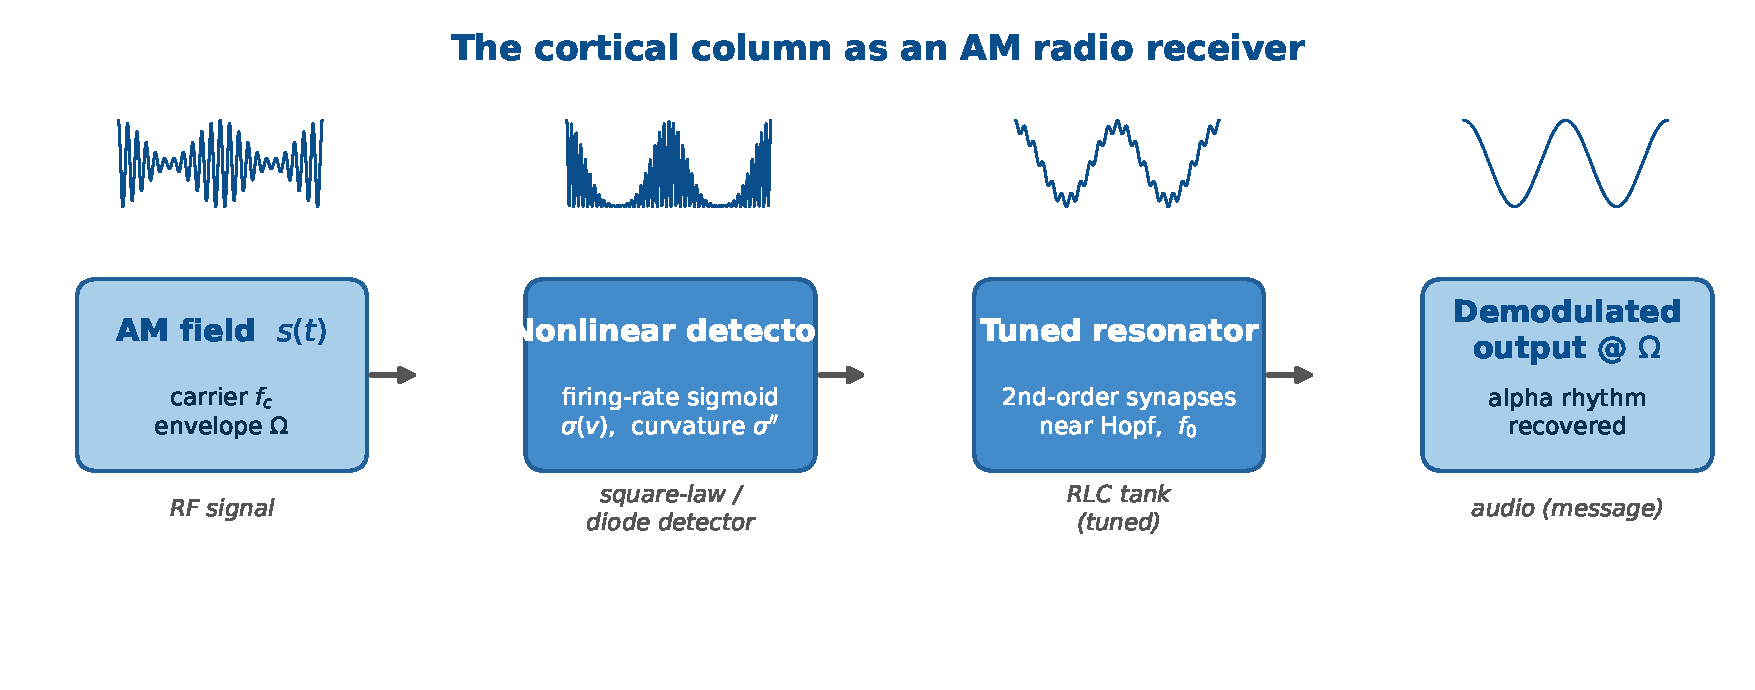
\includegraphics[width=\textwidth]{fig_concept.pdf}
%\vspace{-2cm}

\caption{\textbf{The cortical column as a tuned receiver.} Access converts the
applied field into the local polarization entering the detector. The nonlinear detector
generates the beat at angular frequency $\Omega$ from a carrier near $f_c$; a
recurrent network amplifies it near its natural frequency $f_0$. The diagram shows
the static-sigmoid realization. In a conventional AM receiver, the tuned circuit
selects the carrier before detection \cite{nahin2001}; here the resonator selects
the low-frequency output. \DIFdelbeginFL \DIFdelFL{The laminar extension also has a carrier-selective
stage (\S\ref{sec:lanmm-results}).}\DIFdelendFL }
\label{fig:concept}
\end{figure}

\section{Theory}

\subsection{\DIFdelbegin \DIFdel{Population transfer and }\DIFdelend \DIFaddbegin \DIFadd{A population rate curve supplies }\DIFaddend the \DIFdelbegin \DIFdel{slow-synapse limit}\DIFdelend \DIFaddbegin \DIFadd{nonlinearity}\DIFaddend }\label{sec:nmm}
A neural mass model describes a population through averaged variables
\cite{ruffini2025rosetta,jansen1995}. In the Jansen--Rit (JR) family, a linear synaptic
filter converts presynaptic firing rate $r(t)$ into postsynaptic potential $u_{\rm PSP}(t)$:
\[
\ddot u_{\rm PSP}+2a\dot u_{\rm PSP}+a^2u_{\rm PSP}=Aa\,r(t),
\]
with inverse synaptic time $a$ (s$^{-1}$) and PSP gain $A$ (mV); inhibitory synapses use
$b$ and $B$ in the same respective units. Summed postsynaptic potentials give the mean input $v$, which
a static transfer curve converts to firing rate \cite{wilsoncowan1972},
\begin{equation}
\Sig(v)=\frac{2e_0}{1+e^{\,\rho(v_0-v)}} .
\label{eq:sigmoid}
\end{equation}
Here $2e_0$ is the maximum rate, $v_0$ the inflection voltage, and $\rho$ the inverse
voltage scale (s$^{-1}$, mV, and mV$^{-1}$, respectively). Primes denote
derivatives with respect to voltage. Nonzero curvature makes this curve a mixer, while its slope sets
the local gain of the recurrent circuit.

\DIFdelbegin \DIFdel{For a synapse from population $Y$ to $X$, the resulting first-generation neural
mass model (NMM1) equations are
\cite{ruffini2025rosetta}
}\begin{displaymath}
\DIFdel{\hat L_{X\leftarrow Y}\big[u_{X\leftarrow Y}\big]=C_{X\leftarrow Y}\,r_Y,\qquad
v_X=\Lambda[E]+\!\!\sum_{Y:\,C_{X\leftarrow Y}\neq0}\!\!u_{X\leftarrow Y},\qquad
r_X=\Sig(v_X).
%DIFDELCMD < %%%
}\end{displaymath}%DIFAUXCMD
\DIFdel{The operator $\hat L$ is the inverse synaptic filter, $u_{X\leftarrow Y}$ its
postsynaptic potential, $C_{X\leftarrow Y}$ the connectivity, and $\Lambda[E]$
the direct polarization caused by the applied field $E$ (V/m). The rates $r_X,r_Y$
are in s$^{-1}$, the potentials $v_X,u_{X\leftarrow Y}$ in mV, and the
pathway weights $C_{X\leftarrow Y}$ dimensionless. This field contribution enters
alongside the synaptic potentials, without first passing through a synapse.
}%DIFDELCMD <

%DIFDELCMD < %%%
\DIFdel{The corresponding population nonlinearity can be derived for all-to-all coupled
QIF neurons with Lorentzian-distributed excitabilities. Their exact
Montbri\'o--Paz\'o--Roxin (MPR) mean field evolves the firing rate $r$ and mean voltage
$v$ \cite{montbrio2015}; adding dynamic synapses gives NMM2
\cite{ruffini2021nmm2,clusella2023}. With normalized time $\tilde t=t/\tau_m$ and rate $\tilde r=\tau_m r$, where $\tau_m$ is the membrane time,
}\begin{displaymath}
\DIFdel{\frac{\mathrm d\tilde r}{\mathrm d\tilde t}=\frac{\Delta}{\pi}+2\tilde r\,v,\qquad
\frac{\mathrm dv}{\mathrm d\tilde t}=v^2+\bar\eta-\pi^2\tilde r^2+I(\tilde t),
%DIFDELCMD < %%%
}\end{displaymath}%DIFAUXCMD
\DIFdel{where $\bar\eta$ is the mean excitability, $\Delta>0$ its half-width, and $I(\tilde t)$ the
normalized input, including recurrent drive when present. The reduced variables are dimensionless; $r$ without a tilde denotes physical
firing rate. For a constant total drive
$Q=\bar\eta+I$, setting both derivatives to zero gives $v=-\Delta/(2\pi\tilde r)$ and
}\begin{displaymath}
\DIFdel{\tilde r=F(Q)=\frac{1}{\pi}\sqrt{\frac{Q+\sqrt{Q^2+\Delta^2}}{2}} .
%DIFDELCMD < %%%
}\end{displaymath}%DIFAUXCMD
\DIFdel{Primes on $F$ denote derivatives with respect to the total drive $Q$.
Its curvature combines threshold recruitment and the concave rate increase of
active cells (App.~\ref{app:mpr-mixing}). This nonlinear curve exists
without recurrent coupling. It has an inflection at
$Q=\Delta/\sqrt3$ and an unbounded concave rise, unlike the saturating JR sigmoid.
}%DIFDELCMD <

%DIFDELCMD < %%%
\DIFdel{If the population relaxes to this equilibrium faster than synaptic inputs change,
NMM2 reduces to a static rate map with dynamic synapses
\cite{ruffini2021nmm2,clusella2023}. Restoring the membrane time $\tau_m$ and physical
firing rate, a second-order synapse with time constant $\tau_s$ obeys
}\begin{displaymath}
\DIFdel{r(t)\simeq \frac{F(Q(t))}{\tau_m},\qquad
\tau_s^2\ddot r_{\rm syn}+2\tau_s\dot r_{\rm syn}+r_{\rm syn}=r(t),
}\end{displaymath}%DIFAUXCMD
\DIFdel{where $r_{\rm syn}$ is the filtered rate entering the recurrent drive in $Q$, with the original
coupling normalization retained. This is the slow-synapse limit: shortening the
effective membrane time makes the transfer appear static while the network retains
its synaptic dynamics. The relevant separation is between the population relaxation
time $\tau_{\rm rel}$ and $\tau_s$. Applying the same static map directly to a
carrier of angular frequency $\omega_c$ requires the stronger condition
$\omega_c\tau_{\rm rel}\ll1$. A population can therefore be quasistatic for its
synaptic inputs yet dynamic for a kHz carrier.
}%DIFDELCMD <

%DIFDELCMD < %%%
\DIFdel{The transfer curve summarizes cellular nonlinearities within this regime. Its
curvature combines their leading contributions to mixing; its slope converts a
slow input into a rate change and enters recurrent gain. QIF supplies a derived
realization through its spike-generating quadratic and excitability distribution.
The generic weak-input mixing law does not require identifying each channel's
contribution, although the coefficient and its frequency dependence are
model-specific. Outside the static limit these contributions belong to a dynamic
input--output functional. Section~\ref{sec:dynamic} calculates this response for
QIF and recovers Eq.~\eqref{eq:Fmpr} in the adiabatic limit.
}%DIFDELCMD <

%DIFDELCMD < %%%
\DIFdel{The JR }\DIFdelend \DIFaddbegin \DIFadd{The JR }\DIFaddend column couples pyramidal, excitatory-interneuron, and inhibitory-interneuron
populations, with field input to the pyramidal sigmoid and local field potential
(LFP) proxy $v=y_1-y_2$, where $y_1$ and $y_2$ are the excitatory and inhibitory
postsynaptic potentials onto the pyramidal population. Its external input rate is
$p$ (s$^{-1}$), and $C$ is the dimensionless connectivity scale\DIFdelbegin \DIFdel{(App.
~\ref{app:models}). The laminar extension (LaNMM)
\cite{ruffini2025cfc,sanchezTodo2023} adds coupled alpha and gamma circuits: deep
pyramidal $P_1$, spiny-stellate (SS), and somatostatin (SST) populations, and a
superficial pyramidal $P_2$/PV circuit. These models retain dynamic synapses and
static rate curves; NMM2 and its spiking realization retain membrane dynamics as well.
The recurrent circuit can resonate without intrinsic cellular resonance
\cite{brunelhakim1999,brunelwang2003}; in the fast-membrane limit only its synaptic
modes remain, and resonances requiring finite membrane dynamics need not persist.
}\DIFdelend \DIFaddbegin \DIFadd{.
}\DIFaddend

Figure~\ref{fig:models} locates the field input, nonlinear detector, and
recurrent amplifier in the JR and \DIFdelbegin \DIFdel{NMM2 circuits.
}%DIFDELCMD <

%DIFDELCMD < %%%
%DIF <  Proposed caption and placement (Klaus, 2026-10-06; revised after Kaiti's review 2026-10-06).
%DIF <  Place after the model definitions in Theory (sec:nmm), before the first JR result.
\DIFdelend \DIFaddbegin \DIFadd{QIF circuits.
}\DIFaddend \begin{figure}[t!]
\centering
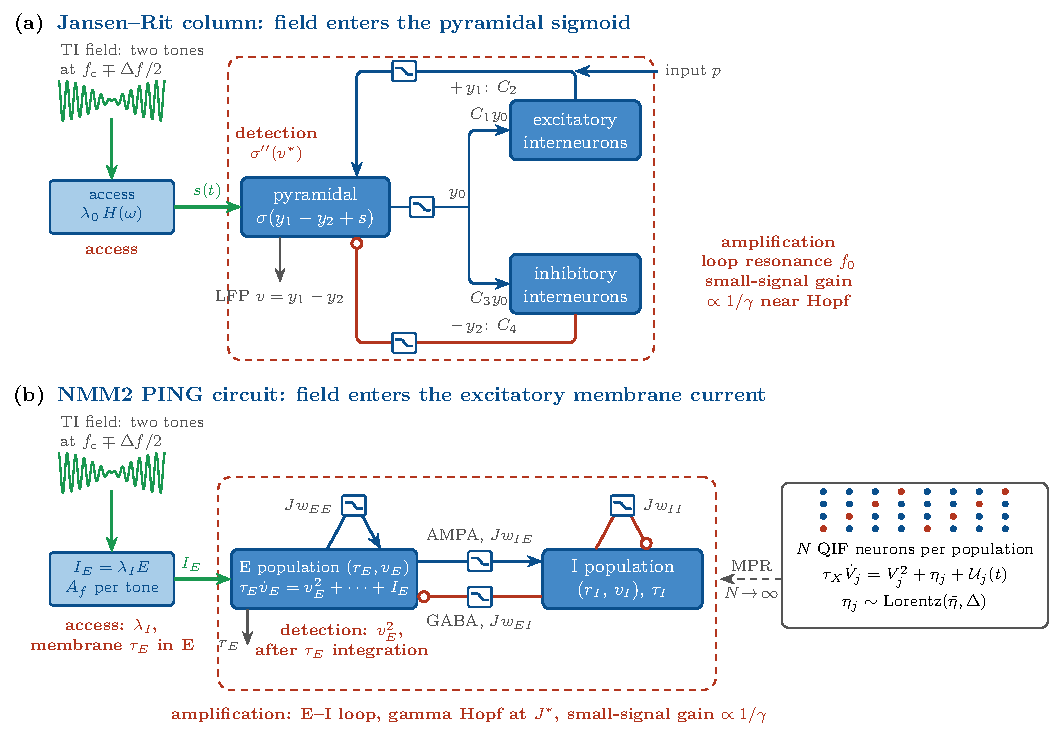
\includegraphics[width=\textwidth]{fig_models_ti.pdf}
\caption{\DIFdelbeginFL \DIFdelFL{\textbf{Where the TI field enters each model.} Both panels show the same three
stages, with each filter counted once. Access }\DIFdelendFL \DIFaddbeginFL \DIFaddFL{\textbf{Access, detection, and amplification in the two circuits.}
\emph{(a)} JR: access $\lambda_0H(\omega)$ }\DIFaddendFL converts the \DIFdelbeginFL \DIFdelFL{two-tone }\DIFdelendFL field \DIFdelbeginFL \DIFdelFL{into }\DIFdelendFL \DIFaddbeginFL \DIFaddFL{to polarization
$s$, and sigmoid curvature mixes }\DIFaddendFL the \DIFdelbeginFL \DIFdelFL{input
that reaches }\DIFdelendFL \DIFaddbeginFL \DIFaddFL{tones.
\emph{(b)} NMM2 PING: current $I_E=\lambda_I E$ enters }\DIFaddendFL the \DIFdelbeginFL \DIFdelFL{nonlinearity}\DIFdelendFL \DIFaddbeginFL \DIFaddFL{excitatory membrane}\DIFaddendFL ;
\DIFdelbeginFL \DIFdelFL{detection generates the beat; the recurrent circuit
amplifies it}\DIFdelendFL \DIFaddbeginFL \DIFaddFL{$v_E^2$ mixes its voltage excursions}\DIFaddendFL . \DIFdelbeginFL \DIFdelFL{Dashed outlines mark }\DIFdelendFL \DIFaddbeginFL \DIFaddFL{The inset shows }\DIFaddendFL the \DIFdelbeginFL \DIFdelFL{recurrent amplifier, }\DIFdelendFL \DIFaddbeginFL \DIFaddFL{QIF neurons }\DIFaddendFL whose
\DIFdelbeginFL \DIFdelFL{small-signal gain grows
as the inverse modal damping $1/\gamma$ near a Hopf bifurcation; $f_0$ is the mode's frequency}\DIFdelendFL \DIFaddbeginFL \DIFaddFL{infinite-population limit gives this exact mean field}\DIFaddendFL .
\DIFdelbeginFL \DIFdelFL{The low-pass symbol on each synaptic arrow marks a }\DIFdelendFL \DIFaddbeginFL \DIFaddFL{Low-pass symbols mark }\DIFaddendFL second-order \DIFdelbeginFL \DIFdelFL{low-pass filter
}\DIFdelendFL \DIFaddbeginFL \DIFaddFL{synapses }\DIFaddendFL (\DIFdelbeginFL \DIFdelFL{excitatory $h_e$ and inhibitory $h_i$ }\DIFdelendFL \DIFaddbeginFL \DIFaddFL{$h_e,h_i$ }\DIFaddendFL in \DIFdelbeginFL \DIFdelFL{\emph{a}}\DIFdelendFL \DIFaddbeginFL \DIFaddFL{a}\DIFaddendFL ; AMPA \DIFdelbeginFL \DIFdelFL{, $\tau_a$, }\DIFdelendFL and GABA
\DIFdelbeginFL \DIFdelFL{,
$\tau_g$, }\DIFdelendFL \DIFaddbeginFL \DIFaddFL{with times $\tau_a,\tau_g$ }\DIFaddendFL in \DIFdelbeginFL \DIFdelFL{\emph{b}}\DIFdelendFL \DIFaddbeginFL \DIFaddFL{b}\DIFaddendFL )\DIFdelbeginFL \DIFdelFL{acting after the nonlinearity}\DIFdelendFL . \DIFdelbeginFL \DIFdelFL{These filters attenuate
the carrier }\DIFdelendFL \DIFaddbeginFL \DIFaddFL{They suppress carriers }\DIFaddendFL more strongly than
the generated beat and transmit the steady shift\DIFdelbeginFL \DIFdelFL{into the recurrent loop}\DIFdelendFL .
\DIFdelbeginFL \DIFdelFL{\emph{(a)} Jansen--Rit column. Access multiplies the field by the static coupling
$\lambda_0$ and the access filter $H(\omega)$; the resulting polarization $s(t)$ enters
the pyramidal sigmoid}\DIFdelendFL \DIFaddbeginFL \DIFaddFL{Dashed frames enclose recurrent amplifiers}\DIFaddendFL , \DIFdelbeginFL \DIFdelFL{whose curvature $\sigma''(v^*)$ mixes the tones. The pyramidal
firing is filtered by the excitatory synaptic kernel $h_e$ (inverse time $a$, }\DIFdelendFL \DIFaddbeginFL \DIFaddFL{with small-signal }\DIFaddendFL gain
\DIFdelbeginFL \DIFdelFL{$A$)
}\DIFdelendFL \DIFaddbeginFL \DIFaddFL{proportional }\DIFaddendFL to \DIFdelbeginFL \DIFdelFL{give $y_0$. The interneurons receive $C_1y_0$ and $C_3y_0$, respectively, and
return }\DIFdelendFL \DIFaddbeginFL \DIFaddFL{$1/\gamma$ near }\DIFaddendFL the \DIFdelbeginFL \DIFdelFL{potentials $y_1$ (through $h_e$, connectivity $C_2$) and $y_2$ (through the
inhibitory kernel $h_i$, inverse time $b$, gain $B$, connectivity $C_4$). The external input is
$p$, and $v=y_1-y_2$ is the LFP proxy.
\emph{(b)} NMM2 PING circuit. The field enters the excitatory voltage equation as the
current $I_E=\lambda_I E$, of amplitude $A_f$ per tone; the excitatory membrane, with time
constant $\tau_E$, integrates it before the quadratic term $v_E^2$ mixes the tones.
Excitatory (AMPA, $\tau_a$) and inhibitory (GABA, $\tau_g$) synapses with global coupling
$J$ and pathway weights $w_{XY}$ (target $X$, source $Y$) close a gamma loop with a }\DIFdelendFL \DIFaddbeginFL \DIFaddFL{relevant }\DIFaddendFL Hopf\DIFdelbeginFL \DIFdelFL{bifurcation at $J^*$}\DIFdelendFL .
\DIFdelbeginFL \DIFdelFL{The population equations are the exact Montbri\'o--Paz\'o--Roxin
(MPR) mean field, in the limit $N\to\infty$, of the network of $N$ quadratic
integrate-and-fire neurons at right, with membrane time $\tau_X$ for $X\in\{E,I\}$
and $\mathcal U_j(t)$ the total
synaptic and field input to neuron $j$; the finite network is simulated directly in
\S\ref{sec:qif}. }\DIFdelendFL Blue\DIFdelbeginFL \DIFdelFL{arrows are excitatory, }\DIFdelendFL \DIFaddbeginFL \DIFaddFL{: excitation; }\DIFaddendFL red\DIFdelbeginFL \DIFdelFL{circle-ended connections inhibitory,
and }\DIFdelendFL \DIFaddbeginFL \DIFaddFL{: inhibition; }\DIFaddendFL green\DIFdelbeginFL \DIFdelFL{arrows carry the applied }\DIFdelendFL \DIFaddbeginFL \DIFaddFL{: }\DIFaddendFL field input.}
\label{fig:models}
\end{figure}


\subsection{From applied field to a squared-envelope beat component}\label{sec:coupling}
We \DIFdelbegin \DIFdel{use the quasistatic electromagnetic approximation for }\DIFdelend \DIFaddbegin \DIFadd{neglect electromagnetic propagation and induction in }\DIFaddend the applied field
$E(t)$ (V/m), \DIFdelbegin \DIFdel{neglecting propagation and induction. This does not make membranecharging
instantaneous}\DIFdelend \DIFaddbegin \DIFadd{while retaining the membrane's finite charging response}\DIFaddend . Let $s(t)$ be the
\DIFaddbegin \DIFadd{effective }\DIFaddend polarization (mV) \DIFdelbegin \DIFdel{after the cellular access response}\DIFdelend \DIFaddbegin \DIFadd{expressed in the sigmoid's input coordinate after cellular access}\DIFaddend ;
the static population model reads
\begin{equation}
r(t)=\Sig\!\big(v(t)+s(t)\big),\qquad
E(t)=E_1\cos\omega_1 t+E_2\cos\omega_2 t .
\label{eq:coupling}
\end{equation}
\DIFdelbegin \DIFdel{The field acts directly on soma}\DIFdelend \DIFaddbegin \DIFadd{Soma}\DIFaddend , dendrites, AIS, nodes, and terminals \DIFdelbegin \DIFdel{,
each with its own coupling and
frequency response }\DIFdelend \DIFaddbegin \DIFadd{have different couplings and
response times. We represent their contributions as parallel inputs}\DIFaddend .
\DIFdelbegin \DIFdel{In a reduced description, their contributions to the effective input are represented by parallel entry points.
}\DIFdelend For nearby carriers centered at $\omega_c=2\pi f_c$,
\begin{equation}
s(t)\simeq\sum_k \boldsymbol\lambda^k_f(\omega_c)\!\cdot\!\mathbf E(t),\qquad
\boldsymbol\lambda^k_f(\omega)=\boldsymbol\lambda^k_0\,\lvert H_k(\omega)\rvert,
\label{eq:doors}
\end{equation}
where $\boldsymbol\lambda^k_0$ is the static polarization vector of compartment $k$ (a length),
and $H_k$ its access filter
\cite{ruffini2025rosetta,galangadea2023}. Equation~\eqref{eq:doors} uses amplitude
gains and assumes aligned compartment phases; a general sum requires the complex
transfers, including their relative phases. The \DIFdelbegin \DIFdel{passive compartment equations in
App.~\ref{app:access} give both factors from the same voltage response.
The static gain and its frequency dependence belong to this
one response. A model driven by post-coupling polarization and a model driven by
current through its own membrane equation must therefore count that filtering once.
}\DIFdelend \DIFaddbegin \DIFadd{supplied polarization includes the access response.
}\DIFaddend

For a dominant entry point, define $\lambda_f(\omega)=\lambda_0|H(\omega)|$.
Then $\varepsilon_j=\lambda_f(\omega_j)E_j$ denotes the
polarization reaching the nonlinearity. \DIFdelbegin \DIFdel{The direct-coupling calculation takes
$\lambda_f\approx\lambda_0$ }\DIFdelend \DIFaddbegin \DIFadd{We first hold this local polarization fixed }\DIFaddend to isolate mixing and recurrent
amplification\DIFdelbegin \DIFdel{;
\S\ref{sec:khz} restores frequency-dependent access. Fast axonal access motivates
this limit; compartment anatomy enters the reduced model through
the coupling and response time, which must be calibrated for the preparation.
It also fixes the projection direction. A laminar direction for a pyramidal
axon initial segment, a local axon direction for a node, or an orientation
distribution for terminals defines a different access model. Isotropic averaging
is one possible distribution,
not an anatomical consequence of choosing terminals. Maximizing a geometric map over orientation gives an upper bound for that map
at each location; it does not identify the detector's orientation. The FEM
comparison in \S\ref{sec:fem-methods} therefore holds its chosen direction fixed
when changing the current ratio}\DIFdelend . \DIFaddbegin \DIFadd{At fixed applied field, its frequency dependence follows $H$.
Fast axonal compartments motivate the direct-coupling approximation
$\lambda_f\approx\lambda_0$. For coupling at the AIS, the additive input $s$
represents a change in spike-initiation drive: $\Sig(v+s)$ is the same
sigmoid with its effective threshold shifted from $v_0$ to $v_0-s$.
No backward transmission to the soma is required. Converting local AIS
polarization into $s$, and determining the compartment's response time,
require calibration in the preparation. Fast access alone does not establish
that the static sigmoid describes detection at the carrier frequency.
}\DIFaddend

Expanding $\Sig$ about a field-free operating voltage $v^*$ (mV) (a Volterra/Taylor expansion, as
in \cite{ruffini2025ham}) gives
$\Sig(v^*+s)\approx\Sig(v^*)+\Sig'(v^*)\,s+\half\Sig''(v^*)\,s^2+\dots$
The truncation requires $|s|\ll1/\rho\approx1.8$~mV and a nonzero second derivative
for quadratic mixing to be leading. Larger excursions require the full transfer curve.
The linear term preserves the two input frequencies. The quadratic cross term
generates their difference through the identity
$2\cos\omega_1t\cos\omega_2t=\cos\Omega t+\cos(\omega_1+\omega_2)t$.
Low-pass synaptic filtering suppresses the fast terms after mixing; membrane
filtering, when retained, already shapes the carrier polarization. We isolate
the slow source by a carrier average, before applying its frequency-dependent
network gain\DIFdelbegin \DIFdel{(\S\ref{sec:carrier})}\DIFdelend . The fast
$\cos^2\omega_jt$ terms average to $\half$ and the sum-frequency term to zero:
\begin{equation}
\big\langle\Sig(v^*+s)\big\rangle_c
=\Sig(v^*)+\tfrac14\Sig''(v^*)\,(\varepsilon_1^2+\varepsilon_2^2)
+\tfrac12\Sig''(v^*)\,\varepsilon_1\varepsilon_2\cos\Omega t+O(\varepsilon^4),
\label{eq:taylor}
\end{equation}
so a line appears at exactly the envelope frequency $\Omega$, with amplitude
\begin{equation}
Y_\Omega\simeq\half\,\Sig''(v^*)\,\varepsilon_1\varepsilon_2 ,
\label{eq:demod}
\end{equation}
Here $Y_\Omega$ is the signed rate amplitude before recurrent feedback, in s$^{-1}$;
$\varepsilon$ denotes a common small amplitude scale, and $\simeq$ means to leading
order in the polarizations, here and in what follows. The
same expansion leaves a constant (DC) term, $\tfrac14\Sig''(\varepsilon_1^2+\varepsilon_2^2)$,
which any read-out of the mean rate must include.

For a dynamic cellular response with synaptic input held fixed, define the
effective second-order coefficient $\chi^{(2)}$ by the complex beat amplitude
$Y_\Omega$,
\DIFdelbegin \[
\DIFdel{Y_\Omega\simeq\chi^{(2)}(\omega_2,-\omega_1)\,
\varepsilon_2\varepsilon_1,\qquad
r_\Omega(t)=\operatorname{Re}\!\left[Y_\Omega e^{i\Omega t}\right].
}\]%DIFAUXCMD
\DIFdelend \DIFaddbegin \begin{equation}
\DIFadd{Y_\Omega\simeq\chi^{(2)}(\omega_2,-\omega_1)\,
\varepsilon_2\varepsilon_1,\qquad
r_\Omega(t)=\operatorname{Re}\!\left[Y_\Omega e^{i\Omega t}\right].
\label{eq:chi2}
}\end{equation}\DIFaddend
Here \DIFdelbegin \DIFdel{$i^2=-1$, and }\DIFdelend $r_\Omega(t)$ is the generated rate component before recurrent feedback.
Thus $\chi^{(2)}$ has units s$^{-1}$mV$^{-2}$ when its input is polarization
and its output is physical rate. With this cosine-amplitude convention, the memoryless limit is
$\chi^{(2)}=\Sig''(v^*)/2$. Cellular processes \DIFdelbegin \DIFdel{can contribute to the same coefficient , with model-specific
frequency and state dependence: weak amplitude permits the expansionbut does not
remove memory, and }\DIFdelend \DIFaddbegin \DIFadd{contribute to this coefficient according to their state and
response times. Weak input permits a second-order expansion, but a response
that depends on input history retains frequency-dependent amplitude and phase.
If }\DIFaddend symmetry or cancellation \DIFdelbegin \DIFdel{can make the quadratic term vanish.
}%DIFDELCMD <

%DIFDELCMD < %%%
\DIFdel{Write $\mathcal A(t)$ for the nonnegative envelope of the local two-tone
polarization, in mV. The quadratic source follows $\mathcal A^2$, whose temporal
and spatial maps are derived in \S\ref{sec:envelope}.
}%DIFDELCMD <

%DIFDELCMD < %%%
\DIFdel{Dense perturbative sweeps use an amplitude-modulated (AM) surrogate that matches
}\DIFdelend \DIFaddbegin \DIFadd{makes this coefficient zero, higher orders determine
}\DIFaddend the leading beat\DIFdelbegin \DIFdel{source; its waveform and the two-tone controls are specified in
\S\ref{sec:waveforms}}\DIFdelend .

\DIFdelbegin \DIFdel{The same quadratic intermodulation generates endogenous AM sidebands from slow
and fast inputs \cite{ruffini2025ham}, or $\omega_0\pm\Omega$ sidebands when the
recovered beat mixes with an intrinsic rhythm $\omega_0$
(Fig.~\ref{fig:qif_timing}b).
}%DIFDELCMD <

%DIFDELCMD < %%%
\DIFdelend Equation~\eqref{eq:demod} carries \DIFdelbegin \DIFdel{three predictions, all verified below}\DIFdelend \DIFaddbegin \DIFadd{the static detector's predictions}\DIFaddend : the
generated beat is quadratic in the drive ($Y_\Omega\propto\varepsilon^2$,
square-law detection); it follows the sigmoid curvature
($Y_\Omega\propto\Sig''(v^*)$, hence zero at the inflection $v^*=v_0$); and, \emph{at
fixed post-coupling polarization} $\varepsilon$, it is independent of the carrier
$\omega_c$. This last prediction needs care: as a function of the \emph{applied} field the
response inherits the coupling $\varepsilon=\lambda_f E_0$, with applied amplitude $E_0$,
so \DIFaddbegin \DIFadd{attenuating access raises }\DIFaddend the field required for a given effect\DIFdelbegin \DIFdel{rises with $f_c$ (\S\ref{sec:khz})}\DIFdelend , consistent with the carrier
dependence of TI thresholds in \cite{opancar2025,peripheral2023}.
Carrier independence is thus a statement about the recovered beat component at fixed
polarization, not about the applied field.

\DIFdelbegin \subsection{\DIFdel{The exact mean field connects static and dynamic mixing}}%DIFAUXCMD
\addtocounter{subsection}{-1}%DIFAUXCMD
%DIFDELCMD < \label{sec:dynamic}
%DIFDELCMD < %%%
\DIFdel{The adiabatic condition in \S\ref{sec:nmm} determines whether the static curve describes
carrier mixing. Consider an uncoupled MPR population (Eq.~\eqref{eq:mpr}, membrane
time units), with constant drive $Q$ and a weak added current $I_{\rm ac}\cos(\tilde\omega\tilde t)$.
Here $\tilde\omega=\omega\tau_m$ is the normalized carrier angular frequency.
To second order in $I_{\rm ac}$, the carrier-averaged shift of $\tilde r$ is $I_{\rm ac}^2\kappa_{\rm DC}(Q,\tilde\omega)$, where
}\begin{displaymath}
\DIFdel{\kappa_{\rm DC}(Q,\tilde\omega)=\frac{\tilde r^*\,[\tilde\omega^2+3d^2-\nu^2]}{(d^2+\nu^2)\{[d^2+\nu^2-\tilde\omega^2]^2+4d^2\tilde\omega^2\}},
\qquad \tilde r^*=F(Q),\quad d=\frac{\Delta}{\pi \tilde r^*},\quad \nu=2\pi \tilde r^*.
%DIFDELCMD < %%%
}\end{displaymath}%DIFAUXCMD
\DIFdel{The physical rate shift is $I_{\rm ac}^2\kappa_{\rm DC}/\tau_m$.
The fixed-point eigenvalues in normalized time are $-d\pm i\nu$: $d$ is the relaxation rate and $\nu$
the ringing angular frequency, both in membrane-time units; their physical
values are $d/\tau_m$ and $\nu/\tau_m$. The expansion about the fixed point is given in
App.~\ref{app:mpr-mixing}. Its limits are
}\begin{displaymath}
\DIFdel{\kappa_{\rm DC}(Q,\tilde\omega)\xrightarrow[\ \tilde\omega\to0\ ]{}\tfrac14F''(Q),\qquad
\kappa_{\rm DC}(Q,\tilde\omega)\xrightarrow[\ \tilde\omega\gg d,\nu\ ]{}\frac{F'(Q)}{2\tilde\omega^2}.
}\end{displaymath}%DIFAUXCMD
\DIFdel{In the first limit the population tracks its static curve, whose curvature rectifies
the input. In the second, the voltage excursion is approximately $I_{\rm ac}/\tilde\omega$; its
square supplies a slow drive that the population reads through $F'$. Above the
inflection of $F$, these limits have opposite signs and the coefficient vanishes at
$\tilde\omega_z=\sqrt{\nu^2-3d^2}$ (Fig.~\ref{fig:crossover}a). The $300$~Hz and kHz carriers
are on the fast side for the parameters of the pyramidal--interneuron network gamma
(PING) circuit used below. That classification is
parameter-dependent: a shorter effective membrane time can bring the same physical
carrier into the adiabatic regime.
}%DIFDELCMD <

%DIFDELCMD < %%%
\DIFdel{Membrane access is already included in this calculation. The linear voltage response
is $H_v(\tilde\omega)=(i\tilde\omega+d)/[(i\tilde\omega+d)^2+\nu^2]$. Dividing by its squared magnitude
gives the mixing coefficient at fixed voltage excursion,
}\begin{displaymath}
\DIFdel{\kappa_V(Q,\tilde\omega)=\frac{\kappa_{\rm DC}(Q,\tilde\omega)}{|H_v(\tilde\omega)|^2}
=\frac{F'(Q)}{2}\;\frac{\tilde\omega^2+3d^2-\nu^2}{\tilde\omega^2+d^2}.
%DIFDELCMD < %%%
}\end{displaymath}%DIFAUXCMD
\DIFdel{This coefficient tends to $F'/2$ at high frequency. The $1/\tilde\omega^2$ suppression
at fixed current comes from $|H_v|^2$, the membrane filtering already represented
by Eq.~\eqref{eq:doors}; it is not an additional detector filter. A static curve
placed after the same membrane has the same leading carrier roll-off, although
its mixing coefficient and sign can differ. The steady-state curvature is
$F''=4\tilde r^*(3d^2-\nu^2)/(d^2+\nu^2)^3$, so the inflection occurs at $\nu^2=3d^2$.
}%DIFDELCMD <

%DIFDELCMD < %%%
\DIFdel{For nearby fast tones, the quadratic terms in Eq.~\eqref{eq:mpr} contribute at
different orders: $v^2$ at $\omega^{-2}$, $\tilde r v$ at $\omega^{-3}$, and $\tilde r^2$ at
$\omega^{-4}$. Table~\ref{tab:exponents} compares the carrier and beat routes to
the firing rate for a static curve and a dynamic population with the same membrane access.
}%DIFDELCMD <

%DIFDELCMD < \begin{table}[h]
%DIFDELCMD < \centering\small
%DIFDELCMD < \begin{tabular}{lcc}
%DIFDELCMD < \toprule
%DIFDELCMD < %%%
\DIFdelFL{stage }%DIFDELCMD < & %%%
\DIFdelFL{static curve, same membrane }%DIFDELCMD < & %%%
\DIFdelFL{dynamic population }%DIFDELCMD < \\
%DIFDELCMD < \midrule
%DIFDELCMD < %%%
\DIFdelFL{point-membrane current $\to$ voltage }%DIFDELCMD < & %%%
\DIFdelFL{$\omega^{-1}$ }%DIFDELCMD < & %%%
\DIFdelFL{$\omega^{-1}$ }%DIFDELCMD < \\
%DIFDELCMD < %%%
\DIFdelFL{voltage $\to$ rate, carrier }%DIFDELCMD < & %%%
\DIFdelFL{$1$ }%DIFDELCMD < & %%%
\DIFdelFL{$\omega^{-1}$ }%DIFDELCMD < \\
%DIFDELCMD < %%%
\DIFdelFL{current $\to$ rate, carrier }%DIFDELCMD < & %%%
\DIFdelFL{$\omega^{-1}$ }%DIFDELCMD < & %%%
\DIFdelFL{$\omega^{-2}$ }%DIFDELCMD < \\
%DIFDELCMD < %%%
\DIFdelFL{two tones $\to$ beat in the rate }%DIFDELCMD < & %%%
\DIFdelFL{$(\omega_1\omega_2)^{-1}$ }%DIFDELCMD < & %%%
\DIFdelFL{$(\omega_1\omega_2)^{-1}\times$ const. }%DIFDELCMD < \\
%DIFDELCMD < \bottomrule
%DIFDELCMD < \end{tabular}
%DIFDELCMD < %%%
%DIFDELCMD < \caption{%
{%DIFAUXCMD
\DIFdelFL{Fast-carrier scaling with matched point-membrane access, at fixed beat frequency
and a nonzero leading mixing coefficient. The dynamic population integrates the
carrier once more between voltage and rate; the beat is formed before that step.
Prefactors depend on the operating point and beat-frequency susceptibility.}}
%DIFAUXCMD
%DIFDELCMD < \label{tab:exponents}
%DIFDELCMD < \end{table}
%DIFDELCMD <

%DIFDELCMD < %%%
\DIFdel{The first row gives the shared membrane factor $1/\omega$. The second converts
voltage to rate: a static curve adds its slope, whereas the dynamic rate equation
integrates the carrier once more. Combining these stages gives the third-row
carrier responses, $\omega^{-1}$ and $\omega^{-2}$, respectively.
}%DIFDELCMD <

%DIFDELCMD < %%%
\DIFdel{The beat in the last row is formed before that additional rate integration:
static curvature and dynamic $v^2$ each mix the attenuated voltage, retaining
$(\omega_1\omega_2)^{-1}$. Equal exponents do not imply equal amplitudes; mixing
and the susceptibility at fixed $\Omega$ determine the prefactors. For the
uncoupled carrier-averaged response, $\kappa_V$ in Eq.~\eqref{eq:kfixed} tends to
$F'/2$, but is not the full finite-$\Omega$ network prefactor. Thus the dynamic
rate attenuates the carrier twice while forming the beat between those stages.
}%DIFDELCMD <

%DIFDELCMD < %%%
\subsection{\DIFdel{Detector laws and harmonic signatures}}%DIFAUXCMD
\addtocounter{subsection}{-1}%DIFAUXCMD
%DIFDELCMD < \label{sec:transduction}
%DIFDELCMD < %%%
\DIFdel{A neural response proportional to the squared envelope is not equivalent to one
proportional to the envelope. A detector implements some transduction $T(\mathcal A)$ of the local
envelope $\mathcal A(t)$, and the two laws predict different amplitude scaling, harmonic content and
spatial weighting.
}%DIFDELCMD <

%DIFDELCMD < %%%
\DIFdel{For a narrowband field $s(t)=\mathcal A(t)\cos\omega_c t$ passing through a memoryless nonlinearity
$g$, the low-frequency (baseband) output $Y_{\rm LF}$ is the average of $g$ over one
carrier cycle, with carrier phase $\theta$:
}\[
\DIFdel{Y_{\rm LF}(\mathcal A)=(2\pi)^{-1}\!\int_0^{2\pi}\!g(v^*+\mathcal A\cos\theta)\,\mathrm{d}\theta.
}\]%DIFAUXCMD
\DIFdel{Odd powers of $\mathcal A$ average away, leaving only even ones:
}\begin{displaymath}
\DIFdel{Y_{\rm LF}(\mathcal A)=g(v^*)+\tfrac14 g''(v^*)\mathcal A^2+\tfrac1{64}g^{(4)}(v^*)\mathcal A^4+\cdots
%DIFDELCMD < %%%
}\end{displaymath}%DIFAUXCMD
\DIFdel{A smooth memoryless response with $g''(v^*)\neq0$ therefore transduces $\mathcal A^2$ at
leading weak-input order, whatever its detailed shape. For the JR column, $g=\Sig$, giving the
mechanism of \S\ref{sec:coupling}. Recovering $\mathcal A$ itself requires a qualitatively
different detector: strong rectification. A full-wave rectifier has low-pass-filtered (LPF) output
$\mathrm{LPF}[\,|\mathcal A\cos\omega_c t|\,]=(2/\pi)\mathcal A$ and a half-wave rectifier
$(1/\pi)\mathcal A$, both linear in the envelope, as does a diode-and-capacitor peak detector.
A hard threshold is not one of them: a step detector with offset $\delta>0$ transduces
$\pi^{-1}\arccos(\delta/\mathcal A)$ for $\mathcal A>\delta$ and nothing below it, which is neither linear
nor quadratic in $\mathcal A$ (App.~\ref{app:bound}). Asymmetric channel rectification, threshold
crossing and release events are candidate biological realizations of rectifiers of one
kind or another.
}%DIFDELCMD <

%DIFDELCMD < %%%
\DIFdel{Envelope following and square-law detection are distinguishable at a single site. At a matched target,
$\mathcal A(t)=2\varepsilon|\cos(\Omega t/2)|$, whose Fourier series
$|\cos\theta|=\tfrac2\pi+\tfrac4\pi\sum_{n\ge1}\tfrac{(-1)^{n+1}}{4n^2-1}\cos(2n\theta)$ gives a
harmonic ladder whose nonnegative Fourier amplitudes $A_{n\Omega}$ obey $A_{2\Omega}/A_\Omega=1/5$, $A_{3\Omega}/A_\Omega=3/35$ and
$A_{4\Omega}/A_\Omega=1/21$. The square-law output $\half \mathcal A^2=\varepsilon^2(1+\cos\Omega
t)$ contains only DC and $\Omega$. For the mixed family $T(\mathcal A)=c_1\mathcal A+c_2\mathcal A^2$, with
$c_1\ne0$ and a nonzero fundamental, the
pre-network ratio is
}\begin{displaymath}
\DIFdel{\mathcal H_{\rm det}\equiv\left|\frac{Y_{2\Omega}}{Y_\Omega}\right|
=\frac{1/5}{\left|1+\tfrac{3\pi}{4}\,c_2\varepsilon/c_1\right|},
%DIFDELCMD < %%%
}\end{displaymath}%DIFAUXCMD
\DIFdel{so measuring $\mathcal H_{\rm det}$ constrains $c_2\varepsilon/c_1$ within this family.}\footnote{\DIFdel{The inverse has two branches unless the sign of the fundamental
relative to the linear term is known; for $c_2/c_1\ge0$ it is unique.}}
%DIFAUXCMD
\addtocounter{footnote}{-1}%DIFAUXCMD
%DIFDELCMD <

%DIFDELCMD < %%%
\DIFdel{A smooth detector generates a second harmonic beyond quadratic order,
$Y_{2\Omega}/Y_\Omega\sim(c_4/c_2)\varepsilon^2$, where
$c_2=g''(v^*)/4$ and $c_4=g^{(4)}(v^*)/64$ are the coefficients in
Eq.~\eqref{eq:cycavg}. The square-law signature is a
\emph{vanishing} ratio in the weak-field limit, not an exact zero. The recurrent
network also multiplies each harmonic by its frequency-dependent gain $G$,
$\mathcal H_{\rm meas}=\mathcal H_{\rm det}\,|G(2\Omega)/G(\Omega)|$.
Near resonance, harmonic suppression can make an envelope follower appear square-law.
}%DIFDELCMD <

%DIFDELCMD < %%%
\DIFdel{An amplitude sweep tests the scaling rather than one ratio. An
envelope-following detector gives $Y_\Omega\propto\varepsilon$ with the harmonic ratio
pinned at $1/5$; a weak square-law detector gives $Y_\Omega\propto\varepsilon^2$ with a
ratio growing as $\varepsilon^2$. A threshold detector is a third class: its
response vanishes for $2\varepsilon\le\delta$, and its harmonic ratio varies
with amplitude after onset. A single harmonic ratio cannot distinguish all
three; amplitude dependence is the primary test.
}%DIFDELCMD <

%DIFDELCMD < %%%
\DIFdelend \subsection{Envelope oscillations and spatial weighting}\label{sec:envelope}
The same two-tone field gives different spatial dose maps under envelope following
and quadratic detection. The distinction is the detector's response to the
oscillating envelope, not a change in the applied field.
Write $\mathbf x$ for position and $\varepsilon_j(\mathbf x)$ for the signed local
polarization of tone $j$, projected along a fixed direction. These amplitudes vary
in space and are held fixed only during the temporal averages at one location.
The nonnegative envelope is
\[
\mathcal A(\mathbf x,t)=\sqrt{\varepsilon_1(\mathbf x)^2+\varepsilon_2(\mathbf x)^2
+2\varepsilon_1(\mathbf x)\varepsilon_2(\mathbf x)\cos\Omega t}.
\]
Carrier averaging of the squared signal gives
\begin{equation}
\mathrm{LPF}[s^2(t)]=\tfrac12\mathcal A^2(t)
=\frac{\varepsilon_1^2+\varepsilon_2^2}{2}+\varepsilon_1\varepsilon_2\cos\Omega t,
\label{eq:sqenv}
\end{equation}
with spatial arguments suppressed at a fixed location. Thus square-law detection recovers $\mathcal A^2$,
which is sinusoidal at $\Omega$, whereas the envelope itself is not: at a matched
site, $\mathcal A(t)=2\varepsilon|\cos(\Omega t/2)|$, a rectified cosine.
The conventional TI map describes its excursion,
$\mathcal{M}[y]\equiv\max_t y-\min_t y$, along the chosen direction \cite{grossman2017}.
Table~\ref{tab:transduction-maps} compares this envelope with the squared-envelope
signal; the overbar denotes a beat-period mean. The geometric maps precede detector gains: an ideal envelope follower \DIFdelbegin \DIFdel{multiplies $\mathcal A$ by its }\DIFdelend \DIFaddbegin \DIFadd{has
response $c_1\mathcal A$ for a }\DIFaddend specified gain $c_1$\DIFdelbegin \DIFdel{, whereas the weak quadratic response change is }\DIFdelend \DIFaddbegin \DIFadd{. A smooth transfer $g$
with nonzero curvature gives the weak response }\DIFaddend $g''(v^*)\mathcal A^2/4$\DIFdelbegin \DIFdel{(Eq.~\eqref{eq:cycavg})}\DIFdelend ;
for the JR column, $g=\Sig$.
The last row carries these gains into the signed steady source. In particular,
the nonnegative mean-square polarization $\mathcal I$ alone does not specify
excitation or suppression.
Envelope following is an additional response assumption; the conventional
envelope-excursion map alone does not specify a neuron's mean output.

\begin{table}[ht]
\centering\small
\renewcommand{\arraystretch}{1.4}
\begin{tabular}{@{}>{\raggedright\arraybackslash}p{0.22\textwidth}
 >{\raggedright\arraybackslash}p{0.34\textwidth}
 >{\raggedright\arraybackslash}p{0.36\textwidth}@{}}
\toprule
 & Envelope following & Quadratic detection \\
\midrule
Slow signal & $\mathcal A(\mathbf x,t)$ & $\tfrac12\mathcal A(\mathbf x,t)^2$ \\
Mean before gain & $\overline{\mathcal A}(\mathbf x)$
 & $\mathcal I(\mathbf x)=\dfrac{\varepsilon_1^2+\varepsilon_2^2}{2}$ \\
Modulation excursion & $2\min(|\varepsilon_1|,|\varepsilon_2|)$
 & $2|\varepsilon_1\varepsilon_2|$ \\
Units before detector gain & mV & mV$^2$ \\
Signed steady source (output units) & $c_1\overline{\mathcal A}$
 & $Y_{\rm DC}=\tfrac12g''(v^*)\mathcal I$ \\
\bottomrule
\end{tabular}
\caption{Envelope and quadratic maps at the same position $\mathbf x$.
The first four rows give geometric quantities before detector gain; the last
gives the steady source after gain, before recurrent feedback. Its sign depends
on the detector. Averaging the slow signal over a beat period gives its mean.
Excursion means maximum minus minimum, not Fourier amplitude.}
\label{tab:transduction-maps}
\end{table}

The excursion maps in Table~\ref{tab:transduction-maps} are related pointwise by
\begin{equation}
\mathcal{M}\big[\tfrac12\mathcal A^2\big]=\max(|\varepsilon_1|,|\varepsilon_2|)\;\mathcal{M}[\mathcal A].
\label{eq:reweight}
\end{equation}
The square-law map is the conventional envelope-excursion map multiplied, at each point,
by the dominant local polarization magnitude. It need not preserve the spatial contrast
of the conventional TI map. Both maps can nevertheless have a central modulation
maximum, as the illustrative line profile in Fig.~\ref{fig:spatial_maps}a shows;
the quadratic profile is broader in that example. Where the dominant carrier is larger superficially than at depth,
this reweighting degrades deep-to-superficial contrast. As an illustrative example, at
$(\varepsilon_1,\varepsilon_2)=(10,1)$ superficially against $(0.5,0.5)$ at a matched
deep target, $\mathcal{M}[\mathcal A]$ favors the superficial point by $2\times$ and
$\mathcal{M}[\half \mathcal A^2]$ by $40\times$. Focality must therefore be computed from the product map, whose spatial ranking
can differ from the envelope map's. Its contrast depends on the actual vector
field distribution: a sufficiently weak second carrier can suppress the
superficial product. The \DIFdelbegin \DIFdel{finite-element comparison in \S\ref{sec:fem-results}
quantifies this reweighting on one realistic TI montage: at balanced currents,
the target-to-reference contrast is 1.22 for the envelope and 1.08 for the square root of the quadratic map. This is a milder change than the illustrative
two-site contrast above; the line profile is not a head-model calculation}\DIFdelend \DIFaddbegin \DIFadd{line profile and two-site example illustrate the algebra; a realistic
contrast requires fields computed on a head model}\DIFaddend .

With one fixed electrode pair per carrier and fixed neural state, changing the
current ratio rescales the leading quadratic beat map without moving its maxima.
For fixed frequencies,
linear access, and fixed projection directions, write
$\varepsilon_j(\mathbf x)=I_j^{\rm pair}\mathcal P_j(\mathbf x)$, where
$I_j^{\rm pair}>0$ is the peak pair current (mA) and $\mathcal P_j$ is the signed
local polarization per unit current (mV/mA). Then
\[
\mathcal M[\tfrac12\mathcal A^2]
=2I_1^{\rm pair}I_2^{\rm pair}|\mathcal P_1\mathcal P_2|.
\]
The normalized map and its ratios between fixed target and reference regions are unchanged, as
Cassar\`a et al.\ noted for second-order mixing \cite{cassara2025part2}.
Fixed detector coefficients and linear network propagation preserve this common
current factor, including for dynamic mixing and spatially heterogeneous gains.
Steering within this regime requires changing at least one carrier's field shape,
for example by redistributing current among several electrodes at that frequency.
The mean-square polarization map, however, weights $\mathcal P_1^2$ and
$\mathcal P_2^2$ separately by the squared currents. It changes with the ratio;
after signed detection, the resulting steady source can indirectly reshape the
beat response by shifting local operating points. Threshold effects can also
break the quadratic prediction; the conventional $2\min$ steering law applies
when the detector follows the envelope. An interior beat maximum remains
compatible with the fixed-state product law.

The \DIFdelbegin \DIFdel{network supplies dynamical selectivity in addition to this spatial weighting. Writing
$R_\Omega(\mathbf{x})$ for the complex demodulated response at the envelope frequency $\Omega$
produced at location $\mathbf{x}$, and $G_{\mathbf{x}}(\Omega)$ for the local network susceptibility there,
}\begin{displaymath}
\DIFdel{R_\Omega(\mathbf{x})\;\propto\;\Sig''(v^*_{\mathbf{x}})\;G_{\mathbf{x}}(\Omega)\;
\varepsilon_1(\mathbf{x})\,\varepsilon_2(\mathbf{x}),
%DIFDELCMD < %%%
}\end{displaymath}%DIFAUXCMD
\DIFdel{a product of three factors.Field overlap sets where a difference-frequency drive is
generated at all; the
operating point and the network susceptibility set which of the
driven populations amplifies it. Resonance does not override }\DIFdelend \DIFaddbegin \DIFadd{local response weights the carrier product by the detector curvature and
network susceptibility (Eq.~\eqref{eq:receiver}). Field overlap supplies the
source; local physiology sets its sign and amplification. Resonance can compensate
for }\DIFaddend an unfavorable field product \DIFdelbegin \DIFdel{, but it can compensate for one}\DIFdelend \DIFaddbegin \DIFadd{but requires a nonzero source}\DIFaddend .

\DIFdelbegin \DIFdel{Equation~\eqref{eq:spatial} is written for }\DIFdelend \DIFaddbegin \DIFadd{The spatial maps use }\DIFaddend scalar projected fields. In general the
coupling is vectorial and compartment-specific,
$\varepsilon_i(\mathbf{x})=\boldsymbol{\lambda}\!\cdot\!\mathbf{E}_i(\mathbf{x})$, so the
mixing product $(\boldsymbol{\lambda}\!\cdot\!\mathbf{E}_1)
(\boldsymbol{\lambda}\!\cdot\!\mathbf{E}_2)$ is signed: its magnitude follows the product
of the projected amplitudes, while its phase inverts with either the sign of $\Sig''$ or
the relative sign of the two projections. The \DIFdelbegin \DIFdel{derivations below take the collinear, scalar case. }\DIFdelend \DIFaddbegin \DIFadd{scalar formulas use these fixed projections.
}\DIFaddend

\DIFaddbegin \subsection{\DIFadd{Detector laws and harmonic signatures}}\label{sec:transduction}
\DIFadd{A neural response proportional to the squared envelope is not equivalent to one
proportional to the envelope. A detector implements some transduction $T(\mathcal A)$ of the local
envelope $\mathcal A(t)$, and the two laws predict different amplitude scaling, harmonic content and
spatial weighting.
}

\DIFadd{For a narrowband field $s(t)=\mathcal A(t)\cos\omega_c t$ passing through a memoryless nonlinearity
$g$, the low-frequency (baseband) output $Y_{\rm LF}$ is the average of $g$ over one
carrier cycle, with carrier phase $\theta$:
}\[
\DIFadd{Y_{\rm LF}(\mathcal A)=(2\pi)^{-1}\!\int_0^{2\pi}\!g(v^*+\mathcal A\cos\theta)\,\mathrm{d}\theta.
}\]
\DIFadd{Odd powers of $\mathcal A$ average away, leaving only even ones:
}\begin{equation}
\DIFadd{Y_{\rm LF}(\mathcal A)=g(v^*)+\tfrac14 g''(v^*)\mathcal A^2+\tfrac1{64}g^{(4)}(v^*)\mathcal A^4+\cdots
\label{eq:cycavg}
}\end{equation}
\DIFadd{A smooth memoryless response with $g''(v^*)\neq0$ therefore transduces $\mathcal A^2$ at
leading weak-input order, whatever its detailed shape. For the JR column, $g=\Sig$, giving the
mechanism of \S\ref{sec:coupling}. Recovering $\mathcal A$ itself requires a qualitatively
different detector: strong rectification. A full-wave rectifier has low-pass-filtered (LPF) output
$\mathrm{LPF}[\,|\mathcal A\cos\omega_c t|\,]=(2/\pi)\mathcal A$ and a half-wave rectifier
$(1/\pi)\mathcal A$, both linear in the envelope, as does a diode-and-capacitor peak detector.
A hard threshold is not one of them: a step detector with offset $\delta>0$ transduces
$\pi^{-1}\arccos(\delta/\mathcal A)$ for $\mathcal A>\delta$ and nothing below it, which is neither linear
nor quadratic in $\mathcal A$. Asymmetric channel rectification, threshold
crossing and release events are candidate biological realizations of rectifiers of one
kind or another.
}

\DIFadd{At matched carrier amplitudes, the rectified-cosine envelope has a
second-to-first harmonic ratio of $1/5$, whereas the quadratic output contains
only the steady term and the fundamental. The full harmonic series and an
inversion for mixed linear/quadratic detectors are given in the supplement
(\S\ref{supp:harmonics}).
}\ifjne\else
\subsection{\DIFadd{Harmonic ladder and mixed detectors}}\label{supp:harmonics}
\DIFadd{Envelope following and square-law detection are distinguishable at a single site. At a matched target,
$\mathcal A(t)=2\varepsilon|\cos(\Omega t/2)|$, whose Fourier series
$|\cos\theta|=\tfrac2\pi+\tfrac4\pi\sum_{n\ge1}\tfrac{(-1)^{n+1}}{4n^2-1}\cos(2n\theta)$ gives a
harmonic ladder whose nonnegative Fourier amplitudes $A_{n\Omega}$ obey $A_{2\Omega}/A_\Omega=1/5$, $A_{3\Omega}/A_\Omega=3/35$ and
$A_{4\Omega}/A_\Omega=1/21$. The square-law output $\half \mathcal A^2=\varepsilon^2(1+\cos\Omega
t)$ contains only DC and $\Omega$. For the mixed family $T(\mathcal A)=c_1\mathcal A+c_2\mathcal A^2$, with
$c_1\ne0$ and a nonzero fundamental, the
pre-network ratio is
}\begin{equation}
\DIFadd{\mathcal H_{\rm det}\equiv\left|\frac{Y_{2\Omega}}{Y_\Omega}\right|
=\frac{1/5}{\left|1+\tfrac{3\pi}{4}\,c_2\varepsilon/c_1\right|},
\label{eq:rdet}
}\end{equation}
\DIFadd{so measuring $\mathcal H_{\rm det}$ constrains $c_2\varepsilon/c_1$ within this family.}\footnote{\DIFadd{The inverse has two branches unless the sign of the fundamental
relative to the linear term is known; for $c_2/c_1\ge0$ it is unique.}}

\fi

\DIFadd{A smooth detector generates a second harmonic beyond quadratic order,
$Y_{2\Omega}/Y_\Omega\sim(c_4/c_2)\varepsilon^2$, where
$c_2=g''(v^*)/4$ and $c_4=g^{(4)}(v^*)/64$ are the coefficients in
Eq.~\eqref{eq:cycavg}. The square-law signature is a harmonic ratio tending to zero with input strength. The recurrent
network also multiplies each harmonic by its frequency-dependent gain $G$,
$\mathcal H_{\rm meas}=\mathcal H_{\rm det}\,|G(2\Omega)/G(\Omega)|$.
Near resonance, harmonic suppression can make an envelope follower appear square-law.
}

\DIFadd{An amplitude sweep tests the scaling rather than one ratio. An
envelope-following detector gives $Y_\Omega\propto\varepsilon$ with the harmonic ratio
pinned at $1/5$; a weak square-law detector gives $Y_\Omega\propto\varepsilon^2$ with a
ratio growing as $\varepsilon^2$. A threshold detector is a third class: its
response vanishes for $2\varepsilon\le\delta$, and its harmonic ratio varies
with amplitude after onset. A single harmonic ratio cannot distinguish all
three; amplitude dependence is the primary test.
}

\DIFaddend \subsection{The steady source has a state-dependent sign}\label{sec:dc}
Mean-square polarization is a nonnegative geometric map. Detection converts it
into a signed\DIFaddbegin \DIFadd{, DC-like }\DIFaddend steady source, and the circuit converts that source into a mean
response. \DIFaddbegin \DIFadd{\emph{DC-like} refers to the detected source, not to a DC component in the applied
field. }\DIFaddend Under uniform conductivity, access, \DIFaddbegin \DIFadd{orientation, }\DIFaddend and detection, the source's
largest magnitude lies on \DIFdelbegin \DIFdel{compartment }\DIFdelend \DIFaddbegin \DIFadd{tissue-compartment }\DIFaddend boundaries; the envelope-following mean
obeys the same restriction\DIFdelbegin \DIFdel{, as shown below}\DIFdelend .
The envelope mean is
\[
\overline{\mathcal A}(\mathbf x)=\frac{1}{2\pi}\int_0^{2\pi}
\sqrt{\varepsilon_1(\mathbf x)^2+\varepsilon_2(\mathbf x)^2
+2\varepsilon_1(\mathbf x)\varepsilon_2(\mathbf x)\cos\vartheta}\,\mathrm d\vartheta,
\]
where $\vartheta$ is beat phase. At a matched site with
$\varepsilon_1=\varepsilon_2=\varepsilon>0$, the envelope and quadratic means are
$4\varepsilon/\pi$ and $\varepsilon^2$, respectively. \DIFdelbegin \DIFdel{The applied field has no DC
component: these means describe the ideal }\DIFdelend \DIFaddbegin \DIFadd{These means become }\DIFaddend detector outputs after multiplication by their gains\DIFdelbegin \DIFdel{, and }\DIFdelend \DIFaddbegin \DIFadd{; }\DIFaddend the
quadratic response change takes the sign of $g''$.
Even one carrier gives either ideal detector a mean output, but no beat modulation;
adaptation can alter the physiological mean response.

For the JR quadratic detector, the local rate source in Eq.~\eqref{eq:taylor} is
\[
Y_{\rm DC}(\mathbf x,\mathbf n)
=\frac{\Sig''(v^*_{\mathbf x})}{2}\,\mathcal I(\mathbf x,\mathbf n),
\qquad
\mathcal I(\mathbf x,\mathbf n)
=\frac{\varepsilon_1(\mathbf x,\mathbf n)^2+
\varepsilon_2(\mathbf x,\mathbf n)^2}{2}\ge0.
\]
Here $v^*_{\mathbf x}$ is the baseline voltage at position $\mathbf x$ and
$\mathbf n$ is the unit cell orientation used for both signed polarizations.
The source $Y_{\rm DC}$ is positive on the convex part of the rate curve,
negative on its concave part, and zero to this order at the inflection.
Reversing either carrier's polarity or $\mathbf n$ leaves the squares unchanged;
other directions change their magnitudes, while the sign remains set by the fixed curvature.
Figure~\ref{fig:spatial_maps}c shows both signs using one positive normalization.
At the pinned JR operating point $v^*=8.30$~mV, $\Sig''<0$, so the static
source lowers the local rate.
The observed mean-rate change also depends on which populations receive the
source and on recurrent feedback\DIFdelbegin \DIFdel{; the JR examples in \S\ref{sec:timing} have
a negative mean-rate shift}\DIFdelend .

\DIFdelbegin \DIFdel{The coefficient depends on the detector regime. For an uncoupled QIF population
at fast carriers, $v^2$ generates a positive effective input shift, and the
readout through $F'>0$ gives a positive rate shift. In the slow-carrier
(adiabatic) limit, $\kappa_{\rm DC}\to F''/4$, so the rate shift is negative
above the inflection of $F$ (Eq.~\eqref{eq:crossover_limits}). The positive
E-drive shift in \S\ref{sec:qif} is therefore a fast-carrier result for that
model; the mean-rate response after recurrent feedback need not retain its sign.
}%DIFDELCMD <

%DIFDELCMD < %%%
\DIFdelend Carrier averaging retains the cross term as the beat;
averaging over many beat cycles removes it, leaving a sum of intensities without
cross-frequency cancellation. At the detector output, where $Y_{\rm DC}\ne0$,
$|Y_\Omega/Y_{\rm DC}|=2|\varepsilon_1\varepsilon_2|/
(\varepsilon_1^2+\varepsilon_2^2)\le1$, with equality at matched tone magnitudes.
A common access factor cancels from this local ratio. In the polarization
mean-square map $\mathcal I=(\varepsilon_1^2+\varepsilon_2^2)/2$, the example
above gives $50.5$ superficially and $0.25$ at depth, a $202$-fold contrast;
the beat/DC ratios are $0.20$ and $1$, respectively.

The geometric restriction follows in a homogeneous, isotropic, source-free conductor. Writing $\phi_j$ for the potential of tone $j$, the
potentials $\phi_j$, each component of $\mathbf E_j=-\nabla\phi_j$, and the
signed polarizations $\varepsilon_j=\boldsymbol\lambda\cdot\mathbf E_j$ for
spatially fixed coupling $\boldsymbol\lambda$ are harmonic. Thus
$\nabla^2\mathcal I=\sum_j|\nabla\varepsilon_j|^2\ge0$: the intensity map is
subharmonic and has no strict interior maximum. A montage can shape each
carrier field, but the maximum of this map lies on the region's boundary;
conductivity interfaces are such boundaries.
For a spatially constant nonzero detector coefficient, this bounds the magnitude
of $Y_{\rm DC}$. A negative coefficient makes the source most negative at the
boundary. Spatially varying coefficients require a separately weighted map.

The envelope mean \DIFaddbegin \DIFadd{is also subharmonic under these assumptions: at each beat
phase it is the norm of a vector of harmonic functions, and phase averaging
preserves subharmonicity (supplement, \S\ref{supp:envelope-proof}).
}\ifjne\else
\subsection{\DIFadd{Envelope-mean subharmonicity}}\label{supp:envelope-proof}
\DIFadd{The envelope mean }\DIFaddend has the same restriction. At each beat phase $\vartheta$,
$\mathcal A$ is the Euclidean norm of
$(\varepsilon_1+\varepsilon_2\cos\vartheta,\,\varepsilon_2\sin\vartheta)$,
a vector of harmonic functions. A norm is convex, so this envelope is subharmonic;
averaging over $\vartheta$ preserves that property. Thus both idealized mean maps
lack a strict interior maximum under these conditions (Fig.~\ref{fig:spatial_maps}b).
\DIFaddbegin

\fi
\DIFaddend This does not prohibit a beat maximum: the product instead obeys
$\nabla^2(\varepsilon_1\varepsilon_2)=2\nabla\varepsilon_1\cdot\nabla\varepsilon_2$,
whose sign is unrestricted. Within the homogeneous model, interior selectivity
must therefore come from the oscillatory response rather than from either mean map.

Spatially varying access, orientation, or curvature can change the signed-source
map and the resulting physiological mean-response map. The intensity result does
not extend to these weighted responses. For \DIFaddbegin \DIFadd{isotropic orientations with orientation-independent access and curvature,
orthogonal fields cancel the averaged beat but retain the steady intensity
(supplement, \S\ref{supp:orientation}).
}\ifjne\else
\subsection{\DIFadd{Isotropic orientation averages}}\label{supp:orientation}
\DIFadd{For }\DIFaddend isotropically distributed unit orientations
$\mathbf n$ with orientation-independent access and curvature,
$\langle(\mathbf n\cdot\mathbf E_j)^2\rangle=|\mathbf E_j|^2/3$
and $\langle(\mathbf n\cdot\mathbf E_1)(\mathbf n\cdot\mathbf E_2)\rangle
=\mathbf E_1\cdot\mathbf E_2/3$: orthogonal fields cancel the averaged beat,
but retain the DC intensity.
\DIFaddbegin

\fi
\DIFaddend At equal local RMS polarization, an unmodulated
carrier gives the same mean shift at second order when its DC mixing coefficient
equals those of both TI carriers. For a dynamic detector, this requires the
frequency-dependent coefficient to vary negligibly across the carrier interval.

\DIFaddbegin \subsection{\DIFadd{Comparison with direct tDCS and tACS}}\label{sec:direct-comparison}
\DIFadd{The steady TI source can be compared with transcranial direct-current stimulation
(tDCS), and the beat source with tACS at the beat frequency. Both comparisons
must specify the effective polarization entering the same sigmoid, rather than electrode
current alone. For two equal TI carrier polarizations
$\varepsilon_1=\varepsilon_2=\varepsilon>0$, Eq.~\eqref{eq:taylor} gives the leading
signed rate sources
}\[
\DIFadd{Y_{\rm DC}^{\rm TI}\simeq Y_\Omega^{\rm TI}
\simeq \frac{1}{2}\Sig''(v^*)\varepsilon^2.
}\]
\DIFadd{A constant polarization $\varepsilon_{\rm D}$ and a sinusoidal polarization
$\varepsilon_{\rm A}\cos\Omega t$, representing direct tDCS and tACS inputs at
the same entry point, instead give
}\[
\DIFadd{Y_{\rm DC}^{\rm tDCS}\simeq\Sig'(v^*)\varepsilon_{\rm D},
\qquad
Y_\Omega^{\rm tACS}\simeq\Sig'(v^*)\varepsilon_{\rm A}.
}\]
\DIFadd{Here $\varepsilon_{\rm D}$ is signed and a negative $\varepsilon_{\rm A}$ denotes
a phase reversal. Matching either direct source to its TI counterpart therefore
requires the equivalent polarization
}\[
\DIFadd{\varepsilon_{\rm eq}
=\frac{\Sig''(v^*)}{2\Sig'(v^*)}\,\varepsilon^2,
\qquad
\frac{\Sig''(v^*)}{\Sig'(v^*)}
=-\rho\tanh\!\left[\frac{\rho(v^*-v_0)}{2}\right].
}\]
\DIFadd{The ratio depends on sigmoid steepness and operating voltage; the rate ceiling
$2e_0$ cancels. At the inflection the quadratic TI sources vanish.
}

\DIFadd{For the JR parameters $\rho=0.56$~mV$^{-1}$, $v_0=6$~mV,
$e_0=2.5$~s$^{-1}$, and the pinned operating point $v^*=8.30$~mV,
$\Sig'=0.4745$~s$^{-1}$mV$^{-1}$ and
$\Sig''=-0.1508$~s$^{-1}$mV$^{-2}$. With each direct-input amplitude
equal to the per-carrier TI amplitude, the source-magnitude ratio is
$|\varepsilon_{\rm eq}|/\varepsilon
=0.1589\,\varepsilon/(1~\mathrm{mV})$:
$1.59\%$ at $0.1$~mV and $4.77\%$ at $0.3$~mV, rounded to $2$--$5\%$.
At $0.3$~mV per carrier, the equivalent direct polarization is
$-0.0143$~mV, or $-14.3~\mu$V. The negative sign specifies a suppressive
local source for tDCS and an inverted source phase for tACS.
}

\DIFadd{These percentages match each TI carrier to the direct input. Matching the
total TI peak instead requires a direct amplitude $2\varepsilon$ and halves
the ratios. Matching RMS polarization requires tACS amplitude
$\sqrt{2}\varepsilon$ or tDCS magnitude $\varepsilon$, since the two-tone
TI RMS is $\varepsilon$. Direct tACS also generates a quadratic steady
source, $\Sig''(v^*)\varepsilon_{\rm A}^2/4$; at equal RMS polarization it
equals the direct TI steady source for this static detector. Equal
electrode currents need not give equal polarizations because access differs
between DC, the beat frequency, and the carriers, and between the compartments
through which each acts.
}

\DIFadd{Matching sources at the same entry point matches their leading circuit responses:
the steady sources share the zero-frequency transfer, while the beat and tACS
sources share the transfer at $\Omega$. These two transfers need not be equal.
The comparison is local and assumes a common operating state; the TI beat can
also rectify after amplification and add to the mean shift
(\S\ref{sec:timing}). It does not establish a universal ratio of physiological
effects or equal spatial response maps.
}

\DIFaddend \subsection{Amplification: the synaptic low-pass and the network resonance}\label{sec:carrier}
Synaptic filtering suppresses the carrier after the nonlinearity has generated
the beat. Each JR excitatory synapse has transfer function
$H_s(\omega)=Aa/(i\omega+a)^2$, a second-order low-pass with characteristic
frequency $a/(2\pi)\approx16$~Hz. It passes a $10$~Hz component with relative
amplitude about $0.7$, while reducing a $100$~Hz component to about $2.5\%$\DIFdelbegin \DIFdel{(Fig. ~\ref{fig:carrier}). }\DIFdelend \DIFaddbegin \DIFadd{. }\DIFaddend Provided the carrier does not itself excite a responsive
mode, the loop therefore reads predominantly the generated low-frequency drive.

% fig:carrier moved to Results (Theory is equations-only)

What turns this recovered beat component into a large, frequency-selective response is
the network. Linearizing the JR column (node) about its fixed point gives a leading eigenvalue pair
$\mu_\pm=-\gamma\pm i\omega_0$; near the Hopf the response is dominated by this critical
mode, with damping $\gamma$ and modal frequency $\omega_0$.
Below a supercritical Hopf, $\gamma\to0^+$ and
the column is a sharply tuned (high quality-factor $\mathcal{Q}=\omega_0/2\gamma$) resonator;
driving it with the demodulated beat component
\eqref{eq:demod} at $\Omega$ gives a resonant response. Writing $G$ for the complex susceptibility, a constant-numerator
two-pole approximation gives its magnitude as
\begin{equation}
|G(\Omega)|\propto\big[(\omega_0^2+\gamma^2-\Omega^2)^2+(2\gamma\Omega)^2\big]^{-1/2},
\qquad |G(\omega_0)|\propto\frac{1}{2\gamma\omega_0}
\quad(\gamma\ll\omega_0),
\label{eq:gain}
\end{equation}
so the response peaks near $\omega_0$ with an approximately Lorentzian power
profile and $1/\gamma$ growth near a simple Hopf with nonzero input--output
projections.\footnote{Here $\omega_0$ is the eigenvalue's imaginary part. The
canonical oscillator has undamped frequency $\sqrt{\omega_0^2+\gamma^2}$ and
peak $\sqrt{\omega_0^2-\gamma^2}$ for $\omega_0>\gamma$; frequency-dependent
network projections can shift the peak.}
This weak-drive law requires the rectified mean shift to leave the state stable;
\DIFdelbegin \DIFdel{entrainment }\DIFdelend above the Hopf\DIFdelbegin \DIFdel{instead requires a phase-capture test
(\S\ref{sec:vocab-methods})}\DIFdelend \DIFaddbegin \DIFadd{, entrainment means capture of an autonomous rhythm and
requires tracking its phase relative to the drive}\DIFaddend .

Write $D$ for the detector's beat-source coefficient: for the JR rate source,
$D=\half\Sig''(v^*)$, half the local sigmoid curvature. Combining access,
detection, and amplification gives
\begin{equation}
R_\Omega\simeq G(\Omega;\gamma)\;D\;\lambda_f(\omega_1)E_1\,\lambda_f(\omega_2)E_2 ,
\label{eq:receiver}
\end{equation}
%DIF >  Retain the former spatial-equation label as an alias of the general receiver.
\DIFaddbegin \makeatletter\begingroup\edef\@currentlabel{\theequation}\label{eq:spatial}\endgroup\makeatother
\DIFaddend where $\lambda_f$ maps field to local carrier polarization, $D$ converts the
product of those polarizations into a beat drive, and $G$ maps that drive to the
complex observed response, whose measured amplitude is $A_\Omega=|R_\Omega|$.
For JR, $G$ is the response to a generated rate drive.
\DIFdelbegin \DIFdel{For fast-carrier QIF in the normalized units of Eq.~\eqref{eq:mpr}, $D=1$ for
the $v^2$ source and $G$ includes its conversion through the voltage and rate
dynamics. Thus the population readout is included once. In these limits }\DIFdelend \DIFaddbegin \DIFadd{A static detector has carrier-independent }\DIFaddend $D$ \DIFdelbegin \DIFdel{is
independent of carrier frequency }\DIFdelend at fixed polarization;
\DIFdelbegin \DIFdel{across the dynamic crossover it acquires }\DIFdelend \DIFaddbegin \DIFadd{a dynamic detector can retain }\DIFaddend frequency dependence. A carrier sweep and a beat sweep
therefore constrain different stages rather than a single effective gain.

\DIFdelbegin \DIFdel{The resonance does not supply the quadratic mixer}\DIFdelend \DIFaddbegin \DIFadd{Resonance requires a beat source}\DIFaddend . The cubic Hopf normal form
responds to an in-band drive but has no second-order difference-frequency source\DIFdelbegin \DIFdel{(App. ~\ref{app:sl}). }\DIFdelend \DIFaddbegin \DIFadd{. }\DIFaddend A large resonant susceptibility alone therefore does not
establish beat generation.

\subsection{Carrier access depends on the effective membrane response}\label{sec:khz}
Carrier independence at fixed polarization does not imply independence at fixed
applied field. As an isopotential access model, consider
$H_m(\omega)=1/(1+i\omega\tau_m)$, with effective time constant $\tau_m$.
This is the response of a point membrane to injected current; a field coupled
through a cable need not have the same transfer.
For nearby carriers, the two polarizations acquire nearly the same attenuation.
The quadratic beat then satisfies
\begin{equation}
\frac{|Y_\Omega(f_c)|}{|Y_\Omega^{\rm direct}|}
\simeq |H_m(\omega_c)|^2
=\frac{1}{1+(\omega_c\tau_m)^2}
\sim\frac{1}{(\omega_c\tau_m)^2}
\quad(\omega_c\tau_m\gg1),
\label{eq:khz}
\end{equation}
where $Y_\Omega^{\rm direct}$ is the beat generated with the same static coupling
and no access attenuation. This filter belongs either in the field-to-polarization
map or in the membrane equation that computes that polarization.

\DIFdelbegin \DIFdel{Somatic passive time constants are commonly $10$--$30$~ms; reported human pyramidal
values include approximately $12$~ms \cite{deitcher2017} and $16.5\pm3.7$~ms
\cite{eyal2016}. }\DIFdelend For the illustrative \DIFaddbegin \DIFadd{somatic time }\DIFaddend $\tau_m=16$~ms\DIFdelbegin \DIFdel{used here, the power factor
}\DIFdelend \DIFaddbegin \DIFadd{, }\DIFaddend $|H_m|^2$ is about
$10^{-4}$ at $1$~kHz, $2.5\times10^{-5}$ at $2$~kHz, and $10^{-6}$ at
$10$~kHz. \DIFdelbegin \DIFdel{A static nonlinearity placed after this point-membrane response
therefore receives strongly attenuated carriers.
}%DIFDELCMD <

%DIFDELCMD < %%%
\DIFdel{Cohen et al.'s periaxonal circuit provides a reason to distinguish axonal from
somatic access \cite{cohen2020periaxonal}. A conducting submyelin space, about
$12$~nm wide and partly sealed at the paranodes, separates the voltage across
myelin from that across the axonal membrane. Their minimum fitted axonal decay
was approximately $1$~ms . This is a response to injected current in a distributed
cable, rather than a measured transfer from a TI field. The AIS is another candidate
site, with a high sodium-channel density \cite{kole2008ais}; this property supports
nonlinear sensitivity but does not fix its charging time.
}%DIFDELCMD <

%DIFDELCMD < %%%
\DIFdel{A shorter effective time changes carrier transmission quantitatively. The sensitivity
case $\tau_m=0.2$~ms gives $|H_m|^2\approx0.39$ }\DIFdelend \DIFaddbegin \DIFadd{The assumed $0.2$~ms sensitivity case instead gives $0.39$ }\DIFaddend at
$1$~kHz and $0.14$ at $2$~kHz (Fig.~\ref{fig:khz})\DIFdelbegin \DIFdel{. This assumed time represents the fast-compartment hypothesis
in Eq.~\eqref{eq:doors}, or motivates a shorter membrane time in a QIF reduction}\DIFdelend ; it has not been measured
under TI at \DIFdelbegin \DIFdel{the AIS or a node. In the latter description, the approach to a static transfer is governed by
Eq.~\eqref{eq:slow_synapse}; the membrane filter must not be applied again outside
the QIF equations. A short access time improves carrier transmission without,
by itself, specifying the mixing coefficient or the remaining circuit resonance.
}\DIFdelend \DIFaddbegin \DIFadd{an AIS or node. }\DIFaddend Table~\ref{tab:doors} \DIFdelbegin \DIFdel{separates measured
decays}\DIFdelend \DIFaddbegin \DIFadd{distinguishes measured
responses}\DIFaddend , assumed access times, \DIFdelbegin \DIFdel{strong-pulse charging, cellular detection, and downstream synaptic }\DIFdelend \DIFaddbegin \DIFadd{and downstream }\DIFaddend filtering. A \DIFdelbegin \DIFdel{characteristic frequency requires a specified filter; a measured decay alone
is not a }\DIFdelend \DIFaddbegin \DIFadd{measured axonal
decay is not itself a field-to-polarization transfer or a }\DIFaddend TI cutoff.

\DIFaddbegin \DIFadd{A QIF reduction computes access within its membrane equation, so no additional
membrane filter is applied to its current input. Short access times improve
carrier transmission without specifying the mixing coefficient or circuit gain.
}

\DIFaddend \begin{table}[h]
\centering\small
\renewcommand{\arraystretch}{1.15}
\begin{tabular}{@{}>{\raggedright\arraybackslash}p{2.8cm}
>{\raggedright\arraybackslash}p{3.5cm}
>{\raggedright\arraybackslash}p{8.6cm}@{}}
\toprule
Response & Time scale & Evidence and role \\
\midrule
Somatic point-membrane model & $\tau_m=16$~ms; $f_{\rm char}\approx10$~Hz &
Illustrative current-driven filter, informed by somatic measurements near $12$ and $16.5$~ms
\cite{deitcher2017,eyal2016}. \\
Myelinated axon & minimum fitted decay $\approx1$~ms &
Injected-current responses in Cohen et al.'s periaxonal circuit
\cite{cohen2020periaxonal}; evidence for distinct axonal voltage dynamics. \\
Fast axonal access & assumed $\tau_m=0.2$~ms; $f_{\rm char}\approx800$~Hz &
Reduced-model sensitivity case for a fast compartment, such as an AIS or node;
TI coupling and charging time require calibration. \\
Prior TI network model & $\tau_m=1$ and $0.4$~ms &
Short effective membrane times governing kHz sensitivity in a gamma network
\cite{esmaeilpour2021}; model parameters, not measured axonal TI decays. \\
Field-induced charging & $\approx0.7~\mu$s &
Measured with strong microsecond field pulses in isolated neurons
\cite{semenov2025}; a different stimulation regime. \\
Cellular detector & channel- and state-dependent &
Luff et al.'s TTX-sensitive mixing persists near $5$~kHz
\cite{luff2024mixer}; this measures detection, not a passive time constant. \\
JR excitatory synapse & $\tau_s=10$~ms; $f_{\rm char}\approx16$~Hz &
Model filter acting on the generated rate, downstream of detection. \\
\bottomrule
\end{tabular}
\caption{\textbf{Access, detection, and downstream filtering involve different response
times.} Measured decays, pulse-charging times, and assumed model parameters are
identified separately. The characteristic frequency $f_{\rm char}=1/(2\pi\tau)$
is given only for the specified filters; an axonal decay is not automatically a TI
cutoff. AIS, axon initial segment; TTX, tetrodotoxin.}
\label{tab:doors}
\end{table}

Cable geometry changes this attenuation: a long passive cable with a sealed end
has a quadratic-beat factor of about $10^{-2}$ at $1$~kHz and $10^{-3}$ at
$10$~kHz for $\tau_m=16$~ms, rather than the point-membrane values
\DIFdelbegin \DIFdel{(App.~\ref{app:access}, Eq.
~\eqref{eq:lambda}).
}\DIFdelend \DIFaddbegin \DIFadd{for a sufficiently long, sealed cable in a uniform axial field.
}\DIFaddend

Channel kinetics contribute to the effective dynamic mixing response. \DIFdelbegin \DIFdel{A gate filter added outside the detector must not duplicate dynamics the detectoralready
contains, and where the detector lacks them, as QIF lacks }\DIFdelend \DIFaddbegin \DIFadd{Any separate gate filter needs a model or measurement and must represent
kinetics absent from the detector. QIF, for example, lacks explicit }\DIFaddend sodium-channel
kinetics\DIFdelbegin \DIFdel{,
the filter needs its own model or measurement; neither }\DIFdelend \DIFaddbegin \DIFadd{. Neither QIF nor }\DIFaddend a static sigmoid \DIFdelbegin \DIFdel{nor QIF
}\DIFdelend specifies a universal $1$~kHz \DIFdelbegin \DIFdel{gate cutoff.
Equation~\eqref{eq:crossover} gives the QIF realization of this response.
}\DIFdelend \DIFaddbegin \DIFadd{cutoff.
}\DIFaddend Carrier sweeps can constrain the
combined access and mixing response, while beat-frequency sweeps probe the
downstream amplifier.

\subsection{Operating-point dependence}\label{sec:opp}
Because $Y_\Omega\propto\Sig''(v^*)$, demodulation is governed by the curvature at
the operating point, and in particular by how far $v^*$ sits from the sigmoid
inflection\DIFdelbegin \DIFdel{(Fig. ~\ref{fig:opp}). }\DIFdelend \DIFaddbegin \DIFadd{. }\DIFaddend The Population Excitation--Inhibition Index (PEIX)
of \cite{ruffini2025cfc} measures signed departure from maximal sigmoid slope:
\begin{equation}
\mathrm{PEIX}(v^*)=\operatorname{sign}(v^*-v_0)
\left\{1-\operatorname{sech}^2\!\Big[\tfrac{\rho}{2}\,(v^*-v_0)\Big]\right\}.
\label{eq:peix}
\end{equation}
It is zero at $v_0$, positive above it, negative below it, and tends to $\pm1$
in the saturated tails. The normalized slope is instead
$\Sig'(v^*)/\Sig'(v_0)=1-|\mathrm{PEIX}(v^*)|$, with
$\Sig'(v_0)=e_0\rho/2$. Demodulation follows the curvature, which vanishes at
the inflection and in the tails and peaks in magnitude on the flanks. For the
logistic curve,
$\Sig''=-\rho\Sig'\operatorname{sign}(\mathrm{PEIX})\sqrt{|\mathrm{PEIX}|}$;
the index specifies the side and saturation, but is not itself the mixing gain.

\DIFdelbegin \DIFdel{This relation }\DIFdelend \DIFaddbegin \DIFadd{PEIX is a measurable operating-point index; its relation to mixing }\DIFaddend is specific
to the memoryless logistic detector. In the \DIFdelbegin \DIFdel{exact mean field at a fast carrier the rectified DC term
follows the slope $F'$ and is largest at the inflection (\S\ref{sec:dynamic}), so the
relation between PEIX and TI efficacy is model-dependent; PEIX remains a measurable
read-out of the operating point. In the }\DIFdelend Jansen--Rit detector, anything shifting $v^*$
(for example, neuromodulation, attention, arousal, psychedelic exposure, or
PV-interneuron dysfunction in Alzheimer's disease) scales, and can flip the sign of, the TI response; \DIFdelbegin \DIFdel{in
the dynamic detector the same shifts act through $F'$ and
the }\DIFdelend \DIFaddbegin \DIFadd{a dynamic detector responds through its own state-dependent coefficient and
}\DIFaddend susceptibility, without a \DIFaddbegin \DIFadd{universal }\DIFaddend sign rule. \DIFdelbegin \DIFdel{The state dependence is the falsifiable handle;
the sign reversal is specific
to the memoryless model.
}\DIFdelend \DIFaddbegin \DIFadd{State changes therefore test detection only when changes in recurrent gain
are measured as well.
}\DIFaddend

% fig:opp moved to Results (Theory is equations-only)

\DIFaddbegin \subsection{\DIFadd{The exact mean field extends the static detector}}\label{sec:dynamic}
\DIFadd{The static rate curve applies when population activity follows the input fast
enough. An exact mean field of quadratic integrate-and-fire (QIF) neurons makes
this condition explicit and supplies the response outside that limit.
}

\DIFadd{The corresponding population nonlinearity can be derived for all-to-all coupled
QIF neurons with Lorentzian-distributed excitabilities. Their exact
Montbri\'o--Paz\'o--Roxin (MPR) mean field evolves the firing rate $r$ and mean voltage
$v$ \cite{montbrio2015}; adding dynamic synapses gives a second-generation neural mass model (NMM2)
\cite{ruffini2021nmm2,clusella2023}. With membrane time $\tau_m$, physical firing rate $r$, and dimensionless voltage $v$,
}\begin{equation}
\DIFadd{\tau_m\dot r=\frac{\Delta}{\pi\tau_m}+2rv,\qquad
\tau_m\dot v=v^2+\bar\eta-(\pi\tau_m r)^2+I(t),
\label{eq:mpr}
}\end{equation}
\DIFadd{where $\bar\eta$ is the mean excitability, $\Delta>0$ its half-width, and $I(t)$ the
dimensionless input, including recurrent drive when present. Dots denote physical-time derivatives. For a constant total drive
$Q=\bar\eta+I$, setting both derivatives to zero gives $v=-\Delta/(2\pi\tau_m r)$ and
}\begin{equation}
\DIFadd{\tau_m r=F(Q)=\frac{1}{\pi}\sqrt{\frac{Q+\sqrt{Q^2+\Delta^2}}{2}} .
\label{eq:Fmpr}
}\end{equation}
\DIFadd{Primes on $F$ denote derivatives with respect to the total drive $Q$.
Below its inflection, curvature reflects recruitment of cells across threshold;
above it, curvature reflects the concave square-root rate of active QIF neurons. This nonlinear curve exists
without recurrent coupling. It has an inflection at
$Q=\Delta/\sqrt3$ and an unbounded concave rise, unlike the saturating JR sigmoid.
}

\DIFadd{If the population relaxes to this equilibrium faster than synaptic inputs change,
NMM2 reduces to a static rate map with dynamic synapses
\cite{ruffini2021nmm2,clusella2023}. The rate then satisfies $r(t)\simeq F(Q(t))/\tau_m$, with recurrent drive
filtered by the second-order synaptic operator of Eq.~\eqref{eq:slow_synapse}
in Appendix~\ref{app:models}.
Here $\tau_s$ is the synaptic time constant. The population relaxation time
$\tau_{\rm rel}$ must satisfy $\tau_{\rm rel}\ll\tau_s$. Applying the same static map directly to a
carrier of angular frequency $\omega_c$ requires the stronger condition
$\omega_c\tau_{\rm rel}\ll1$. A population can therefore be quasistatic for its
synaptic inputs yet dynamic for a kHz carrier.
}

\DIFadd{Recurrent excitatory--inhibitory circuits can resonate without intrinsic
cellular resonance \cite{brunelhakim1999,brunelwang2003}. In the fast-membrane
limit, synaptic modes remain, whereas resonances requiring finite membrane
dynamics need not survive.
}

\DIFadd{Outside the adiabatic limit, the quadratic voltage term mixes the carriers
before the rate responds. For an uncoupled population under a weak current
$I_{\rm ac}\cos\omega t$, write the mean-rate shift as
$I_{\rm ac}^2\kappa_{\rm DC}/\tau_m$. At slow carriers,
$\kappa_{\rm DC}\to F''(Q)/4$; at fast carriers,
$\kappa_{\rm DC}\sim F'(Q)/[2(\omega\tau_m)^2]$.
The slow response follows curvature and can be negative above the inflection.
The fast DC coefficient instead follows the positive slope $F'$, largest at the
inflection, without a PEIX-based sign reversal: voltage excursions of order
$I_{\rm ac}/(\omega\tau_m)$ generate a positive input shift through $v^2$.
A shorter membrane time can therefore change both the magnitude and sign
of the mean response at a given physical carrier frequency.
}

\DIFadd{The fast-carrier attenuation already includes membrane access. Dividing by
the squared voltage excursion leaves a coefficient tending to $F'/2$.
For two nearby tones, the voltage quadratic generates a beat source proportional
to $I_1I_2/(\omega_1\omega_2\tau_m^2)$, where $I_j$ is the current amplitude
of tone $j$, with the same product law as the static
detector. The dynamic rate equation attenuates the carriers once more, after
this mixing; it does not add that attenuation to the generated beat.
The crossover coefficient is derived in Appendix~\ref{app:mpr-coefficients};
fixed-voltage coefficients and carrier exponents are given in the supplement
(\S\ref{supp:dynamic-details}).
}

\DIFadd{For the QIF mixer, the role of $\Sig''/2$ is played by the unit coefficient
of $v^2$ in membrane-time units. The voltage and rate dynamics that convert
this source into a rate beat belong to the response $G$.
QIF thus provides a cellular realization of quadratic detection, with its
own frequency dependence. Other smooth cellular mechanisms can contribute
to the same effective second-order coefficient. Their weak-input product law
does not fix the coefficient's magnitude, phase, or carrier dependence.
}

\DIFaddend \section{Methods}

\subsection{Stimulation waveforms and matched-source controls}\label{sec:waveforms}
Dense perturbative sweeps use the
three-line waveform
\begin{equation}
s(t)=\varepsilon\,[\,1+m\cos\Omega t\,]\cos\omega_c t,\qquad \omega_c=2\pi f_c ,
\label{eq:amsur}
\end{equation}
with dimensionless modulation depth $m$\DIFdelbegin \DIFdel{, because it parameterizes a sweep }\DIFdelend \DIFaddbegin \DIFadd{. This AM surrogate parameterizes dense
resonance and coupling sweeps }\DIFaddend by one amplitude. It \DIFdelbegin \DIFdel{is not
the physical signal: it carries a line at $\omega_c$ that the two-tone sum lacks. The two
agree at $\Omega$ to leading order (the surrogate gives
}\DIFdelend \DIFaddbegin \DIFadd{contains a central carrier
line absent from genuine TI, but matches its leading beat source:
}\DIFaddend $Y_\Omega=\half\Sig''\varepsilon^2m$\DIFdelbegin \DIFdel{) and are \emph{not} equivalent beyond it}\DIFdelend . For matched genuine tones\DIFdelbegin \DIFdel{$\mathrm{LPF}[s^2]=\varepsilon^2(1+\cos\Omega t)$,
whereas }\DIFdelend \DIFaddbegin \DIFadd{,
$\mathrm{LPF}[s^2]=\varepsilon^2(1+\cos\Omega t)$; }\DIFaddend for the $m=1$ \DIFdelbegin \DIFdel{AM surrogate}\DIFdelend \DIFaddbegin \DIFadd{surrogate,
}\DIFaddend $\mathrm{LPF}[s^2]=\varepsilon^2(\tfrac34+\cos\Omega t+\tfrac14\cos2\Omega t)$\DIFdelbegin \DIFdel{: the same
$\Omega$ amplitude, but a different DC term and a spurious }\DIFdelend \DIFaddbegin \DIFadd{.
Thus the mean source differs, and the surrogate adds a }\DIFaddend second harmonic at
$25\%$ of the fundamental. \DIFdelbegin \DIFdel{Genuine two tones are used }\DIFdelend \DIFaddbegin \DIFadd{We use genuine tones }\DIFaddend for the demodulation\DIFdelbegin \DIFdel{demonstration
(Fig.~\ref{fig:demod}),
the curvatureand }\DIFdelend \DIFaddbegin \DIFadd{,
curvature, }\DIFaddend square-law\DIFdelbegin \DIFdel{controls (Fig.~\ref{fig:opp}), the
laminarmaps (Figs.~\ref{fig:lanmm_p2}, ~\ref{fig:lanmm_p1}) and the kHz demonstration.
The AM surrogate is retained for dense resonance and coupling sweeps;
Fig.~\ref{fig:opp}d verifies open-loop agreement at $\Omega$ at one operating point.
That agreement does not extend to the mean shift or second harmonic, the latter
being a diagnostic of transduction class (\S\ref{sec:transduction}). We therefore
repeat the mean-shift-dependent comparisons with two tones: the timing-versus-rate
figure uses them, as do controls of the }\DIFdelend \DIFaddbegin \DIFadd{, laminar, and kHz demonstrations, and wherever mean shifts
or harmonics enter the comparison: timing versus rate and the }\DIFaddend TI/tACS \DIFdelbegin \DIFdel{ratios }\DIFdelend and
NMM2 endpoint \DIFaddbegin \DIFadd{controls. Open-loop agreement at the beat is checked at one
operating point; it does not imply equal driven operating states}\DIFaddend .
\DIFdelbegin \DIFdel{The corresponding Results report both waveforms, whose different DC terms can
shift the recurrent operating state.
}\DIFdelend

\subsection{Amplitude scaling and harmonic measurements}\label{sec:transduction-methods}
\DIFdelbegin \DIFdel{These measurements distinguish quadratic detection from envelope following,
which predict different dose maps and cannot be identified from a beat response
at one amplitude. With fixed coupling and a linear downstream response, an
amplitude sweep tests whether the generated beat scales as $\varepsilon^2$ or
$\varepsilon$. The harmonic test compares the response at the second harmonic, $2\Omega$, with the
fundamental at $\Omega$. After correcting for network gain,
their ratio tends to zero for weak quadratic detection but to $1/5$ for ideal envelope following. Together these
measurements test the smooth-transfer assumption of \S\ref{sec:coupling}
using the signatures derived in \S}\DIFdelend \DIFaddbegin \label{sec:vocab-methods}
\DIFadd{A \emph{forced response} is the beat-driven component measured by lock-in; a purely
forced regime requires stability under stimulation. \emph{Entrainment} means
frequency and phase capture of a self-sustained oscillator \cite{pikovsky2001}.
Our frequency-dominance screen does not establish that capture. \emph{Gating}
means modulation of a persisting rhythm's amplitude \cite{canolty2010,tort2010};
a rate fold alone does not establish it. Detailed criteria are in the supplement
(\S\ref{sec:vocab}).
}

\DIFadd{We sweep amplitude at fixed coupling and operating state, measuring the
fundamental and second harmonic to test the laws of \S}\DIFaddend \ref{sec:transduction}.

The response at the envelope frequency is read out with a software lock-in
amplifier: multiplying $v(t)$ by sine and cosine at $\Omega$ and averaging estimates
the component at that frequency. A finite window suppresses neighboring frequencies
without eliminating them. With a Hann window, the in-phase ($L_{\cos}$) and quadrature ($L_{\sin}$)
components are
\begin{equation}
\begin{gathered}
L_{\cos}=\frac{2}{\sum_k w_k}\sum_k w_k\,(v_k-\bar v)\cos\Omega t_k,\quad
L_{\sin}=\frac{2}{\sum_k w_k}\sum_k w_k\,(v_k-\bar v)\sin\Omega t_k,\\
A_\Omega=\sqrt{L_{\cos}^2+L_{\sin}^2},
\end{gathered}
\label{eq:lockin}
\end{equation}
with sample index $k$, sample times $t_k$, voltages $v_k=v(t_k)$,
and Hann weights $w_k$. The windowed mean is
$\bar v=\sum_k w_k v_k/\sum_k w_k$.
For a test tone $v=A_{\rm test}\cos(\Omega t+\theta_0)$, with amplitude
$A_{\rm test}$ and phase $\theta_0$, the long-window limits
$(L_{\cos},L_{\sin})\to A_{\rm test}(\cos\theta_0,-\sin\theta_0)$ give
$A_\Omega\to A_{\rm test}$: the normalization returns the physical amplitude,
twice the magnitude of the windowed Fourier coefficient.
\DIFaddbegin \DIFadd{Subtracting the windowed mean suppresses leakage from the much larger baseline
into the small beat estimate (supplement, \S\ref{supp:lockin}).
}\ifjne\else
\subsection{\DIFadd{Lock-in leakage control}}\label{supp:lockin}
\DIFaddend Out-of-band components can leak into the estimate, particularly the DC level of the JR voltage readout ($\bar v\!\sim\!8$~mV, far
larger than the demodulated signal). The finite-window projection of a constant onto the quadrature references
need not vanish, so we subtract $\bar v$ explicitly; this makes the metric
accurate down to the $10^{-8}$ level needed for the JR kHz
analysis\DIFdelbegin \DIFdel{(\S\ref{sec:khz})}\DIFdelend .

\DIFaddbegin \fi

\DIFaddend The log--log \DIFdelbegin \DIFdel{slope of the envelope-locked response
against field amplitude separates the linear and quadratic laws of
\S\ref{sec:transduction} without requiring absolute calibration; the $\varepsilon^2$ control of \S\ref{sec:results-curvature} is that
measurement, performed in the model}\DIFdelend \DIFaddbegin \DIFadd{amplitude slope distinguishes linear from quadratic scaling
without absolute calibration}\DIFaddend .

To measure that harmonic ratio, apply Eq.~\eqref{eq:lockin} at $\Omega$ and $2\Omega$ over
the same settled window. Their amplitude ratio estimates $\mathcal H_{\rm meas}$;
correcting for $|G(2\Omega)/G(\Omega)|$ gives $\mathcal H_{\rm det}$. Inferring a mixture
coefficient through Eq.~\eqref{eq:rdet} additionally requires the mixed family
$T(\mathcal A)=c_1\mathcal A+c_2\mathcal A^2$ and a known sign branch. A threshold response can give a
similar ratio at one amplitude, so the amplitude sweep must also be checked.
\DIFdelbegin \DIFdel{At resonance ($\Omega=\omega_0$) with
$\mathcal{Q}=10$, a detector ratio of $20\%$ reads as $0.7\%$, making an envelope
follower appear square-law. The test therefore requires an \emph{off-resonance} drive: at $\Delta f\simeq f_0/4$ both lines sit on the flat part of $G$,
where
$|G(2\Omega)/G(\Omega)|\approx1.22$--$1.25$ across $\mathcal{Q}=3$--$30$, or with $G$
measured independently by a weak sweep of direct low-frequency stimulation (transcranial
alternating-current stimulation,tACS) and
deconvolved. }%DIFDELCMD <

%DIFDELCMD < %%%
\DIFdelend \subsection{Head model and field computation}\DIFdelbegin %DIFDELCMD < \label{sec:fem-methods}
%DIFDELCMD < %%%
\DIFdel{The realistic-head comparison of \S\ref{sec:fem-results} uses }\DIFdelend \DIFaddbegin \label{sec:fem-methods}
\ifjne
\DIFadd{We compute the maps in IXI002, an open-access T1-weighted MRI of a 35-year-old
woman, using the hippocampal montage of Violante et al.\ \cite{violante2023}.
The six-tissue SimNIBS model uses conductivities of $0.33$, $0.008$, $1.79$,
$0.40$, $0.15$, and $0.33$~S/m for scalp, skull, cerebrospinal fluid, gray matter,
white matter, and eyes, respectively \cite{salvador2025}. The conductor is
quasi-static, with no kHz dispersion correction. Each electrode pair is solved once and scaled to peak
currents summing to $4$~mA: $2+2$~mA for 1:1 and $1+3$~mA for 1:3. The posterior
share is swept from $0.1$ to $0.9$ in steps of $0.025$. Electrode construction,
conductivities, solver settings, and sensitivity protocols are specified in the
supplement (\S\ref{supp:fem-protocol}).
}

\DIFadd{Local polarization is $\varepsilon_j=\lambda_0 I_j^{\rm pair}\mathbf F_j\cdot\mathbf n$
with uniform $\lambda_0=0.5$~mV per V/m \cite{radman2009} and field per unit
current $\mathbf F_j$. This coupling sets absolute amplitudes but cancels from
normalized maps, focus positions, and target-to-reference ratios. It is an
assumed field-to-polarization conversion, not a measured AIS transfer.
}

\DIFadd{At each node, $\mathbf n$ maximizes the envelope at 1:1 and is then held fixed
for every ratio and every map. This geometric direction need not match a cell's
orientation. Radial and isotropically averaged orientations provide sensitivity
comparisons; the latter averages the signed beat before taking its magnitude,
allowing cancellation across orientations.
}

\DIFadd{The target is the left hippocampus segmented with FreeSurfer (1,568 gray- and
white-matter nodes). The reference comprises 273,544 gray-matter nodes outside
that ROI, including other deep gray matter. The target-to-reference contrast
is the ROI 95th percentile divided by the reference 95th percentile; the
mean-based companion replaces the numerator by the ROI mean. Nodes receive
equal weight. Square roots of second-order maps provide degree-matched geometric
contrasts; the raw maps remain the detector predictions before gain.
}

\DIFadd{The focus is the centroid of the top 10\% of ROI nodes ranked by each map.
Displacement is measured along the hippocampal long axis, with anterior positive.
The sensitivity analysis varies montage, atlas label, gray/white-matter inclusion,
and focus fraction (5, 10, 25, or 50\%); all 32 combinations use a fixed projection
for each montage. A radial projection provides a further orientation check.
}

\DIFadd{These are geometric maps. A signed steady source additionally requires a detector
coefficient, and its mean response requires a circuit model. With spatially
uniform curvature, $Y_{\rm DC}=\Sig''(v^*)\mathcal I/2$ is a signed rescaling of
$\mathcal I$; the head model supplies no operating-point map or calibrated AIS
input--output curve.
}\else
\label{supp:fem-protocol}
\DIFadd{To compare the spatial predictions on the same anatomy, we compute all maps
in }\DIFaddend one open-access subject,
IXI002 of the IXI dataset\footnote{\url{https://brain-development.org/ixi-dataset/}}
(T1-weighted MRI; female, 35 years). The T1 image was segmented into six tissues
(scalp, skull, cerebrospinal fluid, gray matter, white matter and eyes) and meshed with
SimNIBS~3.2.3 \texttt{headreco} \cite{nielsen2018}, with its CAT12 option
\cite{gaser2024}. Tissue conductivities were 0.33 (scalp), 0.008 (skull), 1.79
(cerebrospinal fluid), 0.40 (gray matter), 0.15 (white matter) and 0.33~S/m (eyes)
\cite{salvador2025}. These are low-frequency values; no dispersion correction was
applied at the kHz carriers. The volume conductor is linear and quasi-static, so the
carrier frequencies do not enter the maps.

The electrodes follow the published hippocampal montage of Violante et al.\
\cite{violante2023}, placed by its recipe on the subject's registered 10--10
positions. Pair~1 (anterior) joins e1, 25~mm from T9 toward FT9, to e2, 10~mm from AF8
toward Fp2. Pair~2 (posterior) joins e3, 25~mm from T9 toward TP9, to e4, 10~mm from P8
toward PO8. Each electrode is a 20-mm disc of 3~mm of gel (4.0~S/m) under 2~mm of metal
(10~S/m), meshed into the head model with SimNIBS~3.2.3; the resulting mesh has
$3.64\times10^6$ linear tetrahedra. As a montage sensitivity, the 10--10 rendering of
this montage, FT7--F8 (anterior) and TP7--P8 (posterior), which Yatsuda et al.\
\cite{yatsuda2024} used as their starting montage, was meshed and solved in the same
way. Each montage has its own mesh, carrying only its own four electrodes.

Each pair was solved once at 1~A. The potential $\phi_j$ (V) satisfies
$\nabla\!\cdot\!(\sigma_{\rm cond}\nabla\phi_j)=0$, where
$\sigma_{\rm cond}$ is tissue conductivity (S/m). Current enters and leaves through each
electrode's metal contact as a Neumann condition, distributed in proportion to nodal
area; the rest of the scalp carries no normal current, and one pinned node fixes the
gauge. The linear finite-element system was assembled and solved with Neuroelectrics'
temporal-interference library, by conjugate gradients with algebraic-multigrid
preconditioning, to a relative residual of $10^{-8}$. The field
$-\nabla\phi_j$ was recovered at gray- and white-matter
nodes by superconvergent patch recovery \cite{zienkiewicz1992}, separately within each
compartment (446{,}877 node--compartment pairs). Dividing these fields by the solve
current gives the field-per-current vectors $\mathbf F_j$, expressed in
(V/m)/mA to match $I_j^{\rm pair}$. Every current condition is a scaling of these two fields.
With peak pair currents $I_1^{\rm pair}$ (anterior) and
$I_2^{\rm pair}$ (posterior) summing to 4~mA, the ratio 1:1 is $2+2$~mA and 1:3 is
1~mA anterior plus 3~mA posterior, the two conditions of Violante et al. The ratio sweep
sets the posterior share $I_2^{\rm pair}/(I_1^{\rm pair}+I_2^{\rm pair})$ from 0.1 to
0.9 in steps of 0.025.

The field-to-polarization conversion follows \S\ref{sec:envelope}:
$\varepsilon_j(\mathbf x)=I_j^{\rm pair}\mathcal P_j(\mathbf x)$, with
$\mathcal P_j=\lambda_0\,\mathbf F_j\!\cdot\!\mathbf n$, one uniform
static coupling $\lambda_0=0.5$~mV per V/m \cite{radman2009}, and
$\lambda_f\approx\lambda_0$. A uniform coupling multiplies the envelope map by
$\lambda_0$ and the two second-order maps by $\lambda_0^2$. Target-to-reference ratios,
normalized maps and focus positions do not depend on it. Hippocampal couplings of
$0.12$--$0.18$~mV per V/m \cite{bikson2004,deans2007} would scale the absolute values
by $0.24$--$0.36$ and $0.06$--$0.13$, respectively.

The \DIFdelbegin \DIFdel{projection direction }\DIFdelend \DIFaddbegin \DIFadd{detector compartment fixes the projection direction. A laminar direction for a pyramidal
axon initial segment, a local axon direction for a node, or an orientation
distribution for terminals defines a different access model. Isotropic averaging
is one possible distribution, not an anatomical consequence of choosing terminals.
Maximizing a geometric map over orientation gives an upper bound for that map
at each location; it does not identify the detector's orientation.
}

\DIFadd{The projection direction }\DIFaddend $\mathbf n(\mathbf x)=\mathbf n^*(\mathbf x)$ is the envelope-maximizing direction at
the reference ratio 1:1: the closed-form maximizer, over unit vectors, of
$2\min(|\mathbf F_1\!\cdot\!\mathbf n|,|\mathbf F_2\!\cdot\!\mathbf n|)$
\cite{grossman2017}. It is chosen once at each node and then held fixed for 1:1, 1:3
and every ratio of the sweep, and all three maps use it. Along it, the 1:1 envelope map
equals its maximum over orientation. At any other ratio it is the envelope seen by an
element with that fixed orientation, which can be below that ratio's own maximum. As an
orientation sensitivity, every statistic was repeated along a second fixed field, the
radial direction from the brain centroid. The isotropic comparison averages the signed
mixing term over uniformly distributed orientations before its magnitude is taken:
$\langle\varepsilon_1\varepsilon_2\rangle_{\mathbf n}
=\lambda_0^2I_1^{\rm pair}I_2^{\rm pair}\,\mathbf F_1\!\cdot\!\mathbf F_2/3$, so the
isotropic beat excursion is
$\tfrac23\lambda_0^2I_1^{\rm pair}I_2^{\rm pair}|\mathbf F_1\!\cdot\!\mathbf F_2|$.
Elements whose beats have opposite phase cancel in this average.

The target is the left hippocampus of a FreeSurfer~6.0.0 \texttt{recon-all}
segmentation of the same T1 image (\texttt{aseg} label 17, 3903~mm$^3$)
\cite{fischl2002}. The region of interest (ROI) is the 1{,}568 gray- and white-matter
nodes inside it. The reference is the 273{,}544 gray-matter nodes outside the
ROI, including other deep gray matter. It \DIFdelbegin \DIFdel{serves as a cortical-reference proxy}\DIFdelend \DIFaddbegin \DIFadd{is a gray-matter reference, not a cortex-only contrast}\DIFaddend .
The mesh and the segmentation share one image frame; tissue-volume, centroid and
white-matter checks confirmed their alignment. As a label sensitivity, the
Neuromorphometrics atlas hippocampus, warped into the subject with SimNIBS~3.2.3
\texttt{mni2subject} and the subject's nonlinear MNI transform (1{,}345 nodes; Dice 0.72
with the FreeSurfer label), replaced the ROI. As a tissue sensitivity, the ROI was
restricted to its gray-matter nodes (1{,}174 with the FreeSurfer label, 1{,}013 with
the atlas label).

The target-to-reference ratio is the ROI 95th percentile divided by the reference
95th percentile; its mean-based companion divides the ROI mean by the same
reference percentile. All percentiles and centroids weight nodes equally.
The quadratic excursion and $\mathcal I$ are second order in the field, whereas
the envelope excursion is first order. To separate this difference in degree
from the spatial weighting, each second-order statistic is also given
degree-matched, computed on the square root of the map. This is a geometric
comparison; the raw maps remain the respective detector predictions before gain.
The focus is the centroid of the top 10\% of ROI nodes,
ranked by the map's own value, with 5, 25 and 50\% as a sensitivity. Ranking makes the
focus exactly invariant to a uniform positive factor. Its displacement from 1:1 is
measured along the hippocampal long axis, the first principal axis of the ROI nodes,
with anterior positive. Field projections still use $\mathbf n^*$, independently
of this reporting axis. The 1:1 to 1:3 displacement was computed for every combination
of montage, label, ROI tissue definition and focus fraction (32 per map), each montage
along its own 1:1 direction.

No signed DC-source or mean-response map is computed. For a spatially uniform detector
coefficient, $Y_{\rm DC}=\tfrac12\Sig''(v^*)\mathcal I$ (\S\ref{sec:dc}) is
$\mathcal I$ rescaled, with the sign of $\Sig''(v^*)$. A nonuniform coefficient would
require an operating-point map, which a head model does not provide, and a mean
response would additionally require a circuit model. In particular,
$\Sig''(v^*)$ is curvature at the population model's operating point, not a
measurement of the transfer at the axon initial segment. Assigning that
coefficient to an anatomical detector requires a calibrated access and
input--output model.
\DIFdelbegin \DIFdel{The script
\texttt{code/fem\_quadmaps.py} computes every map and number in
\S\ref{sec:fem-results} from the stored fields, and \texttt{code/make\_fem\_fig.py}
draws Fig.~\ref{fig:fem}; \texttt{docs/fem\_ixi002\_violante.md} lists every setting.
}\DIFdelend

\DIFaddbegin \fi

\DIFaddend \subsection{Single-column Jansen--Rit: integration, lock-in, and controls}\label{sec:jr-methods}
\DIFdelbegin \DIFdel{All symbols and units are collected in Table~\ref{tab:notation}
(App.~\ref{app:notation}). }\DIFdelend We integrate the \DIFdelbegin \DIFdel{single-column JR model of \S\ref{sec:nmm}
(App.~\ref{app:models}, Eqs.~\eqref{eq:jr0} and Table~\ref{tab:params}) }\DIFdelend \DIFaddbegin \DIFadd{JR column }\DIFaddend as six first-order \DIFdelbegin \DIFdel{ODEs}\DIFdelend \DIFaddbegin \DIFadd{ordinary differential equations}\DIFaddend . The TI field enters only the pyramidal output sigmoid, Eq.~\eqref{eq:jr0},
as $s(t)$\DIFdelbegin \DIFdel{; the read-out }\DIFdelend \DIFaddbegin \DIFadd{, while the readout }\DIFaddend $v=y_1-y_2$ \DIFdelbegin \DIFdel{is \emph{not} fed the field directly, so any
power at $\Omega$ in $v$ is produced by }\DIFdelend \DIFaddbegin \DIFadd{contains only synaptic potentials.
A beat in this readout must therefore have passed through }\DIFaddend the nonlinearity
and the recurrent loop\DIFdelbegin \DIFdel{,
not by trivial pass-through}\DIFdelend . Unless stated otherwise $f_c=100$~Hz and $m=1$.

\DIFaddbegin \DIFadd{Integration uses fixed-step fourth-order Runge--Kutta (RK4), with time steps
chosen for each carrier band. Halving each step changes the reported lock-in
amplitudes by less than $1\%$. The resonance sweep settles for $10$~s and measures
for $20$~s; run-specific steps and windows are listed in the supplement
(\S\ref{supp:jr-runs}). The quoted $10$~kHz attenuation is analytic, not simulated.
}\ifjne\else
\subsection{\DIFadd{JR integration and measurement windows}}\label{supp:jr-runs}
\DIFaddend We integrate with a fixed-step fourth-order Runge--Kutta (RK4) scheme,
$\Delta t=2\times10^{-4}$~s (50 samples per carrier cycle at $100$~Hz; reduced to
$10^{-4}$~s for carrier sweeps up to $300$~Hz). The kHz-carrier runs of
Fig.~\ref{fig:khz_direct} use $\Delta t=2\times10^{-5}$~s for the carrier sweep to
$4$~kHz (25 samples per carrier cycle at $2$~kHz, 12.5 at $4$~kHz) and
$1.5\times10^{-5}$~s for the $2$~kHz output spectrum. Halving each step changes the
reported lock-in amplitudes by less than $1\%$. The $10$~kHz figures quoted in
\S\ref{sec:khz} are analytic evaluations of Eq.~\eqref{eq:khz}, not simulations.

The resonance sweep \DIFdelbegin \DIFdel{in Fig.~\ref{fig:res} }\DIFdelend uses $10$~s of settling and a $20$~s
measurement window. Long windows reduce transients from weakly damped modes and
average beating when autonomous activity persists. Other runs use the windows
specified in their scripts.
The two-tone $2$~kHz example (Fig.~\ref{fig:khz_twotone}) uses $p=400$~s$^{-1}$,
$C=135$, and $0.5$~mV per tone with $\tau=0.2$~ms. From a zero initial state,
it settles for $4$~s and records $4$~s at $\Delta t=1.5\times10^{-5}$~s,
sampling before each RK4 step. Its amplitude spectra use plain-mean subtraction
and a Hann window. Parameter sweeps \DIFdelbegin \DIFdel{are vectorized: the state is an
$(N_{\rm grid},6)$ array, where }\DIFdelend \DIFaddbegin \DIFadd{advance all }\DIFaddend $N_{\rm grid}$ \DIFdelbegin \DIFdel{counts the parameter combinations advanced simultaneously
, so a full
resonance map runs in seconds}\DIFdelend \DIFaddbegin \DIFadd{combinations simultaneously
in a vectorized $(N_{\rm grid},6)$ state array}\DIFaddend .

\DIFaddbegin \fi

\DIFaddend The full bifurcation diagram (Fig.~\ref{fig:bif}) is computed by numerical continuation of
the fixed-point and limit-cycle branches. We independently locate the operating
supercritical Hopf by solving, for each $p$, the self-consistent scalar equation for the
resting fixed point $v=y_1-y_2$, forming the $6\times6$ Jacobian numerically and
diagonalizing it: the Hopf is the $p$ at which the leading eigenvalue pair crosses the
imaginary axis with $\mathrm{Im}\,\mu_+$ in the alpha band. This gives
$p_H\approx315.70$~s$^{-1}$ and $f_0=\mathrm{Im}\,\mu_+/2\pi\approx11.16$~Hz,
consistent with the continuation and the JR analysis of \cite{grimbert2006}.
The $11.1$~Hz demonstration beat is near this resonance. For $p>p_H$ the fixed
point is a stable focus.
\begin{figure}[t!]
\centering
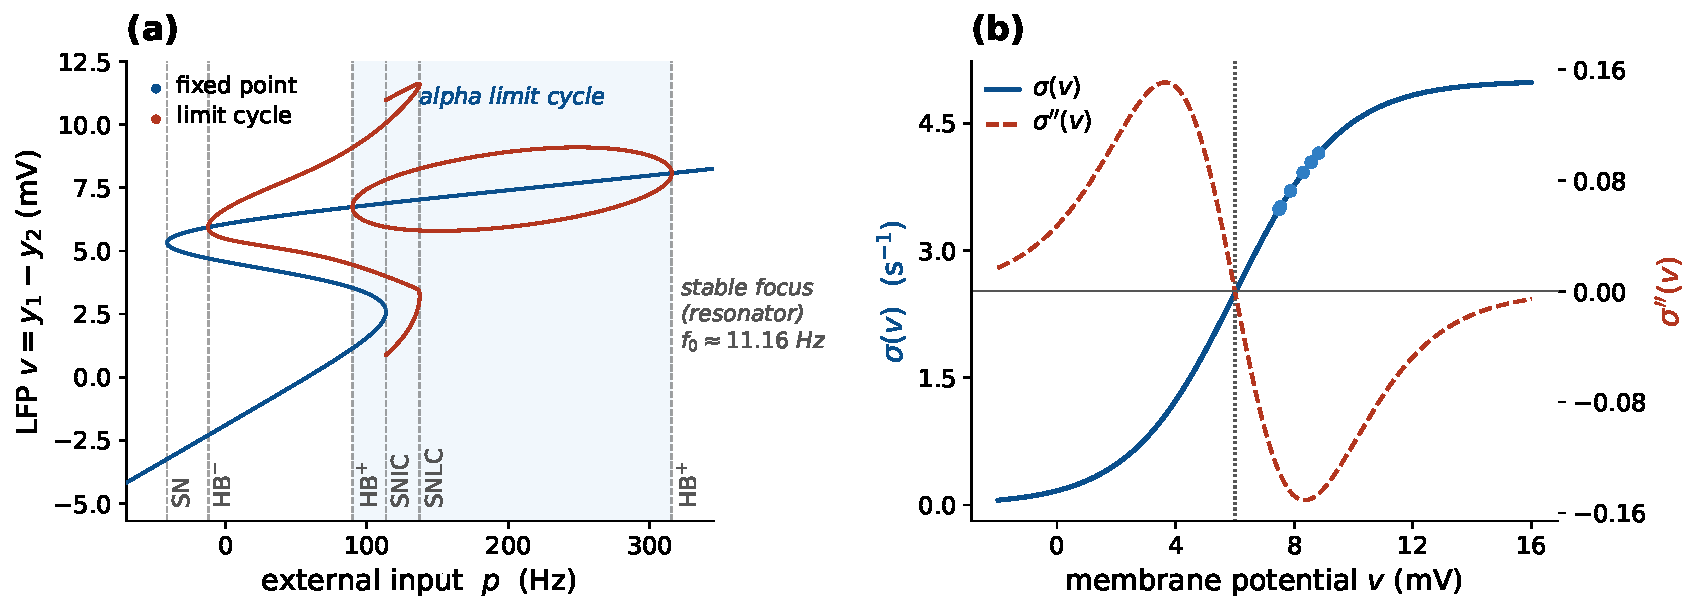
\includegraphics[width=\textwidth]{fig_bifurcation_sigmoid.pdf}
\caption{\DIFdelbeginFL \DIFdelFL{\textbf{The Jansen--Rit operating regime: bifurcation and sigmoid curvature.}
}\DIFdelendFL \DIFaddbeginFL \DIFaddFL{\textbf{JR operating states and sigmoid curvature.}
}\DIFaddendFL \emph{(a)} \DIFdelbeginFL \DIFdelFL{JR bifurcation diagram from numerical continuation---the LFP $v=y_1-y_2$ along
the fixed-point branch }\DIFdelendFL \DIFaddbeginFL \DIFaddFL{Numerical continuation of fixed points }\DIFaddendFL (blue) and \DIFdelbeginFL \DIFdelFL{the min/max of the limit-cycle branches }\DIFdelendFL \DIFaddbeginFL \DIFaddFL{cycle extrema
}\DIFaddendFL (red) \DIFdelbeginFL \DIFdelFL{vs.\
}\DIFdelendFL \DIFaddbeginFL \DIFaddFL{against }\DIFaddendFL external \DIFdelbeginFL \DIFdelFL{input }\DIFdelendFL \DIFaddbeginFL \DIFaddFL{drive }\DIFaddendFL $p$\DIFdelbeginFL \DIFdelFL{, with \emph{solid} }\DIFdelendFL \DIFaddbeginFL \DIFaddFL{; solid branches are }\DIFaddendFL stable\DIFdelbeginFL \DIFdelFL{and \emph{faded} }\DIFdelendFL \DIFaddbeginFL \DIFaddFL{, faded branches
}\DIFaddendFL unstable. The alpha \DIFdelbeginFL \DIFdelFL{limit
}\DIFdelendFL cycle \DIFdelbeginFL \DIFdelFL{(shaded) }\DIFdelendFL lies between \DIFdelbeginFL \DIFdelFL{the }\DIFdelendFL Hopf points \DIFdelbeginFL \DIFdelFL{at $p\!\approx\!90$ }\DIFdelendFL \DIFaddbeginFL \DIFaddFL{near $90$ }\DIFaddendFL and
$316$~s$^{-1}$. \DIFdelbeginFL \DIFdelFL{The alpha cycle coexists with a lower stable fixed point up to }\DIFdelendFL \DIFaddbeginFL \DIFaddFL{Beyond }\DIFaddendFL the \DIFdelbeginFL \DIFdelFL{saddle-node on
an invariant circle (SNIC, $p\!\approx\!114$), then with a large-amplitude cycle up
to its saddle-node near $p=137$. The SNIC terminates the large-amplitude branch,
not the alpha cycle.
At the }\DIFdelendFL upper Hopf \DIFdelbeginFL \DIFdelFL{, $f_0\!\approx\!11.16$~Hz; beyond it }\DIFdelendFL the fixed point is a stable focus,
\DIFdelbeginFL \DIFdelFL{the near-Hopf resonator used here}\DIFdelendFL \DIFaddbeginFL \DIFaddFL{with $f_0\approx11.16$~Hz}\DIFaddendFL . \DIFdelbeginFL \DIFdelFL{Further
codim-1 points are marked }\DIFdelendFL \DIFaddbeginFL \DIFaddFL{Markers identify saddle-nodes }\DIFaddendFL (\DIFdelbeginFL \DIFdelFL{saddle-node }\DIFdelendFL SN\DIFaddbeginFL \DIFaddFL{)}\DIFaddendFL , Hopf \DIFaddbeginFL \DIFaddFL{points
(}\DIFaddendFL HB\DIFdelbeginFL \DIFdelFL{$^{\pm}$}\DIFdelendFL \DIFaddbeginFL \DIFaddFL{$^\pm$)}\DIFaddendFL , \DIFaddbeginFL \DIFaddFL{the }\DIFaddendFL saddle-node \DIFaddbeginFL \DIFaddFL{on an invariant circle (SNIC), and the
saddle-node }\DIFaddendFL of limit cycles \DIFaddbeginFL \DIFaddFL{(}\DIFaddendFL SNLC).
\emph{(b)} \DIFdelbeginFL \DIFdelFL{The sigmoid $\Sig(v)$ }\DIFdelendFL \DIFaddbeginFL \DIFaddFL{Sigmoid }\DIFaddendFL and \DIFdelbeginFL \DIFdelFL{its }\DIFdelendFL curvature\DIFdelbeginFL \DIFdelFL{$\Sig''(v)$, which sets the
demodulation gain and vanishes at the inflection $v_0$. Dots }\DIFdelendFL \DIFaddbeginFL \DIFaddFL{; dots }\DIFaddendFL mark the \DIFaddbeginFL \DIFaddFL{modeled }\DIFaddendFL operating points\DIFdelbeginFL \DIFdelFL{reached by the closed-loop model for the $p$ values used here}\DIFdelendFL .}
\label{fig:bif}
\end{figure}

We compare the \emph{open-loop detector}, the firing-rate sigmoid at a fixed
operating point $v^*$ without recurrence, with the \emph{closed-loop} column, the full recurrent
Jansen--Rit with its feedback. The open-loop detector passes the two-tone field through
$\Sig$ at $v^*$ and applies Eq.~\eqref{eq:lockin}, isolating the pure demodulation law\DIFdelbegin \DIFdel{(Figs.~\ref{fig:carrier},~\ref{fig:opp},~\ref{fig:khz})}\DIFdelend ; its signed in-phase
component $L_{\cos}$ verifies the curvature law, including its sign.
\DIFdelbegin \DIFdel{The \emph{bifurcation
diagram} records the }\DIFdelend \DIFaddbegin \DIFadd{Simulation checks of the continuation diagram record }\DIFaddend field-free min/max of $v$
\DIFdelbegin \DIFdel{vs.\ }\DIFdelend \DIFaddbegin \DIFadd{against }\DIFaddend $p$, \DIFdelbegin \DIFdel{each run initialized at its }\DIFdelend \DIFaddbegin \DIFadd{initialized at the }\DIFaddend fixed point plus a small kick. The \emph{two-dimensional map} evaluates
$A_\Omega$ over an ($\Omega,p$) grid. We verify the mechanism three ways: the
square law ($A_\Omega$ vs.\ $\varepsilon$ on a well-damped focus, expecting a
log--log slope of $2$); a linearization control (replacing $\Sig$ in
the pyramidal sigmoid \DIFdelbegin \DIFdel{of App.~\ref{app:models}, }\DIFdelend \DIFaddbegin \DIFadd{in }\DIFaddend Eq.~\eqref{eq:jr0} \DIFdelbegin \DIFdel{, }\DIFdelend by its tangent at $v^*$, which must abolish the $\Omega$
response); and a check of $\Sig',\Sig''$ against finite differences. Code and reproduction limits are listed under \emph{Code and data availability}.

\subsection{Exact next-generation mean field (NMM2 PING)}\label{sec:nmm2-methods}
The \DIFdelbegin \DIFdel{NMM2 PING}\DIFdelend \DIFaddbegin \DIFadd{pyramidal--interneuron network gamma (PING) }\DIFaddend circuit couples excitatory
and inhibitory MPR populations through
second-order synapses \cite{montbrio2015,ruffini2021nmm2,clusella2023}.
We use the Rosetta Stone formulation \cite{ruffini2025rosetta}, which places this
derived mean field on the same footing as \DIFdelbegin \DIFdel{JR and LaNMM (\S\ref{sec:nmm})}\DIFdelend \DIFaddbegin \DIFadd{the JR and laminar models}\DIFaddend . For
population $X\in\{E,I\}$ (excitatory or inhibitory), $r_X$ is the physical
firing rate (ms$^{-1}$ in the integration), $v_X$ the dimensionless mean QIF
voltage, and $\tau_X$ the membrane time (ms). Dots denote physical-time derivatives:
\begin{equation}
\begin{aligned}
\tau_E\dot r_E&=\Delta/(\pi\tau_E)+2r_Ev_E, &\quad
\tau_E\dot v_E&=v_E^2+\bar\eta-(\pi\tau_E r_E)^2+\tau_E J\,(r_E^{\rm syn}-r_I^{\rm syn})+I_E(t),\\[2pt]
\tau_I\dot r_I&=\Delta/(\pi\tau_I)+2r_Iv_I, &\quad
\tau_I\dot v_I&=v_I^2+\bar\eta-(\pi\tau_I r_I)^2+\tau_I J\,(r_E^{\rm syn}-2r_I^{\rm syn}),
\end{aligned}
\label{eq:nmm2-ping}
\end{equation}
with second-order synaptic activations $r_E^{\rm syn}=\hat K_a[r_E]$ (excitatory, time constant
$\tau_a$) and $r_I^{\rm syn}=\hat K_g[r_I]$ (inhibitory, $\tau_g$), each obeying the same
critically damped operator as the JR synapse, $\tau_s^2\ddot r_{\rm syn}+2\tau_s\dot r_{\rm syn}+r_{\rm syn}=r$; here $J$
is the dimensionless global synaptic gain and the relative weights $(w_{EE},w_{EI},w_{IE},w_{II})=(1,1,1,2)$
use target $X$ and source $Y$ in $w_{XY}$\DIFdelbegin \DIFdel{and set the E and I rows: the $E$ membrane sees $J\,(r_E^{\rm syn}-r_I^{\rm syn})$ and the $I$ membrane
$J\,(r_E^{\rm syn}-2r_I^{\rm syn})$, the only asymmetry being the
doubled $I\!\to\!I$ weight }\DIFdelend \DIFaddbegin \DIFadd{. The only weight asymmetry is the
doubled inhibitory self-coupling, }\DIFaddend $w_{II}=2$.

\DIFaddbegin \DIFadd{In the schematic, $\mathcal U_j(t)$ is the total synaptic and field input
to QIF neuron $j$, and $J^*$ denotes a coupling-induced Hopf.
}\DIFaddend The common background drive $\bar\eta$ is the bifurcation parameter: raising it
past a supercritical Hopf at $\bar\eta_H=1.110$ opens a gamma limit cycle (the gamma
counterpart of the JR alpha Hopf). The applied field enters the excitatory voltage equation
as a current-like forcing, $I_E(t)=\lambda_I E(t)$ in the convention of the exact mean field
\cite{ruffini2021nmm2}, with instantaneous field-to-current coupling $\lambda_I$, as two genuine tones at
$f_c\mp\Delta f/2$ (carrier $f_c=300$~Hz, envelope $\Delta f$ swept through the gamma band)
of current amplitude $A_f$ in the dimensionless MPR drive units, the same
normalization as $\bar\eta$. Thus $\lambda_I$ is measured in normalized drive per V/m. The E membrane $\tau_E\dot v_E$
integrates this forcing into the carrier-frequency excursion $A_f/(\omega\tau_E)$ that the
exact quadratic $v_E^2$ term rectifies, with no postulated sigmoid; the PING as run
therefore computes membrane access with $\tau_m=\tau_E$.

We integrate with fixed-step RK4 ($\Delta t=0.05$~ms) and read out the lock-in
(Eq.~\eqref{eq:lockin}) of $r_E$ at $\Delta f$ over the $(\Delta f, \bar\eta)$ plane.
Parameters (Rosetta Stone PING \cite{ruffini2025rosetta}): $\Delta=1$, global coupling
$J=15$, $\tau_E=15$, $\tau_I=7.5$, $\tau_a=10$, $\tau_g=2.5$~ms, with $\bar\eta$ swept
through the supercritical Hopf at $\bar\eta_H=1.110$ ($f_0=54.0$~Hz), located by bisection
on the leading eigenvalue of the mean-field Jacobian. The simulations retain these
finite membrane times; Eq.~\eqref{eq:slow_synapse} characterizes the fast-membrane limit.

As in JR, either background drive or coupling can bring the circuit to its Hopf.
The resonance map sweeps $\bar\eta$ (Fig.~\ref{fig:nmm2_map}); the coupling sweep,
called the J-curve, varies
$J$ at fixed $\bar\eta$ toward $J^*$, located by bisection on the leading
Jacobian eigenvalue, and reads the lock-in peak of $r_E$ over $\Delta f$
(Fig.~\ref{fig:nmm2_jcurve}). Unlike the JR J-curve, this sweep does not pin the
operating point. At $\bar\eta=0$, we track the eigenpair that reaches the Hopf by
continuation and define $\gamma$ from that critical pair, even where another mode
dominates the response. The linear reference includes the operating-state
dependence of the carrier response and the recurrent transfer. We compute its
second-order source from the PING quadratic terms at the central carrier,
$300$~Hz, and apply the full linearized network response over $15$--$90$~Hz
in $0.025$~Hz steps. Using the distinct AM sidebands changes the peak gain by
less than $0.1\%$ across this sweep.

The simulated coupling sweep uses the AM surrogate, $A_f=8$, with $5$~s
settling and a $4$~s window. We search around each linear resonance, extending
the frequency grid until each sampled maximum is bracketed, and compare
amplitudes $A_f=2,4,8$ at nine couplings. Local parabolic interpolation changes
the sampled peaks by less than $1.3\%$. The figure scales the linear reference
to the median measured gain over $14.5<J<16$; the amplitude check instead
normalizes peak response divided by $A_f^2$ and linear gain to its value at
$A_f=2$, $J=15.53$. These normalizations compare gain variation with the detector coefficient
allowed to vary along this unpinned sweep.

\DIFdelbegin \DIFdel{We check the stability }\DIFdelend \DIFaddbegin \DIFadd{Stability }\DIFaddend of the driven \DIFdelbegin \DIFdel{$J$-curve endpoint by integrating the full
variational matrix along its trajectory. At carrier $300$~Hz and beat $50.5$~Hz,
the AM input repeats every $2$~s. After $8$~s of settling, we compute the
perturbation
multipliersover that period and repeat over the next period.
Moduli below one indicate decay of perturbations to the periodic response.
Two-tone controls at $J=16.5663$ and $16.5901$, both with a $50.5$~Hz beat,
use $5$~s settling, }\DIFdelend \DIFaddbegin \DIFadd{endpoint is checked using period-to-period perturbation
multipliers, }\DIFaddend direct perturbation decay, and \DIFdelbegin \DIFdel{an $8$~s }\DIFdelend \DIFaddbegin \DIFadd{a }\DIFaddend finite-time Lyapunov estimate\DIFdelbegin \DIFdel{.
}\DIFdelend \DIFaddbegin \DIFadd{;
settings and results are given in supplement, \S\ref{app:ping-stability}.
}\DIFaddend

\DIFdelbegin \DIFdel{Although a DC-only averaged calculation predicts an unstable endpoint, the full
periodically forced solution remains attracting: its largest perturbation
multiplier is $0.034$ over the $2$~s forcing period. Increasing settling from
$0.6$ to $3$~s changes the endpoint lock-in by $0.8\%$. With genuine two tones,
the $50.5$~Hz endpoint control also attracts nearby trajectories: perturbations
decay at $-0.0014$~ms$^{-1}$, and the $8$~s Lyapunov estimate is
$-0.00079$~ms$^{-1}$. These controls test a nonlinear driven response, not linear
gain about the DC-shifted equilibrium.
}\DIFdelend \subsection{QIF spiking network (microscale of NMM2)}\label{sec:qif-methods}
NMM2 is the exact infinite-population mean field of all-to-all QIF neurons
\cite{montbrio2015,ruffini2025rosetta,clusella2023}. We integrate that network directly
to compare beat-locked and ongoing activity at the spike level\DIFdelbegin \DIFdel{(\S\ref{sec:qif})}\DIFdelend : $N=8000$ QIF neurons per
population, parameters identical to the PING mean field (Eq.~\eqref{eq:nmm2-ping}),
with single-neuron voltages $V_j$, finite spike threshold $V_{\rm peak}=100$ and reset $-V_{\rm peak}$ in model
voltage units, excitabilities $\eta_j\sim$ Lorentzian$(\bar\eta,\Delta)$ sampled by deterministic
quantiles, second-order synapses driven by the empirical population rates, and a genuine
two-tone field entering the excitatory membranes. Spiking and threshold dynamics are
where the AM surrogate and the physical waveform cannot be assumed equivalent beyond
perturbation theory, so this run uses two tones throughout.

The common background drive $\bar\eta$ places the field-free mean field below or
above a gamma Hopf at $\bar\eta_H=1.110$ ($f_0=54.0$~Hz). We use
$\bar\eta=0.85$ with a $55$~Hz beat and $\bar\eta=1.5$ with a $42$~Hz beat.
Both runs have carrier $f_c=300$~Hz and amplitude $A_f=35$ per tone. We label the conditions by their field-free state and separate the beat-locked
component from other gamma activity. \DIFdelbegin \DIFdel{The spectra }\DIFdelend \DIFaddbegin \DIFadd{Spectra }\DIFaddend and rate folds \DIFdelbegin \DIFdel{do not by themselves
}\DIFdelend \DIFaddbegin \DIFadd{resolve frequency components but do not }\DIFaddend establish
phase capture\DIFdelbegin \DIFdel{(\S\ref{sec:vocab})}\DIFdelend .

We also run both conditions at $A_f=10$ per tone with the same measurement
settings. For $\bar\eta=0.85$, separate checks double the population size,
double the measurement window, or halve the integration step; further runs raise
$V_{\rm peak}$ to $200$ and $400$ at both time steps. An equal-RMS
mean-field control replaces the two tones by one $300$~Hz carrier with peak
amplitude $\sqrt{2}A_f$, using the same duration: both inputs have mean-square
amplitude $A_f^2$ over these windows. The carrier comparison starts from the
field-free equilibrium and uses $800$~ms settling and $800$~ms measurement,
with a $3200$~ms window to check spectral leakage at the larger amplitude.

For two nearby carriers, the fast-carrier approximation gives a constant shift
of the excitatory drive, $\delta\eta_E\simeq A_f^2/(\omega_c\tau_E)^2$, from the
quadratic voltage term. We refine this estimate using the full PING linear carrier
responses and their second-order DC source, then solve for the carrier-averaged
equilibrium and its stability, including the source's dependence on that equilibrium.
This approximation isolates the mean shift; direct two-tone integrations retain
the beat forcing and provide a separate check.

The network is integrated with Euler steps of $0.0025$~ms, settled for $800$~ms (over
four field-free relaxation times at $\bar\eta=0.85$, where the mean-field relaxation time is
$176$~ms) and measured over an integer number of beat cycles, $44$ at $55$~Hz and $34$ at
$42$~Hz ($800$ and $810$~ms), removing the phase-coverage bias from incomplete
beat cycles. Envelope-locked timing is quantified by the quadrature lock-in $A_\Omega$ of
$r_E(t)$ at $\Delta f$, reported as the modulation depth $A_\Omega/\langle r_E\rangle$ (a
stable measure; the off$\to$on lock-in ratio would divide by the field-free floor), and
per neuron by the pairwise phase consistency of each neuron's spike phases at $\Delta f$
(PPC; \cite{vinck2010}), which is unbiased in the spike count, over neurons with at least ten
spikes in the window.

\DIFdelbegin \DIFdel{At $A_f=10$ }\DIFdelend \DIFaddbegin \DIFadd{Weak-drive beat depth remains cutoff-sensitive, }\DIFaddend and \DIFdelbegin \DIFdel{$\bar\eta=0.85$, the finite-network beat depth is $0.093$
for the published cutoff, versus the mean-field value $0.128$. Raising the spike cutoff from $V_{\rm peak}=100$ to
$200$ and $400$ gives depths $0.127$ and $0.139$, while the mean-rate increase
stays at $2.8$--$2.9\%$. At the original cutoff, doubling the population gives
$0.083$ and halving the time step gives $0.093$. The response is therefore
sensitive to the finite spike cutoff. Halving the step at cutoffs $200$ and
$400$ gives depths $0.121$ and $0.141$, respectively: cutoff dependence persists,
and quantitative convergenceremains unestablished at this population size. At the plotted cutoff, the pooled }\DIFdelend \DIFaddbegin \DIFadd{population-size and time-step
checks do not establish joint convergence. At stronger drive, }\DIFaddend spike-phase
\DIFdelbegin \DIFdel{vector strength is $0.046$;
median per-neuron phase consistency remains negative in field-off and field-on
windows at all three cutoffs.
In the $A_f=35$ convergence checks, halving the time step changes the lock-in and the pooled vector
strength by under $1\%$; doubling the spike-detection threshold changes the lock-in by
about $1\%$ and the mean rate by $2\%$, but the pooled vector strength at
$\bar\eta=0.85$ by about $45\%$, so phase concentration, unlike rate modulation
, is sensitive to
how spike times are defined}\DIFdelend \DIFaddbegin \DIFadd{concentration remains more cutoff-sensitive than rate modulation
(supplement, \S\ref{app:qif-checks})}\DIFaddend .

\subsection{Coupling sweeps, timing, and the tACS control (Jansen--Rit)}
The \DIFdelbegin \DIFdel{coupling sweeps of Figs. ~\ref{fig:jcurve} and~\ref{fig:timing}, and the transcranial
alternating-current stimulation (tACS) control of Fig.~\ref{fig:tacs}, use the single JR
column with the field-free operating point $v^*$ pinned: for
each
global }\DIFdelend \DIFaddbegin \DIFadd{JR sweeps vary coupling while keeping detection fixed. For each
}\DIFaddend connectivity $C$\DIFdelbegin \DIFdel{we solve the field-free fixed-point relation analytically
}\DIFdelend \DIFaddbegin \DIFadd{, we solve }\DIFaddend for the external drive $p(C)$ that holds \DIFdelbegin \DIFdel{$v^*$ (hence $\Sig''(v^*)$) fixed, vary $C$
toward the
alpha Hopf, and read $\gamma,\omega_0$ from the $6\times6$ Jacobian. The field
is }\DIFdelend the
\DIFaddbegin \DIFadd{field-free voltage at $v^*=8.30$~mV, then obtain damping and modal frequency
from the Jacobian. This fixes the background curvature without canceling
stimulation-induced mean shifts.
}

\DIFadd{The gain sweep uses the }\DIFaddend AM surrogate\DIFdelbegin \DIFdel{of Eq.~\eqref{eq:amsur} for Fig.~\ref{fig:jcurve}, genuine two
tones for }\DIFdelend \DIFaddbegin \DIFadd{; }\DIFaddend the timing comparison \DIFdelbegin \DIFdel{(Fig.~\ref{fig:timing}), or a direct in-band sinusoid $s(t)=\varepsilon\cos\Omega t$
($\varepsilon=0.1$~mV) for the tACS control (Fig.~\ref{fig:tacs}), each read out by the
lock-in of $v$ at $\Delta f$, except in the timing comparison, which reads the
}\DIFdelend \DIFaddbegin \DIFadd{uses genuine
two tones and measures }\DIFaddend modulation and mean of the same pyramidal rate
$r_P=\Sig(v+s)$. \DIFdelbegin \DIFdel{That comparison uses $18$~s settling and a $20$~s window for each waveform.
The Figure~\ref{fig:jcurve}--Figure~\ref{fig:tacs} response-ratio comparison uses
$v^*=8.30$~mV, TI surrogate amplitude $0.3$~mV with $m=1$ }\DIFdelend \DIFaddbegin \DIFadd{The tACS control uses a direct sinusoid at the same beat
frequency and reads the same voltage lock-in as TI. Further controls match
tACS to TI's generated beat source }\DIFaddend and \DIFdelbegin \DIFdel{$f_c=100$~Hz,
and tACS amplitude $0.1$~mV, driven at each field-free modal frequency.
The original TI amplitudes are interpolated logarithmically in $C$ onto the tACS
grid. For the waveform comparison, both the surrogate and two-tone TIare rerun
on that grid with $12$~s settling and a $6$~s window. Pinning fixes the background curvature; it does not cancel the stimulation-induced
mean shift.
Additional controls at $C=110$, $133.9091$, and $136.3$ use a tACS amplitude of
$0.0143039$~mV, matched to the leading TIbeat source. They record mean voltage,
mean rate, and lock-in with $12$~s settling and a $6$~s window, repeated with
$60$~s settling and a $20$~s window; the latter settings also test genuine two tones. }\DIFdelend \DIFaddbegin \DIFadd{repeat the comparison with longer
settling and measurement windows. Waveforms, amplitudes, and run windows
are recorded together in the supplement.
}\DIFaddend

\DIFdelbegin \subsection{\DIFdel{Vocabulary: forced response, entrainment, and gating}}%DIFAUXCMD
\addtocounter{subsection}{-1}%DIFAUXCMD
%DIFDELCMD < \label{sec:vocab-methods}
%DIFDELCMD < %%%
\DIFdel{\emph{Forced response} denotes the component driven at the beat $\Delta f$, quantified by the lock-in amplitude (Eq.~\eqref{eq:lockin}). A purely forced regime
requires a stable operating state under stimulation; being below Hopf with the field
off is insufficient. \emph{Entrainment} is reserved for its
dynamical-systems meaning, frequency capture of a \emph{self-sustained} oscillator
\cite{pikovsky2001}; in the maps we screen for it with the dominance criterion
$|f_{\rm out}-\Delta f|<0.3$~Hz on the dominant output frequency. This identifies
frequency dominance, not phase capture. \emph{Gating} is amplitude modulation of a persisting rhythm without
frequency capture \cite{canolty2010,tort2010}. Capture and gating are dynamically different, and the same word would otherwise cover
both. The QIF rate fold measures beat-locked firing, which does not by itself
establish gating of gamma amplitude. Appendix~\ref{sec:vocab} gives the metrics
and the frequency-dominance protocol.
}%DIFDELCMD <

%DIFDELCMD < %%%
\DIFdel{The coupling sweeps approach the Hopf from field-free stable foci ($\gamma>0$), so the
$1/\gamma$ law concerns forced susceptibility. The frequency-dominance maps on
the oscillatory side describe a different observable: their bands broaden with
drive, but an Arnold tongue describes phase capture of the autonomous limit
cycle and requires phase tracking (\S\ref{sec:vocab}).
}%DIFDELCMD <

%DIFDELCMD < %%%
\DIFdelend \section{Results}
\DIFdelbegin \DIFdel{The Jansen--Rit column and the exact next-generation mean field (NMM2) both generate a
difference-frequency component and amplify it near a Hopf bifurcation. The former uses
a memoryless sigmoid; the latter derives the nonlinearity from QIF dynamics. Their
detector coefficients differ, but both separate beat generation from recurrent gain.
Coupling controls that gain at fixed generated drive in the JR column
(\S\ref{sec:jcurve}), and resonance amplifies beat-locked modulation more strongly than
the mean rate (\S\ref{sec:timing}).
The TI/tACS comparison then isolates their
shared amplifier (\S\ref{sec:tacs-results}), before the NMM2 and QIF results
connect dynamic mixing and gain to spikes and field-induced gamma. The laminar
two-band column extends the analysis to carriers of $25$--$80$~Hz and drives up to
$3$~mV (App.~\ref{app:lanmm}).
}%DIFDELCMD <

%DIFDELCMD < %%%
\DIFdelend \subsection{The \DIFdelbegin \DIFdel{Jansen--Rit sigmoid demodulates: an alpha line from a carrier-only input}\DIFdelend \DIFaddbegin \DIFadd{JR column generates and resonantly amplifies the beat}\DIFaddend }
An input containing only the two tones $f_c\mp\Delta f/2$ produces an output
oscillation at their $11.1$~Hz beat, near the column's alpha resonance
(Fig.~\ref{fig:bif}). The alpha peak is absent from the input spectrum
(Fig.~\ref{fig:demod}).

\begin{figure}[t!]
\centering
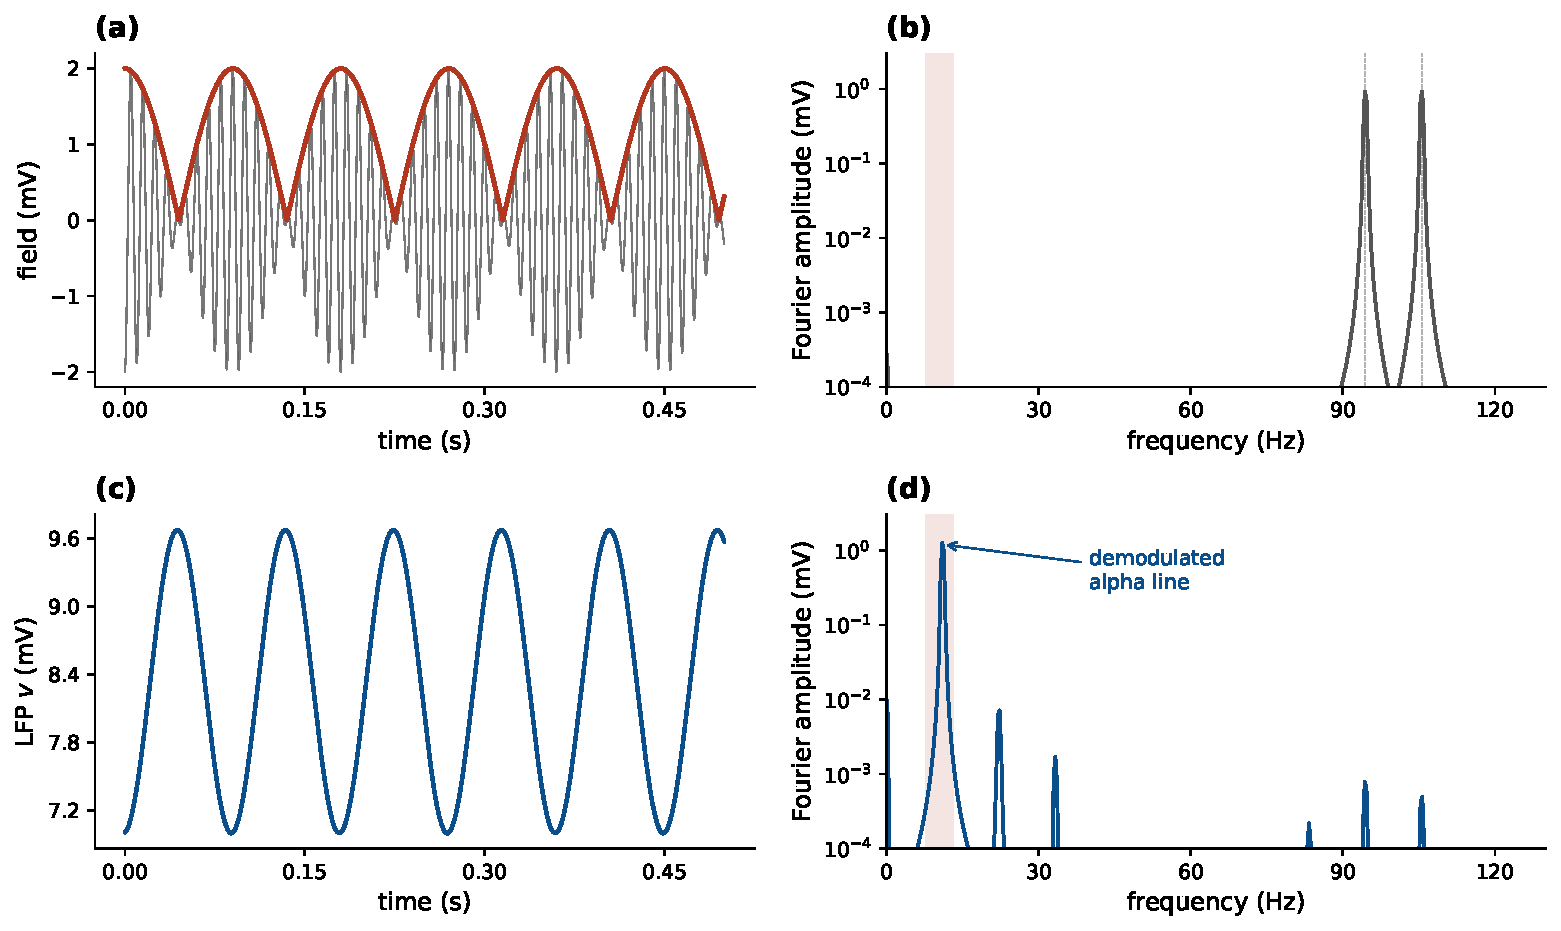
\includegraphics[width=\textwidth]{fig_demodulation_twotone.pdf}
\caption{\DIFdelbeginFL \DIFdelFL{\textbf{An alpha rhythm is synthesized from a two-tone TI input (Jansen--Rit
below Hopf).} The field is the physical TI waveform, two }\DIFdelendFL \DIFaddbeginFL \DIFaddFL{\textbf{The JR column generates a beat absent from the input.}
\emph{(a)} Two }\DIFaddendFL equal tones at \DIFdelbeginFL \DIFdelFL{$f_{1,2}=f_c\mp\Delta f/2$, not the amplitude-modulated surrogate. \emph{(a)} The field
$s(t)$ }\DIFdelendFL \DIFaddbeginFL \DIFaddFL{$94.45$ }\DIFaddendFL and \DIFdelbeginFL \DIFdelFL{its }\DIFdelendFL \DIFaddbeginFL \DIFaddFL{$105.55$~Hz and their }\DIFaddendFL envelope\DIFdelbeginFL \DIFdelFL{$\mathcal A(t)=2\varepsilon|\cos(\Omega t/2)|$---a rectified cosine}\DIFdelendFL ,
\DIFdelbeginFL \DIFdelFL{not a
sinusoid; it is $\mathcal A^2$ that is sinusoidal at $\Omega$ (\S\ref{sec:envelope})}\DIFdelendFL \DIFaddbeginFL \DIFaddFL{$2\varepsilon|\cos(\Omega t/2)|$}\DIFaddendFL . \emph{(b)} \DIFdelbeginFL \DIFdelFL{The input amplitude }\DIFdelendFL \DIFaddbeginFL \DIFaddFL{Input }\DIFaddendFL spectrum\DIFdelbeginFL \DIFdelFL{has lines }\DIFdelendFL \DIFaddbeginFL \DIFaddFL{: }\DIFaddendFL only \DIFdelbeginFL \DIFdelFL{at $f_1$ and $f_2$ ($94.45$ and
$105.55$~Hz, $\Delta f=11.1$~Hz) and no third line at }\DIFdelendFL the \DIFdelbeginFL \DIFdelFL{carrier; in the alpha band
(shaded) it }\DIFdelendFL \DIFaddbeginFL \DIFaddFL{two
tones are present. The alpha-band floor }\DIFaddendFL is $1.6\times10^{-8}$ of \DIFdelbeginFL \DIFdelFL{the tone }\DIFdelendFL \DIFaddbeginFL \DIFaddFL{their
}\DIFaddendFL amplitude, \DIFaddbeginFL \DIFaddFL{from }\DIFaddendFL finite-window leakage\DIFdelbeginFL \DIFdelFL{rather than
physical power}\DIFdelendFL . \DIFdelbeginFL \DIFdelFL{\emph{(c)} }\DIFdelendFL \DIFaddbeginFL \DIFaddFL{\emph{(c,d)} }\DIFaddendFL The \DIFdelbeginFL \DIFdelFL{output }\DIFdelendFL \DIFaddbeginFL \DIFaddFL{synaptic voltage
}\DIFaddendFL $v=y_1-y_2$ \DIFdelbeginFL \DIFdelFL{oscillates at the envelope frequency.
\emph{(d)} The output }\DIFdelendFL \DIFaddbeginFL \DIFaddFL{and its }\DIFaddendFL spectrum \DIFdelbeginFL \DIFdelFL{has a strong peak at }\DIFdelendFL \DIFaddbeginFL \DIFaddFL{show }\DIFaddendFL the \DIFdelbeginFL \DIFdelFL{beat, }\DIFdelendFL \DIFaddbeginFL \DIFaddFL{generated }\DIFaddendFL $11.1$~Hz \DIFdelbeginFL \DIFdelFL{,
synthesized by the sigmoid and absent from the input}\DIFdelendFL \DIFaddbeginFL \DIFaddFL{beat}\DIFaddendFL .
\DIFaddbeginFL \DIFaddFL{The field-free column is a stable focus near its alpha Hopf.}\DIFaddendFL }
\label{fig:demod}
\end{figure}

\DIFdelbegin \subsection{\DIFdel{Near the Hopf, the demodulated beat drives a sharp resonance}}
%DIFAUXCMD
\addtocounter{subsection}{-1}%DIFAUXCMD
\DIFdelend In the stable-focus regime ($p>p_H$), the response is approximately Lorentzian
and its peak grows from $0.23$ to $0.43$ to $0.70$~mV toward the Hopf
(Fig.~\ref{fig:res}), as expected from the
$1/\gamma$ susceptibility. Without a drive the focus is silent at $\Omega$;
the nonlinearity generates that component and recurrence amplifies it.
\DIFaddbegin \DIFadd{The peak shifts with the driven operating state; the near-Hopf law gives
its leading gain, not its exact frequency. The coupling sweep tests that law
over a decade of damping.
}\DIFaddend On the alpha branch below $p_H$, the column free-runs at $f_0$, so the lock-in
can contain both driven and autonomous activity. The dominant output frequency
$f_{\rm out}$ then identifies a frequency-dominance region
(Fig.~\ref{fig:entrain}), without establishing phase capture.

\begin{figure}[t!]
\centering
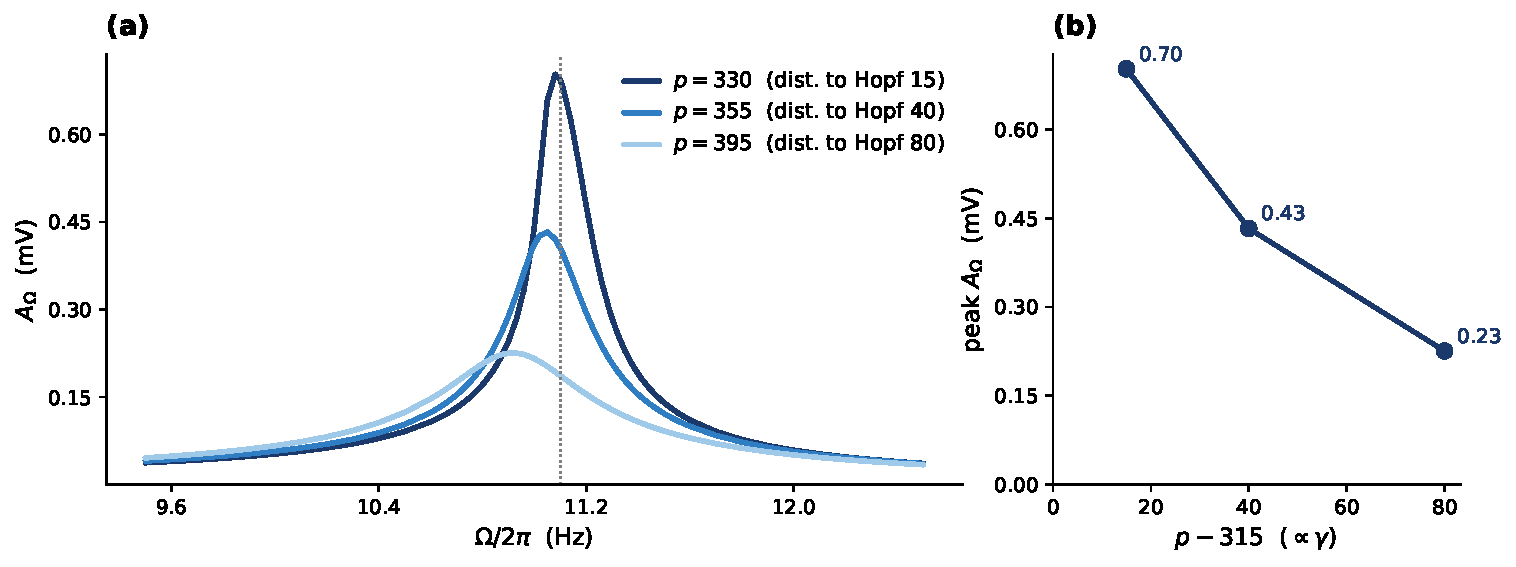
\includegraphics[width=\textwidth]{fig_resonance.pdf}
\caption{\DIFdelbeginFL \DIFdelFL{\textbf{The demodulated beat drives a resonance that sharpens toward the Hopf (Jansen--Rit).}
Fixed-point regime ($p>p_H$, stable focus): lock-in }\DIFdelendFL \DIFaddbeginFL \DIFaddFL{\textbf{The JR beat resonance sharpens toward the Hopf.}
Stable-focus }\DIFaddendFL response at \DIFdelbeginFL \DIFdelFL{$\Omega$ vs.\ envelope
frequency (}\DIFdelendFL $\varepsilon=0.3$~mV\DIFdelbeginFL \DIFdelFL{)}\DIFdelendFL . \emph{(a)} \DIFdelbeginFL \DIFdelFL{The demodulated drive forces an approximately Lorentzian
resonance near $f_0\!\approx\!11.2$~Hz. The measured }\DIFdelendFL \DIFaddbeginFL \DIFaddFL{Lock-in amplitude
against beat frequency; the }\DIFaddendFL finite-amplitude peak \DIFdelbeginFL \DIFdelFL{shifts
}\DIFdelendFL \DIFaddbeginFL \DIFaddFL{moves }\DIFaddendFL from $11.08$ to
$10.93$~Hz across the curves\DIFdelbeginFL \DIFdelFL{as the operating state changes;
Eq}\DIFdelendFL . \DIFdelbeginFL \DIFdelFL{~\eqref{eq:gain} describes its near-Hopf scaling, not its exact location.
The response carries no power at $\Omega$ in the absence of drive, so this is
forced gain. }\DIFdelendFL \emph{(b)} \DIFdelbeginFL \DIFdelFL{The peak height grows }\DIFdelendFL \DIFaddbeginFL \DIFaddFL{Peak amplitude increases }\DIFaddendFL as \DIFaddbeginFL \DIFaddFL{$p$
approaches }\DIFaddendFL the \DIFaddbeginFL \DIFaddFL{upper }\DIFaddendFL Hopf \DIFdelbeginFL \DIFdelFL{is
approached ($p\to p_H$ }\DIFdelendFL from above\DIFdelbeginFL \DIFdelFL{)}\DIFdelendFL . \DIFdelbeginFL \DIFdelFL{Three }\DIFdelendFL \DIFaddbeginFL \DIFaddFL{These three }\DIFaddendFL points \DIFdelbeginFL \DIFdelFL{cannot establish a power
law}\DIFdelendFL \DIFaddbeginFL \DIFaddFL{show sharpening
and growth}\DIFaddendFL ; the \DIFaddbeginFL \DIFaddFL{coupling sweep quantifies the }\DIFaddendFL $1/\gamma$ scaling \DIFdelbeginFL \DIFdelFL{is quantified over a decade, together with }\DIFdelendFL \DIFaddbeginFL \DIFaddFL{and
}\DIFaddendFL its saturation\DIFdelbeginFL \DIFdelFL{, in
Fig}\DIFdelendFL .\DIFdelbeginFL \DIFdelFL{~\ref{fig:jcurve}(c). The above-Hopf regime, with autonomous alpha activity,
is characterized by output frequency in Fig.~\ref{fig:entrain}.}\DIFdelendFL }
\label{fig:res}
\end{figure}

\subsection{Carrier independence and the kHz roll-off}
At fixed post-coupling polarization the demodulated response is flat across the
carrier band, for both the open-loop detector and the closed-loop column near the Hopf
(Fig.~\ref{fig:carrier}). As a function of
the \emph{applied} field, by contrast, the membrane low-pass makes the response roll
off as $1/f_c^2$ above the corner in the point-membrane model
(Fig.~\ref{fig:khz}). Its $16$~ms response gives beat attenuation of about
$10^{-4}$--$10^{-6}$ at $1$--$10$~kHz; the cable-end case in
\DIFdelbegin \DIFdel{App.~\ref{app:access}, Eq.~\eqref{eq:lambda}, }\DIFdelend \DIFaddbegin \DIFadd{the passive-cable calculation }\DIFaddend gives about $10^{-2}$--$10^{-3}$.
The assumed $0.2$~ms point-membrane response retains appreciable carrier access.

\begin{figure}[t!]
\centering
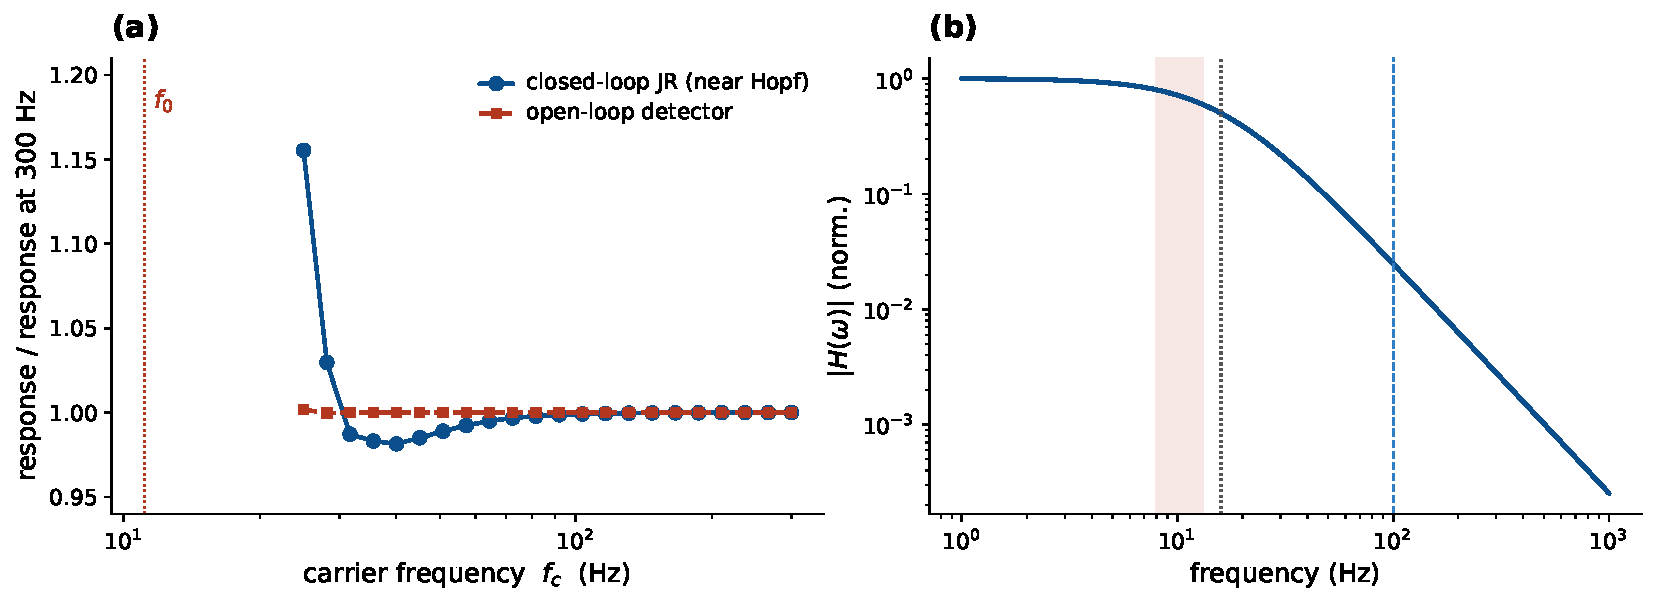
\includegraphics[width=\textwidth]{fig_carrier_independence.pdf}
\caption{\textbf{The demodulated response is carrier-independent at fixed polarization (Jansen--Rit).} \emph{(a)} The demodulated response is
nearly flat across carrier frequency $f_c=25$--$300$~Hz for the open-loop detector
and for the closed-loop JR near the Hopf, with deviations as $f_c$ approaches the
natural band. Each curve is normalized by its own response at $300$~Hz:
$0.00670$~s$^{-1}$ open loop and $0.512$~mV closed loop. Their ratio is a
rate-to-voltage transfer of $76.4$~mV\,s. The open-loop
carrier independence follows to leading order from Eq.~\eqref{eq:demod}. \emph{(b)} The second-order-synapse low-pass $|H_s(\omega)|/|H_s(0)|$
passes the envelope ($\sim$0.7) and suppresses the $100$~Hz carrier ($\sim$2.5\%). Dotted line: synaptic corner $a/2\pi\!\approx\!16$~Hz; shaded band: envelope ($8$--$13$~Hz); dashed line: $100$~Hz carrier.}
\label{fig:carrier}
\end{figure}

We also drive the full recurrent column with a kHz field, passing it through
an explicit membrane low-pass (an extra first-order state, time constant $\tau$) for
each modeled compartment before its polarization reaches the sigmoid. The
column demodulates and resonates at the recovered alpha in the fast-access case
($\tau=0.2$~ms), as
Eq.~\eqref{eq:khz} predicts (Fig.~\ref{fig:khz_direct}a). With two genuine tones centered at $2$~kHz and beating at $10.914$~Hz, the output
contains the beat absent from the input (Fig.~\ref{fig:khz_twotone}); the analytic
access factor is $|H_m|^2=0.137$ for $\tau=0.2$~ms. This quantifies the fast-access
hypothesis under the specified response time and coupling.

\subsection{The nonlinearity is the detector: the
\texorpdfstring{$\Sig''$}{sigma''} curvature law and its controls}\label{sec:results-curvature}
The signed open-loop response tracks $\half\Sig''(v^*)\varepsilon^2 m$ across the
operating range, vanishing and reversing sign at the inflection $v_0$
(Fig.~\ref{fig:opp})---demodulation is the sigmoid-curvature term of
Eq.~\eqref{eq:demod}, and the closed-loop operating points sit where $\Sig''$ is large and negative.
\DIFaddbegin \DIFadd{Changing its sign reverses the source phase; at matched network susceptibility,
its magnitude sets the same resonant-gain calculation on either flank.
}\DIFaddend

\begin{figure}[t!]
\centering
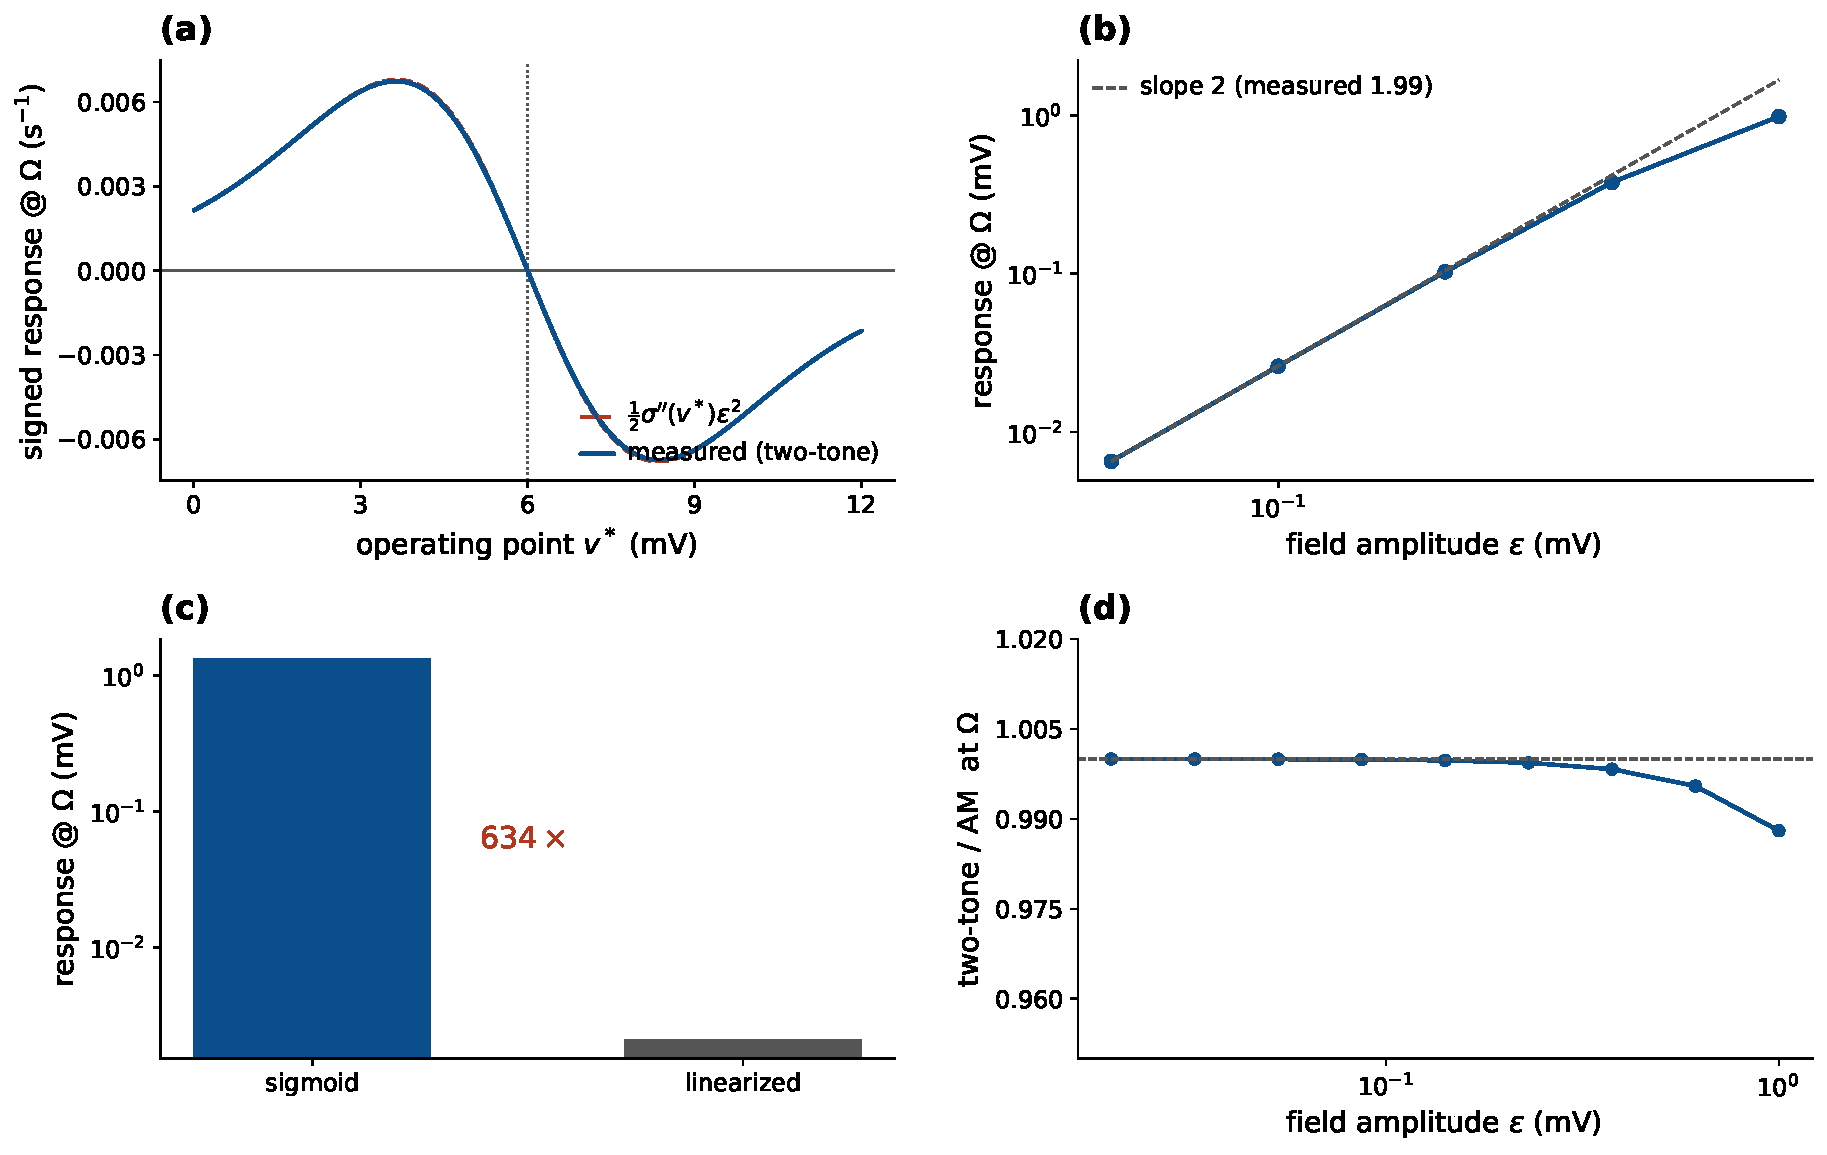
\includegraphics[width=\textwidth]{fig_curvature_twotone.pdf}
\caption{\DIFdelbeginFL \DIFdelFL{\textbf{The curvature law, the square law, and the surrogate control
(Jansen--Rit, genuine two tones).} }\DIFdelendFL \DIFaddbeginFL \DIFaddFL{\textbf{Curvature determines the JR detector.}
}\DIFaddendFL \emph{(a)} The signed open-loop \DIFdelbeginFL \DIFdelFL{response tracks
$\half\Sig''(v^*)\varepsilon^2$ across the operating range (maximum deviation }\DIFdelendFL \DIFaddbeginFL \DIFaddFL{beat follows
$\Sig''(v^*)\varepsilon^2/2$ within }\DIFaddendFL $0.9\%$\DIFdelbeginFL \DIFdelFL{)}\DIFdelendFL , vanishing \DIFdelbeginFL \DIFdelFL{at the inflection $v_0$ }\DIFdelendFL and reversing sign
\DIFdelbeginFL \DIFdelFL{across it}\DIFdelendFL \DIFaddbeginFL \DIFaddFL{at $v_0$}\DIFaddendFL . \DIFdelbeginFL \DIFdelFL{The mechanism is
sign-agnostic: $\Sig''$ sets sign and phase while $|\Sig''|$ sets gain, so the resonance
picture is unchanged up to an overall sign in the $\Sig''>0$ lobe, which this sweep spans.
The sign flip is itself a prediction (\S\ref{sec:predictions}). }\DIFdelendFL \emph{(b)} The \DIFdelbeginFL \DIFdelFL{closed-loop
}\DIFdelendFL \DIFaddbeginFL \DIFaddFL{recurrent }\DIFaddendFL response \DIFdelbeginFL \DIFdelFL{scales as $\varepsilon^2$, measured }\DIFdelendFL \DIFaddbeginFL \DIFaddFL{has amplitude }\DIFaddendFL slope $1.99$.
\emph{(c)} \DIFdelbeginFL \DIFdelFL{Replacing }\DIFdelendFL \DIFaddbeginFL \DIFaddFL{Linearizing }\DIFaddendFL the \DIFdelbeginFL \DIFdelFL{field-receiving }\DIFdelendFL \DIFaddbeginFL \DIFaddFL{receiving }\DIFaddendFL sigmoid \DIFdelbeginFL \DIFdelFL{by its tangent collapses }\DIFdelendFL \DIFaddbeginFL \DIFaddFL{reduces }\DIFaddendFL the \DIFdelbeginFL \DIFdelFL{response $634\times$}\DIFdelendFL \DIFaddbeginFL \DIFaddFL{beat $634$-fold}\DIFaddendFL .
\emph{(d)} \DIFdelbeginFL \DIFdelFL{Surrogate control: the }\DIFdelendFL \DIFaddbeginFL \DIFaddFL{Open-loop }\DIFaddendFL two-tone/AM \DIFaddbeginFL \DIFaddFL{beat }\DIFaddendFL ratio at \DIFdelbeginFL \DIFdelFL{$\Omega$ approaches $1$ as
$\varepsilon\!\to\!0$ (}\DIFdelendFL \DIFaddbeginFL \DIFaddFL{$v^*=8$~mV:
}\DIFaddendFL $1.0000$ at $0.02$~mV \DIFdelbeginFL \DIFdelFL{, }\DIFdelendFL \DIFaddbeginFL \DIFaddFL{and }\DIFaddendFL $0.988$ at $1$~mV\DIFdelbeginFL \DIFdelFL{) for the open-loop
detector at $v^*=8$~mV}\DIFdelendFL . This checks the leading
local source\DIFdelbeginFL \DIFdelFL{; it does }\DIFdelendFL \DIFaddbeginFL \DIFaddFL{, }\DIFaddendFL not \DIFdelbeginFL \DIFdelFL{validate
}\DIFdelendFL the \DIFaddbeginFL \DIFaddFL{nonlinear }\DIFaddendFL recurrent \DIFdelbeginFL \DIFdelFL{AM-surrogate sweeps of Fig.~\ref{fig:jcurve} }\DIFdelendFL \DIFaddbeginFL \DIFaddFL{response }\DIFaddendFL near the Hopf.}
\label{fig:opp}
\end{figure}

In the recurrent column, the response scales quadratically at small drive
(log--log slope $1.99$, measured as in \S\ref{sec:transduction-methods}),
and linearizing the field-receiving sigmoid reduces it
from $1.34$ to $0.0021$~mV (Fig.~\ref{fig:opp}b,c). The open-loop surrogate
comparison in panel~(d) supports its use for leading-order beat sweeps, with
the waveform and near-Hopf limitations specified in \S\ref{sec:waveforms}.

\subsection{Realistic-head comparison of envelope and quadratic maps}\label{sec:fem-results}
Changing the current ratio moves the envelope and mean-square foci in opposite
directions in this head model, while the quadratic beat map only rescales.
Figure~\ref{fig:fem} compares the three maps of Table~\ref{tab:transduction-maps}, the
envelope excursion $\mathcal M[\mathcal A]$, the quadratic excursion
$\mathcal M[\tfrac12\mathcal A^2]$ and the mean-square polarization $\mathcal I$, for
the Violante montage in IXI002. All three use the same local polarizations, along the direction chosen at
1:1 and held fixed (\S\ref{sec:fem-methods}).

\DIFdelbegin \DIFdel{At }\DIFdelend \DIFaddbegin \DIFadd{Table~\ref{tab:fem-summary} summarizes the }\DIFaddend 1:1 \DIFdelbegin \DIFdel{($2+2$~mA) the hippocampal means are $0.16$~mV, $0.018$~mV$^2$ and
$0.0094$~mV$^2$, respectively. The target-to-reference ratio is $1.22$ for the envelope
map, $1.17$ for the quadratic excursion ($1.08$ degree-matched) and $0.92$ for
$\mathcal I$ ($0.96$). Once degree is matched, the quadratic map therefore favors the
hippocampus less than the envelope map does, as Eq.~\eqref{eq:reweight} predicts where
the dominant local polarization is larger in the reference than at the target;
$\mathcal I$ favors the reference.
}%DIFDELCMD <

%DIFDELCMD < %%%
\DIFdel{Changing the current ratio separates the three maps (Fig.~\ref{fig:fem}a--c,f). From
1:1 }\DIFdelend to 1:3 \DIFaddbegin \DIFadd{change. The pair-current
product falls from $4$ to $3$~mA$^2$, so }\DIFaddend the quadratic excursion \DIFdelbegin \DIFdel{is multiplied by
$I_1^{\rm pair}I_2^{\rm pair}/(2~\mathrm{mA})^2=0.75$ }\DIFdelend \DIFaddbegin \DIFadd{falls to $75\%$
of its value }\DIFaddend at every node, to machine precision. Its normalized map, \DIFdelbegin \DIFdel{its target-to-reference ratio and its focus
do not change:
this is the fixed-state product law of \S\ref{sec:envelope}}\DIFdelend \DIFaddbegin \DIFadd{contrast, and focus
are unchanged}\DIFaddend . The envelope focus moves \DIFdelbegin \DIFdel{$2.5$~mm anteriorly($2.2$--$4.0$~mm over the 5--50\% fractions)}\DIFdelend \DIFaddbegin \DIFadd{anteriorly}\DIFaddend , toward the pair whose current
falls\DIFdelbegin \DIFdel{. Its ratio drops from $1.22$ to $0.95$, and its hippocampal mean falls by
45\%. The focus of $\mathcal I$ moves $4.5$~mm posteriorly($2.4$--$8.2$~mm)}\DIFdelend \DIFaddbegin \DIFadd{; the mean-square focus moves posteriorly}\DIFaddend , toward the pair whose current rises.
\DIFdelbegin \DIFdel{Its hippocampal mean rises by 24\%, while its ratio
changes little (}\DIFdelend \DIFaddbegin \DIFadd{At 1:1, degree matching reduces the quadratic contrast to $1.08$, below the
envelope's $1.22$, while mean-square polarization favors the reference.
}

\begin{table}[htbp]
\centering\small
\caption{\DIFaddFL{\textbf{Hippocampal maps under current-ratio changes.} Means refer to the
ROI; contrasts are ROI/reference 95th-percentile ratios. Parentheses give
square-root, degree-matched contrasts. Focus shifts use the top 10\% of ROI
nodes, with anterior positive; ranges over other fractions are supplementary.}}
\label{tab:fem-summary}
\begin{tabular}{@{}lrrrrr@{}}
\toprule
\DIFaddFL{Map }& \DIFaddFL{Mean, 1:1 }& \DIFaddFL{Contrast, 1:1 }& \DIFaddFL{Contrast, 1:3 }& \DIFaddFL{Mean change }& \DIFaddFL{Focus shift}\\
\midrule
\DIFaddFL{Envelope }& \DIFaddFL{$0.16$ mV }& \DIFaddFL{$1.22$ }& \DIFaddFL{$0.95$ }& \DIFaddFL{$-45\%$ }& \DIFaddFL{$+2.5$ mm}\\
\DIFaddFL{Quadratic beat }& \DIFaddFL{$0.018$ mV$^2$ }& \DIFaddFL{$1.17$ ($1.08$) }& \DIFaddFL{$1.17$ ($1.08$) }& \DIFaddFL{$-25\%$ }& \DIFaddFL{$0$ mm}\\
\DIFaddFL{Mean square }& \DIFaddFL{$0.0094$ mV$^2$ }& \DIFaddendFL $0.92$ \DIFdelbeginFL \DIFdelFL{to $0.90$) .
}\DIFdelendFL \DIFaddbeginFL \DIFaddFL{($0.96$) }& \DIFaddFL{$0.90$ }& \DIFaddFL{$+24\%$ }& \DIFaddFL{$-4.5$ mm}\\
\bottomrule
\end{tabular}
\end{table}
\DIFaddend

The sweep shows two kinds of steering (Fig.~\ref{fig:fem}e,f). The envelope ratio peaks
near balance ($1.24$ at a posterior share of $0.525$) and falls to $0.89$--$0.94$ at
the extremes. Its focus moves only while the two carriers are comparable inside the
hippocampus. At a posterior share of $0.6$ or more, the anterior pair is the weaker
carrier at more than 96\% of hippocampal nodes; at $0.4$ or less, the posterior pair is. The
envelope map then equals twice the weaker pair's polarization over most of the ROI,
and its measured focus changes little with further imbalance. The focus of $\mathcal I$ moves
continuously instead, from $1.5$~mm anterior at a posterior share of $0.1$ to $6.3$~mm
posterior at $0.9$, while its ratio stays between $0.79$ and $0.94$ ($0.89$--$0.97$
degree-matched). The quadratic excursion keeps one ratio and one focus across the
whole sweep.

The isotropic beat map (Fig.~\ref{fig:fem}d,g) has a target-to-reference ratio of $1.18$
($1.08$ degree-matched), close to that of the fixed-direction quadratic map. It also
scales with $I_1^{\rm pair}I_2^{\rm pair}$, so the current ratio cannot steer it either.

\DIFdelbegin \DIFdel{The atlas labellowers the absolute ratios (envelope $1.17$, quadratic excursion $1.04$
at 1:1) but keeps every direction of focus
displacement: envelope }\DIFdelend \DIFaddbegin \DIFadd{Across all 32 combinations of montage, label, tissue definition, and focus
fraction, the envelope shift remains anterior, the mean-square shift posterior,
and the quadratic beat shift zero. Radial projections preserve those directions
but change absolute contrasts more than the atlas label does (supplement,
\S\ref{supp:fem-sensitivities}).
}\ifjne\else
\subsection{\DIFadd{Sensitivity of focus displacement}}\label{supp:fem-sensitivities}
\DIFadd{The spatial ordering in the article persists across montage, labeling, tissue,
and focus-fraction choices. Table~\ref{tab:fem-sensitivities} gives the ranges;
orientation changes absolute contrast more than the atlas label in this subject.
For the reference projection and label, the top-5--50\% focus moves
$2.2$--$4.0$~mm anteriorly for the envelope and $2.4$--$8.2$~mm posteriorly
for mean-square polarization.
}

\begin{table}[htbp]\centering\small
\caption{\DIFaddFL{Focus displacement from 1:1 to 1:3. Envelope shifts are anterior;
mean-square shifts are posterior. The quadratic beat shift is zero in every case.
Contrasts quoted in the last column are raw 1:1 envelope/quadratic contrasts.}}
\label{tab:fem-sensitivities}
\begin{tabular}{@{}lrrl@{}}
\toprule
\DIFaddFL{Sensitivity }& \DIFaddFL{Envelope (mm) }& \DIFaddFL{Mean square (mm) }& \DIFaddFL{Contrasts}\\
\midrule
\DIFaddFL{Atlas label }& \DIFaddendFL $2.0$--$3.8$ \DIFdelbeginFL \DIFdelFL{~mm
anterior, $\mathcal I$ }\DIFdelendFL \DIFaddbeginFL & \DIFaddendFL $3.2$--$5.9$ \DIFdelbeginFL \DIFdelFL{~mm posterior,
quadratic excursion zero. Along the
radial direction the displacements also keep their directions
(envelope }\DIFdelendFL \DIFaddbeginFL & \DIFaddFL{$1.17$ / $1.04$}\\
\DIFaddFL{Radial direction }& \DIFaddendFL $1.9$--$2.8$ \DIFdelbeginFL \DIFdelFL{~mm
anterior, $\mathcal I$ }\DIFdelendFL \DIFaddbeginFL & \DIFaddendFL $2.0$--$3.7$ \DIFdelbeginFL \DIFdelFL{~mm posterior), but the ratios change more than with
the label: }\DIFdelendFL \DIFaddbeginFL & \DIFaddendFL $1.62$ \DIFdelbeginFL \DIFdelFL{for the envelope and }\DIFdelendFL \DIFaddbeginFL \DIFaddFL{/ }\DIFaddendFL $1.97$\DIFdelbeginFL \DIFdelFL{for the quadratic excursion at 1:1. In
this subject the assumed orientation , more than the label, sets the absolute contrast.
Across all }\DIFdelendFL \DIFaddbeginFL \\
\DIFaddFL{All }\DIFaddendFL 32 \DIFdelbeginFL \DIFdelFL{combinations of montage, label, ROI tissue definition and focus fraction,
every envelope shift is anterior (}\DIFdelendFL \DIFaddbeginFL \DIFaddFL{combinations }& \DIFaddendFL $0.7$--\DIFdelbeginFL \DIFdelFL{$8.1$~mm ), every shift of $\mathcal I$ is
posterior (}\DIFdelendFL \DIFaddbeginFL \DIFaddFL{$8.1$ }& \DIFaddendFL $0.5$--$10.6$ \DIFdelbeginFL \DIFdelFL{~mm), and every shift of the quadratic excursion is zero.
}\DIFdelendFL \DIFaddbeginFL & \\
\bottomrule
\end{tabular}
\end{table}
\DIFaddend

\DIFaddbegin \fi

\DIFaddend All four maps are geometric quantities before detector gain. $\mathcal I$ is
nonnegative and does not by itself assign excitation or suppression
(\S\ref{sec:dc}). These results come from one subject and one montage, with
quasi-static conductivities and a uniform coupling.

\begin{figure}[htbp]
\centering
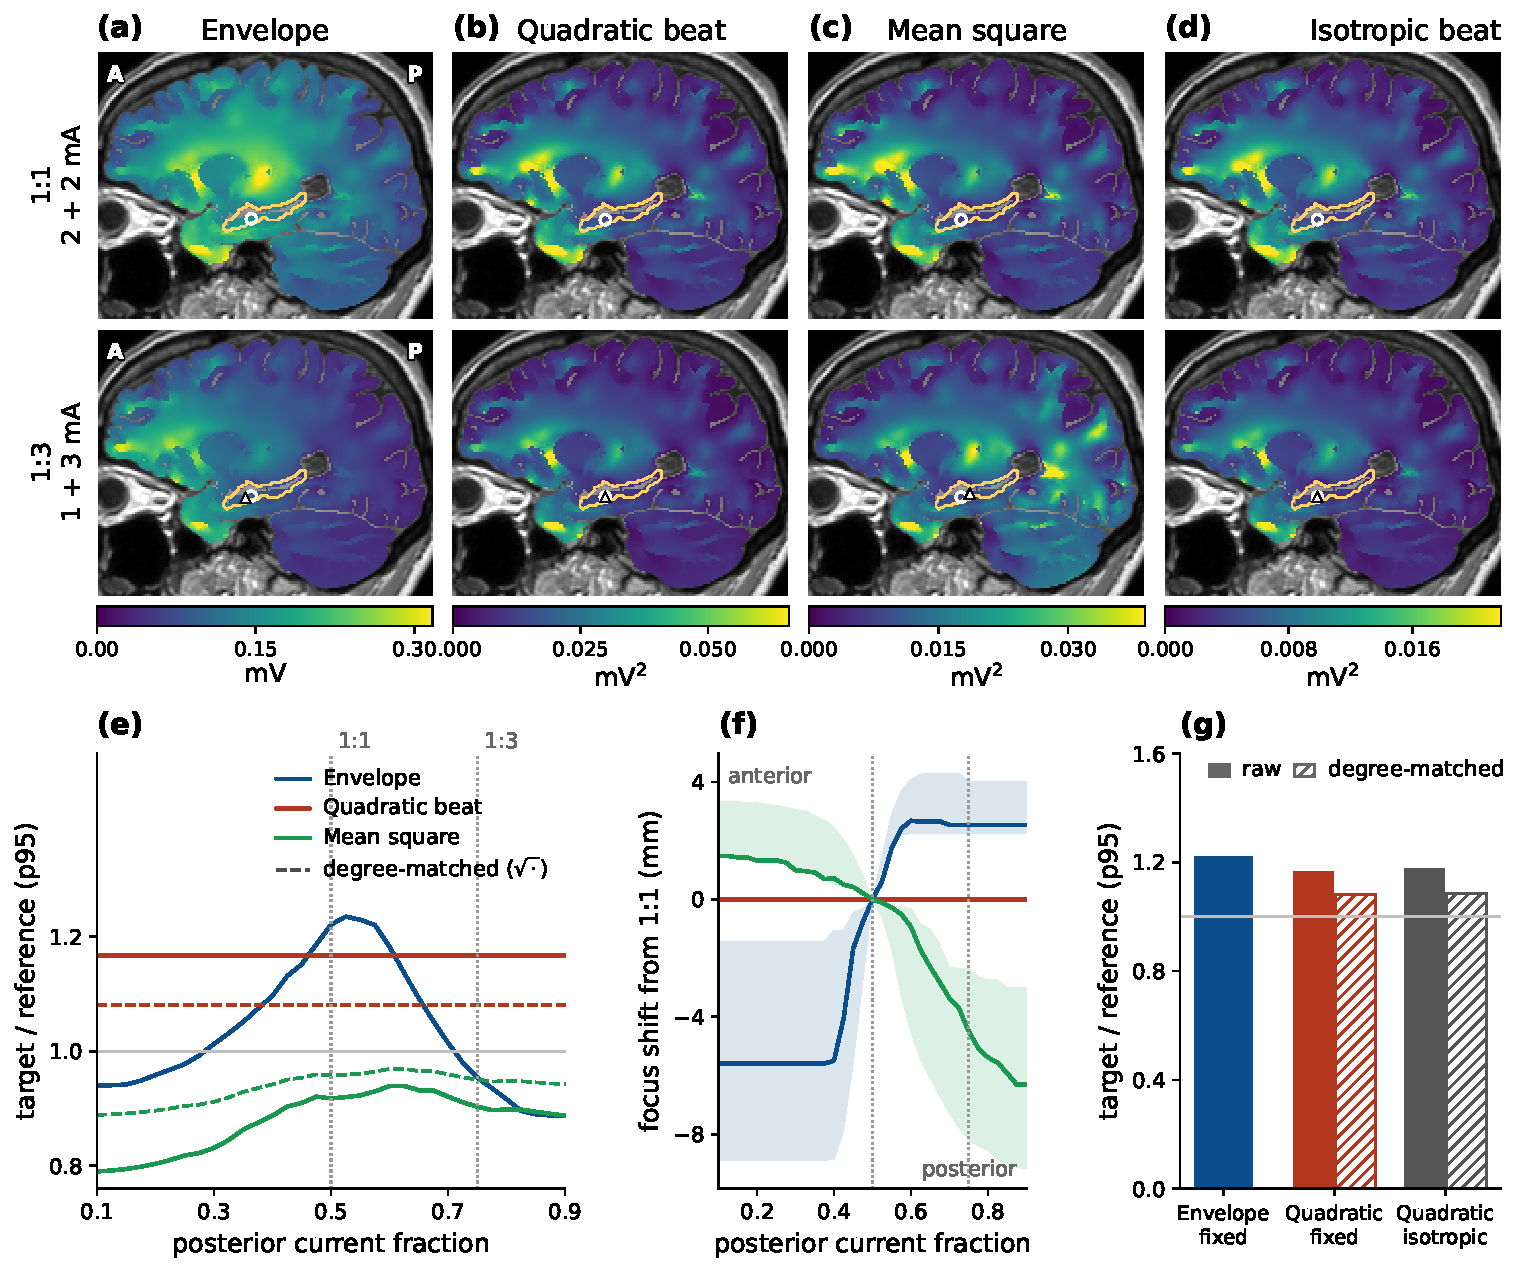
\includegraphics[width=\textwidth]{fig_fem.pdf}
\caption{\DIFdelbeginFL \DIFdelFL{\textbf{Envelope and quadratic maps in a realistic head} (IXI002, }\DIFdelendFL \DIFaddbeginFL \DIFaddFL{\textbf{Envelope and quadratic maps in IXI002.}
}\DIFaddendFL Violante montage\DIFdelbeginFL \DIFdelFL{, FreeSurfer }\DIFdelendFL \DIFaddbeginFL \DIFaddFL{; }\DIFaddendFL left hippocampus outlined in gold\DIFdelbeginFL \DIFdelFL{). \emph{(a--d)} Sagittal plane
through the hippocampal centroid}\DIFdelendFL , anterior to the left\DIFaddbeginFL \DIFaddFL{.
\emph{(a--d)} Sagittal maps at $2+2$~mA (top) and $1+3$~mA (bottom)}\DIFaddendFL :
envelope excursion, quadratic excursion\DIFdelbeginFL \DIFdelFL{and }\DIFdelendFL \DIFaddbeginFL \DIFaddFL{, }\DIFaddendFL mean-square polarization, \DIFdelbeginFL \DIFdelFL{all along the 1:1 envelope-maximizing direction
held fixed, }\DIFdelendFL and
\DIFdelbeginFL \DIFdelFL{the }\DIFdelendFL isotropic beat\DIFdelbeginFL \DIFdelFL{excursion}\DIFdelendFL . \DIFdelbeginFL \DIFdelFL{Top row }\DIFdelendFL \DIFaddbeginFL \DIFaddFL{The first three use the fixed }\DIFaddendFL 1:1 \DIFdelbeginFL \DIFdelFL{($2+2$~mA), bottom row 1:3
(1~mA anterior, 3~mA posterior)}\DIFdelendFL \DIFaddbeginFL \DIFaddFL{envelope-maximizing
direction}\DIFaddendFL . Each \DIFdelbeginFL \DIFdelFL{column has one }\DIFdelendFL color scale \DIFdelbeginFL \DIFdelFL{, from zero to its
gray-matter 99th percentile }\DIFdelendFL \DIFaddbeginFL \DIFaddFL{ends }\DIFaddendFL at \DIFaddbeginFL \DIFaddFL{its }\DIFaddendFL 1:1 \DIFdelbeginFL \DIFdelFL{; $\lambda_0=0.5$~mV per V/m}\DIFdelendFL \DIFaddbeginFL \DIFaddFL{gray-matter 99th percentile}\DIFaddendFL .
Circles \DIFaddbeginFL \DIFaddFL{and triangles }\DIFaddendFL mark the \DIFaddbeginFL \DIFaddFL{projected top-10\% }\DIFaddendFL focus at 1:1 \DIFdelbeginFL \DIFdelFL{(centroid of the top 10\% of hippocampal nodes) }\DIFdelendFL and \DIFdelbeginFL \DIFdelFL{triangles the focus at }\DIFdelendFL 1:\DIFdelbeginFL \DIFdelFL{3,
both projected onto the plane. }\DIFdelendFL \DIFaddbeginFL \DIFaddFL{3.
}\DIFaddendFL \emph{(e)} \DIFdelbeginFL \DIFdelFL{Hippocampal 95th percentile over reference
95th percentile across the ratio sweep, at 4~mA total. Dashed lines are degree-matched
(square root of the second-order }\DIFdelendFL \DIFaddbeginFL \DIFaddFL{Target-to-reference contrast; dashed curves use square-root
}\DIFaddendFL maps \DIFdelbeginFL \DIFdelFL{)}\DIFdelendFL \DIFaddbeginFL \DIFaddFL{to match degree}\DIFaddendFL . \emph{(f)} \DIFdelbeginFL \DIFdelFL{Focus }\DIFdelendFL \DIFaddbeginFL \DIFaddFL{Anterior focus }\DIFaddendFL displacement\DIFdelbeginFL \DIFdelFL{from 1}\DIFdelendFL : \DIFdelbeginFL \DIFdelFL{1 along
the hippocampal long axis, anterior positive: }\DIFdelendFL top 10\%
(line)\DIFdelbeginFL \DIFdelFL{and the }\DIFdelendFL \DIFaddbeginFL \DIFaddFL{, }\DIFaddendFL range over 5--50\% (band). \DIFdelbeginFL \DIFdelFL{The quadratic excursion's displacement is zero at every ratio.
}\DIFdelendFL \emph{(g)} \DIFdelbeginFL \DIFdelFL{Target-to-reference ratio of the envelope and quadratic excursions along the
fixed direction and of the isotropic beat excursion, }\DIFdelendFL \DIFaddbeginFL \DIFaddFL{Contrasts }\DIFaddendFL at 1:1\DIFdelbeginFL \DIFdelFL{; the two beat maps keep
these values at every ratio. Solid bars give raw-map contrasts; }\DIFdelendFL \DIFaddbeginFL \DIFaddFL{, raw
(solid) and degree-matched (}\DIFaddendFL hatched\DIFdelbeginFL \DIFdelFL{bars give
the square-root contrasts for the second-order maps}\DIFdelendFL \DIFaddbeginFL \DIFaddFL{)}\DIFaddendFL .
The \DIFdelbeginFL \DIFdelFL{envelope has one bar
because it is already first order. The }\DIFdelendFL reference is \DIFdelbeginFL \DIFdelFL{all }\DIFdelendFL gray matter outside the \DIFdelbeginFL \DIFdelFL{hippocampal }\DIFdelendFL ROI\DIFdelbeginFL \DIFdelFL{, including other deep gray matter}\DIFdelendFL . All maps \DIFdelbeginFL \DIFdelFL{are geometric, before }\DIFdelendFL \DIFaddbeginFL \DIFaddFL{precede }\DIFaddendFL detector
gain\DIFdelbeginFL \DIFdelFL{; the mean-square polarization
}\DIFdelendFL \DIFaddbeginFL \DIFaddFL{: $\mathcal I$ }\DIFaddendFL weights \DIFdelbeginFL \DIFdelFL{the signed steady rate source $Y_{\rm DC}$ of \S\ref{sec:dc}
and is }\DIFdelendFL \DIFaddbeginFL \DIFaddFL{$Y_{\rm DC}=\Sig''\mathcal I/2$, but does }\DIFaddendFL not \DIFdelbeginFL \DIFdelFL{itself a source}\DIFdelendFL \DIFaddbeginFL \DIFaddFL{set its sign}\DIFaddendFL .}
\label{fig:fem}
\end{figure}

\subsection{Coupling sets the gain at fixed detection}\label{sec:jcurve}
\DIFdelbegin \DIFdel{The resonance sweeps above drove the column toward the Hopf with the external input
$p$, but $p$ also shifts the operating point , entangling detection($\Sig''$) with
amplification. To isolate amplification, we vary the JR global connectivity }\DIFdelend \DIFaddbegin \DIFadd{Changing connectivity at a fixed field-free operating point isolates recurrent
gain from detection. We vary }\DIFaddend $C$ and \DIFdelbegin \DIFdel{solve analytically for the }\DIFdelend \DIFaddbegin \DIFadd{adjust the external }\DIFaddend drive $p(C)$ \DIFdelbegin \DIFdel{that
\emph{pins} the field-free operating point }\DIFdelend \DIFaddbegin \DIFadd{to hold
}\DIFaddend $v^*$, \DIFdelbegin \DIFdel{so the detection gain }\DIFdelend \DIFaddbegin \DIFadd{its curvature }\DIFaddend $\Sig''(v^*)$\DIFaddbegin \DIFadd{, }\DIFaddend and the open-loop \DIFdelbegin \DIFdel{detector amplitude
$A_{\rm open}\simeq\half|\Sig''(v^*)|\varepsilon^2 m$ are held
}\DIFdelend \DIFaddbegin \DIFadd{beat amplitude
$A_{\rm open}\simeq\half|\Sig''(v^*)|\varepsilon^2m$ }\DIFaddend constant. As $C\!\to\!C^*$ (the Hopf, $C^*\!\approx\!137$) the damping
$\gamma\!\to\!0$, the demodulated response grows $\sim30\times$ and the envelope
resonance sharpens (Fig.~\ref{fig:jcurve}a,b), a network effect since
the local detector curvature is fixed while the recurrent transfer changes. Its modal frequency and
input--output projections vary with $C$ as well as its damping. The rate-to-voltage gain
$A_\Omega/A_{\rm open}$ (mV\,s) tracks $1/\gamma$ before saturating near criticality
(Fig.~\ref{fig:jcurve}c); driving the same column to the Hopf through the input $p$
rather than the coupling $C$ gives a similar leading gain--$\gamma$ trend.
Both paths approach a weakly damped mode; their finite-distance gains need not
coincide because the modal projections can differ.

\begin{figure}[t!]
\centering
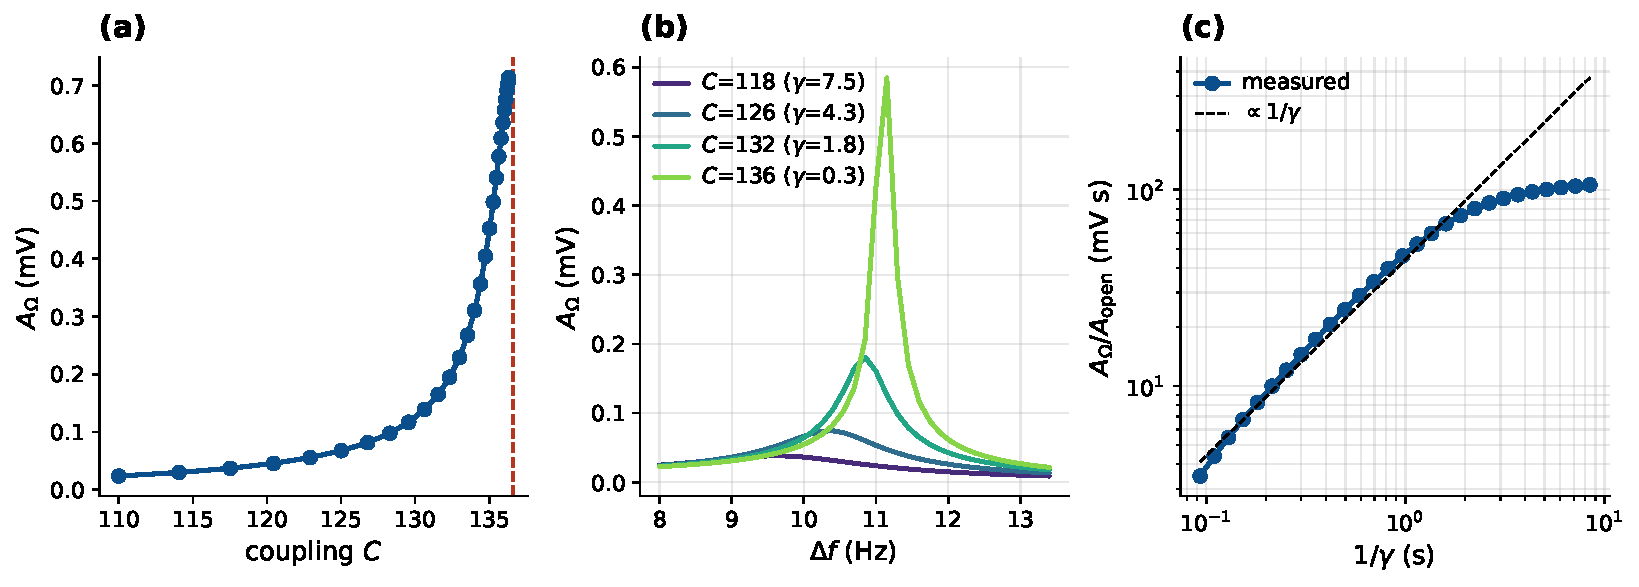
\includegraphics[width=\textwidth]{fig_jcurve.pdf}
\caption{\textbf{Coupling controls the amplification at fixed detection (Jansen--Rit).}
The input is the AM surrogate of Eq.~\eqref{eq:amsur}.
The field-free operating point $v^*$ is pinned by co-solving $p(C)$, so $\Sig''(v^*)=-0.151$~s$^{-1}$mV$^{-2}$ and
$A_{\rm open}$ are held constant throughout. \emph{(a)} The demodulated $A_\Omega$ grows as the
coupling $C$ approaches the Hopf $C^*$ from the stable-focus side ($\gamma>0$). \emph{(b)} The envelope resonance
sharpens and grows as $C\!\to\!C^*$. \emph{(c)} The network gain
$A_\Omega/A_{\rm open}$, in mV\,s, follows $1/\gamma$ (dashed) and saturates near the
bifurcation.}
\label{fig:jcurve}
\end{figure}

\subsection{The resonance amplifies the envelope-locked modulation more than the mean rate}\label{sec:timing}
Pinning $v^*$ to hold the local detector
curvature fixed, as in Fig.~\ref{fig:jcurve}, and driving the column toward the Hopf
through the coupling, we read both quantities from the same observable, the pyramidal
rate $r_P=\Sig(v+s)$ with the field in its argument. With genuine two tones, its
beat-locked modulation at $\Delta f=f_0$ grows $13.2\times$ ($26$ to $339$~mHz),
tracking $1/\gamma$ before saturating; its mean shift grows $4.4\times$ ($-1.8$ to
$-7.7$~mHz), but stays below $0.2\%$ of the $3.9$~Hz baseline
(Fig.~\ref{fig:timing}). The ratio of modulation to mean-shift magnitude rises from
$14.5$ far from the Hopf to $58$ near $\gamma=1$~s$^{-1}$, then falls to $44$ closest
to the Hopf as rectification of the amplified oscillation accelerates the mean shift.
The surrogate \DIFdelbegin \DIFdel{, whose direct DC source is $3/4$ of the two-tone value, gives ratios
of $19$, $66$, and $45$}\DIFdelend \DIFaddbegin \DIFadd{comparison is given in the supplement (\S\ref{supp:waveform-checks})}\DIFaddend . A small mean-rate change can therefore accompany a much
larger beat response in this weakly driven regime, consistent with primate
observations \cite{vieira2024}; both effects are compared in the same rate units.

The demodulator feeds the network a constant term and a line at the beat $\Omega$
(Eq.~\eqref{eq:taylor}), and the transfer $G(\Omega)$ of Eq.~\eqref{eq:gain} treats them
differently: $|G(\omega_0)|\propto1/(2\gamma\omega_0)$ diverges as the Hopf is approached,
while $|G(0)|\propto1/(\omega_0^2+\gamma^2)$ stays finite. This comparison describes
the response to the detector's DC and beat sources. The growing beat response
itself rectifies and contributes another mean shift, quadratic in its amplitude.
Before saturation that contribution can grow as $1/\gamma^2$, so bounded $G(0)$
does not imply a bounded mean shift throughout the approach to the Hopf.

\subsection{TI and tACS share the linear amplifier}\label{sec:tacs-results}
TI and direct low-frequency stimulation share the same linear amplifier.
Matching their generated in-band drives therefore matches their linear outputs;
resonance alone gives TI no efficiency advantage.
For the AM surrogate with amplitude $\varepsilon_{\rm TI}$ and modulation depth
$m$, and a tACS input of amplitude $\varepsilon_{\rm tACS}$, the ratio of voltage
lock-in amplitudes in linear response is
\[
\mathcal R_{\rm lin}
=\frac{|\Sig''(v^*)|\,\varepsilon_{\rm TI}^2m}{2\Sig'(v^*)\,\varepsilon_{\rm tACS}}.
\]
The common network transfer cancels, so the ratio has no dependence on $\gamma$
when both responses are linear about the same state. At the amplitudes used in
Figs.~\ref{fig:jcurve} and~\ref{fig:tacs}, $\mathcal R_{\rm lin}=0.143$.
\DIFdelbegin \DIFdel{The surrogate sweeps give approximately }\DIFdelend \DIFaddbegin \DIFadd{Genuine two tones give output ratios of }\DIFaddend $0.14$ far from the Hopf, \DIFdelbegin \DIFdel{rising to }\DIFdelend $0.24$ at
$\gamma=1.07$~s$^{-1}$\DIFdelbegin \DIFdel{and $0.47$ }\DIFdelend \DIFaddbegin \DIFadd{, and $0.46$ }\DIFaddend at $0.12$~s$^{-1}$. \DIFdelbegin \DIFdel{Genuine two tones give
$0.14$, $0.24$, and $0.46$, respectively, a change of at most $2.2\%$ across the grid}\DIFdelend \DIFaddbegin \DIFadd{The AM-surrogate
comparison is reported in the supplement (\S\ref{supp:waveform-checks})}\DIFaddend .
These are response ratios for the stated unequal input amplitudes, not an
equal-power comparison. \DIFaddbegin \DIFadd{The equal-per-carrier and equal-total-peak comparisons
with both tACS and tDCS are given in \S\ref{sec:dc}.
}\DIFaddend In controls at three couplings, matching the tACS input
to TI's leading beat source gives \DIFaddbegin \DIFadd{two-tone }\DIFaddend TI/tACS output ratios of $0.99$,
\DIFdelbegin \DIFdel{$0.94$, and
$0.92$ for the surrogate, and $0.99$, }\DIFdelend $0.93$, and $0.90$\DIFdelbegin \DIFdel{for two tones.
Increasing that direct input by a factor of }\DIFdelend \DIFaddbegin \DIFadd{.
The stronger direct response saturates earlier near the Hopf: multiplying
its input by }\DIFaddend $6.99$ increases \DIFdelbegin \DIFdel{its response
by }\DIFdelend \DIFaddbegin \DIFadd{the output by only }\DIFaddend $6.97$, $3.95$, and $1.96$
\DIFdelbegin \DIFdel{, respectively. The larger response saturates earlier, with stimulation-induced mean shiftsthat }\DIFdelend \DIFaddbegin \DIFadd{at these three couplings. Stimulation-induced mean shifts, which }\DIFaddend field-free
pinning does not cancel\DIFdelbegin \DIFdel{; this accounts for the finite-amplitude
}\DIFdelend \DIFaddbegin \DIFadd{, account for this }\DIFaddend departure from the linear ratio\DIFdelbegin \DIFdel{near criticality}\DIFdelend .

\subsection{Exact mean-field confirmation: the NMM2 PING gamma generator}\label{sec:nmm2-results}
The exact PING mean field generates and amplifies the beat through its derived
$v_E^2$ nonlinearity. With a $300$~Hz two-tone field entering the excitatory
current, the lock-in of $r_E$ shows a growing gamma resonance below the Hopf
and a response superposed on autonomous gamma above it
(Figs.~\ref{fig:nmm2_res},~\ref{fig:nmm2_map}). The resonance ridge intensifies
through the Hopf; its appreciable frequency shift with operating point makes
it diagonal, unlike the JR sweep shown here \cite{clusella2023}.

This derived detector lies on the fast side of its crossover at $300$~Hz:
carrier voltage excursions mix through $v_E^2$ before the rate reads the result.
For the full eight-state PING (Eq.~\eqref{eq:nmm2-ping}), each high-frequency current
tone of amplitude $I_j$ produces a voltage phasor $I_j/(i\omega_j\tau_E)$.
The $v_E^2$ term therefore supplies a difference-frequency source of magnitude
$I_1I_2/(\tau_E^2\omega_1\omega_2)$ inside the equation for $\tau_E\dot v_E$.
After division by $\tau_E$, this source is propagated through the network
susceptibility at $\Omega$. At four stable operating points, the resulting
response agrees with the full second-order calculation to within $1.1\%$ at
$300$~Hz, $0.1\%$ at $1$~kHz, and $0.03\%$ at $2$~kHz
(Fig.~\ref{fig:crossover}b).

\begin{figure}[t!]
\centering
\DIFaddbeginFL 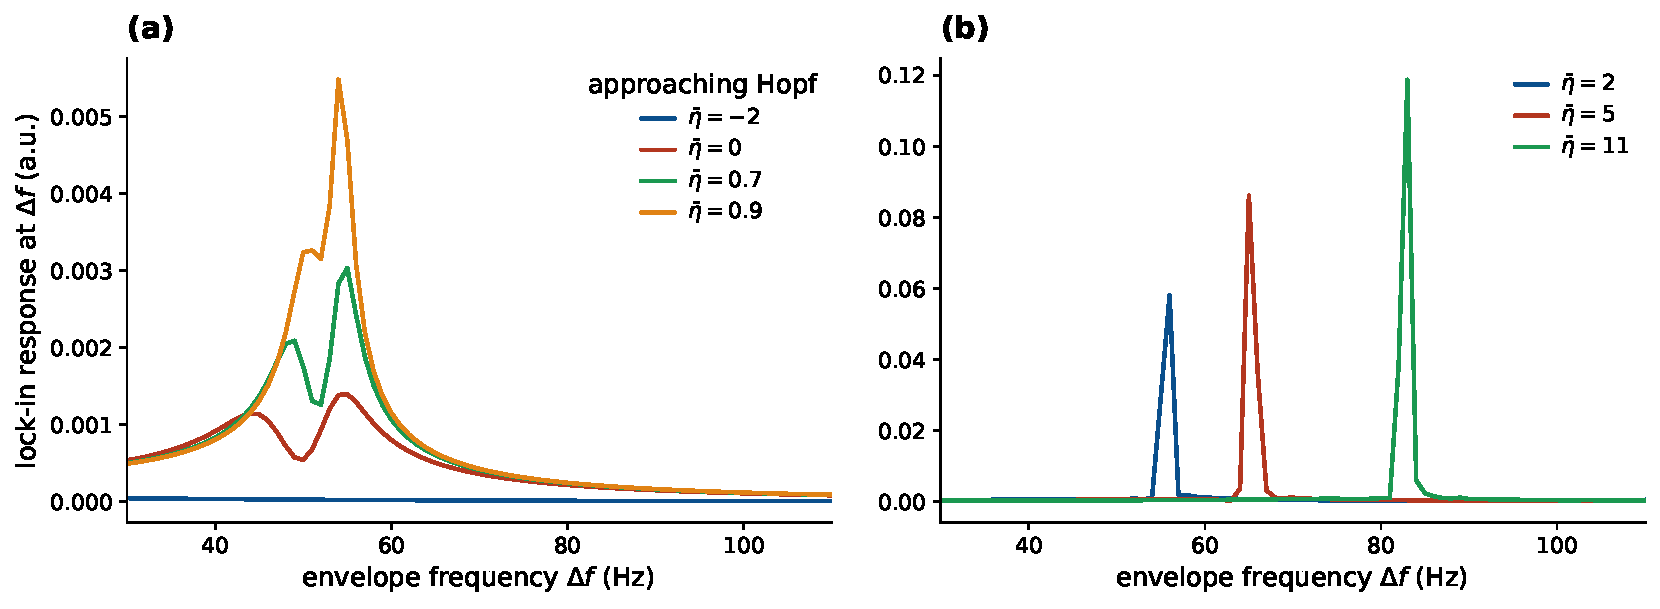
\includegraphics[width=\textwidth]{fig_nmm2_resonance_twotone.pdf}
\caption{\DIFaddFL{\textbf{NMM2 PING gamma resonance (exact mean field, genuine two tones).}
Lock-in response of the excitatory rate $r_E$ at the envelope frequency $\Delta f$ under a
two-tone TI field (carrier $300$~Hz). \emph{(a)} (stable focus,
$\bar\eta<\bar\eta_H=1.110$) forced resonance at the gamma frequency
($f_0\!\approx\!54$~Hz), the peak growing $0.0014\!\to\!0.0030\!\to\!0.0055$~ms$^{-1}$ as the Hopf
is approached ($1/\gamma$ gain). \emph{(b)} (limit cycle,
$\bar\eta>\bar\eta_H$) response in the autonomous-gamma regime, the peak shifting
upward with $\bar\eta$ ($56\!\to\!65\!\to\!83$~Hz). The input carries no power at
$\Delta f$; the response is synthesized by the exact quadratic $v^2$ nonlinearity, with no
sigmoid anywhere in the model. AM/two-tone comparisons are reported in the supplement
(\S\ref{supp:waveform-checks}).}}
\label{fig:nmm2_res}
\end{figure}

\begin{figure}[t!]
\centering
\DIFaddendFL 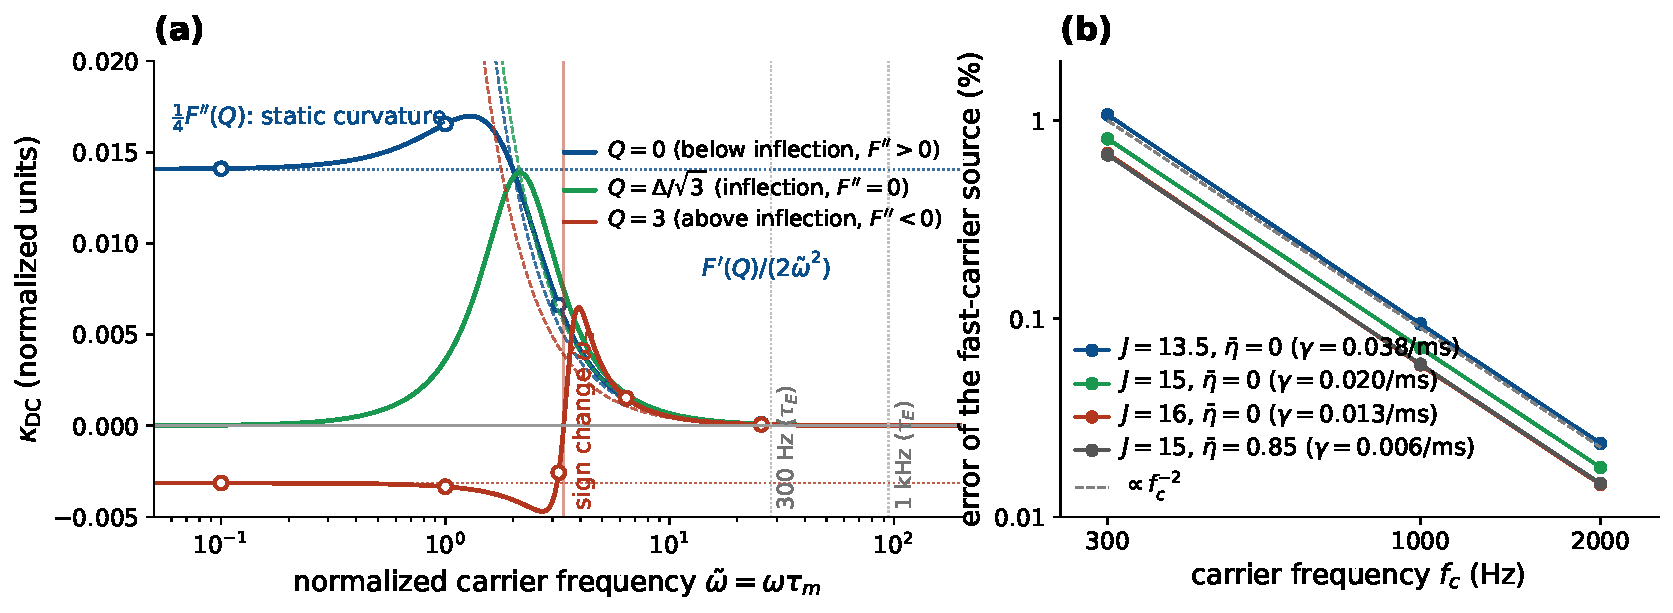
\includegraphics[width=\textwidth]{fig_mpr_crossover.pdf}
\caption{\textbf{Static curvature at slow carriers, slope at fast ones.} \emph{(a)}
Second-order DC rate shift of an uncoupled MPR population ($\Delta=1$\DIFdelbeginFL \DIFdelFL{, dimensionless membrane-time variables}\DIFdelendFL ) under a
current carrier, Eq.~\eqref{eq:crossover}, for operating points below, at and above the
inflection of $F(Q)$. Dotted: the static limit $\tfrac14F''$; dashed: the fast-carrier
limit \DIFdelbeginFL \DIFdelFL{$F'/(2\tilde\omega^2)$}\DIFdelendFL \DIFaddbeginFL \DIFaddFL{$F'/[2(\omega\tau_m)^2]$}\DIFaddendFL ; circles: RK4 integrations at $I_{\rm ac}=0.05$ averaged over whole carrier
periods (relative error below $10^{-3}$). Above the inflection the sign changes \DIFdelbeginFL \DIFdelFL{at
$\tilde\omega_z$}\DIFdelendFL \DIFaddbeginFL \DIFaddFL{with carrier frequency}\DIFaddendFL . The horizontal coordinate is \DIFdelbeginFL \DIFdelFL{$\tilde\omega=\omega\tau_m$}\DIFdelendFL \DIFaddbeginFL \DIFaddFL{$\omega\tau_m$}\DIFaddendFL ; the carrier markers
use $\tau_m=\tau_E=15$~ms. \emph{(b)} PING of Eq.~\eqref{eq:nmm2-ping}: relative error of the
fast-carrier difference-frequency source against the exact second-order response at four
stable operating points ($\gamma$ the damping of the gamma mode), two tones centered at
$300$, $1000$ and $2000$~Hz.}
\label{fig:crossover}
\end{figure}

\DIFdelbegin %DIFDELCMD < \begin{figure}[t!]
%DIFDELCMD < \centering
%DIFDELCMD < 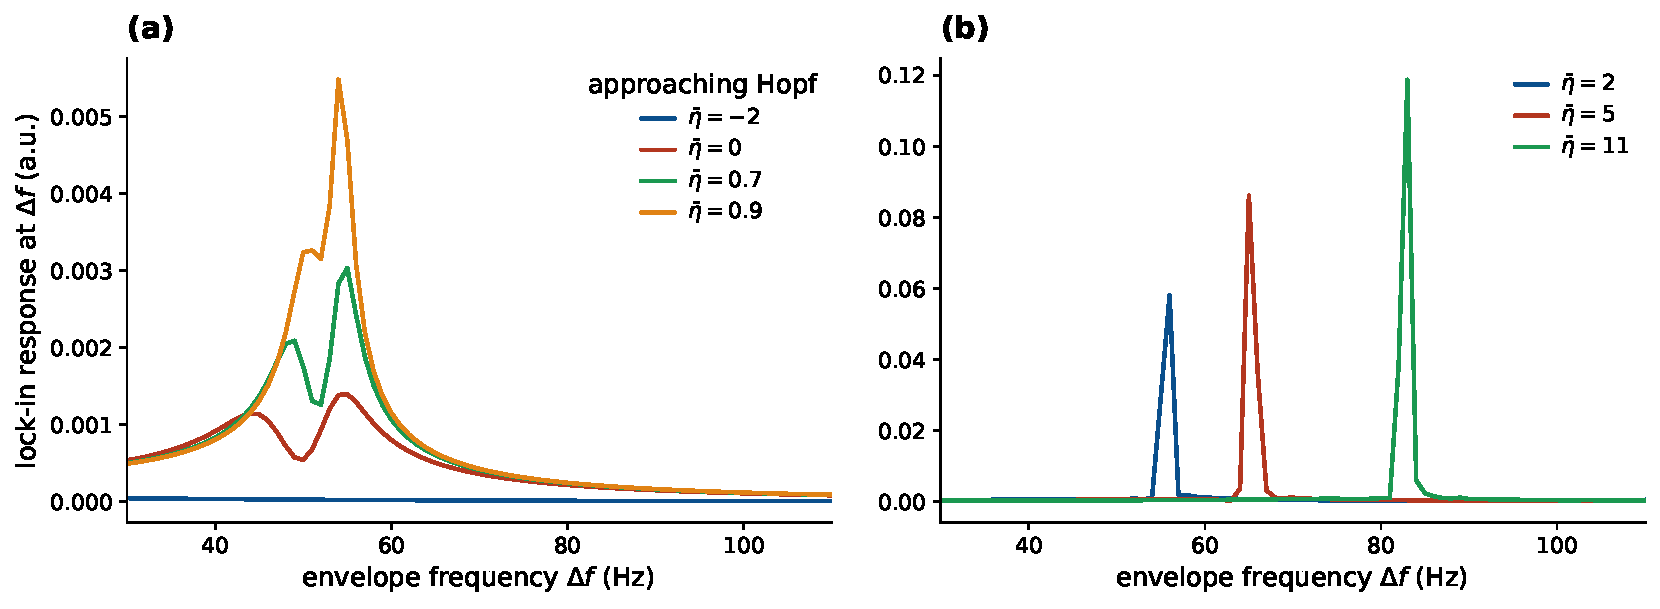
\includegraphics[width=\textwidth]{fig_nmm2_resonance_twotone.pdf}
%DIFDELCMD < \caption{%%%
\DIFdelFL{\textbf{NMM2 PING gamma resonance (exact mean field, genuine two tones).}
Lock-in response of the excitatory rate $r_E$ at the envelope frequency $\Delta f$ under a
two-tone TI field (carrier $300$~Hz). \emph{(a)} (stable focus,
$\bar\eta<\bar\eta_H=1.110$) forced resonance at the gamma frequency
($f_0\!\approx\!54$~Hz), the peak growing $0.0014\!\to\!0.0030\!\to\!0.0055$~ms$^{-1}$ as the Hopf
is approached ($1/\gamma$ gain). \emph{(b)} (limit cycle,
$\bar\eta>\bar\eta_H$) response in the autonomous-gamma regime, the peak shifting
upward with $\bar\eta$ ($56\!\to\!65\!\to\!83$~Hz). The input carries no power at
$\Delta f$; the response is synthesized by the exact quadratic $v^2$ nonlinearity, with no
sigmoid anywhere in the model. Matched AM and two-tone drives agree at $\Omega$ to
$0.07\%$ well below the Hopf and to $4\%$ at $\bar\eta=0.9$, consistent with the JR
surrogate control (Fig.~\ref{fig:opp}d).}%DIFDELCMD < \MBLOCKRIGHTBRACE
%DIFDELCMD < \label{fig:nmm2_res}
%DIFDELCMD < \end{figure}
%DIFDELCMD <

%DIFDELCMD < %%%
\DIFdelend In NMM2 PING, $J$ is the mean inter-neuron QIF synaptic weight.
Sweeping $J$ at fixed background drive toward the gamma Hopf reveals two
competing modes (Fig.~\ref{fig:nmm2_jcurve}). A second mode near $55$~Hz carries
the linear-response peak over $14.6\lesssim J\lesssim16.2$; the critical mode
carries it at lower couplings and again near the Hopf, where its frequency is
about $50$~Hz. In that near-Hopf interval,
$0.0014\lesssim\gamma\lesssim0.0081$~ms$^{-1}$, the linear gain scales as
$1/\gamma$ with a fitted exponent of $1.02$ over a $5.8$-fold damping range.
The full-sweep exponent is $0.71$, so a single-mode law does not describe the
whole curve. \DIFdelbegin \DIFdel{This refines the coupling-controlled sensitivity expected in QIF
networks \cite{clusella2023} : both coupling and rectifier are derived, but the
dominant mode can change}\DIFdelend \DIFaddbegin \DIFadd{Coupling-dependent sensitivity \cite{clusella2023} therefore
includes changes in which mode carries the peak}\DIFaddend .

At $A_f=8$, the simulated response exceeds the normalized linear reference by
up to $48\%$ in the amplitude check, then saturates. At a quarter of that
amplitude ($A_f=2$, one sixteenth of the power), the departures stay within
$11\%$ at the nine tested couplings. The \DIFdelbegin \DIFdel{normalization and endpoint-stability checks are given in
\S\ref{sec:nmm2-methods};
$\gamma$ always describes the field-free critical mode, not the driven state}\DIFdelend \DIFaddbegin \DIFadd{driven endpoint remains attracting under both waveforms
(supplement, \S\ref{app:ping-stability})}\DIFaddend .
The alpha JR and gamma NMM2 circuits share the $1/\gamma$ gain scaling of their critical mode despite their different
mixers, with amplification adjustable through coupling.

\subsection{QIF responses distinguish beat modulation from field-induced gamma}\label{sec:qif}
Below the field-induced Hopf, the QIF network shows beat-locked modulation with
a small mean-rate change; above it, the field induces gamma and adds a beat
component. The $8000$-neuron populations test this distinction at the spike level
\cite{montbrio2015,ruffini2025rosetta,clusella2023}
(Figs.~\ref{fig:qif_raster},~\ref{fig:qif_regimes}).

The equal-RMS unmodulated carrier provides a control for this distinction in
the mean field (Fig.~\ref{fig:qif_regimes}c,d). It produces a rectified E-drive
shift within $3\%$ of TI's and a similar mean-rate increase. At $A_f=35$, both
waveforms induce gamma near $51$~Hz, whereas TI also produces the $55$~Hz beat
component. At $A_f=10$, neither induces gamma, and TI alone produces a resolved beat
response. \DIFdelbegin \DIFdel{The }\DIFdelend \DIFaddbegin \DIFadd{A longer window reduces the single carrier's apparent $55$~Hz
depth from $0.011$ to $9.2\times10^{-5}$, while TI's stays at $0.30$--$0.31$;
the former is spectral leakage. The equal-power }\DIFaddend control separates induction
of \DIFdelbegin \DIFdel{an oscillation from its
beat-frequency response ; it has not been run in the spiking network}\DIFdelend \DIFaddbegin \DIFadd{gamma from the beat response and has been tested only in the mean field}\DIFaddend .

The $A_f=35$ runs are finite-amplitude illustrations: the fast-carrier \DIFdelbegin \DIFdel{estimate gives a voltage
excursion $A_f/(\tau_E\omega_c)\approx1.2$ }\DIFdelend \DIFaddbegin \DIFadd{voltage
excursion is about $1.2$ }\DIFaddend per tone in \DIFdelbegin \DIFdel{the model 's voltage units. Its
rectified excitatory-drive shift is about $1.5$, compared with $0.12$ at
}\DIFdelend \DIFaddbegin \DIFadd{model units. At }\DIFaddend $A_f=10$\DIFdelbegin \DIFdel{. At $\bar\eta=0.85$, the Hopf threshold for a drive shift applied
only to the excitatory population is }\DIFdelend \DIFaddbegin \DIFadd{, the estimated
rectified E-drive shift is $0.12$, below the E-only Hopf threshold
}\DIFaddend $\delta\eta_E^*\approx0.286$\DIFdelbegin \DIFdel{. The larger
field is therefore expected to cross this threshold, whereas the smaller one
remains below it}\DIFdelend \DIFaddbegin \DIFadd{; the stronger drive exceeds it, as quantified below}\DIFaddend .

At $\bar\eta=0.85$ and tone amplitude $A_f=10$, the spiking network has a beat
depth of $0.093$ at $55$~Hz and a mean-rate increase of $2.8\%$: modulation exceeds
the fractional mean-rate change by a factor of $3.4$. The mean field gives a
larger depth, $0.128$. The response depends on the finite spike cutoff, and quantitative convergence
remains unestablished at this population size (\S\ref{sec:qif-methods}).
At
$\bar\eta=1.5$, the corresponding $42$~Hz depth is smaller, $0.023$, against a
$1.6\%$ mean-rate increase, and the existing gamma dominates the raster.

At the larger amplitude $A_f=35$ and $\bar\eta=0.85$, stimulation produces
a dominant line near $52$~Hz, with modulation depth about $0.70$, and a smaller component
at the $55$~Hz beat, with depth $0.29$. The second-order carrier-averaged system
predicts an excitatory drive shift $\delta\eta_E\approx1.65$, beyond the E-only
Hopf threshold $\delta\eta_E^*\approx0.286$, with a leading eigenvalue whose real
part is $+0.032$~ms$^{-1}$. Direct mean-field integration reproduces the off-beat
line, supporting the interpretation of panel~(b) as field-induced gamma with a
smaller forced component.

\begin{figure}[t!]
\centering
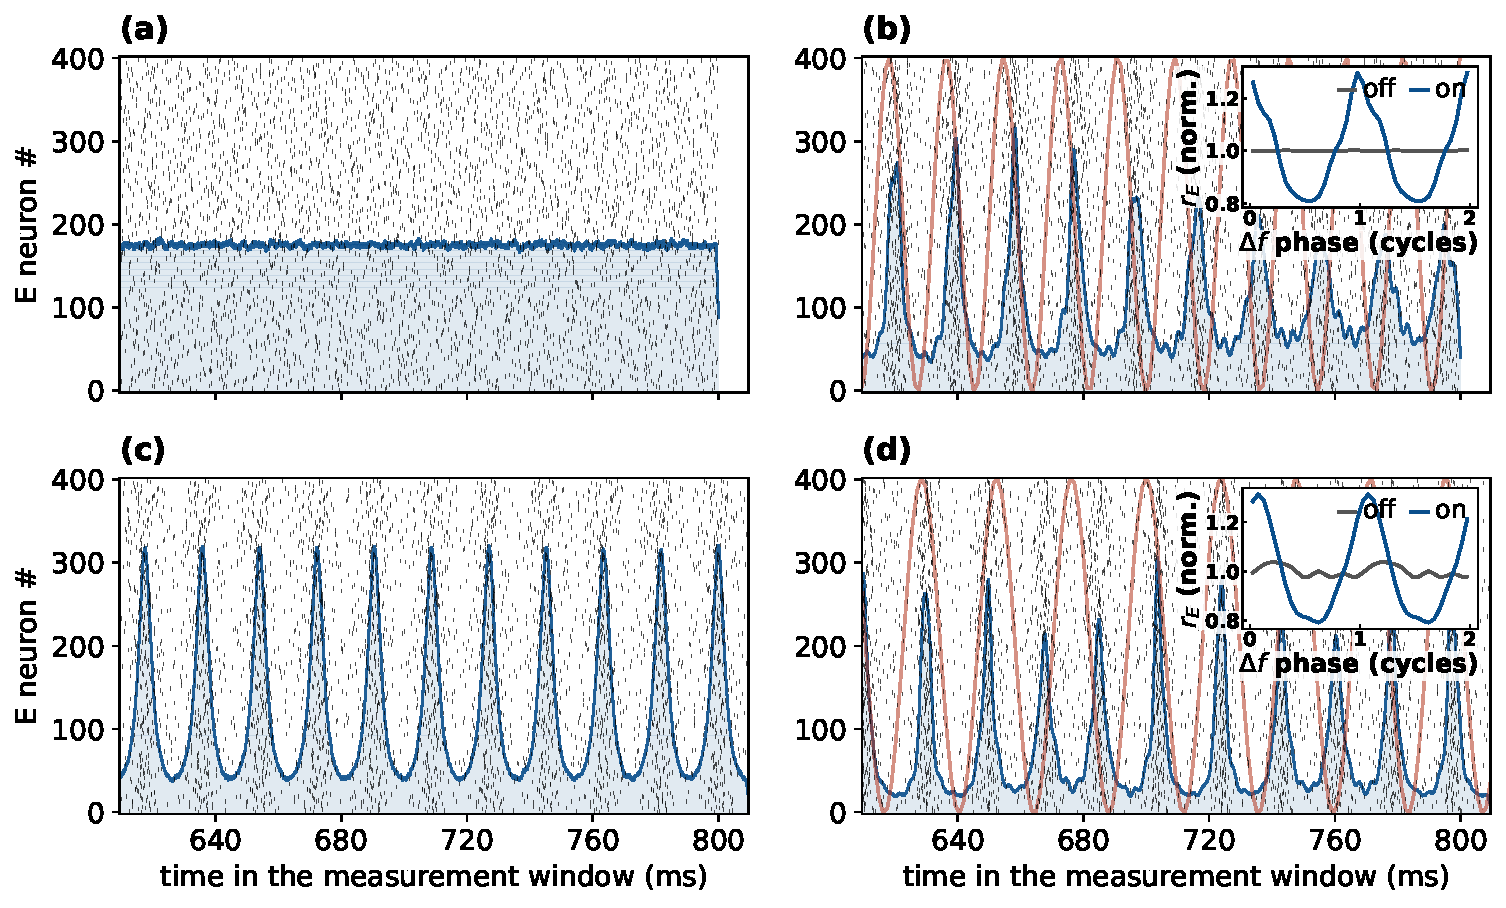
\includegraphics[width=\textwidth]{fig_qif_raster_twotone.pdf}
\caption{\DIFdelbeginFL \DIFdelFL{\textbf{Beat-locked and gamma activity coexist in the QIF network.} }\DIFdelendFL \DIFaddbeginFL \DIFaddFL{\textbf{Beat-locked activity superposed on gamma.}
QIF network, }\DIFaddendFL $N=8000$ \DIFdelbeginFL \DIFdelFL{excitatory and inhibitory quadratic integrate-and-fire neurons whose exact mean field is the
NMM2 PING circuit (Eq.~\eqref{eq:nmm2-ping}). These are finite-amplitude examples
(}\DIFdelendFL \DIFaddbeginFL \DIFaddFL{per population, }\DIFaddendFL $A_f=35$ per tone, carrier \DIFdelbeginFL \DIFdelFL{$f_c=300$}\DIFdelendFL \DIFaddbeginFL \DIFaddFL{$300$}\DIFaddendFL ~Hz\DIFdelbeginFL \DIFdelFL{)}\DIFdelendFL .
Black ticks\DIFdelbeginFL \DIFdelFL{are $E$ spikes (}\DIFdelendFL \DIFaddbeginFL \DIFaddFL{: }\DIFaddendFL 400 \DIFdelbeginFL \DIFdelFL{of 8000),
}\DIFdelendFL \DIFaddbeginFL \DIFaddFL{E neurons; }\DIFaddendFL blue\DIFdelbeginFL \DIFdelFL{is the }\DIFdelendFL \DIFaddbeginFL \DIFaddFL{: }\DIFaddendFL smoothed \DIFdelbeginFL \DIFdelFL{population }\DIFdelendFL rate on \DIFdelbeginFL \DIFdelFL{a separate }\DIFdelendFL \DIFaddbeginFL \DIFaddFL{its own }\DIFaddendFL scale\DIFdelbeginFL \DIFdelFL{, and }\DIFdelendFL \DIFaddbeginFL \DIFaddFL{; }\DIFaddendFL red\DIFdelbeginFL \DIFdelFL{is the TI }\DIFdelendFL \DIFaddbeginFL \DIFaddFL{:
}\DIFaddendFL envelope in arbitrary units. \DIFaddbeginFL \DIFaddFL{The last $200$~ms are shown.
}\DIFaddendFL \emph{(a,b)} \DIFdelbeginFL \DIFdelFL{Field-free stable state ($\bar\eta=0.85$), TI }\DIFdelendFL \DIFaddbeginFL \DIFaddFL{Field }\DIFaddendFL off\DIFdelbeginFL \DIFdelFL{then }\DIFdelendFL \DIFaddbeginFL \DIFaddFL{/}\DIFaddendFL on at \DIFdelbeginFL \DIFdelFL{$\Delta f=55$}\DIFdelendFL \DIFaddbeginFL \DIFaddFL{$\bar\eta=0.85$, beat $55$}\DIFaddendFL ~Hz\DIFdelbeginFL \DIFdelFL{. The field-on response is dominated by field-induced }\DIFdelendFL \DIFaddbeginFL \DIFaddFL{: induced }\DIFaddendFL gamma
near $52$~Hz \DIFdelbeginFL \DIFdelFL{(depth $0.70$), with a smaller beat component (depth $0.29$)}\DIFdelendFL \DIFaddbeginFL \DIFaddFL{dominates}\DIFaddendFL . \emph{(c,d)} \DIFdelbeginFL \DIFdelFL{Field-free oscillatory state ($\bar\eta=1.5$), TI }\DIFdelendFL \DIFaddbeginFL \DIFaddFL{Field }\DIFaddendFL off\DIFdelbeginFL \DIFdelFL{then }\DIFdelendFL \DIFaddbeginFL \DIFaddFL{/}\DIFaddendFL on at \DIFdelbeginFL \DIFdelFL{$\Delta f=42$~Hz. Gamma near $53$--$54$~Hz dominates the raster}\DIFdelendFL \DIFaddbeginFL \DIFaddFL{$\bar\eta=1.5$}\DIFaddendFL ,
\DIFdelbeginFL \DIFdelFL{with depth about
four times the }\DIFdelendFL beat \DIFdelbeginFL \DIFdelFL{component's $0.23$; their coexistence gives slow variations in
burst height. Depth is line amplitude divided by mean rate. The final $200$}\DIFdelendFL \DIFaddbeginFL \DIFaddFL{$42$}\DIFaddendFL ~\DIFdelbeginFL \DIFdelFL{ms of the
common measurement interval are shown}\DIFdelendFL \DIFaddbeginFL \DIFaddFL{Hz: autonomous gamma remains dominant}\DIFaddendFL .
\DIFdelbeginFL \DIFdelFL{\emph{Insets} in \emph{(b,d)} }\DIFdelendFL \DIFaddbeginFL \DIFaddFL{Insets }\DIFaddendFL fold \DIFdelbeginFL \DIFdelFL{the
}\DIFdelendFL rate on beat phase over $44$ and $34$ cycles\DIFdelbeginFL \DIFdelFL{(off gray}\DIFdelendFL , \DIFdelbeginFL \DIFdelFL{on blue)}\DIFdelendFL \DIFaddbeginFL \DIFaddFL{respectively}\DIFaddendFL ,
normalized to each condition's mean \DIFaddbeginFL \DIFaddFL{(off gray, on blue; scale 0--2)}\DIFaddendFL .
\DIFdelbeginFL \DIFdelFL{This averaging }\DIFdelendFL \DIFaddbeginFL \DIFaddFL{Folding }\DIFaddendFL suppresses non-beat-locked gamma and \DIFdelbeginFL \DIFdelFL{displays }\DIFdelendFL \DIFaddbeginFL \DIFaddFL{exposes }\DIFaddendFL the smaller beat component\DIFdelbeginFL \DIFdelFL{on a common $0$--$2$ scale. The fold alone }\DIFdelendFL \DIFaddbeginFL \DIFaddFL{;
it }\DIFaddendFL does not establish gamma-amplitude gating or phase capture.}
\label{fig:qif_raster}
\end{figure}

\begin{figure}[t!]
\centering
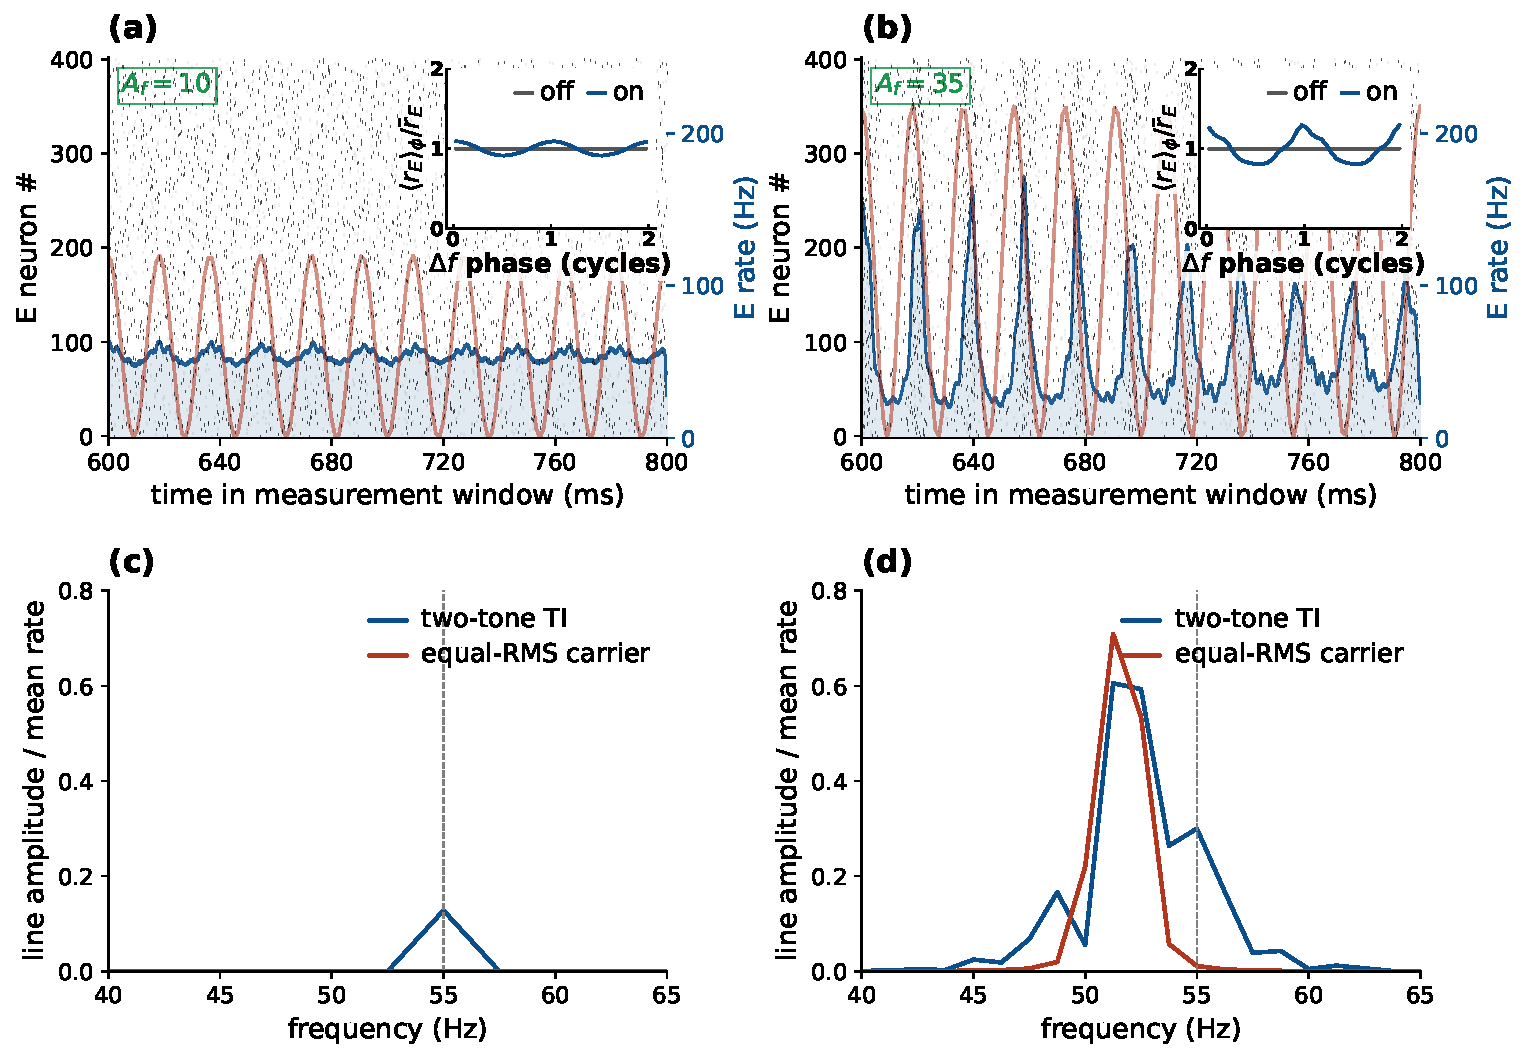
\includegraphics[width=\textwidth]{fig_qif_regimes.pdf}
\caption{\DIFdelbeginFL \DIFdelFL{\textbf{Beat modulation below and across the induced-gamma transition.}
All panels use }\DIFdelendFL \DIFaddbeginFL \DIFaddFL{\textbf{TI and an equal-power carrier across the gamma threshold.}
Background }\DIFaddendFL $\bar\eta=0.85$, carrier $300$~Hz, \DIFdelbeginFL \DIFdelFL{and TI }\DIFdelendFL beat $55$~Hz.
\emph{(a,b)} \DIFdelbeginFL \DIFdelFL{Spiking-network responses }\DIFdelendFL \DIFaddbeginFL \DIFaddFL{Spiking network }\DIFaddendFL at $A_f=10$ and $35$ per tone\DIFdelbeginFL \DIFdelFL{, respectively}\DIFdelendFL \DIFaddbeginFL \DIFaddFL{.
Black}\DIFaddendFL : \DIFdelbeginFL \DIFdelFL{black ticks are spikes from }\DIFdelendFL 400 of 8000 E neurons; blue\DIFdelbeginFL \DIFdelFL{is the smoothed }\DIFdelendFL \DIFaddbeginFL \DIFaddFL{: }\DIFaddendFL population rate on \DIFdelbeginFL \DIFdelFL{the }\DIFdelendFL \DIFaddbeginFL \DIFaddFL{a }\DIFaddendFL common \DIFdelbeginFL \DIFdelFL{right-axis }\DIFdelendFL scale\DIFdelbeginFL \DIFdelFL{, and }\DIFdelendFL \DIFaddbeginFL \DIFaddFL{;
}\DIFaddendFL red\DIFdelbeginFL \DIFdelFL{is the }\DIFdelendFL \DIFaddbeginFL \DIFaddFL{: }\DIFaddendFL envelope\DIFdelbeginFL \DIFdelFL{in arbitrary units}\DIFdelendFL . Insets show \DIFdelbeginFL \DIFdelFL{phase-folded rate divided by its mean }\DIFdelendFL \DIFaddbeginFL \DIFaddFL{mean-normalized phase folds }\DIFaddendFL (off gray, on blue)\DIFdelbeginFL \DIFdelFL{, on the
same scale}\DIFdelendFL .
\DIFdelbeginFL \DIFdelFL{The beat }\DIFdelendFL \DIFaddbeginFL \DIFaddFL{Beat }\DIFaddendFL depths are $0.093$ and $0.290$, \DIFdelbeginFL \DIFdelFL{and the }\DIFdelendFL \DIFaddbeginFL \DIFaddFL{with }\DIFaddendFL mean-rate increases \DIFdelbeginFL \DIFdelFL{are }\DIFdelendFL \DIFaddbeginFL \DIFaddFL{of }\DIFaddendFL $2.8\%$
and $10.5\%$\DIFdelbeginFL \DIFdelFL{. At }\DIFdelendFL \DIFaddbeginFL \DIFaddFL{; }\DIFaddendFL the larger \DIFdelbeginFL \DIFdelFL{amplitude, non-beat-locked }\DIFdelendFL \DIFaddbeginFL \DIFaddFL{input also induces }\DIFaddendFL gamma\DIFdelbeginFL \DIFdelFL{dominates
the raster and is suppressed by the fold}\DIFdelendFL .
\emph{(c,d)} \DIFdelbeginFL \DIFdelFL{Corresponding mean-field }\DIFdelendFL \DIFaddbeginFL \DIFaddFL{Mean-field }\DIFaddendFL spectra under TI (blue) and \DIFdelbeginFL \DIFdelFL{an equal-RMS
single }\DIFdelendFL \DIFaddbeginFL \DIFaddFL{one }\DIFaddendFL carrier \DIFaddbeginFL \DIFaddFL{of peak
amplitude $\sqrt2 A_f$ }\DIFaddendFL (red), \DIFdelbeginFL \DIFdelFL{whose peak amplitude is $\sqrt{2}A_f$. Line amplitude is
}\DIFdelendFL normalized \DIFdelbeginFL \DIFdelFL{by each trace's }\DIFdelendFL \DIFaddbeginFL \DIFaddFL{to }\DIFaddendFL mean \DIFaddbeginFL \DIFaddFL{rate. Both induce gamma
at the larger input}\DIFaddendFL ; \DIFaddbeginFL \DIFaddFL{TI adds }\DIFaddendFL the \DIFdelbeginFL \DIFdelFL{dashed line marks }\DIFdelendFL $55$~Hz \DIFaddbeginFL \DIFaddFL{beat (dashed)}\DIFaddendFL .
\DIFdelbeginFL \DIFdelFL{Spectra use a
}\DIFdelendFL Hann \DIFdelbeginFL \DIFdelFL{window over }\DIFdelendFL \DIFaddbeginFL \DIFaddFL{windows span }\DIFaddendFL $800$~ms after $800$~ms settling.
\DIFdelbeginFL \DIFdelFL{Both waveforms induce gamma
at the larger amplitude, while TI produces the additional beat response.
Increasing the measurement window from $0.8$ to $3.2$~s reduces
the carrier's apparent $55$~Hz depth from $0.011$ to $9.2\times10^{-5}$,
consistent with spectral leakage, while TI's beat depth remains $0.30$--$0.31$. The carrier comparison is a mean-field result. The spiking
}\DIFdelendFL \DIFaddbeginFL \DIFaddFL{Spiking }\DIFaddendFL panels \DIFdelbeginFL \DIFdelFL{retain }\DIFdelendFL \DIFaddbeginFL \DIFaddFL{use }\DIFaddendFL $V_{\rm peak}=100$; \DIFdelbeginFL \DIFdelFL{at cutoffs $200$--$400$, the $A_f=10$
}\DIFdelendFL \DIFaddbeginFL \DIFaddFL{weak-drive }\DIFaddendFL depth \DIFdelbeginFL \DIFdelFL{ranges from $0.121$ to $0.141$ across the two tested steps
(\S\ref{sec:qif-methods})}\DIFdelendFL \DIFaddbeginFL \DIFaddFL{remains cutoff-sensitive}\DIFaddendFL .}
\label{fig:qif_regimes}
\end{figure}

At $\bar\eta=1.5$, gamma activity is already present without stimulation. With the
field on, the rhythm near $53$--$54$~Hz remains about four times larger than the
$42$~Hz beat-locked component. Gamma therefore dominates the raster in panel~(d);
the coexistence of the rhythms produces slower variations in burst height. Folding the
rate on the beat phase suppresses the non-beat-locked gamma and exposes the smaller
component. The inset shows that phase average, not the full rate variation.

\DIFaddbegin \DIFadd{Mixing of slow and fast inputs can generate endogenous amplitude modulation
\cite{ruffini2025ham}; here the recovered beat mixes with the ongoing gamma.
}\DIFaddend The spectrum has sidebands near $95$ and $11$~Hz
(Fig.~\ref{fig:qif_timing}b), establishing nonlinear mixing without distinguishing
gamma-amplitude gating from phase modulation; field-free gamma frequencies agree
between the spiking network and mean field (panel~a).

At $A_f=35$, the mean rate rises by about $8$--$11\%$ across the two conditions, while the beat modulation
depth, $A_\Omega/\langle r_E\rangle$, rises from below $0.003$ to $0.29$
($\bar\eta=0.85$) and $0.23$ ($\bar\eta=1.5$) (Fig.~\ref{fig:qif_timing}c). Modulation is about three times the relative mean-rate change, but per-neuron
locking is weak: the pairwise phase consistency of single-neuron spike phases at
$\Delta f$ rises from its field-free control (median $-0.02$) to a median of
$0.003$--$0.005$, and the pooled vector strength from below $0.02$ to $0.12$--$0.13$. The
population's beat-locked component is built from many weakly biased cells; these
finite-amplitude runs do not establish its size under weak physiological stimulation.

\section{Discussion}\label{sec:discussion}
\DIFdelbegin \DIFdel{Access sets the local polarization, detection generates the beat, and the circuit
sets its amplification. }\DIFdelend \DIFaddbegin \subsection{\DIFadd{Cellular access and mixing require separate calibration}}
\DIFaddend Esmaeilpour et al.\
\cite{esmaeilpour2021} already related network TI sensitivity to short, axon-like
membrane times and distinguished sensitivity from selectivity mediated by
network adaptation. Here the exact QIF mean field connects static and dynamic
mixing, the weak-input product law determines spatial weighting, and matching
the generated drive exposes the linear amplifier shared by TI and tACS.

At \DIFdelbegin \DIFdel{extracellular }\DIFdelend fields of order $1$~V/m, \DIFdelbegin \DIFdel{voltage-gated }\DIFdelend channels respond through membrane polarization\DIFdelbegin \DIFdel{: the }\DIFdelend \DIFaddbegin \DIFadd{,
well below the fields associated with }\DIFaddend direct protein effects
\DIFdelbegin \DIFdel{reviewed by Cifra et al.\
\cite{cifra2026}occur at $10$~kV/m to GV/m, with protocol- and molecule-dependent
thresholds; that review excludes fields below $0.1$~kV/m, where it expects direct
effects to be negligible against thermal noise.}\DIFdelend \DIFaddbegin \DIFadd{\cite{cifra2026}.}\footnote{\DIFadd{The review describes direct effects at $10$~kV/m
to GV/m, depending on molecule and protocol. It excludes fields below
$0.1$~kV/m, where it expects direct effects to be negligible against thermal noise.}} \DIFaddend Presynaptic terminals can polarize
more strongly than somata \cite{rahman2013,aberra2023,chakraborty2018}, but small
size alone does not imply fast charging: specific membrane resistance times
capacitance is area-independent, while conductance, geometry, and stimulation
mode determine the response.

\DIFaddbegin \DIFadd{The short-time cases in }\DIFaddend Table~\ref{tab:doors} \DIFdelbegin \DIFdel{summarizes the measurements and models that motivate shorter
access times; their transfer under TI remains to be calibrated. }\DIFdelend \DIFaddbegin \DIFadd{motivate a preparation-dependent
access hypothesis. Reducing QIF membrane time by $10$--$100$-fold tests that
hypothesis; it does not calibrate TI access. Related model settings and strong-pulse
measurements are compared in the supplement (\S\ref{supp:access}).
}\ifjne\else
\subsection{\DIFadd{Access assumptions in related models}}
\DIFadd{Short access times motivate the model but remain preparation-dependent.
}\DIFaddend The $1$ and $0.4$~ms \DIFdelbegin \DIFdel{network sensitivity }\DIFdelend cases of \cite{esmaeilpour2021} precede \DIFdelbegin \DIFdel{the present }\DIFdelend \DIFaddbegin \DIFadd{our }\DIFaddend effective-time
hypothesis. Luff et al.'s pulse-width-modulated TI \DIFdelbegin \DIFdel{(PWM-TI) model uses a }\DIFdelend \DIFaddbegin \DIFadd{model uses }\DIFaddend $1$~ms \DIFdelbegin \DIFdel{passive response }\DIFdelend within a
$1$--$100$~ms \DIFdelbegin \DIFdel{parameter }\DIFdelend \DIFaddbegin \DIFadd{passive-time }\DIFaddend sweep \cite{luff2024}. \DIFdelbegin \DIFdel{Separately, }\DIFdelend \DIFaddbegin \DIFadd{The $0.7~\mu$s charging
measured by }\DIFaddend Semenov et al.\ \DIFdelbegin \DIFdel{\cite{semenov2025} measured field-induced membrane charging near $0.7~\mu$s in
isolated neurons under strong , }\DIFdelend \DIFaddbegin \DIFadd{under strong }\DIFaddend microsecond field pulses
\DIFdelbegin \DIFdel{. This is }\DIFdelend \DIFaddbegin \DIFadd{\cite{semenov2025} concerns }\DIFaddend a different response mode from intracellular
current charging or periaxonal conduction. \DIFdelbegin \DIFdel{Access time and field coupling remain preparation-dependent. }\DIFdelend A $10$--$100$-fold reduction in
\DIFdelbegin \DIFdel{a }\DIFdelend QIF membrane time is therefore a sensitivity hypothesis\DIFdelbegin \DIFdel{. Its
population-level consequence can be studied through the existing }\DIFdelend \DIFaddbegin \DIFadd{, whose population
consequence follows from the }\DIFaddend slow-synapse limit\DIFdelbegin \DIFdel{, with each physical filter included once; a new periaxonal circuit is not
needed for that limiting argument}\DIFdelend .

\DIFdelbegin \DIFdel{At weak input, smooth cellular contributions with a nonzero second-order term
combine into a quadratic mixing }\DIFdelend \DIFaddbegin \fi

\DIFadd{The quadratic law specifies the leading mixing operation, not its }\DIFaddend coefficient.
QIF derives one realization\DIFdelbegin \DIFdel{without
requiring identification of each channel. It connects cellular mixing \cite{mirzakhalili2020,luff2024mixer} with the network dependence }\DIFdelend \DIFaddbegin \DIFadd{; cellular mixing measured or modeled in single
neurons \cite{mirzakhalili2020,luff2024mixer} can feed the recurrent
amplification }\DIFaddend seen in slices and simulations \cite{caldas2024,karimi2024}.
\DIFdelbegin \DIFdel{Cellular mixing and
circuit amplification are therefore not competing explanations. }%DIFDELCMD <

%DIFDELCMD < %%%
\DIFdel{Weak amplitude alone does not make that coefficient static . Fast population relaxation relative to synapses gives the NMM2 slow-synapse limit; relaxation
must also be }\DIFdelend \DIFaddbegin \DIFadd{These are complementary stages. A static curve describes mixing only when
population relaxation is }\DIFaddend fast relative to the carrier \DIFdelbegin \DIFdel{for curvature to describe its mixing.
Outside that limit the coefficient is dynamic. Its magnitude, phase, and
frequency dependenceremain model-specific, while the static }\DIFdelend \DIFaddbegin \DIFadd{as well as the synapses.
Otherwise the coefficient retains its own frequency dependence, while }\DIFaddend slope
converts slow input into rate and enters recurrent gain\DIFdelbegin \DIFdel{(\S\ref{sec:nmm})}\DIFdelend .

\DIFaddbegin \subsection{\DIFadd{Detector laws predict different spatial responses}}
\DIFaddend A spatial TI dose map depends on this physiology. The usual envelope-modulation
map assumes a response determined by envelope excursion; the square-law map
instead weights it by the larger local polarization (Eq.~\eqref{eq:reweight}).
\DIFdelbegin \DIFdel{Its accompanying DC }\DIFdelend \DIFaddbegin \DIFadd{The accompanying steady }\DIFaddend source follows the summed carrier intensities\DIFdelbegin \DIFdel{under the
conditions of \S\ref{sec:dc},
providing an operating-point shift that
the equal-RMS carrier control isolates and that can cross the population Hopf
(\S\ref{sec:qif}).
Both idealized mean
maps obey the boundary-maximum restriction of
\S\ref{sec:dc}; the beat map does not}\DIFdelend \DIFaddbegin \DIFadd{,
weighted by the local detector coefficient. Under uniform conductivity,
access, and detection, its largest magnitude and the ideal envelope mean
lie on compartment boundaries. The beat can instead peak inside}\DIFaddend .
Orientation, access, operating point, and network susceptibility further shape
the response. A sharp rectifier can approximate
envelope following over a finite amplitude range; smoothing or heterogeneity
can restore quadratic behavior at smaller inputs. The amplitude and harmonic
tests in \S\ref{sec:transduction-methods} distinguish these regimes.

Violante et al.\ \cite{violante2023} demonstrated envelope steering and a
change in hippocampal physiology using different measurements. Their field
models and cadaver recordings supported anterior envelope steering when the
current ratio changed from $2+2$~mA (1:1) to $1+3$~mA (1:3) through the same
electrode pairs. In participants, stimulation was confined to the 32~s
encoding stage of each block. The 1:3 condition reduced the encoding-evoked
blood-oxygen-level-dependent (BOLD) response relative to sham ($P=0.006$) and
1:1 ($P=0.015$); 1:1 did not differ significantly from sham ($P=0.953$).
The reduction was nominally largest anteriorly, but the stimulation-by-region
interaction was not significant ($P=0.76$). The voxelwise sham--1:3 comparison
found significant reductions in 30\% of anterior, 25\% of posterior, and 2\% of
middle hippocampal voxels. Significant BOLD reductions thus extended beyond
the anterior envelope focus.

All three geometric maps change between these current conditions, so a condition
difference alone cannot identify the detector. In \DIFdelbegin \DIFdel{our }\DIFdelend IXI002 \DIFdelbegin \DIFdel{calculation
(\S\ref{sec:fem-results}, Fig.~\ref{fig:fem}), the envelope focus moves 2.5~mm
anteriorly, whereas the quadratic beat retains its pattern }\DIFdelend \DIFaddbegin \DIFadd{the quadratic beat pattern remains fixed }\DIFaddend and falls to $3/4$ of
its value everywhere\DIFdelbegin \DIFdel{at fixed neural state. }\DIFdelend \DIFaddbegin \DIFadd{. Mean-square polarization instead changes its pattern and
rises where the posterior pair contributes sufficiently strongly (supplement,
\S\ref{supp:steering-algebra}). Equal summed currents do not match local RMS
polarization.
}\ifjne\else
\subsection{\DIFadd{Mean-square change under current-ratio steering}}\label{supp:steering-algebra}
\DIFaddend The mean-square polarization
changes by $\mathcal I_{1:3}/\mathcal I_{1:1}
=(\mathcal P_1^2+9\mathcal P_2^2)/[4(\mathcal P_1^2+\mathcal P_2^2)]$,
exceeding one only where $|\mathcal P_2|>\sqrt{3/5}|\mathcal P_1|
\approx0.775|\mathcal P_1|$. Its hippocampal mean rises by 24\% and its focus
moves 4.5~mm posteriorly. Equal summed currents therefore do not match local
RMS polarization.

\DIFdelbegin \DIFdel{The mean-square map also predicts a physiological effect: at second order it
sets the steady rate source $Y_{\rm DC}=\tfrac12\Sig''(v^*)\mathcal I$
(\S\ref{sec:dc}). With }\DIFdelend \DIFaddbegin \fi

\DIFadd{At }\DIFaddend spatially uniform, fixed curvature, \DIFdelbegin \DIFdel{its }\DIFdelend \DIFaddbegin \DIFadd{the }\DIFaddend 24\% increase in hippocampal
\DIFdelbegin \DIFdel{mean }\DIFdelend \DIFaddbegin \DIFadd{mean-square polarization }\DIFaddend predicts a 24\% \DIFdelbegin \DIFdel{larger mean-rate source in magnitude,
with the
sign set by the curvature. Recurrence then }\DIFdelend \DIFaddbegin \DIFadd{increase in the magnitude of the
steady rate source $Y_{\rm DC}=\Sig''(v^*)\mathcal I/2$. Curvature sets
its sign; recurrence }\DIFaddend determines the final rate response. By comparison, the hippocampal mean envelope excursion falls by
45\%, and both the projected and isotropic quadratic beat maps fall by 25\%.
A response linear in the quadratic beat thus decreases; its own rectified
mean shift scales as $(3/4)^2\approx0.56$ at fixed state in the weak-response
limit (\S\ref{sec:timing}). Of these hippocampal map averages, only the
mean-square polarization increases under 1:3, consistent with a larger
magnitude of BOLD reduction if the steady source lowers activity and the
hemodynamic response preserves that ordering. A slow, approximately linear
hemodynamic readout suppresses the zero-mean $5$~Hz beat at first order while
retaining a slow shift over the stimulation window. Such a shift can add to
the encoding-evoked response or alter its operating point; nonlinear neural
or vascular responses can also convert the beat into a mean change.

\DIFdelbegin \DIFdel{This interpretation remains conditional:
}\DIFdelend \DIFaddbegin \DIFadd{Locally, }\DIFaddend the envelope excursion rises where $|\mathcal P_1|>2|\mathcal P_2|$,
reaching $1.5\times$ where $|\mathcal P_1|\geq3|\mathcal P_2|$,
allowing a spatially selective or
thresholded envelope response, and the nonsignificant 1:1--sham difference
does not establish a null effect. \DIFdelbegin \DIFdel{Neither hippocampal curvature nor the
}\DIFdelend \DIFaddbegin \DIFadd{Hippocampal curvature and }\DIFaddend recurrent and hemodynamic gains are \DIFdelbegin \DIFdel{calibrated here;
spatially varying
curvature can also }\DIFdelend \DIFaddbegin \DIFadd{uncalibrated;
heterogeneous curvature can }\DIFaddend change the mean-source ratio. \DIFdelbegin \DIFdel{Neither the BOLD contrast
nor the reported functional-connectivity changes directly measure the beat
or the steady source . The voxelwise pattern therefore cannot be matched to
one of these maps without }\DIFdelend \DIFaddbegin \DIFadd{BOLD and functional
connectivity measure neither source directly, so interpreting their spatial
pattern requires }\DIFaddend a neural and hemodynamic readout model. A spatially resolved beat measurement at controlled state would
test envelope steering against the fixed quadratic pattern; an equal-power
unmodulated-carrier control would isolate effects of the steady source under
the second-order matching conditions of \S\ref{sec:dc}.

\DIFaddbegin \subsection{\DIFadd{Field-induced oscillations and resonant amplification}}
\DIFaddend At higher intensities, TI and unmodulated kHz fields can have similar excitation
thresholds, with modulation patterning firing rather than lowering the threshold
\cite{opancar2025,semenov2025}; some peripheral responses do not require envelope
extraction \cite{peripheral2023}. The weak-input calculation instead describes
modulation of ongoing activity \cite{vieira2024,missey2026}, excluding direct
carrier-evoked spiking and conduction block. The finite-amplitude QIF examples
show a related circuit transition: the mean shift crosses the Hopf, inducing
gamma alongside the beat response. Its boundary depends on both field amplitude
and the initial distance from the bifurcation. These examples and the laminar
extension go beyond the weak-input expansion without establishing physiological
thresholds.

The \DIFdelbegin \DIFdel{recurrent amplifier is }\DIFdelend \DIFaddbegin \DIFadd{pinned JR comparison (\S\ref{sec:tacs-results}) isolates the recurrent
susceptibility }\DIFaddend shared with direct low-frequency stimulation\DIFdelbegin \DIFdel{. Our
coupling sweep fixes the JR field-free operating point and its local curvature
while changing recurrent gain. A direct in-band drive shows the same
$1/\gamma$ growth and resonance sharpening (Fig.~\ref{fig:tacs})}\DIFdelend , consistent with
\DIFdelbegin \DIFdel{the known resonant susceptibility of recurrent }\DIFdelend \DIFaddbegin \DIFadd{previous }\DIFaddend excitatory--inhibitory \DIFdelbegin \DIFdel{networks
\cite{ledoux2011,clusella2023}.
Near the Hopf, this is temporal critical slowing in a mean-field model, not evidence of }\DIFdelend \DIFaddbegin \DIFadd{network models \cite{ledoux2011,clusella2023}.
Near-Hopf temporal slowing does not establish }\DIFaddend a diverging spatial correlation
length. Related models \DIFdelbegin \DIFdel{already }\DIFdelend reproduce tACS entrainment and AM-driven phase locking
\cite{ali2013,negahbani2018,krause2023}. \DIFdelbegin \DIFdel{When TI and tACS are matched
for effective in-band input, observable, and operating state
, they share }\DIFdelend \DIFaddbegin \DIFadd{Matching generated input, readout, and state
makes }\DIFaddend the linear amplifier \DIFdelbegin \DIFdel{. Within linear response, resonance alone therefore gives TI no efficiency advantage. At finite amplitudethe response ratio can change near
the Hopf, as the coupling sweep demonstrates (\S\ref{sec:tacs-results}); its value then
depends on drive amplitude and the driven state as well as on field-free damping. }\DIFdelend \DIFaddbegin \DIFadd{common to TI and tACS; at finite amplitude, their
response ratio also depends on stimulation-induced state shifts.
}\DIFaddend

\DIFaddbegin \DIFadd{A reverberation time $\tau_{\rm rev}=1/\gamma$ gives a near-Hopf
quality factor $\mathcal Q=\pi f_0\tau_{\rm rev}$ and power bandwidth
approximately $1/(\pi\tau_{\rm rev})$. Population relaxation over a few hundred
milliseconds \cite{wilting2018} would give a quality factor of order ten at
$10$~Hz and a bandwidth of order $1$~Hz. This is an order-of-magnitude comparison:
the measured relaxation is not specific to the alpha mode. Narrow amplification
also makes detuning consequential.
}

\subsection{\DIFadd{Efficiency depends on the generated drive}}
\DIFaddend Absolute response estimates \DIFdelbegin \DIFdel{remain sensitive to }\DIFdelend \DIFaddbegin \DIFadd{depend on }\DIFaddend access and transduction.
Measured DC field-to-voltage couplings are $0.12$--$0.18$~mV per V/m in
hippocampus ($0.21$ at $10$~Hz AC) \cite{bikson2004,deans2007} and reach about
$0.5$~mV per V/m in cortical
L5/6 pyramidal cells \cite{radman2009}; human cortical fields near $0.8$~V/m have
been reported at $2$~mA \cite{huang2017,huang2017corr}. These static couplings do
not fix the coupling at kHz. \DIFdelbegin \DIFdel{For equal TI carrier polarizations$\varepsilon$}\DIFdelend \DIFaddbegin \DIFadd{At equal per-carrier and direct-input polarizations}\DIFaddend ,
the JR \DIFdelbegin \DIFdel{beat drive is $\Sig''\varepsilon^2/2$, whereas a direct drive of the same
peak polarization gives $2\Sig'\varepsilon$. Their leading amplitude ratio is
$\mathcal R_{\rm det}\simeq|\Sig''|\varepsilon/(4\Sig')$: the relative efficiency decreases
as the input is weakened in this perturbative regime. A larger recurrent gain
amplifies both drives.
}%DIFDELCMD <

%DIFDELCMD < %%%
\DIFdel{For scale, a reverberation time $\tau_{\rm rev}=1/\gamma$ gives a near-Hopf
quality factor $\mathcal Q=\pi f_0\tau_{\rm rev}$ and power bandwidth
approximately $1/(\pi\tau_{\rm rev})$. Population relaxation over a few hundred
milliseconds \cite{wilting2018} would give a quality factor of order ten at
$10$~Hz and a bandwidth of order $1$~Hz. This is an order-of-magnitude comparison:
the measured relaxation is not specific to the alpha mode. Narrow amplification
also makes detuning consequential.
}%DIFDELCMD <

%DIFDELCMD < %%%
\DIFdel{Primate measurements illustrate the limits of an efficiency comparison.
Vieira et al.\ \cite{vieira2024} reported two distinct experiments. Their
two-pair TI comparison gave a phase-locking effect ratio of $0.34$ against
tACS (95\% confidence interval $0.04$}\DIFdelend \DIFaddbegin \DIFadd{steady and beat sources are approximately $2$}\DIFaddend --\DIFdelbegin \DIFdel{$0.65$, 65 of 154 neurons), without
correcting for TI currents up to $\pm2.5$~mA per pair versus $\pm1$~mA for tACS.
A separate single-pair AM-tACS control compensated for frequency-dependent
shunting to match extracellular modulation depth. Of twenty cells, ten responded
to either modality and seven to both; in the latter group, median phase-locking
value (PLV)was $0.10$ for AM-tACS and $0.20$ for tACS, against $0.043$ at baseline. The reported TI modulation depths were about $0.5$}\DIFdelend \DIFaddbegin \DIFadd{$5\%$ of the corresponding
tDCS and tACS sources for $0.1$}\DIFaddend --\DIFdelbegin \DIFdel{$0.62$~V/m.
These weaker
TI and AM effects are compatible with a weaker generated beat drive, but neither
experiment matched polarization at the mixer, and PLV depends on baseline and
state. They therefore do not calibrate this paper's detector coefficient; that
requires the same timing readout across a local-polarization amplitude sweep. }\DIFdelend \DIFaddbegin \DIFadd{$0.3$~mV at the pinned operating point
(\S\ref{sec:dc}). The following estimate instead matches the total TI peak.
With direct amplitude $2\varepsilon$, the leading ratio is
$\mathcal R_{\rm det}\simeq|\Sig''|\varepsilon/(4\Sig')$, half the equal-per-carrier
ratio derived in \S\ref{sec:direct-comparison}. The common recurrent gain cancels.
}\DIFaddend

For an illustrative fast-access budget, take a per-tone field $E_j=0.5$~V/m,
$\lambda_0=0.5$~mV per V/m, $f_c=2$~kHz, and the assumed $\tau_m=0.2$~ms.
Then $\varepsilon=\lambda_0E_j|H_m|\approx0.092$~mV, rounded to $0.1$~mV for
scale; this is an assumed coupling budget, not an inferred polarization in
the recorded cells. At $v^*=8.30$~mV the JR detector gives
$\mathcal R_{\rm det}\approx0.8\%$ for $0.1$~mV, for the generated drive relative to a matched-peak direct input.
The smooth JR detector \DIFdelbegin \DIFdel{is therefore weak under this access budget, even though
recurrence can amplify its output. A measured PLV effect cannot be compared
directly with this drive ratio; }\DIFdelend \DIFaddbegin \DIFadd{generates a small beat under this budget. Recurrence
amplifies both TI and matched direct drives, preserving their linear-response
ratio. Testing the estimate requires }\DIFaddend a polarization-calibrated \DIFdelbegin \DIFdel{amplitude }\DIFdelend sweep with
the same readout\DIFdelbegin \DIFdel{would test the estimate}\DIFdelend \DIFaddbegin \DIFadd{; a measured PLV ratio alone does not supply it}\DIFaddend .

For comparison, the carrier-averaged, matched-peak, open-loop drive ratio has a
numerically estimated supremum of $0.348$ over bounded nondecreasing memoryless
transfers (\DIFdelbegin \DIFdel{App.~\ref{app:bound}}\DIFdelend \DIFaddbegin \DIFadd{supplement, \S\ref{app:bound}, Eq.~\eqref{eq:etasup}}\DIFaddend ). The positive-mixture-of-steps argument extends
the logistic result to this class. Approaching it requires an active transition
sharp relative to the input; for the logistic family at the illustrative
polarizations, this means microvolt widths. The limiting detector is step-like
and has a second-harmonic ratio near $0.15$, distinct from both weak
square-law detection and linear envelope following. This bound does not cover
the dynamic QIF detector or all cellular mechanisms. A larger common matched
polarization does not exceed the class bound; unequal actual polarizations can
instead invalidate the matching. The unequal-current TI ratio and the matched-depth
AM-tACS control do not measure this matched-peak, open-loop ratio.
Thus approaching the ceiling would require leaving the smooth weak-input regime
used here; within that regime, local curvature determines the generated drive.

\DIFdelbegin \DIFdel{Access and mixing require calibration; their values are not fixed by the quadratic law, and cascading }\DIFdelend \DIFaddbegin \DIFadd{The weaker TI effects reported by Vieira et al.\ \cite{vieira2024} are compatible with
a smaller generated beat drive, but their experiments did not match local
polarization at the mixer (supplement, \S\ref{supp:vieira}).
Phase-locking value (PLV) also depends on baseline and state. These comparisons
therefore do not calibrate the detector coefficient; that requires the same
readout across a local-polarization amplitude sweep.
}

\subsection{\DIFadd{Limits of the population description}}
\DIFadd{Cascading }\DIFaddend ordinary synaptic filters cannot \DIFdelbegin \DIFdel{improve accessbecause }\DIFdelend \DIFaddbegin \DIFadd{remedy poor access: }\DIFaddend they attenuate
the carrier before \DIFaddbegin \DIFadd{it reaches }\DIFaddend a subsequent detector\DIFdelbegin \DIFdel{receives it}\DIFdelend .
The response also depends on the neuron model: Hodgkin--Huxley and
Frankenhaeuser--Huxley models reproduce stimulus-evoked firing missed by the tested
leaky, exponential, and adaptive-exponential integrate-and-fire models
\cite{plovie2025}, without invalidating the weak-input expansion. Noise,
heterogeneity beyond the assumed excitability distribution, and intercolumn
interactions can broaden or shift the deterministic resonances. Human evidence
is mixed, including peripheral effects without central effects \cite{iszak2023}
and null occipito-parietal alpha-power modulation \cite{mansourinezhad2025}.
Testing this mechanism therefore requires access, generated beat, and network
tuning measured in the same preparation.

\subsection{Falsifiable predictions and tests}\label{sec:predictions}
Table~\ref{tab:predictions} separates tests of access, detection, and amplification
from observations already consistent with the model. Quantitative reanalysis of
the timing and synaptic-blockade data requires the amplitude and harmonic controls
of \S\ref{sec:transduction-methods}, with detector and network changes measured
separately.

\DIFaddbegin \DIFadd{Network filtering must be separated from the harmonic signature. At resonance
with $\mathcal Q=10$, a detector ratio of $20\%$ appears as only $0.7\%$,
which could make an envelope follower look quadratic. Driving off resonance
at $\Delta f\simeq f_0/4$ places both harmonics on the flatter part of the
response, where $|G(2\Omega)/G(\Omega)|\approx1.22$--$1.25$ for
$\mathcal Q=3$--$30$. Alternatively, a weak direct tACS sweep can measure
$G$ independently so its effect can be removed from the harmonic ratio.
}

\DIFaddend \begingroup\small
\renewcommand{\arraystretch}{1.15}
\begin{longtable}{@{}>{\raggedright\arraybackslash}p{0.30\textwidth}
 >{\raggedright\arraybackslash}p{0.27\textwidth}
 >{\raggedright\arraybackslash}p{0.35\textwidth}@{}}
\caption{Predictions, existing evidence, and tests. Published observations provide
qualitative comparisons; their quantitative reanalysis remains to be done.}
\label{tab:predictions}\\
\toprule
\textbf{Prediction (model basis)} & \textbf{Existing evidence} & \textbf{Proposed test} \\
\midrule\endfirsthead
\multicolumn{3}{@{}l}{\textit{Table \thetable\ continued}}\\
\toprule
\textbf{Prediction (model basis)} & \textbf{Existing evidence} & \textbf{Proposed test} \\
\midrule\endhead
\midrule\multicolumn{3}{r@{}}{\textit{Continued on next page}}\\\endfoot
\bottomrule\endlastfoot
\textbf{Carrier dependence.} At fixed local polarization, the leading beat is
carrier-independent in the static limit and fast-carrier QIF asymptote, provided
no other circuit mode is excited. Access restores dependence at fixed applied
field; detector dynamics can add it near the crossover.
& \DIFdelbegin \DIFdel{Carrier-frequency comparisons show changes in network sensitivity\cite{esmaeilpour2021} and subthreshold single-cell mixing\cite{luff2024mixer}, without holding measured local carrier polarizations fixed. Thresholds depend on $f_c$
\cite{opancar2025,peripheral2023}, and }\DIFdelend \DIFaddbegin \DIFadd{Network sensitivity, cellular mixing, and thresholds depend on carrier frequency
\cite{esmaeilpour2021,luff2024mixer,opancar2025,peripheral2023}; }\DIFaddend bare kHz fields
have limited effects on hippocampal oscillations \cite{esmaeilpour2020}.
\DIFaddbegin \DIFadd{Local polarizations were not held fixed.
}\DIFaddend & Measure each local polarization while sweeping $f_c$ at fixed beat and state;
normalize the weak beat by their product. Hold network gain fixed or measure it
independently to separate access from residual detector dependence. Measure any
residual cutoff rather than assigning it to a compartment. \\[4pt]
\textbf{Independent carrier amplitudes.} At fixed detector and network gains,
quadratic modulation excursion follows $2|\varepsilon_1\varepsilon_2|$;
an ideal envelope follower tracks $2\min(|\varepsilon_1|,|\varepsilon_2|)$
(Eq.~\eqref{eq:reweight}, Table~\ref{tab:transduction-maps}).
& The unequal-amplitude spatial example separates these maps; a biological test
with independent local-polarization calibration is not supplied here.
& Hold the weaker polarization fixed and vary the stronger, then swap tones.
Keep both inputs weak, frequencies fixed, and the operating state controlled.
Reconstruct the slow-response excursion after correcting network filtering;
a beat lock-in alone does not measure the envelope's full excursion. \\[4pt]
\textbf{Current-ratio steering.} With fixed electrode pairs, frequencies,
access, and neural state, the quadratic beat map scales with
$I_1^{\rm pair}I_2^{\rm pair}$; its normalized pattern does not move.
An envelope follower can instead shift its maximum.
& \DIFdelbegin \DIFdel{Cassar\`a et al.\ identify the }\DIFdelend \DIFaddbegin \DIFadd{The }\DIFaddend product-law restriction \cite{cassara2025part2} \DIFdelbegin \DIFdel{. The }\DIFdelend \DIFaddbegin \DIFadd{holds in }\DIFaddend IXI002
\DIFdelbegin \DIFdel{comparison }\DIFdelend (\S\ref{sec:fem-results})\DIFdelbegin \DIFdel{confirms
the geometric distinction: envelope and mean-square foci move oppositely; the quadratic beat map only rescales. A }\DIFdelend \DIFaddbegin \DIFadd{; a }\DIFaddend physiological beat-map test remains open.
& Vary the current ratio at fixed electrodes and compare normalized beat maps
and target-to-reference ratios, using a cortex-only reference to test deep-target
selectivity. Keep the projection direction fixed at each site,
including any direction chosen to maximize the envelope at a reference ratio.
Measure the DC shift and repeat at lower amplitude to check state dependence.
 \DIFdelbegin \DIFdel{Changing from $2+2$ to $1+3$~mA multiplies envelope excursion by
$0.5$--$1.5$ depending on the local polarization ratio, and the quadratic beat
by $0.75$ everywhere. The mean-square factor is $1.25$ at equal per-current magnitudes,
tending to $0.25$ or $2.25$ where the first or second carrier dominates,
respectively. This last factor weights the signed DC source; it does not
specify excitation or suppression. }\DIFdelend \\[4pt]
\textbf{State and carrier dependence.} The static sigmoid follows $\Sig''$ and
reverses sign at its inflection (PEIX$=0$). Fast-carrier QIF mixes in voltage and
reads the source through rate and network susceptibility; its DC term follows
$F'$ without the same sign rule (\S\ref{sec:dynamic}).
& Cell-type-specific responses (PV versus pyramidal) are reported
\cite{caldas2024}; the detector coefficient remains model-dependent.
& Vary tonic drive and carrier frequency at fixed beat; measure beat amplitude
and phase. Compare with the predicted coefficient after accounting for network
susceptibility. Amplitude changes alone do not isolate detection. \\[4pt]
\textbf{Transduction class.} At a matched site, weak smooth detection with nonzero
curvature gives $Y_\Omega\propto\varepsilon^2$ and a harmonic ratio vanishing as
$\varepsilon\to0$. An ideal envelope follower gives $Y_\Omega\propto\varepsilon$
and ratio $1/5$; a threshold has onset $2\varepsilon=\delta$ and a variable ratio.
& Untested with local-polarization calibration; existing comparisons match
extracellular field rather than $\varepsilon$.
& Sweep amplitude off resonance, reading both the log--log slope and
$|Y_{2\Omega}/Y_\Omega|$. Near resonance, suppression by approximately
$3\mathcal Q$ requires correction with an independently measured
$G(2\Omega)/G(\Omega)$ (\S\ref{sec:transduction-methods}). \\[4pt]
\textbf{Frequency selectivity.} The beat response peaks at the region's resonant
rhythm and grows as $1/\gamma$ near its Hopf; state changes can alter both the
generated drive and the recurrent gain \cite{ruffini2025cfc}.
& The quantitative gain--bandwidth relation is not tested here in biological data.
& Sweep $\Delta f$ through the intrinsic band across brain states and track the
peak frequency, height, and width. \\[4pt]
\textbf{Timing versus rate.} Beat modulation can exceed the mean shift; their ratio
peaks and then falls as the amplified oscillation rectifies
(\S\ref{sec:timing}--\ref{sec:qif}).
& Qualitatively consistent with TI altering spike timing more than mean rate in
primates \cite{vieira2024}.
& Compare beat lock-in with mean-rate change in commensurate effect measures,
retaining the finite-amplitude qualification. \\[4pt]
\textbf{Network readout.} Population nonlinearity and synaptic recurrence contribute
to the measured response.
& Most pyramidal TI responses vanish under synaptic blockade \cite{caldas2024},
supporting network involvement without excluding cellular mixing.
& Test whether synaptic blockade reduces recurrent amplification while preserving
a cellular detector. \\[4pt]
\textbf{Equal-power carrier control.} At second order, equal local RMS
polarization gives the same steady source when the carriers see the same DC
coefficient. TI also supplies a beat; either waveform can induce an oscillation
if the mean shift crosses a bifurcation.
& Demonstrated in the PING mean field (Fig.~\ref{fig:qif_regimes}c,d).
The corresponding spiking-network and in vivo controls are not provided here.
& Compare two tones with one carrier of matched RMS polarization and duration,
checking the DC coefficient across the carrier interval. Measure mean activity,
intrinsic oscillations, and beat lock-in separately to distinguish the steady
shift from the beat response. \\
\end{longtable}
\endgroup

\section{Conclusion}
\DIFdelbegin \DIFdel{For weak perturbations of ongoing activity, }\DIFdelend \DIFaddbegin \DIFadd{TI requires access, detection, and amplification. For weak inputs with }\DIFaddend a
nonzero second-order \DIFdelbegin \DIFdel{response makes
the TI }\DIFdelend \DIFaddbegin \DIFadd{coefficient, detection generates a }\DIFaddend beat proportional
to the product of the local carrier polarizations \DIFdelbegin \DIFdel{,
rather than the envelope minimum. Its steady source
follows }\DIFdelend \DIFaddbegin \DIFadd{and a steady source
proportional to }\DIFaddend their summed squares\DIFdelbegin \DIFdel{;
the magnitude of this source and the ideal envelope mean have no strict interior
maximum in a compartment uniform in conductivity, access, and detection. Fast access through nodes or the
AIS is }\DIFdelend \DIFaddbegin \DIFadd{. Fast axonal access can be }\DIFaddend represented
by a short effective membrane time, with \DIFdelbegin \DIFdel{periaxonal circuitry
motivating distinct axonal and somatic responses. Its TI transfer and the absolute
response at human field strengths require }\DIFdelend \DIFaddbegin \DIFadd{its transfer still requiring }\DIFaddend calibration.

\DIFdelbegin \DIFdel{TI and direct low-frequency stimulation share the circuit amplifier when the generated input, observable, and operating stateare matched and both responses
are linear. Resonance alone then gives TI no efficiency advantage; finite-amplitude
responses near the
Hopf can depart from that ratio.
Fast population relaxation
recovers a static rate map with dynamic synapses, but static carrier mixing
requires relaxation faster than the carrier as well. Fast access and slow network
resonance can coexist, with each filter counted once; a large response alone
identifies neither an efficient detector nor its microscopic mechanism. }\DIFdelend \DIFaddbegin \DIFadd{The detector law changes the spatial prediction. In the realistic-head
model, changing the current ratio moves the envelope and mean-square
foci in opposite directions but only rescales the quadratic beat at fixed
neural state. Under uniform conductivity, access, and detection, the
steady-source magnitude has no strict interior maximum.
}\DIFaddend

\DIFaddbegin \DIFadd{Near a Hopf bifurcation, the circuit amplifies the beat in inverse proportion
to modal damping. TI shares this linear amplifier with matched direct
low-frequency stimulation. }\DIFaddend In the pinned JR sweep, \DIFaddbegin \DIFadd{the response is expressed
mainly as }\DIFaddend beat-locked \DIFdelbegin \DIFdel{rate modulation grows more than the mean-rate
shift toward the Hopf. Their ratio peaks and then }\DIFdelend \DIFaddbegin \DIFadd{timing; its ratio to the mean shift eventually }\DIFaddend falls
as the \DIFdelbegin \DIFdel{amplified response
itself rectifies, so timing can dominate without the mean shift vanishing. }%DIFDELCMD <

%DIFDELCMD < %%%
\DIFdelend \DIFaddbegin \DIFadd{oscillation rectifies. }\DIFaddend At larger fields, the \DIFdelbegin \DIFdel{rectified shift can carry the QIF circuit across its Hopf
and induce gamma. An }\DIFdelend \DIFaddbegin \DIFadd{steady shift alone can
induce gamma, as can an }\DIFaddend equal-power unmodulated carrier\DIFdelbegin \DIFdel{produces the same transition
in the mean-field control, while TI adds the beat response.
Separately measuring
local polarization, the generated beat , and circuit gain distinguishes these mechanismsand calibrates the three stages.
}\DIFdelend \DIFaddbegin \DIFadd{.
}\DIFaddend

\DIFaddbegin \DIFadd{Local-polarization measurements, independent-amplitude tests, beat sweeps
across states, and equal-power controls separate these mechanisms.
Together they test whether a measured TI response reflects access,
nonlinear detection, recurrent gain, or a field-induced change of state.
}

\DIFaddend \section*{Code and data availability}
Simulation code, cached results, and figure-generation scripts are provided at
\href{https://github.com/giulioruffini/TI-demodulation-paper}{the paper's GitHub repository};
the public archive is linked through
\href{https://doi.org/10.5281/zenodo.21009618}{Zenodo (doi:10.5281/zenodo.21009618)}.
The repository \texttt{README} maps figures to their scripts and distinguishes
recomputation from replotting cached data. \DIFdelbegin \DIFdel{A reconstructed producer with explicit
run settings reproduces every archived spectral bin of the }\DIFdelend \DIFaddbegin \DIFadd{The }\DIFaddend two-tone kHz \DIFdelbegin \DIFdel{illustration (Fig.~\ref{fig:khz_twotone}) exactly. The LaNMM setup
is a drawn schematic. The LaNMM carrier comparison has both measurement-window
caches and a reproducible summary script}\DIFdelend \DIFaddbegin \DIFadd{example and both LaNMM carrier-measurement windows have
cached outputs and reproduction scripts}\DIFaddend . The FEM \DIFaddbegin \DIFadd{producer \texttt{code/fem\_quadmaps.py} computes the reported maps
and statistics from the stored fields; the }\DIFaddend summary arrays and
\DIFdelbegin \DIFdel{plotting
script }\DIFdelend \DIFaddbegin \DIFadd{\texttt{code/make\_fem\_fig.py} }\DIFaddend reproduce Fig.~\ref{fig:fem} without the head model. Recomputing its maps
from the underlying fields additionally requires Neuroelectrics'
nonpublic temporal-interference library and the stored IXI002 fields and labels;
the input hashes and settings are recorded in
\texttt{docs/fem\_ixi002\_violante.md} and \texttt{code/fem\_quadmaps.json}.
The code in this paper's repository is released under CC-BY-4.0.
% Release hold: align the public repository/archive with this reviewed draft before submission.

\section*{Acknowledgments}
GR, BM, RS \DIFdelbegin \DIFdel{, AJ }\DIFdelend and FC have received funding from the European Research Council (ERC) under the
European Union's Horizon 2020 research and innovation programme (grant agreement No 855109,
GALVANI).
% RS support confirmed by Giulio via Klaus, 2026-10-19: GALVANI only.
% TODO before submission: funding for NG (Imperial), SC (IN, UMH-CSIC), and CM (IFISC, UIB-CSIC).
% IOP requires the funding agency AND grant number disclosed for all support.

\ifjne
\section*{Competing interests}
% Wording supplied by Giulio via Klaus, 2026-10-05; all authors confirm at submission.
% Shareholder wording follows the author-confirmed WP0215 journal declaration.
Giulio Ruffini, \DIFdelbegin \DIFdel{Borja Mercadal, }\DIFdelend Ricardo Salvador, \DIFdelbegin \DIFdel{Alex Just}\DIFdelend \DIFaddbegin \DIFadd{Borja Mercadal}\DIFaddend , and Francesca Castaldo are employees of
Neuroelectrics, which develops and sells transcranial electrical stimulation devices.
Giulio Ruffini is a co-founder and shareholder of Neuroelectrics. The other authors
declare no competing interests.

\section*{Author contributions}
% CRediT roles. Ricardo's roles confirmed by Giulio via Klaus, 2026-10-19.
% Remaining declarations need confirmation; all authors must approve the submitted version.
% Roles below reflect actual contributions; do not inflate them.
Using the CRediT taxonomy: \textbf{G.~Ruffini}: conceptualization, methodology, formal
analysis, software, investigation, visualization, writing (original draft), supervision,
funding acquisition. \DIFdelbegin \DIFdel{\textbf{B.~Mercadal}: validation, visualization, writing (review
and editing). }\DIFdelend \textbf{R.~Salvador}: conceptualization (current-ratio steering),
methodology (head modeling), software, formal analysis, data curation, visualization.
\textbf{\DIFdelbegin \DIFdel{A}\DIFdelend \DIFaddbegin \DIFadd{B}\DIFaddend .~\DIFdelbegin \DIFdel{Just}\DIFdelend \DIFaddbegin \DIFadd{Mercadal}\DIFaddend }: \DIFdelbegin \DIFdel{software}\DIFdelend \DIFaddbegin \DIFadd{validation}\DIFaddend , visualization, writing (review and editing).
\textbf{R.~de Palma Aristides}: software, visualization, writing (review and editing).
\textbf{F.~Castaldo}: conceptualization, writing (review and editing).
\textbf{N.~Grossman}: conceptualization.
\textbf{S.~Canals}: supervision, writing (review and editing).
\textbf{C.~Mirasso}: supervision, writing (review and editing).
% TODO restore on sign-off: "All authors read and approved the final manuscript." (approval pending, 2026-09-22)
\fi

\section*{Declaration of generative AI and AI-assisted technologies in the manuscript
preparation process}
% IOP asks for the tool name and version, and expects prior drafts and prompts
% to be retained. TODO: pin the versions actually used before submission.
During the preparation of this work the authors used Anthropic Claude and OpenAI ChatGPT to
streamline the narrative and to assist with code and figure generation from data the authors
produced. The authors reviewed and edited all resulting content and take full responsibility
for the content of the published article.

\bibliographystyle{unsrt}
\bibliography{references}

\fi
%DIF <  Notation is the first appendix in every edition, including the JNE article.
%DIF >  Article appendices are integral; additional material is routed by topic.
\clearpage
\appendix
\makeatletter
\let\ne@stdsection\section
\renewcommand{\section}{\clearpage\ne@stdsection}
\makeatother
\ifsupp
\DIFdelbegin \section{\DIFdel{Notation and units}}%DIFAUXCMD
\addtocounter{section}{-1}%DIFAUXCMD
\DIFdelend \DIFaddbegin \section*{\DIFadd{Notation and units}}\phantomsection\DIFaddend \label{app:notation-supp}
\def\notationtablelabel{tab:notation-supp}
\DIFdelbegin %DIFDELCMD < \else
%DIFDELCMD < %%%
\section{\DIFdel{Notation and units}}%DIFAUXCMD
\addtocounter{section}{-1}%DIFAUXCMD
%DIFDELCMD < \label{app:notation}
%DIFDELCMD < \def\notationtablelabel{tab:notation}
%DIFDELCMD < \fi
%DIFDELCMD < %%%
\DIFdelend % One notation source for the article, supplement, and full TN.
Table~\ref{\notationtablelabel} groups the symbols by their role in the calculation.
JR and LaNMM voltages are in mV and rates in s$^{-1}$. QIF voltages and current-like
drives are dimensionless model variables; QIF rates are physical rates, integrated
in ms$^{-1}$ and converted to Hz where indicated. \DIFdelbegin \DIFdel{A tilde marks the dimensionless
}\DIFdelend \DIFaddbegin \DIFadd{The uncoupled MPR derivation explicitly uses }\DIFaddend membrane-time \DIFdelbegin \DIFdel{variables of the uncoupled }\DIFdelend \DIFaddbegin \DIFadd{units; the main
population equations retain physical time and rate. All frequencies and time
constants in a formula must use the same time unit. In the FEM comparison $\mathbf n^*$ is the direction maximizing the envelope
at balanced currents, held fixed during the ratio sweep. A star otherwise marks a fixed point or,
on a bifurcation parameter, its critical value. Subscripts E and I identify
excitatory and inhibitory populations; they are not field or current variables.
}

\begingroup
\footnotesize
\setlength{\tabcolsep}{4pt}
\renewcommand{\arraystretch}{1.13}
\begin{longtable}{@{}>{\raggedright\arraybackslash}p{0.20\textwidth}
 >{\raggedright\arraybackslash}p{0.40\textwidth}
 >{\raggedright\arraybackslash}p{0.15\textwidth}
 >{\raggedright\arraybackslash}p{0.19\textwidth}@{}}
\caption{\DIFadd{Notation and units. ``Normalized'' means dimensionless in the stated
model scaling; output units depend on the named observable. Equation numbers prefixed by S identify supplementary definitions; B-prefixed
numbers identify article-appendix equations, and unprefixed numbers identify
main-text equations. Lettered locations identify article appendices.}}
\label{\notationtablelabel}\\
\toprule
\DIFadd{Symbol }& \DIFadd{Meaning }& \DIFadd{Units }& \DIFadd{Defined in }\\
\midrule
\endfirsthead
\multicolumn{4}{@{}l}{\textit{Table \thetable\ continued}}\\
\toprule
\DIFadd{Symbol }& \DIFadd{Meaning }& \DIFadd{Units }& \DIFadd{Defined in }\\
\midrule
\endhead
\midrule
\multicolumn{4}{r@{}}{\textit{Continued on next page}}\\
\endfoot
\bottomrule
\endlastfoot
\multicolumn{4}{@{}l}{\textbf{Field and access}}\\*
\DIFadd{$E(t),E_0,\mathbf E_j$ }& \DIFadd{Applied field, its amplitude, and vector field of tone $j=1,2$ }& \DIFadd{V/m }& \DIFadd{Eq.~\eqref{eq:coupling} }\\
\DIFadd{$s(t),\varepsilon_j,\varepsilon$ }& \DIFadd{Local polarization; tone amplitudes; common amplitude ($\varepsilon_{\rm TI}$ and $\varepsilon_{\rm tACS}$ label the waveform) }& \DIFadd{mV }& \DIFadd{Eqs.~\eqref{eq:am}, \eqref{eq:doors} }\\
\DIFadd{$\varepsilon_{\rm D},\varepsilon_{\rm A},\varepsilon_{\rm eq}$ }& \DIFadd{Direct DC polarization, signed AC amplitude, and equivalent direct polarization matching a TI source }& \DIFadd{mV }& \DIFadd{\S\ref{sec:dc} }\\
\DIFadd{$I_j^{\rm pair},\mathcal P_j$ }& \DIFadd{Peak electrode-pair current; signed local polarization per unit current }& \DIFadd{mA; mV/mA }& \DIFadd{\S\ref{sec:envelope} }\\
\DIFadd{$\mathbf F_j,\sigma_{\rm cond}$ }& \DIFadd{FEM field per pair current; tissue conductivity }& \DIFadd{(V/m)/mA; S/m }& \DIFadd{\S\ref{sec:fem-methods} }\\
\DIFadd{$\mathcal A(t),\overline{\mathcal A}$ }& \DIFadd{Nonnegative polarization envelope and its beat-period mean }& \DIFadd{mV }& \DIFadd{Eq.~\eqref{eq:sqenv}; Table~\ref{tab:transduction-maps} }\\
\DIFadd{$f_1,f_2,f_c$ }& \DIFadd{Tone frequencies and their center }& \DIFadd{Hz }& \DIFadd{Eq.~\eqref{eq:am} }\\
\DIFadd{$\omega_j,\omega_c$ }& \DIFadd{Angular frequencies $2\pi f_j,2\pi f_c$ }& \DIFadd{rad/s }& \DIFadd{Eqs.~\eqref{eq:am}, \eqref{eq:doors} }\\
\DIFadd{$\Delta f,\Omega$ }& \DIFadd{Beat frequency $f_2-f_1$; $\Omega=2\pi\Delta f$ }& \DIFadd{Hz; rad/s }& \DIFadd{Eq.~\eqref{eq:am} }\\
\DIFadd{$m$ }& \DIFadd{AM-surrogate modulation depth }& \DIFadd{dimensionless }& \DIFadd{Eq.~\eqref{eq:amsur} }\\
\DIFadd{$\Lambda[E],\lambda_0,\lambda_f$ }& \DIFadd{Field-induced polarization; static and frequency-dependent coupling }& \DIFadd{mV; mV/(V/m) }& \DIFadd{Eqs.~\eqref{eq:nmm1}, \eqref{eq:doors} }\\
\DIFadd{$\boldsymbol\lambda^k_0,\boldsymbol\lambda^k_f$ }& \DIFadd{Coupling vectors for compartment $k$ }& \DIFadd{mV/(V/m) }& \DIFadd{Eq.~\eqref{eq:doors} }\\
\DIFadd{$H,H_k,H_m$ }& \DIFadd{Dominant-compartment access transfer, indexed transfer, and point-membrane transfer }& \DIFadd{dimensionless }& \DIFadd{Fig.~\ref{fig:models}; \S\ref{sec:coupling}, \S\ref{sec:khz} }\\
\DIFadd{$\tau_m,\tau$ }& \DIFadd{Membrane time; access-filter time in kHz controls }& \DIFadd{ms }& \DIFadd{Eqs.~\eqref{eq:mpr}, \eqref{eq:khz} }\\
\DIFadd{$f_{\rm char}$ }& \DIFadd{Characteristic frequency $1/(2\pi\tau)$ }& \DIFadd{Hz }& \DIFadd{Table~\ref{tab:doors} }\\
\DIFadd{$\ell(\omega),\ell_0$ }& \DIFadd{Frequency-dependent and static cable space constants }& \DIFadd{$\mu$m }& \DIFadd{App.~\ref{app:access}, Eq.~\eqref{eq:lambda} }\\
\DIFadd{$\mathbf V,\mathsf C_m,\mathsf G_m$ }& \DIFadd{Compartment voltages, capacitance and conductance matrices }& \DIFadd{V; F; S }& \DIFadd{App.~\ref{app:access} }\\
\DIFadd{$\mathbf I^0,\mathbf p_E$ }& \DIFadd{Endogenous currents; field-to-current vector }& \DIFadd{A; A/(V/m) }& \DIFadd{App.~\ref{app:access} }\\
\DIFadd{$\mathbf x,\phi_j,\mathbf n$ }& \DIFadd{Position, field potential, unit cell orientation }& \DIFadd{m; V; unit vector }& \DIFadd{\S\ref{sec:envelope}, \S\ref{sec:dc} }\\
\DIFadd{$\mathcal I$ }& \DIFadd{Nonnegative mean-square local polarization before detector gain }& \DIFadd{mV$^2$ }& \DIFadd{\S\ref{sec:dc} }\\
\addlinespace
\multicolumn{4}{@{}l}{\textbf{Detection}}\\*
\DIFadd{$\Sig,\Sig',\Sig''$ }& \DIFadd{JR/LaNMM rate curve, slope and curvature }& \DIFadd{s$^{-1}$; s$^{-1}$mV$^{-1}$; s$^{-1}$mV$^{-2}$ }& \DIFadd{Eq.~\eqref{eq:sigmoid} }\\
\DIFadd{$e_0,v_0,\rho$ }& \DIFadd{Half the rate ceiling, inflection voltage, inverse voltage scale }& \DIFadd{s$^{-1}$; mV; mV$^{-1}$ }& \DIFadd{Eq.~\eqref{eq:sigmoid} }\\
\DIFadd{$\mathrm{PEIX}$ }& \DIFadd{Signed sigmoid saturation index }& \DIFadd{dimensionless }& \DIFadd{Eq.~\eqref{eq:peix} }\\
\DIFadd{$Y_\Omega,Y_{\rm DC}$ }& \DIFadd{Complex beat amplitude and signed steady source before recurrence }& \DIFadd{detector-output units }& \DIFadd{Eqs.~\eqref{eq:demod}, \eqref{eq:taylor} }\\
\DIFadd{$\chi^{(2)}$ }& \DIFadd{Dynamic coefficient mapping a polarization product to a rate beat }& \DIFadd{s$^{-1}$mV$^{-2}$ }& \DIFadd{\S\ref{sec:coupling} }\\
\DIFadd{$g,T,Y_{\rm LF}$ }& \DIFadd{Memoryless response, envelope transduction, carrier-averaged output }& \DIFadd{specified output units }& \DIFadd{Eq.~\eqref{eq:cycavg} }\\
\DIFadd{$c_1,c_2,c_4$ }& \DIFadd{Linear, quadratic and quartic envelope coefficients }& \DIFadd{output/(mV)$^{1,2,4}$ }& \DIFadd{\S\ref{sec:transduction} }\\
\DIFadd{$\mathcal H_{\rm det},\mathcal H_{\rm meas}$ }& \DIFadd{Second/fundamental harmonic magnitude ratios before and after the network }& \DIFadd{dimensionless }& \DIFadd{Eq.~\eqref{eq:rdet} }\\
\DIFadd{$\mathcal M[y]$ }& \DIFadd{Peak-to-peak excursion of the quantity $y$ }& \DIFadd{units of $y$ }& \DIFadd{Eq.~\eqref{eq:reweight} }\\
\DIFadd{$F(Q),F',F''$ }& \DIFaddend MPR \DIFdelbegin \DIFdel{calculation}\DIFdelend \DIFaddbegin \DIFadd{steady-rate curve and drive derivatives }& \DIFadd{normalized }& \DIFadd{Eq.~\eqref{eq:Fmpr} }\\
\DIFadd{$Q,q$ }& \DIFadd{Mean total drive $\bar\eta+I$; single-cell drive $\eta+I$ }& \DIFadd{normalized }& \DIFadd{Eq.~\eqref{eq:Fmpr}; App.~\ref{app:mpr-mixing} }\\
\DIFadd{$I_{\rm ac}$ }& \DIFadd{Single-tone current amplitude }& \DIFadd{normalized }& \DIFadd{\S\ref{sec:dynamic} }\\
\DIFadd{$\kappa_{\rm DC},\kappa_V$ }& \DIFadd{Mean-rate mixing per squared current or squared voltage excursion }& \DIFadd{normalized }& \DIFadd{Eqs.~\eqref{eq:crossover}, \eqref{eq:kfixed} }\\
\DIFadd{$d,\nu,\omega_z$ }& \DIFadd{MPR relaxation, ringing and zero-crossing angular frequencies }& \DIFadd{membrane-time units }& \DIFadd{App.~\ref{app:mpr-coefficients} }\\
\DIFadd{$\mathsf J,\mathbf h,H_v$ }& \DIFadd{Reduced MPR Jacobian, unit-current response and voltage transfer }& \DIFadd{normalized }& \DIFadd{\S\ref{sec:dynamic}; App.~\ref{app:mpr-mixing} }\\
\DIFadd{$\mathbf b_2,\mathsf I_2$ }& \DIFadd{Quadratic DC source per $I_{\rm ac}^2$; identity matrix }& \DIFadd{normalized }& \DIFadd{App.~\ref{app:mpr-mixing} }\\
\DIFadd{$\mathcal R_{\rm det},\mathcal R_{\rm lin}$ }& \DIFadd{TI/direct-drive source ratio; linear TI/tACS output ratio }& \DIFadd{dimensionless }& \DIFadd{App.~\ref{app:bound}; \S\ref{sec:tacs-results} }\\
\DIFadd{$\delta,\zeta$ }& \DIFadd{Threshold offset; sigmoid rate divided by $2e_0$ }& \DIFadd{mV; dimensionless }& \DIFadd{\S\ref{sec:transduction}; App.~\ref{app:bound} }\\
\DIFadd{$u,\xi,\beta,k_{\rm ell}^2$ }& \DIFadd{Reduced amplitude $\rho\varepsilon$, offset $\rho(v^*-v_0)$, threshold ratio, elliptic parameter }& \DIFadd{dimensionless }& \DIFadd{App.~\ref{app:bound} }\\
\DIFadd{$L,\psi,\mathsf K,\mathsf E$ }& \DIFadd{Unit logistic, normalized waveform, complete elliptic integrals }& \DIFadd{dimensionless }& \DIFadd{App.~\ref{app:bound} }\\
\addlinespace
\multicolumn{4}{@{}l}{\textbf{Network}}\\*
\DIFadd{$r_X,v_X$ }& \DIFadd{Population firing rate and mean potential, indexed by $X$ }& \DIFadd{s$^{-1}$; mV in JR/LaNMM, normalized in QIF }& \DIFadd{\S\ref{sec:nmm} }\\
\DIFadd{$t,r,f$ (MPR derivation) }& \DIFadd{Time, population rate and single-cell rate in the stated membrane-time convention }& \DIFadd{normalized locally }& \DIFadd{App.~\ref{app:mpr-coefficients} }\\
\DIFadd{$r_{\rm syn},r_E^{\rm syn},r_I^{\rm syn}$ }& \DIFadd{Synaptically filtered firing rates }& \DIFadd{same rate units as input }& \DIFadd{Eqs.~\eqref{eq:slow_synapse}, \eqref{eq:nmm2-ping} }\\
\DIFadd{$u_{\rm PSP},u_{X\leftarrow Y},\hat L$ }& \DIFadd{Postsynaptic potential and inverse synaptic operator }& \DIFadd{mV; maps mV to s$^{-1}$ }& \DIFadd{Eq.~\eqref{eq:nmm1} }\\
\DIFadd{$A,B,a,b$ }& \DIFadd{JR excitatory/inhibitory PSP gains and inverse synaptic times }& \DIFadd{mV; s$^{-1}$ }& \DIFadd{\S\ref{sec:nmm}; App.~\ref{app:models} }\\
\DIFadd{$h_e,h_i$ }& \DIFadd{JR excitatory and inhibitory synaptic impulse responses }& \DIFadd{mV }& \DIFadd{Fig.~\ref{fig:models} }\\
\DIFadd{$C,C_{1\ldots4},C_{X\leftarrow Y}$ }& \DIFadd{JR connectivity scale and pathway weights }& \DIFadd{dimensionless }& \DIFadd{\S\ref{sec:nmm}; App.~\ref{app:models} }\\
\DIFadd{$y_0,y_1,y_2,v$ }& \DIFadd{JR PSPs; voltage readout $v=y_1-y_2$ }& \DIFadd{mV }& \DIFadd{App.~\ref{app:models} }\\
\DIFadd{$p,p_H,C^*$ }& \DIFadd{JR external rate and its upper Hopf value; critical connectivity }& \DIFadd{s$^{-1}$; dimensionless for $C^*$ }& \DIFadd{\S\ref{sec:jr-methods}, \S\ref{sec:jcurve} }\\
\DIFadd{$\eta_j,\bar\eta,\Delta$ }& \DIFadd{QIF excitabilities, Lorentzian center and half-width }& \DIFadd{normalized }& \DIFadd{Eq.~\eqref{eq:mpr} }\\
\DIFadd{$I,I_E,I_j,A_f,\lambda_I$ }& \DIFadd{QIF input, E-population input, tone amplitudes, forcing amplitude and field coupling }& \DIFadd{normalized; $\lambda_I$ in (V/m)$^{-1}$ }& \DIFadd{Eqs.~\eqref{eq:mpr}, \eqref{eq:nmm2-ping} }\\
\DIFadd{$\mathcal U_j$ }& \DIFadd{Total synaptic and field drive to QIF neuron $j$ }& \DIFadd{normalized }& \DIFadd{Fig.~\ref{fig:models} }\\
\DIFadd{$J,J^*,w_{XY}$ }& \DIFadd{QIF coupling, critical coupling and relative pathway weights }& \DIFadd{dimensionless }& \DIFadd{Eq.~\eqref{eq:nmm2-ping} }\\
\DIFadd{$\tau_E,\tau_I,\tau_a,\tau_g,\tau_s$ }& \DIFadd{E/I membrane and excitatory/inhibitory/generic synaptic times }& \DIFadd{ms }& \DIFadd{Eqs.~\eqref{eq:slow_synapse}, \eqref{eq:nmm2-ping} }\\
\DIFadd{$\hat K_a,\hat K_g,H_s$ }& \DIFadd{QIF synaptic rate filters; JR rate-to-voltage transfer }& \DIFadd{dimensionless; mV\,s for $H_s$ }& \DIFadd{\S\ref{sec:nmm2-methods}, \S\ref{sec:carrier} }\\
\DIFadd{$\mu_\pm,\gamma,\omega_0,f_0$ }& \DIFadd{Modal eigenvalues, damping, angular and ordinary modal frequency }& \DIFadd{s$^{-1}$ (ms$^{-1}$ where stated); Hz for $f_0$ }& \DIFadd{Eq.~\eqref{eq:gain} }\\
\DIFadd{$\tau_{\rm rel},\tau_{\rm rev},\mathcal Q$ }& \DIFadd{Population relaxation time, $1/\gamma$, and mode quality factor }& \DIFadd{time; dimensionless for $\mathcal Q$ }& \DIFadd{\S\ref{sec:nmm}, \S\ref{sec:carrier}, \S\ref{sec:discussion} }\\
\DIFadd{$D,G,R_\Omega$ }& \DIFadd{Beat-source coefficient, recurrent transfer, complex observed beat response }& \DIFadd{input/output-dependent }& \DIFadd{Eq.~\eqref{eq:receiver} }\\
\DIFadd{$V_j,V_{\rm peak},N$ }& \DIFadd{Single-QIF voltage, spike cutoff and neurons per population }& \DIFadd{normalized; count }& \DIFadd{\S\ref{sec:qif-methods} }\\
\DIFadd{$\delta\eta_E,\delta\eta_E^*$ }& \DIFadd{Rectified E-drive shift and its Hopf threshold }& \DIFadd{normalized }& \DIFadd{\S\ref{sec:qif-methods}, \S\ref{sec:qif} }\\
\DIFadd{$P_1,P_2,r_P,\varphi_X$ }& \DIFadd{Deep/superficial pyramidal populations; JR and LaNMM pyramidal rates }& \DIFadd{labels; s$^{-1}$ for rates }& \DIFadd{\S\ref{sec:timing}; \S\ref{sec:lanmm-methods} }\\
\DIFadd{$z,\alpha,\mathcal F,\varepsilon_{\rm SL}$ }& \DIFadd{Stuart--Landau mode, growth rate, forcing and forcing amplitude }& \DIFadd{normalized mode; s$^{-1}$ for the others }& \DIFadd{App.~\ref{app:sl} }\\
\addlinespace
\multicolumn{4}{@{}l}{\textbf{Measurement}}\\*
\DIFadd{$L_{\cos},L_{\sin},A_\Omega$ }& \DIFadd{Signed lock-in quadratures and nonnegative amplitude }& \DIFadd{measured voltage or rate units }& \DIFadd{Eq.~\eqref{eq:lockin} }\\
\DIFadd{$A_{\rm open}$ }& \DIFadd{Magnitude of the open-loop rate beat }& \DIFadd{s$^{-1}$ }& \DIFadd{\S\ref{sec:jcurve} }\\
\DIFadd{$w_k,t_k,v_k,\bar v$ }& \DIFadd{Hann weights, sample times, voltage samples and weighted mean }& \DIFadd{1; s; mV; mV }& \DIFadd{Eq.~\eqref{eq:lockin} }\\
\DIFadd{$A_{\rm test},\theta_0$ }& \DIFadd{Amplitude and phase of the lock-in test tone }& \DIFadd{readout units; rad }& \DIFadd{\S\ref{sec:transduction-methods} }\\
\DIFadd{$\Delta t,N_{\rm grid}$ }& \DIFadd{Integration step and number of parameter combinations }& \DIFadd{s or ms; count }& \DIFadd{\S\ref{sec:jr-methods} }\\
\DIFadd{$A_\Omega/\langle r_E\rangle$ }& \DIFadd{Beat-locked population modulation depth }& \DIFadd{dimensionless }& \DIFadd{\S\ref{sec:qif-methods} }\\
\DIFadd{$\mathrm{PPC}$ }& \DIFadd{Pairwise phase consistency of single-neuron spike phases }& \DIFadd{dimensionless }& \DIFadd{\S\ref{sec:qif-methods} }\\
\DIFadd{$f_{\rm out},S(f_c)$ }& \DIFadd{Dominant output frequency; LaNMM mean off-alpha lock-in }& \DIFadd{Hz; mV }& \DIFadd{App.~\ref{sec:vocab}; \S\ref{sec:lanmm-methods} }\\
\end{longtable}
\endgroup

\else
\section{\DIFadd{Notation and units}}\label{app:notation}
\def\notationtablelabel{tab:notation}
%DIF >  One notation source for the article, supplement, and full TN.
\DIFadd{Table~\ref{\notationtablelabel} groups the symbols by their role in the calculation.
JR and LaNMM voltages are in mV and rates in s$^{-1}$. QIF voltages and current-like
drives are dimensionless model variables; QIF rates are physical rates, integrated
in ms$^{-1}$ and converted to Hz where indicated. The uncoupled MPR derivation explicitly uses membrane-time units; the main
population equations retain physical time and rate}\DIFaddend . All frequencies and time
constants in a formula must use the same time unit. In the FEM comparison $\mathbf n^*$ is the direction maximizing the envelope
at balanced currents, held fixed during the ratio sweep. A star otherwise marks a fixed point or,
on a bifurcation parameter, its critical value. Subscripts E and I identify
excitatory and inhibitory populations; they are not field or current variables.

\begingroup
\footnotesize
\setlength{\tabcolsep}{4pt}
\renewcommand{\arraystretch}{1.13}
\begin{longtable}{@{}>{\raggedright\arraybackslash}p{0.20\textwidth}
 >{\raggedright\arraybackslash}p{0.40\textwidth}
 >{\raggedright\arraybackslash}p{0.15\textwidth}
 >{\raggedright\arraybackslash}p{0.19\textwidth}@{}}
\caption{Notation and units. ``Normalized'' means dimensionless in the stated
model scaling; output units depend on the named observable. \DIFdelbegin \DIFdel{Numbered references
}\DIFdelend \DIFaddbegin \DIFadd{Equation numbers prefixed by S }\DIFaddend identify \DIFdelbegin \DIFdel{main-text }\DIFdelend \DIFaddbegin \DIFadd{supplementary }\DIFaddend definitions; \DIFdelbegin \DIFdel{lettered }\DIFdelend \DIFaddbegin \DIFadd{B-prefixed
numbers identify article-appendix equations, and unprefixed numbers identify
main-text equations. Lettered }\DIFaddend locations identify \DIFaddbegin \DIFadd{article }\DIFaddend appendices\DIFdelbegin \DIFdel{(in the
supplement for the JNE edition)}\DIFdelend .}
\label{\notationtablelabel}\\
\toprule
Symbol & Meaning & Units & Defined in \\
\midrule
\endfirsthead
\multicolumn{4}{@{}l}{\textit{Table \thetable\ continued}}\\
\toprule
Symbol & Meaning & Units & Defined in \\
\midrule
\endhead
\midrule
\multicolumn{4}{r@{}}{\textit{Continued on next page}}\\
\endfoot
\bottomrule
\endlastfoot
\multicolumn{4}{@{}l}{\textbf{Field and access}}\\*
$E(t),E_0,\mathbf E_j$ & Applied field, its amplitude, and vector field of tone $j=1,2$ & V/m & Eq.~\eqref{eq:coupling} \\
$s(t),\varepsilon_j,\varepsilon$ & Local polarization; tone amplitudes; common amplitude ($\varepsilon_{\rm TI}$ and $\varepsilon_{\rm tACS}$ label the waveform) & mV & Eqs.~\eqref{eq:am}, \eqref{eq:doors} \\
\DIFaddbegin \DIFadd{$\varepsilon_{\rm D},\varepsilon_{\rm A},\varepsilon_{\rm eq}$ }& \DIFadd{Direct DC polarization, signed AC amplitude, and equivalent direct polarization matching a TI source }& \DIFadd{mV }& \DIFadd{\S\ref{sec:dc} }\\
\DIFaddend $I_j^{\rm pair},\mathcal P_j$ & Peak electrode-pair current; signed local polarization per unit current & mA; mV/mA & \S\ref{sec:envelope} \\
$\mathbf F_j,\sigma_{\rm cond}$ & FEM field per pair current; tissue conductivity & (V/m)/mA; S/m & \S\ref{sec:fem-methods} \\
$\mathcal A(t),\overline{\mathcal A}$ & Nonnegative polarization envelope and its beat-period mean & mV & Eq.~\eqref{eq:sqenv}; Table~\ref{tab:transduction-maps} \\
$f_1,f_2,f_c$ & Tone frequencies and their center & Hz & Eq.~\eqref{eq:am} \\
$\omega_j,\omega_c$ & Angular frequencies $2\pi f_j,2\pi f_c$ & rad/s & Eqs.~\eqref{eq:am}, \eqref{eq:doors} \\
$\Delta f,\Omega$ & Beat frequency $f_2-f_1$; $\Omega=2\pi\Delta f$ & Hz; rad/s & Eq.~\eqref{eq:am} \\
$m$ & AM-surrogate modulation depth & dimensionless & Eq.~\eqref{eq:amsur} \\
$\Lambda[E],\lambda_0,\lambda_f$ & Field-induced polarization; static and frequency-dependent coupling & mV; mV/(V/m) & Eqs.~\eqref{eq:nmm1}, \eqref{eq:doors} \\
$\boldsymbol\lambda^k_0,\boldsymbol\lambda^k_f$ & Coupling vectors for compartment $k$ & mV/(V/m) & Eq.~\eqref{eq:doors} \\
$H,H_k,H_m$ & Dominant-compartment access transfer, indexed transfer, and point-membrane transfer & dimensionless & Fig.~\ref{fig:models}; \S\ref{sec:coupling}, \S\ref{sec:khz} \\
$\tau_m,\tau$ & Membrane time; access-filter time in kHz controls & ms & Eqs.~\eqref{eq:mpr}, \eqref{eq:khz} \\
$f_{\rm char}$ & Characteristic frequency $1/(2\pi\tau)$ & Hz & Table~\ref{tab:doors} \\
$\ell(\omega),\ell_0$ & Frequency-dependent and static cable space constants & $\mu$m & App.~\ref{app:access}, Eq.~\eqref{eq:lambda} \\
$\mathbf V,\mathsf C_m,\mathsf G_m$ & Compartment voltages, capacitance and conductance matrices & V; F; S & App.~\ref{app:access} \\
$\mathbf I^0,\mathbf p_E$ & Endogenous currents; field-to-current vector & A; A/(V/m) & App.~\ref{app:access} \\
$\mathbf x,\phi_j,\mathbf n$ & Position, field potential, unit cell orientation & m; V; unit vector & \S\ref{sec:envelope}, \S\ref{sec:dc} \\
$\mathcal I$ & Nonnegative mean-square local polarization before detector gain & mV$^2$ & \S\ref{sec:dc} \\
\addlinespace
\multicolumn{4}{@{}l}{\textbf{Detection}}\\*
$\Sig,\Sig',\Sig''$ & JR/LaNMM rate curve, slope and curvature & s$^{-1}$; s$^{-1}$mV$^{-1}$; s$^{-1}$mV$^{-2}$ & Eq.~\eqref{eq:sigmoid} \\
$e_0,v_0,\rho$ & Half the rate ceiling, inflection voltage, inverse voltage scale & s$^{-1}$; mV; mV$^{-1}$ & Eq.~\eqref{eq:sigmoid} \\
$\mathrm{PEIX}$ & Signed sigmoid saturation index & dimensionless & Eq.~\eqref{eq:peix} \\
$Y_\Omega,Y_{\rm DC}$ & Complex beat amplitude and signed steady source before recurrence & detector-output units & Eqs.~\eqref{eq:demod}, \eqref{eq:taylor} \\
$\chi^{(2)}$ & Dynamic coefficient mapping a polarization product to a rate beat & s$^{-1}$mV$^{-2}$ & \S\ref{sec:coupling} \\
$g,T,Y_{\rm LF}$ & Memoryless response, envelope transduction, carrier-averaged output & specified output units & Eq.~\eqref{eq:cycavg} \\
$c_1,c_2,c_4$ & Linear, quadratic and quartic envelope coefficients & output/(mV)$^{1,2,4}$ & \S\ref{sec:transduction} \\
$\mathcal H_{\rm det},\mathcal H_{\rm meas}$ & Second/fundamental harmonic magnitude ratios before and after the network & dimensionless & Eq.~\eqref{eq:rdet} \\
$\mathcal M[y]$ & Peak-to-peak excursion of the quantity $y$ & units of $y$ & Eq.~\eqref{eq:reweight} \\
$F(Q),F',F''$ & MPR steady-rate curve and drive derivatives & normalized & Eq.~\eqref{eq:Fmpr} \\
$Q,q$ & Mean total drive $\bar\eta+I$; single-cell drive $\eta+I$ & normalized & Eq.~\eqref{eq:Fmpr}; App.~\ref{app:mpr-mixing} \\
\DIFdelbegin \DIFdel{$I_{\rm ac},\tilde\omega$ }\DIFdelend \DIFaddbegin \DIFadd{$I_{\rm ac}$ }\DIFaddend & Single-tone current amplitude \DIFdelbegin \DIFdel{; angular frequency $\omega\tau_m$ }\DIFdelend & normalized & \S\ref{sec:dynamic} \\
$\kappa_{\rm DC},\kappa_V$ & Mean-rate mixing per squared current or squared voltage excursion & normalized & Eqs.~\eqref{eq:crossover}, \eqref{eq:kfixed} \\
\DIFdelbegin \DIFdel{$d,\nu,\tilde\omega_z$ }\DIFdelend \DIFaddbegin \DIFadd{$d,\nu,\omega_z$ }\DIFaddend & MPR relaxation, ringing and zero-crossing angular frequencies & membrane-time units & \DIFdelbegin \DIFdel{\S\ref{sec:dynamic} }\DIFdelend \DIFaddbegin \DIFadd{App.~\ref{app:mpr-coefficients} }\DIFaddend \\
$\mathsf J,\mathbf h,H_v$ & Reduced MPR Jacobian, unit-current response and voltage transfer & normalized & \S\ref{sec:dynamic}; App.~\ref{app:mpr-mixing} \\
$\mathbf b_2,\mathsf I_2$ & Quadratic DC source per $I_{\rm ac}^2$; identity matrix & normalized & App.~\ref{app:mpr-mixing} \\
$\mathcal R_{\rm det},\mathcal R_{\rm lin}$ & TI/direct-drive source ratio; linear TI/tACS output ratio & dimensionless & App.~\ref{app:bound}; \S\ref{sec:tacs-results} \\
$\delta,\zeta$ & Threshold offset; sigmoid rate divided by $2e_0$ & mV; dimensionless & \S\ref{sec:transduction}; App.~\ref{app:bound} \\
$u,\xi,\beta,k_{\rm ell}^2$ & Reduced amplitude $\rho\varepsilon$, offset $\rho(v^*-v_0)$, threshold ratio, elliptic parameter & dimensionless & App.~\ref{app:bound} \\
$L,\psi,\mathsf K,\mathsf E$ & Unit logistic, normalized waveform, complete elliptic integrals & dimensionless & App.~\ref{app:bound} \\
\addlinespace
\multicolumn{4}{@{}l}{\textbf{Network}}\\*
$r_X,v_X$ & Population firing rate and mean potential, indexed by $X$ & s$^{-1}$; mV in JR/LaNMM, normalized in QIF & \S\ref{sec:nmm} \\
\DIFdelbegin \DIFdel{$\tilde t,\tilde r,\tilde f$ }\DIFdelend \DIFaddbegin \DIFadd{$t,r,f$ (MPR derivation) }\DIFaddend & \DIFdelbegin \DIFdel{Membrane-time coordinate}\DIFdelend \DIFaddbegin \DIFadd{Time}\DIFaddend , population rate and single-cell rate \DIFaddbegin \DIFadd{in the stated membrane-time convention }\DIFaddend & normalized \DIFaddbegin \DIFadd{locally }\DIFaddend & \DIFdelbegin \DIFdel{Eq.~\eqref{eq:mpr}; }\DIFdelend App.~\DIFdelbegin \DIFdel{\ref{app:mpr-mixing} }\DIFdelend \DIFaddbegin \DIFadd{\ref{app:mpr-coefficients} }\DIFaddend \\
$r_{\rm syn},r_E^{\rm syn},r_I^{\rm syn}$ & Synaptically filtered firing rates & same rate units as input & Eqs.~\eqref{eq:slow_synapse}, \eqref{eq:nmm2-ping} \\
$u_{\rm PSP},u_{X\leftarrow Y},\hat L$ & Postsynaptic potential and inverse synaptic operator & mV; maps mV to s$^{-1}$ & Eq.~\eqref{eq:nmm1} \\
$A,B,a,b$ & JR excitatory/inhibitory PSP gains and inverse synaptic times & mV; s$^{-1}$ & \S\ref{sec:nmm}; App.~\ref{app:models} \\
$h_e,h_i$ & JR excitatory and inhibitory synaptic impulse responses & mV & Fig.~\ref{fig:models} \\
$C,C_{1\ldots4},C_{X\leftarrow Y}$ & JR connectivity scale and pathway weights & dimensionless & \S\ref{sec:nmm}; App.~\ref{app:models} \\
$y_0,y_1,y_2,v$ & JR PSPs; voltage readout $v=y_1-y_2$ & mV & App.~\ref{app:models} \\
$p,p_H,C^*$ & JR external rate and its upper Hopf value; critical connectivity & s$^{-1}$; dimensionless for $C^*$ & \S\ref{sec:jr-methods}, \S\ref{sec:jcurve} \\
$\eta_j,\bar\eta,\Delta$ & QIF excitabilities, Lorentzian center and half-width & normalized & Eq.~\eqref{eq:mpr} \\
$I,I_E,I_j,A_f,\lambda_I$ & QIF input, E-population input, tone amplitudes, forcing amplitude and field coupling & normalized; $\lambda_I$ in (V/m)$^{-1}$ & Eqs.~\eqref{eq:mpr}, \eqref{eq:nmm2-ping} \\
$\mathcal U_j$ & Total synaptic and field drive to QIF neuron $j$ & normalized & Fig.~\ref{fig:models} \\
$J,J^*,w_{XY}$ & QIF coupling, critical coupling and relative pathway weights & dimensionless & Eq.~\eqref{eq:nmm2-ping} \\
$\tau_E,\tau_I,\tau_a,\tau_g,\tau_s$ & E/I membrane and excitatory/inhibitory/generic synaptic times & ms & Eqs.~\eqref{eq:slow_synapse}, \eqref{eq:nmm2-ping} \\
$\hat K_a,\hat K_g,H_s$ & QIF synaptic rate filters; JR rate-to-voltage transfer & dimensionless; mV\,s for $H_s$ & \S\ref{sec:nmm2-methods}, \S\ref{sec:carrier} \\
$\mu_\pm,\gamma,\omega_0,f_0$ & Modal eigenvalues, damping, angular and ordinary modal frequency & s$^{-1}$ (ms$^{-1}$ where stated); Hz for $f_0$ & Eq.~\eqref{eq:gain} \\
$\tau_{\rm rel},\tau_{\rm rev},\mathcal Q$ & Population relaxation time, $1/\gamma$, and mode quality factor & time; dimensionless for $\mathcal Q$ & \S\ref{sec:nmm}, \S\ref{sec:carrier}, \S\ref{sec:discussion} \\
$D,G,R_\Omega$ & Beat-source coefficient, recurrent transfer, complex observed beat response & input/output-dependent & Eq.~\eqref{eq:receiver} \\
$V_j,V_{\rm peak},N$ & Single-QIF voltage, spike cutoff and neurons per population & normalized; count & \S\ref{sec:qif-methods} \\
$\delta\eta_E,\delta\eta_E^*$ & Rectified E-drive shift and its Hopf threshold & normalized & \S\ref{sec:qif-methods}, \S\ref{sec:qif} \\
$P_1,P_2,r_P,\varphi_X$ & Deep/superficial pyramidal populations; JR and LaNMM pyramidal rates & labels; s$^{-1}$ for rates & \S\DIFdelbegin \DIFdel{\ref{sec:nmm}}\DIFdelend \DIFaddbegin \DIFadd{\ref{sec:timing}}\DIFaddend ; \S\ref{sec:lanmm-methods} \\
$z,\alpha,\mathcal F,\varepsilon_{\rm SL}$ & Stuart--Landau mode, growth rate, forcing and forcing amplitude & normalized mode; s$^{-1}$ for the others & App.~\ref{app:sl} \\
\addlinespace
\multicolumn{4}{@{}l}{\textbf{Measurement}}\\*
$L_{\cos},L_{\sin},A_\Omega$ & Signed lock-in quadratures and nonnegative amplitude & measured voltage or rate units & Eq.~\eqref{eq:lockin} \\
$A_{\rm open}$ & Magnitude of the open-loop rate beat & s$^{-1}$ & \S\ref{sec:jcurve} \\
$w_k,t_k,v_k,\bar v$ & Hann weights, sample times, voltage samples and weighted mean & 1; s; mV; mV & Eq.~\eqref{eq:lockin} \\
$A_{\rm test},\theta_0$ & Amplitude and phase of the lock-in test tone & readout units; rad & \S\ref{sec:transduction-methods} \\
$\Delta t,N_{\rm grid}$ & Integration step and number of parameter combinations & s or ms; count & \S\ref{sec:jr-methods} \\
$A_\Omega/\langle r_E\rangle$ & Beat-locked population modulation depth & dimensionless & \S\ref{sec:qif-methods} \\
$\mathrm{PPC}$ & Pairwise phase consistency of single-neuron spike phases & dimensionless & \S\ref{sec:qif-methods} \\
$f_{\rm out},S(f_c)$ & Dominant output frequency; LaNMM mean off-alpha lock-in & Hz; mV & App.~\ref{sec:vocab}; \S\ref{sec:lanmm-methods} \\
\end{longtable}
\endgroup

\DIFaddbegin \renewcommand{\theequation}{B\arabic{equation}}
\renewcommand{\theHequation}{appendixB.\arabic{equation}}
\setcounter{equation}{0}
\section{\DIFadd{Simulated models: equations and parameters}}\label{app:models}
\DIFadd{For a synapse from population $Y$ to $X$, the resulting first-generation neural
mass model (NMM1) equations are
\cite{ruffini2025rosetta}
}\begin{equation}
\DIFadd{\hat L_{X\leftarrow Y}\big[u_{X\leftarrow Y}\big]=C_{X\leftarrow Y}\,r_Y,\qquad
v_X=\Lambda[E]+\!\!\sum_{Y:\,C_{X\leftarrow Y}\neq0}\!\!u_{X\leftarrow Y},\qquad
r_X=\Sig(v_X).
\label{eq:nmm1}
}\end{equation}
\DIFadd{The operator $\hat L$ is the inverse synaptic filter, $u_{X\leftarrow Y}$ its
postsynaptic potential, $C_{X\leftarrow Y}$ the connectivity, and $\Lambda[E]$
the direct polarization caused by the applied field $E$ (V/m). The rates $r_X,r_Y$
are in s$^{-1}$, the potentials $v_X,u_{X\leftarrow Y}$ in mV, and the
pathway weights $C_{X\leftarrow Y}$ dimensionless. This field contribution enters
alongside the synaptic potentials, without first passing through a synapse.
}

\DIFadd{Synaptic operators convert rates into postsynaptic potentials, which sum with
the direct field polarization before the rate curve is applied.
}

\subsection*{\DIFadd{Jansen--Rit column}}
\DIFadd{Writing $y_0$ for the excitatory PSP driving the interneurons, $y_1$ and $y_2$ for the
excitatory and inhibitory PSPs onto the pyramidal population, external input $p$, and the
applied-field perturbation $s(t)$ (\S\ref{sec:coupling}) entering the pyramidal sigmoid,
}\begin{align}
\DIFadd{\ddot y_0 }&\DIFadd{= Aa\,\Sig\!\big(y_1-y_2+s(t)\big)-2a\dot y_0-a^2 y_0, \label{eq:jr0}}\\
\DIFadd{\ddot y_1 }&\DIFadd{= Aa\,\big[\,p+C_2\,\Sig(C_1 y_0)\,\big]-2a\dot y_1-a^2 y_1,}\\
\DIFadd{\ddot y_2 }&\DIFadd{= Bb\,C_4\,\Sig(C_3 y_0)-2b\dot y_2-b^2 y_2,
}\end{align}
\DIFadd{The pyramidal output passes through $h_e$ to give $y_0$; the excitatory
and inhibitory interneurons receive $C_1y_0$ and $C_3y_0$, and return through
weights $C_2$ and $C_4$. The excitatory and inhibitory impulse responses are
$h_e(t)=Aa\,t e^{-at}$ and $h_i(t)=Bb\,t e^{-bt}$ for $t\ge0$.
The equations are integrated as six first-order ODEs; the LFP proxy is $v=y_1-y_2$ \cite{jansen1995}.
Table~\ref{tab:params} gives the reference column parameters. The synaptic rates
correspond to excitatory and inhibitory decay times of $10$ and $20$~ms, while
$A$ and $B$ set the postsynaptic-potential gains. The sigmoid parameters fix its
voltage scale and rate ceiling; the sweeps vary the external rate $p$ or connectivity
$C$ to change the operating state, as specified in Methods.
}

\begin{table}[h]\centering\small
\caption{\DIFaddFL{Jansen--Rit parameters \cite{jansen1995}.}}
\label{tab:params}
\begin{tabular}{@{}lll@{}}
\toprule
\DIFaddFL{Symbol }& \DIFaddFL{Meaning }& \DIFaddFL{Value}\\
\midrule
\DIFaddFL{$A,\,B$ }& \DIFaddFL{excit./inhib.\ PSP gain }& \DIFaddFL{$3.25,\ 22$ mV}\\
\DIFaddFL{$a,\,b$ }& \DIFaddFL{synaptic rates }& \DIFaddFL{$100,\ 50$ s$^{-1}$}\\
\DIFaddFL{$v_0,\,e_0,\,\rho$ }& \DIFaddFL{sigmoid inflection, max rate$/2$, slope }& \DIFaddFL{$6$ mV, $2.5$ s$^{-1}$, $0.56$ mV$^{-1}$}\\
\DIFaddFL{$C$ }& \DIFaddFL{global connectivity }& \DIFaddFL{$135$}\\
\DIFaddFL{$C_1,C_2,C_3,C_4$ }& \DIFaddFL{couplings }& \DIFaddFL{$C,\,0.8C,\,0.25C,\,0.25C$}\\
\DIFaddFL{$p$ }& \DIFaddFL{external input (bifurcation knob) }& \DIFaddFL{$0$--$400$ Hz}\\
\bottomrule
\end{tabular}
\end{table}

\DIFadd{The alpha limit cycle lies between Hopf points near $p=90$ and
$316$~s$^{-1}$. It coexists with a lower stable fixed point up to the
saddle-node on an invariant circle (SNIC, $p\approx114$), then with a
large-amplitude cycle up to its saddle-node near $p=137$. The SNIC
terminates the large-amplitude branch, not the alpha cycle.
}


\subsection{\DIFadd{Static rate with dynamic synapses}}
\DIFadd{A second-order synapse with time constant $\tau_s$ obeys
}\begin{equation}
\DIFadd{r(t)\simeq \frac{F(Q(t))}{\tau_m},\qquad
\tau_s^2\ddot r_{\rm syn}+2\tau_s\dot r_{\rm syn}+r_{\rm syn}=r(t),
\label{eq:slow_synapse}
}\end{equation}
\DIFadd{where $r_{\rm syn}$ is the filtered rate entering the recurrent drive in $Q$, with the original
coupling normalization retained. This is the slow-synapse limit: shortening the
effective membrane time makes the transfer appear static while the network retains
its synaptic dynamics.
}

\subsection{\DIFadd{Static and dynamic MPR mixing coefficients}}\label{app:mpr-coefficients}
\DIFadd{In this subsection and the derivation that follows, time is measured in units
of $\tau_m$, rate in units of $1/\tau_m$, and $\omega$ denotes angular frequency
in membrane-time units. Thus $r^*=F(Q)$ and physical angular frequency is
$\omega/\tau_m$. Consider an uncoupled MPR population at drive $Q$, with a weak
current $I_{\rm ac}\cos\omega t$.
To second order in $I_{\rm ac}$, the carrier-averaged shift of $r$ is $I_{\rm ac}^2\kappa_{\rm DC}(Q,\omega)$, where
}\begin{equation}
\DIFadd{\kappa_{\rm DC}(Q,\omega)=\frac{r^*\,[\omega^2+3d^2-\nu^2]}{(d^2+\nu^2)\{[d^2+\nu^2-\omega^2]^2+4d^2\omega^2\}},
\qquad r^*=F(Q),\quad d=\frac{\Delta}{\pi r^*},\quad \nu=2\pi r^*.
\label{eq:crossover}
}\end{equation}
\DIFadd{The physical rate shift is $I_{\rm ac}^2\kappa_{\rm DC}/\tau_m$.
The fixed-point eigenvalues in normalized time are $-d\pm i\nu$: $d$ is the relaxation rate and $\nu$
the ringing angular frequency, both in membrane-time units; their physical
values are $d/\tau_m$ and $\nu/\tau_m$. Expansion about this fixed point gives the limits
}\begin{equation}
\DIFadd{\kappa_{\rm DC}(Q,\omega)\xrightarrow[\ \omega\to0\ ]{}\tfrac14F''(Q),\qquad
\kappa_{\rm DC}(Q,\omega)\xrightarrow[\ \omega\gg d,\nu\ ]{}\frac{F'(Q)}{2\omega^2}.
\label{eq:crossover_limits}
}\end{equation}
\DIFadd{In the first limit the population tracks its static curve, whose curvature rectifies
the input. In the second, the voltage excursion is approximately $I_{\rm ac}/\omega$; its
square supplies a slow drive that the population reads through $F'$. Above the
inflection of $F$, these limits have opposite signs and the coefficient vanishes at
$\omega_z=\sqrt{\nu^2-3d^2}$. The $300$~Hz and kHz carriers
are on the fast side for the parameters of the pyramidal--interneuron network gamma
(PING) circuit studied here. That classification is
parameter-dependent: a shorter effective membrane time can bring the same physical
carrier into the adiabatic regime.
}


\subsection{\DIFadd{Single-cell rate and dynamic MPR mixing}}\label{app:mpr-mixing}
\DIFadd{The MPR steady-rate curve $F$ of \S\ref{sec:dynamic}, }\ifsupp \DIFadd{main-text}\fi\DIFadd{\ Eq.~\eqref{eq:Fmpr}, averages the single-neuron rate $f(q)=\sqrt q/\pi$ for
$q>0$, and $f(q)=0$ otherwise, over the excitability distribution. Here $\eta$ is
the neuron's excitability and $q=\eta+I$ its constant total drive.
}

\DIFadd{The coefficient in Eq.~\eqref{eq:crossover} follows by expanding about the
fixed point $(r^*,v^*)$, with $v^*=-d/2$, in membrane-time units.
The Jacobian and unit-current phasor are
}\[
\DIFadd{\mathsf J=\begin{pmatrix}2v^*&2r^*\\-2\pi^2r^*&2v^*\end{pmatrix},\qquad
\mathbf h=(i\omega\mathsf I_2-\mathsf J)^{-1}\binom{0}{1},
}\]
\DIFadd{where $\mathsf I_2$ is the identity matrix and the first-order response is
$I_{\rm ac}\operatorname{Re}(\mathbf h e^{i\omega t})$.
Writing $h_r,h_v$ for its rate and voltage components, with an overbar denoting
complex conjugation and $\operatorname{Re}$ the real part, the carrier-averaged
quadratic source per $I_{\rm ac}^2$ is
}\[
\DIFadd{\mathbf b_2=\binom{\operatorname{Re}(h_r\overline{h_v})}{\big(|h_v|^2-\pi^2|h_r|^2\big)/2}.
}\]
\DIFadd{The mean second-order correction is $-I_{\rm ac}^2\mathsf J^{-1}\mathbf b_2$;
its rate component gives Eq.~\eqref{eq:crossover}.
}

\fi

\ifappendices
\renewcommand{\thesection}{S\arabic{section}}
\renewcommand{\theHsection}{supp.\arabic{section}}
\setcounter{section}{0}
\renewcommand{\theequation}{S\arabic{equation}}
\renewcommand{\theHequation}{supp.\arabic{equation}}
\setcounter{equation}{0}
\renewcommand{\thefigure}{S\arabic{figure}}
\renewcommand{\theHfigure}{supp.\arabic{figure}}
\setcounter{figure}{0}
\renewcommand{\thetable}{S\arabic{table}}
\renewcommand{\theHtable}{supp.\arabic{table}}
\setcounter{table}{0}
\section{\DIFadd{Carrier access}}\label{supp:access}
\DIFadd{These calculations support the distinction between applied field and local
polarization in \S\ref{sec:khz} and its kHz demonstrations.
}\subsection{\DIFadd{Compartment access and the passive-cable estimate}}\label{app:access}
\DIFadd{The passive compartment equation $\mathsf C_m\dot{\mathbf V}+\mathsf G_m\mathbf V=\mathbf I^0-\mathbf p_EE$
\cite{ruffini2021nmm2} gives the voltage perturbation
$\delta\mathbf V(\omega)=-(\mathsf G_m+i\omega\mathsf C_m)^{-1}\mathbf p_EE(\omega)$. In SI units, $\mathbf V$ contains the compartment membrane potentials (V), $\mathsf C_m$ and
$\mathsf G_m$ are the capacitance (F) and conductance (S) matrices, $\mathbf I^0$ is the
endogenous current (A), and $\mathbf p_E$ is the field-to-current coupling
(A per V/m).
}

\DIFadd{Geometry can also alter the relevant response mode. For a passive cable, the
magnitude of the frequency-dependent space constant is
}\begin{equation}
\DIFadd{\ell(\omega)=\ell_0(1+\omega^2\tau_m^2)^{-1/4},
\label{eq:lambda}
}\end{equation}
\DIFadd{where $\ell_0$ is its static value. At $1$~kHz and $\tau_m=16$~ms, this length
is about one tenth of its static value, so compartments that are strongly coupled
at low frequency can respond differently to the carrier. A somatic charging time
alone therefore does not determine every extracellular-field response mode.
For a sufficiently long passive cable with a sealed end in a uniform axial field,
the end polarization is proportional to this space constant. Each carrier then
acquires the factor $(1+\omega^2\tau_m^2)^{-1/4}$, so the quadratic beat is
attenuated by $(1+\omega_c^2\tau_m^2)^{-1/2}$, about $10^{-2}$ at $1$~kHz and
$10^{-3}$ at $10$~kHz for $16$~ms. These differ from the point-membrane estimates;
soma loading and finite cable length further change the transfer.
Thus cable geometry can improve carrier access without changing the somatic
membrane time.
}

\subsection{\DIFadd{Measured responses and candidate access sites}}
\DIFadd{Cohen et al.'s periaxonal circuit provides a reason to distinguish axonal from
somatic access \cite{cohen2020periaxonal}. A conducting submyelin space, about
$12$~nm wide and partly sealed at the paranodes, separates the voltage across
myelin from that across the axonal membrane. Their minimum fitted axonal decay
was approximately $1$~ms. This is a response to injected current in a distributed
cable, rather than a measured transfer from a TI field. The AIS is another candidate
site, with a high sodium-channel density \cite{kole2008ais}; this property supports
nonlinear sensitivity but does not fix its charging time.
}

\ifjne
\subsection{\DIFadd{Access assumptions in related models}}
\DIFadd{Short access times motivate the model but remain preparation-dependent.
The $1$ and $0.4$~ms cases of \cite{esmaeilpour2021} precede our effective-time
hypothesis. Luff et al.'s pulse-width-modulated TI model uses $1$~ms within a
$1$--$100$~ms passive-time sweep \cite{luff2024}. The $0.7~\mu$s charging
measured by Semenov et al.\ under strong microsecond field pulses
\cite{semenov2025} concerns a different response mode from intracellular
current charging or periaxonal conduction. A $10$--$100$-fold reduction in
QIF membrane time is therefore a sensitivity hypothesis, whose population
consequence follows from the slow-synapse limit.
}

\fi
\setcounter{figure}{4}
\begin{figure}[t!]
\centering
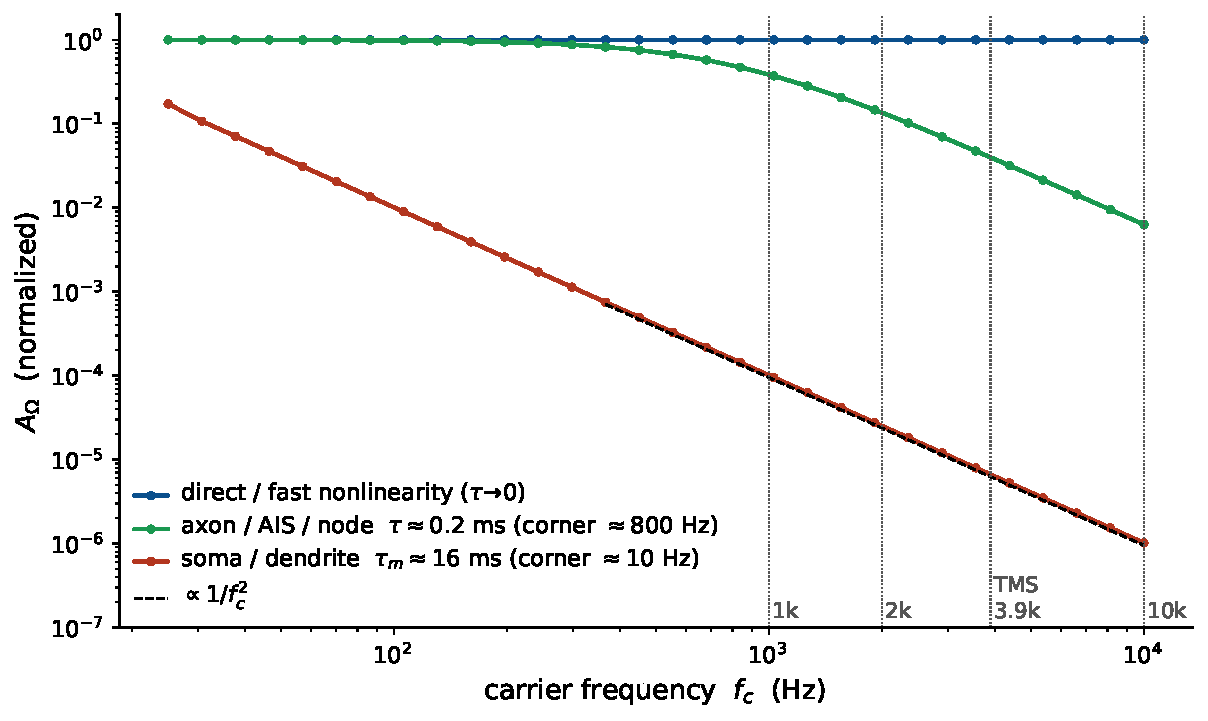
\includegraphics[width=0.74\textwidth]{fig_khz.pdf}
\caption{\DIFaddFL{\textbf{Carrier attenuation depends on the assumed access time (Jansen--Rit, open loop).} Open-loop
demodulated response (normalized to the $\tau\!\to\!0$ value) vs.\ carrier
frequency up to $10$~kHz. With direct coupling ($\tau\!\to\!0$) the response is
flat---carrier-independent. A slow somatic membrane ($\tau_m\!\approx\!16$~ms)
rolls off as $1/f_c^2$ (dashed guide); the assumed fast response
($\tau=0.2$~ms) retains about $0.14$ of the direct response at $2$~kHz and $0.04$
at $3.9$~kHz. These are sensitivity cases, not measurements of anatomical
compartments.}}
\label{fig:khz}
\end{figure}

\setcounter{figure}{5}
\begin{figure}[t!]
\centering
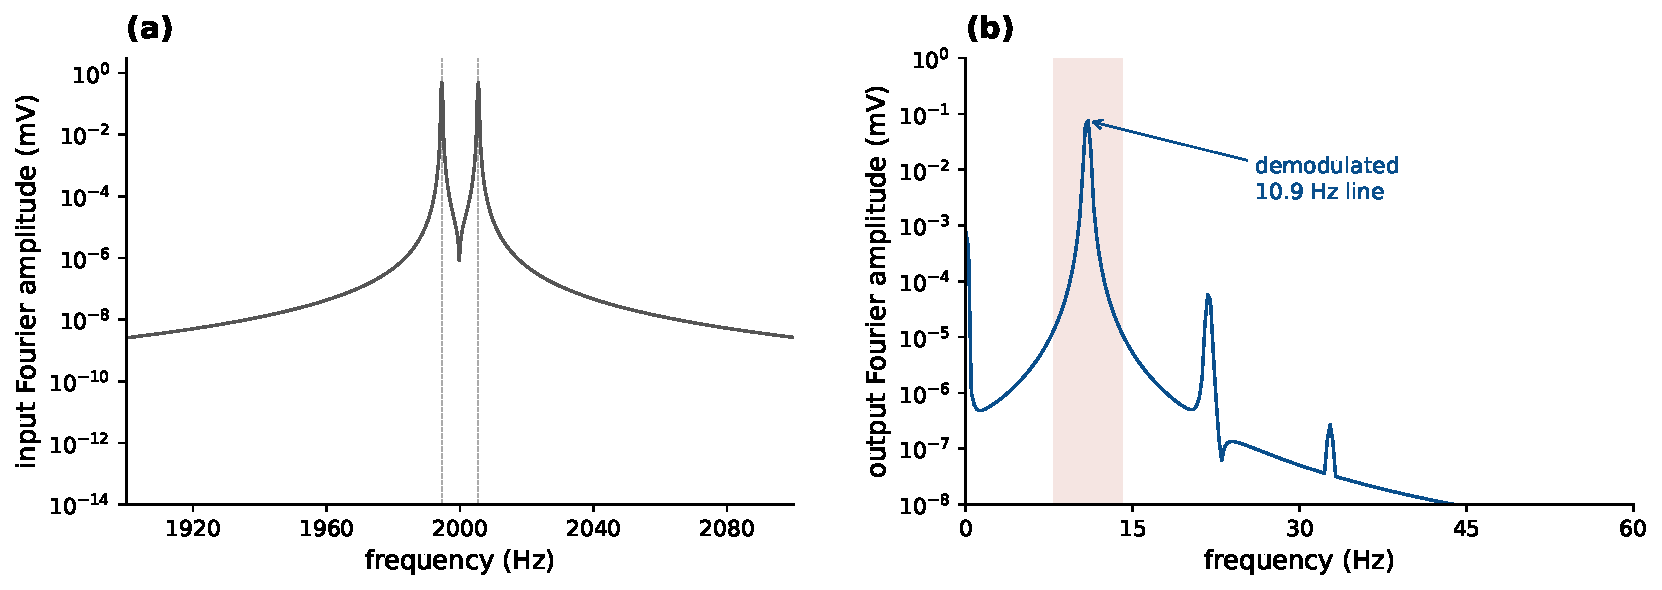
\includegraphics[width=0.95\textwidth]{fig_khz_twotone.pdf}
\caption{\DIFaddFL{\textbf{Two-tone TI at a kHz carrier (Jansen--Rit, assumed fast access).}
Two equal tones at $f_1=1994.543$ and $f_2=2005.457$~Hz, beating at
$10.914$~Hz, pass through the assumed low-pass ($\tau=0.2$~ms) into the recurrent column.
\emph{(a)} The input amplitude spectrum has lines only at $f_1$ and $f_2$; in the
$8$--$14$~Hz band its maximum is $2.2\times10^{-13}$~mV.
\emph{(b)} The output carries a demodulated line at the beat, $10.9$~Hz.}}
\label{fig:khz_twotone}
\end{figure}

\setcounter{figure}{8}
\begin{figure}[t!]
\centering
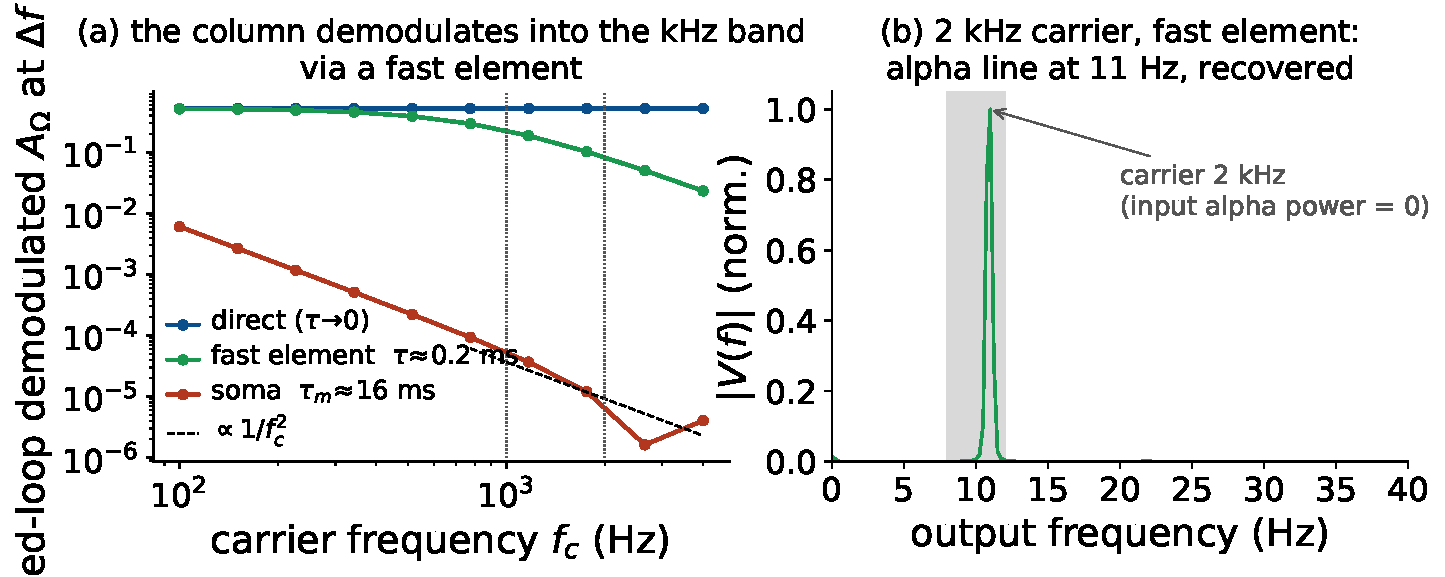
\includegraphics[width=\textwidth]{fig_khz_direct.pdf}
\caption{\DIFaddFL{\textbf{Demodulation at a kHz carrier (Jansen--Rit, closed loop).}
The applied field passes through an explicit membrane filter before the sigmoid.
\emph{(a)} Closed-loop demodulated $A_\Omega$ at $\Delta f=f_0$ vs.\ carrier $f_c$ for
three access models: direct ($\tau\!\to\!0$, carrier-independent), fast
($\tau=0.2$~ms), and somatic ($\tau_m=16$~ms; $1/f_c^2$ roll-off).
The fast time is assumed rather than assigned to a measured compartment.
\emph{(b)} Output spectrum for a
$2$~kHz carrier delivered through the fast element: an alpha line at $f_0$,
synthesized by the column although the input carries no alpha power.}}
\label{fig:khz_direct}
\end{figure}


\section{\DIFadd{Detection and harmonic signatures}}\label{supp:detection}
\DIFadd{These calculations support the carrier-scaling and harmonic tests in
\S\ref{sec:transduction} and the dynamic detector in \S\ref{sec:dynamic}.
}\subsection{\DIFadd{Fixed-voltage mixing and carrier exponents}}\label{supp:dynamic-details}
\DIFadd{Time and frequency use the membrane-time units defined in article
Appendix~\ref{app:mpr-coefficients}; $r^*,d,\nu$ have the same definitions.
Membrane access is already included in this calculation. The linear voltage response
is $H_v(\omega)=(i\omega+d)/[(i\omega+d)^2+\nu^2]$. Dividing by its squared magnitude
gives the mixing coefficient at fixed voltage excursion,
}\begin{equation}
\DIFadd{\kappa_V(Q,\omega)=\frac{\kappa_{\rm DC}(Q,\omega)}{|H_v(\omega)|^2}
=\frac{F'(Q)}{2}\;\frac{\omega^2+3d^2-\nu^2}{\omega^2+d^2}.
\label{eq:kfixed}
}\end{equation}
\DIFadd{This coefficient tends to $F'/2$ at high frequency. The $1/\omega^2$ suppression
at fixed current comes from $|H_v|^2$, the membrane filtering already represented
by }\ifsupp \DIFadd{main-text}\fi\DIFadd{\ Eq.~\eqref{eq:doors}; it is not an additional detector filter. A static curve
placed after the same membrane has the same leading carrier roll-off, although
its mixing coefficient and sign can differ. The steady-state curvature is
$F''=4r^*(3d^2-\nu^2)/(d^2+\nu^2)^3$, so the inflection occurs at $\nu^2=3d^2$.
}

\DIFadd{For nearby fast tones, the quadratic terms in }\ifsupp \DIFadd{main-text}\fi\DIFadd{\ Eq.~\eqref{eq:mpr} contribute at
different orders: $v^2$ at $\omega^{-2}$, $r v$ at $\omega^{-3}$, and $r^2$ at
$\omega^{-4}$. Table~\ref{tab:exponents} compares the carrier and beat routes to
the firing rate for a static curve and a dynamic population with the same membrane access.
}

\begin{table}[h]
\centering\small
\begin{tabular}{lcc}
\toprule
\DIFaddFL{stage }& \DIFaddFL{static curve, same membrane }& \DIFaddFL{dynamic population }\\
\midrule
\DIFaddFL{point-membrane current $\to$ voltage }& \DIFaddFL{$\omega^{-1}$ }& \DIFaddFL{$\omega^{-1}$ }\\
\DIFaddFL{voltage $\to$ rate, carrier }& \DIFaddFL{$1$ }& \DIFaddFL{$\omega^{-1}$ }\\
\DIFaddFL{current $\to$ rate, carrier }& \DIFaddFL{$\omega^{-1}$ }& \DIFaddFL{$\omega^{-2}$ }\\
\DIFaddFL{two tones $\to$ beat in the rate }& \DIFaddFL{$(\omega_1\omega_2)^{-1}$ }& \DIFaddFL{$(\omega_1\omega_2)^{-1}\times$ const. }\\
\bottomrule
\end{tabular}
\caption{\DIFaddFL{Fast-carrier scaling with matched point-membrane access, at fixed beat frequency
and a nonzero leading mixing coefficient. The dynamic population integrates the
carrier once more between voltage and rate; the beat is formed before that step.
Prefactors depend on the operating point and beat-frequency susceptibility.}}
\label{tab:exponents}
\end{table}

\DIFadd{The first row gives the shared membrane factor $1/\omega$. The second converts
voltage to rate: a static curve adds its slope, whereas the dynamic rate equation
integrates the carrier once more. Combining these stages gives the third-row
carrier responses, $\omega^{-1}$ and $\omega^{-2}$, respectively.
}

\DIFadd{The beat in the last row is formed before that additional rate integration:
static curvature and dynamic $v^2$ each mix the attenuated voltage, retaining
$(\omega_1\omega_2)^{-1}$. Equal exponents do not imply equal amplitudes; mixing
and the susceptibility at fixed $\Omega$ determine the prefactors. For the
uncoupled carrier-averaged response, $\kappa_V$ in Eq.~\eqref{eq:kfixed} tends to
$F'/2$, but is not the full finite-$\Omega$ network prefactor. Thus the dynamic
rate attenuates the carrier twice while forming the beat between those stages.
}

\ifjne
\subsection{\DIFadd{Harmonic ladder and mixed detectors}}\label{supp:harmonics}
\DIFadd{Envelope following and square-law detection are distinguishable at a single site. At a matched target,
$\mathcal A(t)=2\varepsilon|\cos(\Omega t/2)|$, whose Fourier series
$|\cos\theta|=\tfrac2\pi+\tfrac4\pi\sum_{n\ge1}\tfrac{(-1)^{n+1}}{4n^2-1}\cos(2n\theta)$ gives a
harmonic ladder whose nonnegative Fourier amplitudes $A_{n\Omega}$ obey $A_{2\Omega}/A_\Omega=1/5$, $A_{3\Omega}/A_\Omega=3/35$ and
$A_{4\Omega}/A_\Omega=1/21$. The square-law output $\half \mathcal A^2=\varepsilon^2(1+\cos\Omega
t)$ contains only DC and $\Omega$. For the mixed family $T(\mathcal A)=c_1\mathcal A+c_2\mathcal A^2$, with
$c_1\ne0$ and a nonzero fundamental, the
pre-network ratio is
}\begin{equation}
\DIFadd{\mathcal H_{\rm det}\equiv\left|\frac{Y_{2\Omega}}{Y_\Omega}\right|
=\frac{1/5}{\left|1+\tfrac{3\pi}{4}\,c_2\varepsilon/c_1\right|},
\label{eq:rdet}
}\end{equation}
\DIFadd{so measuring $\mathcal H_{\rm det}$ constrains $c_2\varepsilon/c_1$ within this family.}\footnote{\DIFadd{The inverse has two branches unless the sign of the fundamental
relative to the linear term is known; for $c_2/c_1\ge0$ it is unique.}}

\fi
\subsection{\DIFadd{AM-surrogate and genuine two-tone comparisons}}\label{supp:waveform-checks}
\DIFadd{These checks support the waveform choices in \S\ref{sec:waveforms}. Agreement
at the leading beat does not imply equal steady sources or driven operating states.
}

\begin{table}[htbp]\centering\small
\caption{\DIFaddFL{Waveform comparisons at the stated operating points. JR response ratios
use the same voltage readout; timing ratios use the same pyramidal firing rate.}}
\label{tab:waveform-checks}
\begin{tabular}{@{}p{4.3cm}p{4.5cm}p{6cm}@{}}
\toprule
\DIFaddFL{Comparison }& \DIFaddFL{Conditions }& \DIFaddFL{Result}\\
\midrule
\DIFaddFL{JR open-loop beat }& \DIFaddFL{$v^*=8$ mV }& \DIFaddFL{Two-tone/AM: $1.0000$ at $0.02$ mV; $0.988$ at $1$ mV.}\\
\DIFaddFL{JR modulation/mean shift }& \DIFaddFL{Pinned sweep: far from Hopf, $\gamma=1$ s$^{-1}$, nearest point }& \DIFaddFL{Two tones: $14.5$, $58$, $44$; AM: $19$, $66$, $45$. AM has $3/4$ of the two-tone direct steady source.}\\
\DIFaddFL{JR TI/tACS output }& \DIFaddFL{Far from Hopf, $\gamma=1.07$ and $0.12$ s$^{-1}$ }& \DIFaddFL{AM: $0.14$, $0.24$, $0.47$; two tones: $0.14$, $0.24$, $0.46$. Difference at most $2.2\%$ across the grid.}\\
\DIFaddFL{JR matched-source output }& \DIFaddFL{Three couplings, settings in \S\ref{app:jr-sweep-settings} }& \DIFaddFL{TI/tACS: $0.99$, $0.94$, $0.92$ for AM; $0.99$, $0.93$, $0.90$ for two tones.}\\
\DIFaddFL{PING beat }& \DIFaddFL{Well below Hopf; $\bar\eta=0.9$ }& \DIFaddFL{Matched AM and two-tone responses agree within $0.07\%$ and $4\%$, respectively.}\\
\bottomrule
\end{tabular}
\end{table}

\subsection{\DIFadd{The cubic Hopf normal form lacks a quadratic mixer}}\label{app:sl}
\DIFadd{The Stuart--Landau equation \cite{pikovsky2001}
}\begin{equation}
\DIFadd{\dot z=(\alpha+i\omega_0)z-|z|^2z+\mathcal F(t),\qquad
\gamma=-\alpha>0,
\label{eq:sl}
}\end{equation}
\DIFadd{uses seconds for time and a normalized complex mode $z$, with the cubic
coefficient set to $1$~s$^{-1}$. Its linear growth rate is $\alpha=-\gamma$;
$\gamma$ has units s$^{-1}$. The mode has damping $\gamma$ and natural angular frequency
$\omega_0$, driven by the applied input $\mathcal F$ (normalized mode units per second). For a weak input
$\mathcal F=\varepsilon_{\rm SL} \psi_{\rm SL}(t)$ with dimensionless waveform $\psi_{\rm SL}$ on the stable side, the perturbative response has
the form $z=\varepsilon_{\rm SL} z_1+\varepsilon_{\rm SL}^3z_3+\cdots$. There is no second-order
source: the first-order response contains only the applied frequencies, and the
cubic first contributes at order $\varepsilon_{\rm SL}^3$. Thus the normal form has a
resonant linear susceptibility but lacks the quadratic difference-frequency
generation of }\ifsupp \DIFadd{main-text}\fi\DIFadd{\ Eq.~\eqref{eq:demod}. This statement concerns the weak-input
expansion; it is not an exclusion of every higher-order intermodulation or
strong-drive response.
}

\DIFadd{In the numerical control ($\alpha=-0.5$~s$^{-1}$, $f_0=10$~Hz, $f_c=100$~Hz,
$\varepsilon_{\rm SL}=0.5$~s$^{-1}$), a square-law detector gives a beat-frequency lock-in amplitude
of $2.5\times10^{-1}$, while $\mathrm{Re}\,z$ gives approximately
$2\times10^{-8}$, at the numerical floor. Driving the same mode directly in band
recovers the forced $1/\gamma$ growth. The control separates resonant amplification
from the nonlinear source required to drive it at the beat.
}

\section{\DIFadd{Spatial maps}}\label{supp:spatial}
\DIFadd{These definitions and checks support the geometric maps in \S\ref{sec:fem-results}
and the interpretation of mean-square polarization in \S\ref{sec:dc}.
}\ifjne
\subsection{\DIFadd{Envelope-mean subharmonicity}}\label{supp:envelope-proof}
\DIFadd{The envelope mean has the same restriction. At each beat phase $\vartheta$,
$\mathcal A$ is the Euclidean norm of
$(\varepsilon_1+\varepsilon_2\cos\vartheta,\,\varepsilon_2\sin\vartheta)$,
a vector of harmonic functions. A norm is convex, so this envelope is subharmonic;
averaging over $\vartheta$ preserves that property. Thus both idealized mean maps
lack a strict interior maximum under these conditions (Fig.~\ref{fig:spatial_maps}b).
}

\subsection{\DIFadd{Isotropic orientation averages}}\label{supp:orientation}
\DIFadd{For isotropically distributed unit orientations
$\mathbf n$ with orientation-independent access and curvature,
$\langle(\mathbf n\cdot\mathbf E_j)^2\rangle=|\mathbf E_j|^2/3$
and $\langle(\mathbf n\cdot\mathbf E_1)(\mathbf n\cdot\mathbf E_2)\rangle
=\mathbf E_1\cdot\mathbf E_2/3$: orthogonal fields cancel the averaged beat,
but retain the DC intensity.
}

\fi
\ifjne
\subsection{\DIFadd{Head-model procedure}}\label{supp:fem-protocol}
\DIFadd{To compare the spatial predictions on the same anatomy, we compute all maps
in one open-access subject,
IXI002 of the IXI dataset}\footnote{\url{https://brain-development.org/ixi-dataset/}}
\DIFadd{(T1-weighted MRI; female, 35 years). The T1 image was segmented into six tissues
(scalp, skull, cerebrospinal fluid, gray matter, white matter and eyes) and meshed with
SimNIBS~3.2.3 \texttt{headreco} \cite{nielsen2018}, with its CAT12 option
\cite{gaser2024}. Tissue conductivities were 0.33 (scalp), 0.008 (skull), 1.79
(cerebrospinal fluid), 0.40 (gray matter), 0.15 (white matter) and 0.33~S/m (eyes)
\cite{salvador2025}. These are low-frequency values; no dispersion correction was
applied at the kHz carriers. The volume conductor is linear and quasi-static, so the
carrier frequencies do not enter the maps.
}

\DIFadd{The electrodes follow the published hippocampal montage of Violante et al.\
\cite{violante2023}, placed by its recipe on the subject's registered 10--10
positions. Pair~1 (anterior) joins e1, 25~mm from T9 toward FT9, to e2, 10~mm from AF8
toward Fp2. Pair~2 (posterior) joins e3, 25~mm from T9 toward TP9, to e4, 10~mm from P8
toward PO8. Each electrode is a 20-mm disc of 3~mm of gel (4.0~S/m) under 2~mm of metal
(10~S/m), meshed into the head model with SimNIBS~3.2.3; the resulting mesh has
$3.64\times10^6$ linear tetrahedra. As a montage sensitivity, the 10--10 rendering of
this montage, FT7--F8 (anterior) and TP7--P8 (posterior), which Yatsuda et al.\
\cite{yatsuda2024} used as their starting montage, was meshed and solved in the same
way. Each montage has its own mesh, carrying only its own four electrodes.
}

\DIFadd{Each pair was solved once at 1~A. The potential $\phi_j$ (V) satisfies
$\nabla\!\cdot\!(\sigma_{\rm cond}\nabla\phi_j)=0$, where
$\sigma_{\rm cond}$ is tissue conductivity (S/m). Current enters and leaves through each
electrode's metal contact as a Neumann condition, distributed in proportion to nodal
area; the rest of the scalp carries no normal current, and one pinned node fixes the
gauge. The linear finite-element system was assembled and solved with Neuroelectrics'
temporal-interference library, by conjugate gradients with algebraic-multigrid
preconditioning, to a relative residual of $10^{-8}$. The field
$-\nabla\phi_j$ was recovered at gray- and white-matter
nodes by superconvergent patch recovery \cite{zienkiewicz1992}, separately within each
compartment (446}{\DIFadd{,}}\DIFadd{877 node--compartment pairs). Dividing these fields by the solve
current gives the field-per-current vectors $\mathbf F_j$, expressed in
(V/m)/mA to match $I_j^{\rm pair}$. Every current condition is a scaling of these two fields.
With peak pair currents $I_1^{\rm pair}$ (anterior) and
$I_2^{\rm pair}$ (posterior) summing to 4~mA, the ratio 1:1 is $2+2$~mA and 1:3 is
1~mA anterior plus 3~mA posterior, the two conditions of Violante et al. The ratio sweep
sets the posterior share $I_2^{\rm pair}/(I_1^{\rm pair}+I_2^{\rm pair})$ from 0.1 to
0.9 in steps of 0.025.
}

\DIFadd{The field-to-polarization conversion follows \S\ref{sec:envelope}:
$\varepsilon_j(\mathbf x)=I_j^{\rm pair}\mathcal P_j(\mathbf x)$, with
$\mathcal P_j=\lambda_0\,\mathbf F_j\!\cdot\!\mathbf n$, one uniform
static coupling $\lambda_0=0.5$~mV per V/m \cite{radman2009}, and
$\lambda_f\approx\lambda_0$. A uniform coupling multiplies the envelope map by
$\lambda_0$ and the two second-order maps by $\lambda_0^2$. Target-to-reference ratios,
normalized maps and focus positions do not depend on it. Hippocampal couplings of
$0.12$--$0.18$~mV per V/m \cite{bikson2004,deans2007} would scale the absolute values
by $0.24$--$0.36$ and $0.06$--$0.13$, respectively.
}

\DIFadd{The detector compartment fixes the projection direction. A laminar direction for a pyramidal
axon initial segment, a local axon direction for a node, or an orientation
distribution for terminals defines a different access model. Isotropic averaging
is one possible distribution, not an anatomical consequence of choosing terminals.
Maximizing a geometric map over orientation gives an upper bound for that map
at each location; it does not identify the detector's orientation.
}

\DIFadd{The projection direction $\mathbf n(\mathbf x)=\mathbf n^*(\mathbf x)$ is the envelope-maximizing direction at
the reference ratio 1:1: the closed-form maximizer, over unit vectors, of
$2\min(|\mathbf F_1\!\cdot\!\mathbf n|,|\mathbf F_2\!\cdot\!\mathbf n|)$
\cite{grossman2017}. It is chosen once at each node and then held fixed for 1:1, 1:3
and every ratio of the sweep, and all three maps use it. Along it, the 1:1 envelope map
equals its maximum over orientation. At any other ratio it is the envelope seen by an
element with that fixed orientation, which can be below that ratio's own maximum. As an
orientation sensitivity, every statistic was repeated along a second fixed field, the
radial direction from the brain centroid. The isotropic comparison averages the signed
mixing term over uniformly distributed orientations before its magnitude is taken:
$\langle\varepsilon_1\varepsilon_2\rangle_{\mathbf n}
=\lambda_0^2I_1^{\rm pair}I_2^{\rm pair}\,\mathbf F_1\!\cdot\!\mathbf F_2/3$, so the
isotropic beat excursion is
$\tfrac23\lambda_0^2I_1^{\rm pair}I_2^{\rm pair}|\mathbf F_1\!\cdot\!\mathbf F_2|$.
Elements whose beats have opposite phase cancel in this average.
}

\DIFadd{The target is the left hippocampus of a FreeSurfer~6.0.0 \texttt{recon-all}
segmentation of the same T1 image (\texttt{aseg} label 17, 3903~mm$^3$)
\cite{fischl2002}. The region of interest (ROI) is the 1}{\DIFadd{,}}\DIFadd{568 gray- and white-matter
nodes inside it. The reference is the 273}{\DIFadd{,}}\DIFadd{544 gray-matter nodes outside the
ROI, including other deep gray matter. It is a gray-matter reference, not a cortex-only contrast.
The mesh and the segmentation share one image frame; tissue-volume, centroid and
white-matter checks confirmed their alignment. As a label sensitivity, the
Neuromorphometrics atlas hippocampus, warped into the subject with SimNIBS~3.2.3
\texttt{mni2subject} and the subject's nonlinear MNI transform (1}{\DIFadd{,}}\DIFadd{345 nodes; Dice 0.72
with the FreeSurfer label), replaced the ROI. As a tissue sensitivity, the ROI was
restricted to its gray-matter nodes (1}{\DIFadd{,}}\DIFadd{174 with the FreeSurfer label, 1}{\DIFadd{,}}\DIFadd{013 with
the atlas label).
}

\DIFadd{The target-to-reference ratio is the ROI 95th percentile divided by the reference
95th percentile; its mean-based companion divides the ROI mean by the same
reference percentile. All percentiles and centroids weight nodes equally.
The quadratic excursion and $\mathcal I$ are second order in the field, whereas
the envelope excursion is first order. To separate this difference in degree
from the spatial weighting, each second-order statistic is also given
degree-matched, computed on the square root of the map. This is a geometric
comparison; the raw maps remain the respective detector predictions before gain.
The focus is the centroid of the top 10\% of ROI nodes,
ranked by the map's own value, with 5, 25 and 50\% as a sensitivity. Ranking makes the
focus exactly invariant to a uniform positive factor. Its displacement from 1:1 is
measured along the hippocampal long axis, the first principal axis of the ROI nodes,
with anterior positive. Field projections still use $\mathbf n^*$, independently
of this reporting axis. The 1:1 to 1:3 displacement was computed for every combination
of montage, label, ROI tissue definition and focus fraction (32 per map), each montage
along its own 1:1 direction.
}

\DIFadd{No signed DC-source or mean-response map is computed. For a spatially uniform detector
coefficient, $Y_{\rm DC}=\tfrac12\Sig''(v^*)\mathcal I$ (\S\ref{sec:dc}) is
$\mathcal I$ rescaled, with the sign of $\Sig''(v^*)$. A nonuniform coefficient would
require an operating-point map, which a head model does not provide, and a mean
response would additionally require a circuit model. In particular,
$\Sig''(v^*)$ is curvature at the population model's operating point, not a
measurement of the transfer at the axon initial segment. Assigning that
coefficient to an anatomical detector requires a calibrated access and
input--output model.
}

\subsection{\DIFadd{Sensitivity of focus displacement}}\label{supp:fem-sensitivities}
\DIFadd{The spatial ordering in the article persists across montage, labeling, tissue,
and focus-fraction choices. Table~\ref{tab:fem-sensitivities} gives the ranges;
orientation changes absolute contrast more than the atlas label in this subject.
For the reference projection and label, the top-5--50\% focus moves
$2.2$--$4.0$~mm anteriorly for the envelope and $2.4$--$8.2$~mm posteriorly
for mean-square polarization.
}

\begin{table}[htbp]\centering\small
\caption{\DIFaddFL{Focus displacement from 1:1 to 1:3. Envelope shifts are anterior;
mean-square shifts are posterior. The quadratic beat shift is zero in every case.
Contrasts quoted in the last column are raw 1:1 envelope/quadratic contrasts.}}
\label{tab:fem-sensitivities}
\begin{tabular}{@{}lrrl@{}}
\toprule
\DIFaddFL{Sensitivity }& \DIFaddFL{Envelope (mm) }& \DIFaddFL{Mean square (mm) }& \DIFaddFL{Contrasts}\\
\midrule
\DIFaddFL{Atlas label }& \DIFaddFL{$2.0$--$3.8$ }& \DIFaddFL{$3.2$--$5.9$ }& \DIFaddFL{$1.17$ / $1.04$}\\
\DIFaddFL{Radial direction }& \DIFaddFL{$1.9$--$2.8$ }& \DIFaddFL{$2.0$--$3.7$ }& \DIFaddFL{$1.62$ / $1.97$}\\
\DIFaddFL{All 32 combinations }& \DIFaddFL{$0.7$--$8.1$ }& \DIFaddFL{$0.5$--$10.6$ }& \\
\bottomrule
\end{tabular}
\end{table}

\subsection{\DIFadd{Mean-square change under current-ratio steering}}\label{supp:steering-algebra}
\DIFadd{The mean-square polarization
changes by $\mathcal I_{1:3}/\mathcal I_{1:1}
=(\mathcal P_1^2+9\mathcal P_2^2)/[4(\mathcal P_1^2+\mathcal P_2^2)]$,
exceeding one only where $|\mathcal P_2|>\sqrt{3/5}|\mathcal P_1|
\approx0.775|\mathcal P_1|$. Its hippocampal mean rises by 24\% and its focus
moves 4.5~mm posteriorly. Equal summed currents therefore do not match local
RMS polarization.
}

\fi
\setcounter{figure}{12}
\begin{figure}[t!]
\centering
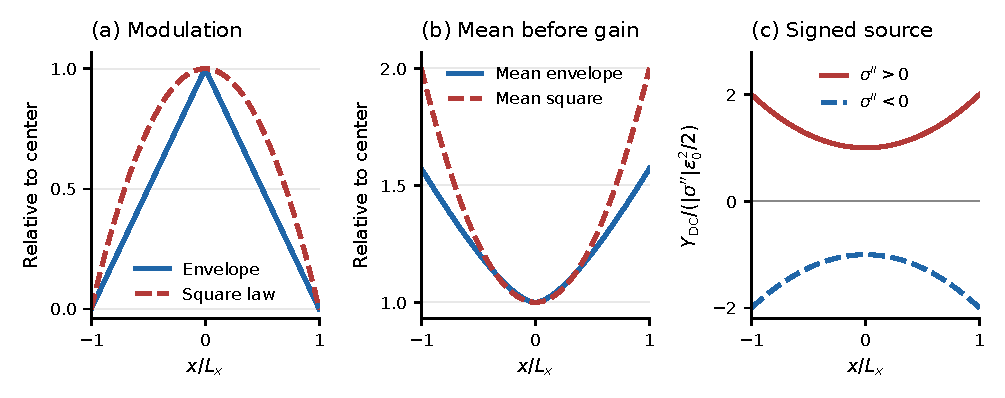
\includegraphics[width=\textwidth]{fig_spatial_maps.pdf}
\caption{\DIFaddFL{\textbf{Envelope and quadratic spatial maps.} Illustrative line profile:
$\varepsilon_1(x)=\varepsilon_0(1+x/L_x)$ and
$\varepsilon_2(x)=\varepsilon_0(1-x/L_x)$ on $-L_x\le x\le L_x$, with polarization scale
$\varepsilon_0>0$ (mV) and length $L_x>0$ (m). In (a,b), each geometric curve is
divided by its own positive value at $x=0$.
\emph{(a)} Modulation is $1-|x/L_x|$ for envelope following and $1-(x/L_x)^2$ for quadratic
detection: both peak centrally, but the quadratic profile is broader here.
\emph{(b)} The mean envelope and mean-square polarization $\mathcal I$ both
increase toward the edges; neither includes a signed detector gain.
\emph{(c)} The static JR rate source $Y_{\rm DC}=\Sig''\mathcal I/2$ for uniform
positive curvature (solid red) or negative curvature of the same magnitude
(dashed blue). Both use the same positive scale $|\Sig''|\varepsilon_0^2/2$,
giving $\pm[1+(x/L_x)^2]$; the gray line marks zero. These are assumed detector
states before recurrent feedback, not inferred physiological responses.
This is a line profile, not a head model or a demonstration of three-dimensional focusing.}}
\label{fig:spatial_maps}
\end{figure}


\section{\DIFadd{Recurrent amplification and numerical checks}}\label{supp:amplification}
\DIFadd{These protocols support the coupling, timing, and field-induced gamma results in
\S\ref{sec:jcurve}--\S\ref{sec:qif}.
}\subsection{\DIFadd{JR coupling-sweep settings}}\label{app:jr-sweep-settings}
\DIFadd{The coupling sweeps of Figs.~\ref{fig:jcurve} and~\ref{fig:timing}, and the transcranial
alternating-current stimulation (tACS) control of Fig.~\ref{fig:tacs}, use the single JR
column with the field-free operating point $v^*$ pinned: for
each global connectivity $C$ we solve the field-free fixed-point relation analytically
for the external drive $p(C)$ that holds $v^*$ (hence $\Sig''(v^*)$) fixed, vary $C$
toward the alpha Hopf, and read $\gamma,\omega_0$ from the $6\times6$ Jacobian. The field
is the AM surrogate of }\ifsupp \DIFadd{main-text}\fi\DIFadd{\ Eq.~\eqref{eq:amsur} for Fig.~\ref{fig:jcurve}, genuine two
tones for the timing comparison (Fig.~\ref{fig:timing}), or a direct in-band sinusoid $s(t)=\varepsilon\cos\Omega t$
($\varepsilon=0.1$~mV) for the tACS control (Fig.~\ref{fig:tacs}), each read out by the
lock-in of $v$ at $\Delta f$, except in the timing comparison, which reads the
modulation and mean of the same pyramidal rate $r_P=\Sig(v+s)$.
That comparison uses $18$~s settling and a $20$~s window for each waveform.
The Figure~\ref{fig:jcurve}--Figure~\ref{fig:tacs} response-ratio comparison uses
$v^*=8.30$~mV, TI surrogate amplitude $0.3$~mV with $m=1$ and $f_c=100$~Hz,
and tACS amplitude $0.1$~mV, driven at each field-free modal frequency.
The original TI amplitudes are interpolated logarithmically in $C$ onto the tACS
grid. For the waveform comparison, both the surrogate and two-tone TI are rerun
on that grid with $12$~s settling and a $6$~s window.
Pinning fixes the background curvature; it does not cancel the stimulation-induced
mean shift.
Additional controls at $C=110$, $133.9091$, and $136.3$ use a tACS amplitude of
$0.0143039$~mV, matched to the leading TI beat source. They record mean voltage,
mean rate, and lock-in with $12$~s settling and a $6$~s window, repeated with
$60$~s settling and a $20$~s window; the latter settings also test genuine two tones.
}


\subsection{\DIFadd{Stability of the driven PING endpoint}}\label{app:ping-stability}
\DIFadd{We check the stability of the driven $J$-curve endpoint by integrating the full
variational matrix along its trajectory. At carrier $300$~Hz and beat $50.5$~Hz,
the AM input repeats every $2$~s. After $8$~s of settling, we compute the
perturbation multipliers over that period and repeat over the next period.
Moduli below one indicate decay of perturbations to the periodic response.
Two-tone controls at $J=16.5663$ and $16.5901$, both with a $50.5$~Hz beat,
use $5$~s settling, direct perturbation decay, and an $8$~s finite-time
Lyapunov estimate.
}

\DIFadd{Although a DC-only averaged calculation predicts an unstable endpoint, the full
periodically forced solution remains attracting: its largest perturbation
multiplier is $0.034$ over the $2$~s forcing period. Increasing settling from
$0.6$ to $3$~s changes the endpoint lock-in by $0.8\%$. With genuine two tones,
the $50.5$~Hz endpoint control also attracts nearby trajectories: perturbations
decay at $-0.0014$~ms$^{-1}$, and the $8$~s Lyapunov estimate is
$-0.00079$~ms$^{-1}$. These controls test a nonlinear driven response, not linear
gain about the DC-shifted equilibrium.
}

\subsection{\DIFadd{Finite-network numerical checks}}\label{app:qif-checks}
\DIFadd{At $A_f=10$ and $\bar\eta=0.85$, the finite-network beat depth is $0.093$
for the published cutoff, versus the mean-field value $0.128$. Raising the spike cutoff from $V_{\rm peak}=100$ to
$200$ and $400$ gives depths $0.127$ and $0.139$, while the mean-rate increase
stays at $2.8$--$2.9\%$. At the original cutoff, doubling the population gives
$0.083$ and halving the time step gives $0.093$. The response is therefore
sensitive to the finite spike cutoff. Halving the step at cutoffs $200$ and
$400$ gives depths $0.121$ and $0.141$, respectively: cutoff dependence persists,
and quantitative convergence remains unestablished at this population size.
At the plotted cutoff, the pooled spike-phase vector strength is $0.046$;
median per-neuron phase consistency remains negative in field-off and field-on
windows at all three cutoffs.
In the $A_f=35$ convergence checks, halving the time step changes the lock-in and the pooled vector
strength by under $1\%$; doubling the spike-detection threshold changes the lock-in by
about $1\%$ and the mean rate by $2\%$, but the pooled vector strength at
$\bar\eta=0.85$ by about $45\%$, so phase concentration, unlike rate modulation, is sensitive to
how spike times are defined.
}


\subsection{\DIFadd{Fast-carrier estimate at the illustrated amplitudes}}
\DIFadd{The $A_f=35$ runs are finite-amplitude illustrations: the fast-carrier estimate gives a voltage excursion
$A_f/(\tau_E\omega_c)\approx1.2$ per tone in the model's voltage units. Its
rectified excitatory-drive shift is about $1.5$, compared with $0.12$ at
$A_f=10$. At $\bar\eta=0.85$, the Hopf threshold for a drive shift applied
only to the excitatory population is $\delta\eta_E^*\approx0.286$. The larger
field is therefore expected to cross this threshold, whereas the smaller one
remains below it.
}

\setcounter{figure}{2}
\begin{figure}[t!]
\centering
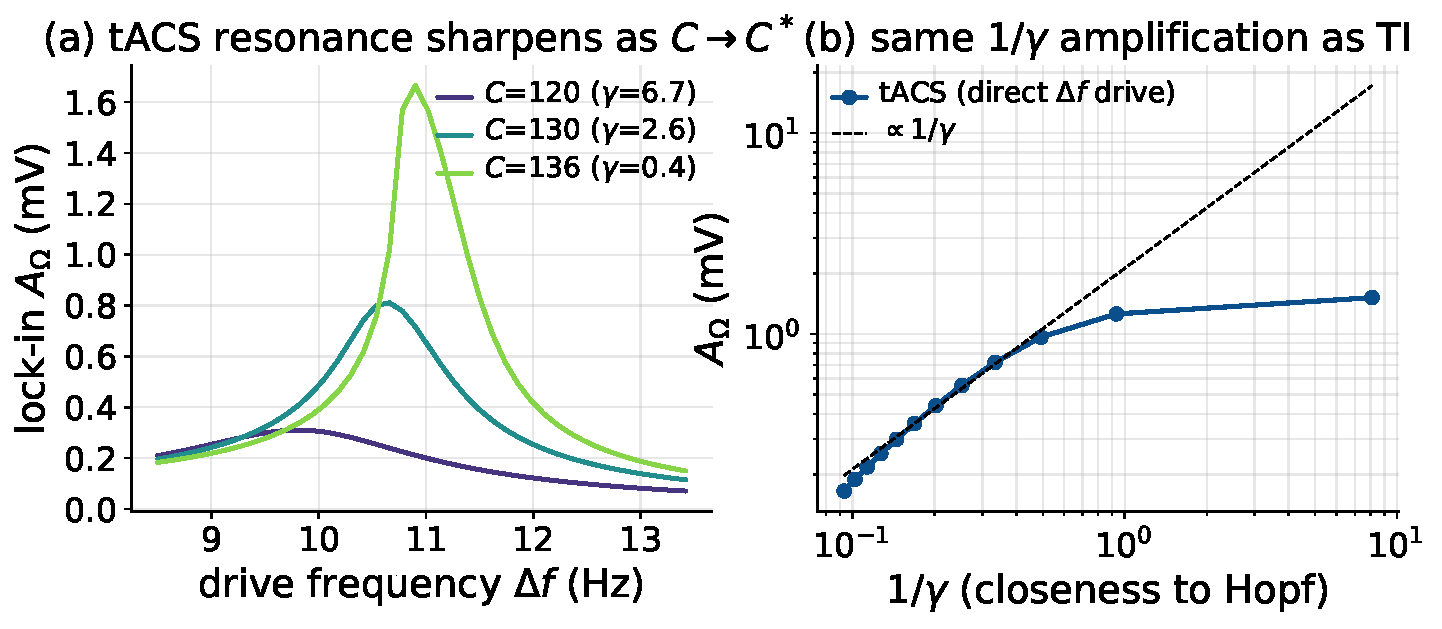
\includegraphics[width=0.92\textwidth]{fig_tacs_jcurve.pdf}
\caption{\DIFaddFL{\textbf{tACS shares the network amplifier (Jansen--Rit).} A direct
low-frequency (tACS) drive at $\Delta f$ enters the column without a carrier, so it
needs no demodulation, but feeds the same near-Hopf resonator. With the field-free operating point
pinned, sweeping the coupling $C$ toward the alpha Hopf: \emph{(a)} the lock-in
resonance at $\Delta f$ sharpens and grows as $C\!\to\!C^*$; \emph{(b)} the response
grows as $1/\gamma$ (dashed) and saturates near criticality---the same network
amplification as the demodulated TI drive (Fig.~\ref{fig:jcurve}). The leading tACS
response is linear in the field; the TI beat is quadratic. Their response ratio
is independent of damping in linear response and changes at the finite amplitudes
nearest the Hopf (\S\ref{sec:jcurve}). Here $\gamma>0$ describes the field-free state.}}
\label{fig:tacs}
\end{figure}

\setcounter{figure}{3}
\begin{figure}[t!]
\centering
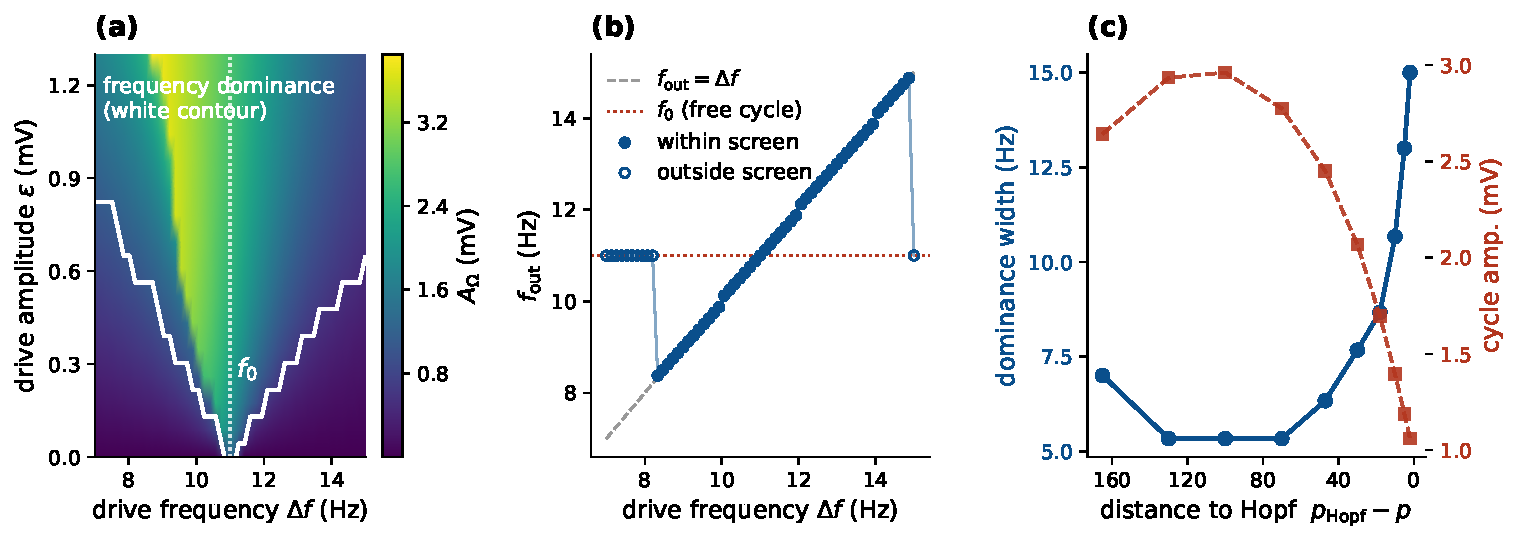
\includegraphics[width=\textwidth]{fig_entrainment.pdf}
\caption{\DIFaddFL{\textbf{Frequency dominance in the driven autonomous Jansen--Rit column.}
The column is set in its autonomous alpha limit cycle ($p=250$, $f_0\!\approx\!11$~Hz) and
driven by a direct in-band sinusoid. \emph{(a)} The set
$|f_{\rm out}-\Delta f|<0.3$~Hz forms a wedge near $f_0$ that widens with drive.
It screens for phase capture but does not establish it. \emph{(b)} Inside this
region the dominant frequency follows $\Delta f$; outside, it remains near $f_0$.
\emph{(c)} Toward the Hopf at fixed drive the dominance width grows as the
autonomous cycle amplitude vanishes (blue, left axis; red dashed, right axis). Above the
Hopf this width describes frequency selection in a driven autonomous oscillator;
it is distinct from the linear susceptibility of the stable-focus side
(Fig.~\ref{fig:jcurve}). Both diagnostics increase toward criticality in these sweeps.}}
\label{fig:entrain}
\end{figure}

\setcounter{figure}{7}
\begin{figure}[t!]
\centering
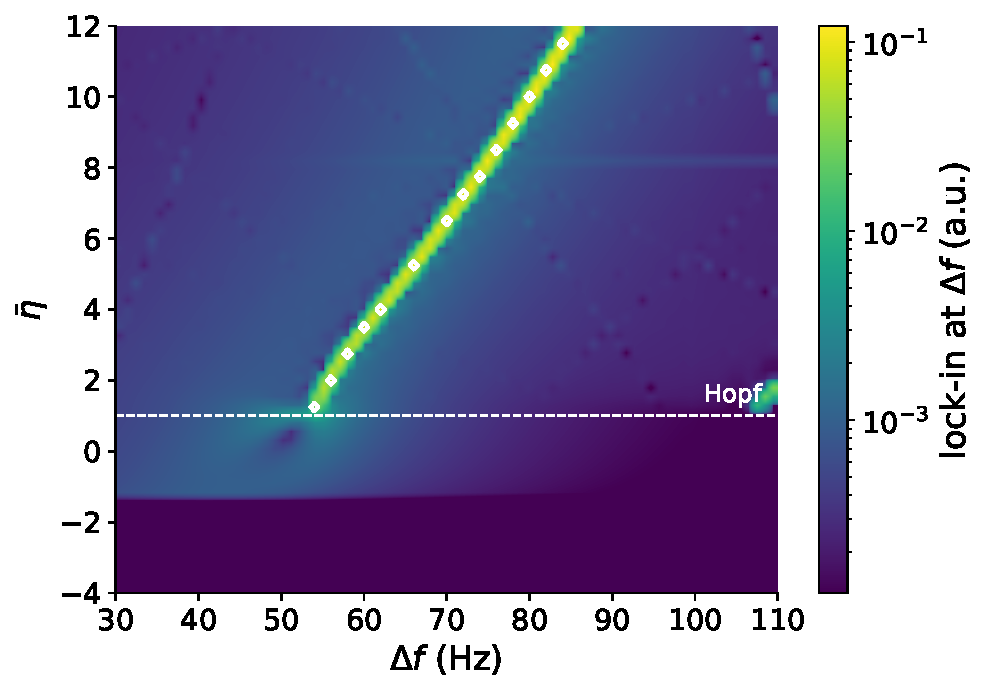
\includegraphics[width=0.72\textwidth]{fig_nmm2_map.pdf}
\caption{\DIFaddFL{\textbf{NMM2 PING resonance map (exact mean field).} Demodulated response over
the ($\Delta f$, background drive $\bar\eta$) plane, log color scale. The ridge follows the
gamma natural frequency, with $f_0$ rising with $\bar\eta$ for these parameters. White markers
outline the frequency-dominance set (\S\ref{sec:vocab}), drawn only above the Hopf
(dashed line) where there is an autonomous rhythm to capture; below it the same color field
is a forced response. The markers do not establish phase capture. Lock-in amplitude
cannot separate driven and autonomous contributions, since both can place power at
$\Delta f$.}}
\label{fig:nmm2_map}
\end{figure}

\setcounter{figure}{9}
\begin{figure}[t!]
\centering
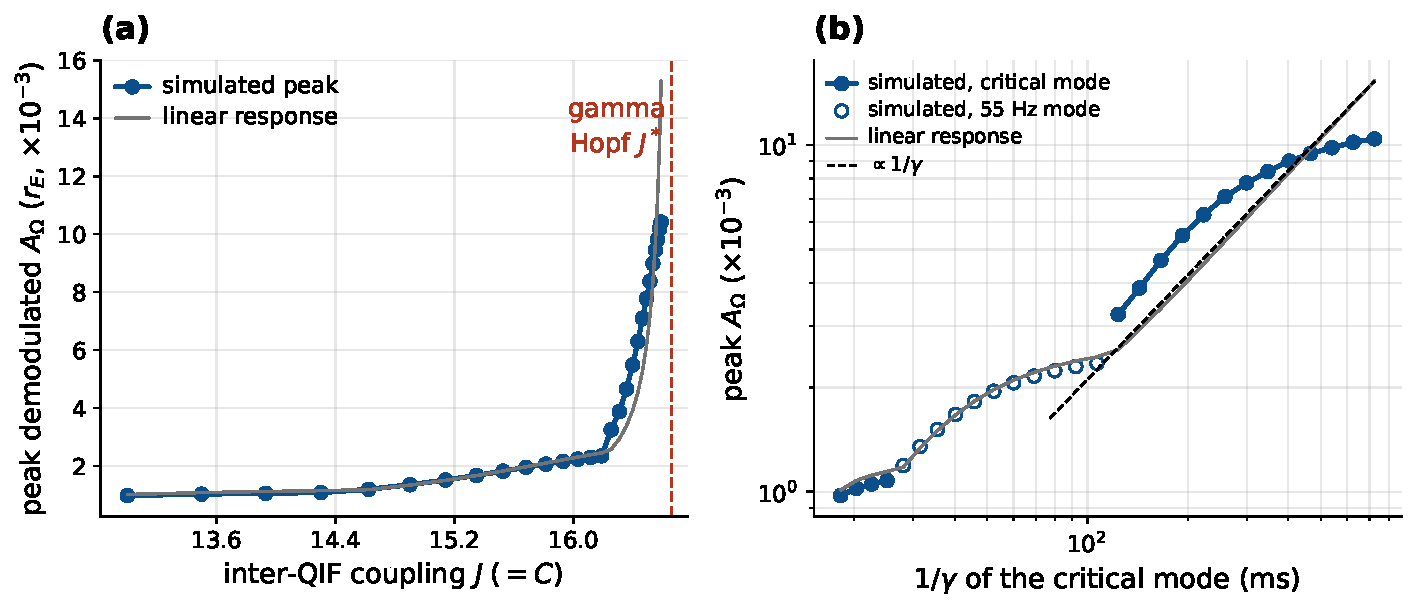
\includegraphics[width=0.92\textwidth]{fig_nmm2_jcurve.pdf}
\caption{\DIFaddFL{\textbf{Coupling changes the dominant mode and its gain in NMM2.}
Unpinned sweep at $\bar\eta=0$, AM surrogate $A_f=8$.
\emph{(a)} Simulated rate peak (blue) and linear reference including the
second-order source (gray), normalized over $14.5<J<16$. Red dashed:
field-free Hopf. \emph{(b)} Gain against inverse damping of the critical
mode. Filled symbols: that mode carries the linear peak; open symbols:
the competing $55$~Hz mode carries it ($14.6\lesssim J\lesssim16.2$).
The dashed $1/\gamma$ guide is anchored at the last linear point.
The simulation exceeds then falls below the guide. The driven endpoint
remains attracting under both AM and genuine two-tone forcing.}}
\label{fig:nmm2_jcurve}
\end{figure}

\setcounter{figure}{10}
\begin{figure}[t!]
\centering
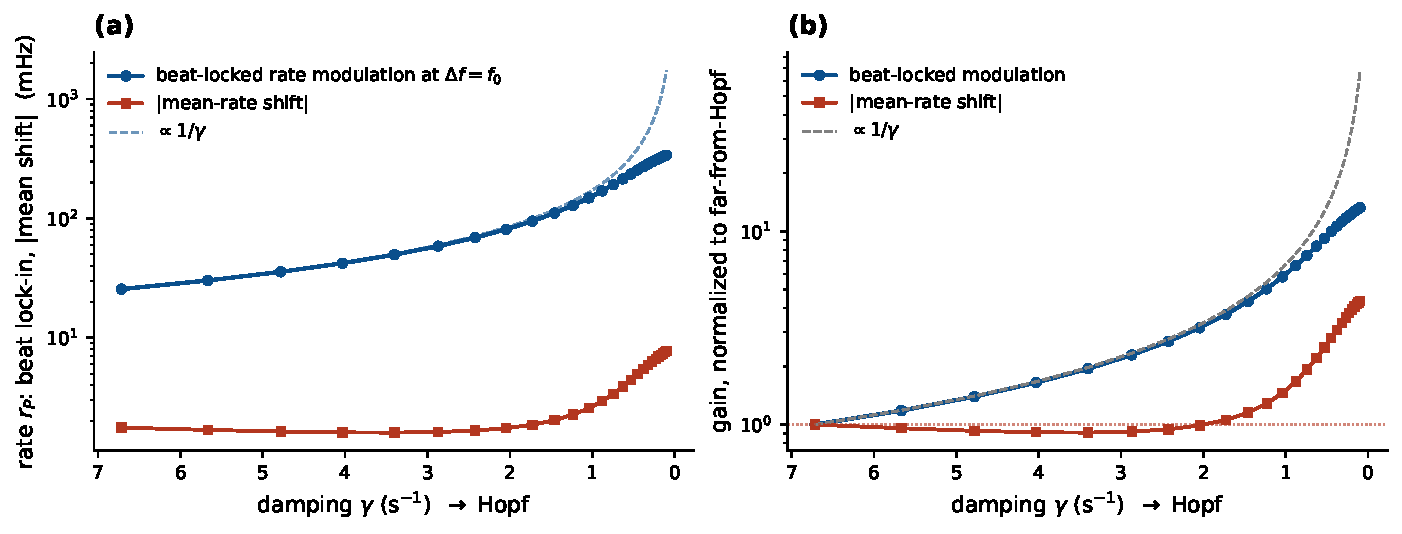
\includegraphics[width=\textwidth]{fig_timing_not_rate.pdf}
\caption{\DIFaddFL{\textbf{Beat modulation grows more than the mean-rate shift.}
JR coupling sweep with fixed field-free curvature and genuine two-tone
input, $\Delta f=f_0$. Both observables use the pyramidal rate
$r_P=\Sig(v+s)$, in mHz.
\emph{(a)} Beat amplitude (blue) follows $1/\gamma$ (dashed) before
saturating; mean-shift magnitude (red) remains smaller.
\emph{(b)} Normalization to the far-from-Hopf values gives growth factors
$13.2$ and $4.4$. Their ratio rises from $14.5$ to $58$ near
$\gamma=1$~s$^{-1}$, then falls to $44$ as the amplified response rectifies.
The AM surrogate gives ratios $19$, $66$, and $45$.}}
\label{fig:timing}
\end{figure}

\setcounter{figure}{11}
\begin{figure}[t!]
\centering
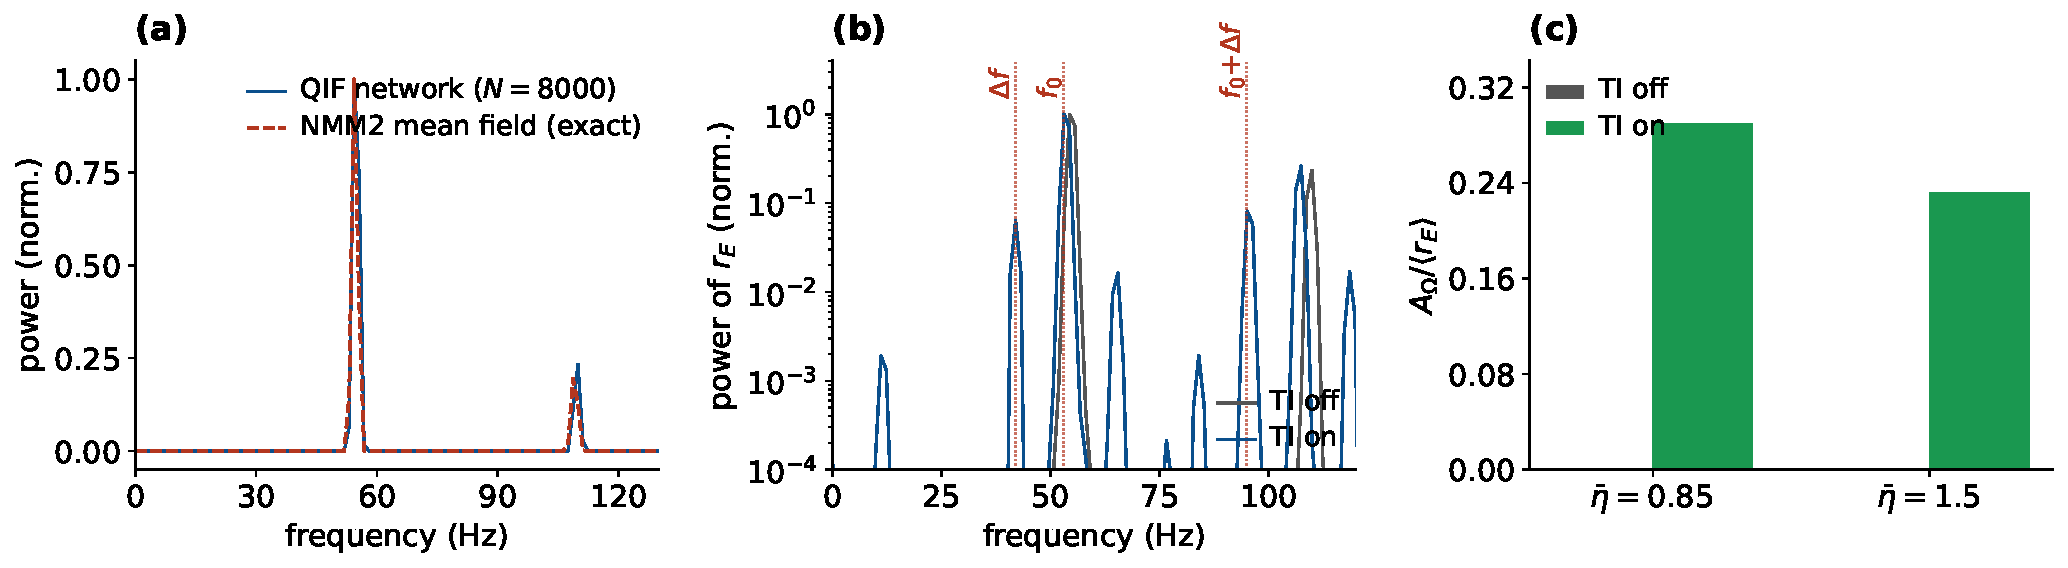
\includegraphics[width=\textwidth]{fig_qif_timing_twotone.pdf}
\caption{\DIFaddFL{\textbf{Beat-locked modulation and mean-rate change in the QIF network.} \emph{(a)} Field-free power
spectrum of $r_E(t)$, normalized: the spiking network ($N=8000$) matches the exact NMM2
mean field in gamma frequency ($\sim$55~Hz); a normalized spectrum does not test the mean
rate. \emph{(b)} Intermodulation above the
Hopf (TI off vs.\ on, log power): the nonlinearity mixes the imposed $\Delta f=42$~Hz beat
with the persisting gamma near $53$--$54$~Hz, raising the direct $\Delta f$ line and the sum sideband
near $95$~Hz, both absent with TI off. These sidebands establish nonlinear mixing;
they do not uniquely identify gamma-amplitude gating. \emph{(c)} The $\Delta f$ modulation depth
$A_\Omega/\langle r_E\rangle$, off vs.\ on: below $0.003$ rising to $0.29$
($\bar\eta=0.85$) and $0.23$ ($\bar\eta=1.5$), while the mean rate rises by about
$8$--$11\%$. The labels identify field-free states; both field-on responses contain
gamma activity beyond the beat component. Spectra use the same post-settling windows
as the rate measurements and are normalized to each spectrum's maximum. Modulation depth is
reported rather than the off$\to$on lock-in ratio, whose denominator is the field-free
floor.}}
\label{fig:qif_timing}
\end{figure}


\section{\DIFadd{Efficiency of a memoryless transfer against a direct in-band drive}}\label{app:bound}
\DIFadd{For the logistic family of memoryless transfers, compare balanced TI tones of
polarization amplitude $\varepsilon$ each with a direct in-band drive of amplitude
$2\varepsilon$, matching peak polarization. Their leading drive amplitudes are
$|\Sig''|\varepsilon^2/2$ and $2\Sig'\varepsilon$, so
$\mathcal R_{\rm det}\simeq|\Sig''|\varepsilon/(4\Sig')$.
The weak-input formula concerns the logistic family. The step-mixture argument
below extends the exact carrier-averaged bound to bounded nondecreasing
memoryless transfers, with the same operating point, matched peak polarization,
and open-loop readout. It does not cover the dynamic detector of \S\ref{sec:dynamic}.
}

\DIFadd{Writing $\zeta=\Sig/(2e_0)\in(0,1)$ gives
$\Sig'=2e_0\rho\zeta(1-\zeta)$ and
$\Sig''=2e_0\rho^2\zeta(1-\zeta)(1-2\zeta)$. Since
$|\mathrm{PEIX}|=1-4\zeta(1-\zeta)=(1-2\zeta)^2$, the leading ratio satisfies
}\begin{equation}
\DIFadd{\mathcal R_{\rm det}\simeq\frac{\rho\,\varepsilon}{4}\sqrt{|\mathrm{PEIX}|}
\;\le\;\frac{\rho\,\varepsilon}{4}.
\label{eq:etabound}
}\end{equation}
\DIFadd{It vanishes at the inflection, where the quadratic coefficient is zero, and
approaches its bound in the saturated tails. This maximizes a ratio rather than
an absolute response: both drives vanish in those tails. For the JR slope
$\rho=0.56$~mV$^{-1}$, the perturbative bound is $1.4\%$ at
$\varepsilon=0.1$~mV and $0.28\%$ at $\varepsilon=0.02$~mV.
}

\DIFadd{Optimizing over the sigmoid slope gives a different limit from the weak-input bound.
The logistic transfer depends on voltage only through $\rho(v-v_0)$, so writing
}\begin{equation}
\DIFadd{u=\rho\,\varepsilon,\qquad \xi=\rho\,(v^*-v_0),
\label{eq:reduced}
}\end{equation}
\DIFadd{we have $\Sig(v^*+\varepsilon\psi(t))=2e_0\,L(\xi+u\,\psi(t))$ for any normalized waveform $\psi$,
with $L(\xi)=(1+e^{-\xi})^{-1}$. Every Fourier amplitude, and hence their ratio, is a function
of $(u,\xi)$ alone; the factor $2e_0$ cancels. Maximizing over $v^*$ and $\rho$ at fixed
$\varepsilon$ is therefore the same as maximizing over $(u,\xi)$, and the family supremum is
independent of field strength. Evaluating the exact cycle response rather than its
quadratic truncation and optimizing $\xi$ at each $u$, the ratio rises monotonically over the
range explored and converges to the hard-threshold limit
}\begin{equation}
\DIFadd{\sup_{\rho,\,v^*}\mathcal R_{\rm det}\approx0.3479 ,
\label{eq:etasup}
}\end{equation}
\DIFadd{approached as $\rho\to\infty$ at a threshold offset $\delta$ (the distance from the
operating point to the inflection) with $\delta/2\varepsilon=0.523$. There is no
finite optimal transfer width: narrower is always better, and reaching $95\%$ of the ceiling
requires $u\gtrsim6$, that is $1/\rho\lesssim\varepsilon/6$.
}

\DIFadd{The limiting detector switches across its full range. At the optimum,
and at the illustrative fast-access polarization $\varepsilon\!\simeq\!0.1$~mV
of \S\ref{sec:discussion}, its open-loop beat drive
exceeds the physiological-slope sigmoid's by some three orders of magnitude for the same
$e_0$ and waveform, because the field excursion is about twice the threshold offset and the
transfer switches across its full range instead of responding linearly. The disparity grows
as the field weakens, the smooth sigmoid's response falling as $\varepsilon^2$ while a
threshold repositioned with the field keeps its excursion.
}

\DIFadd{The required transfer width is small: at $\varepsilon=0.1$~mV the ceiling is approached only for
$1/\rho\lesssim17\;\mu$V; at $\varepsilon=0.02$~mV the corresponding width is
about $3\;\mu$V. Both follow from $1/\rho\lesssim\varepsilon/6$, with the
threshold offset held to the same order as the applied polarization. A population
sigmoid averages the spread of thresholds and noise; the JR voltage scale is
$1/\rho\approx1.8$~mV \cite{jansen1995}. A
microvolt width lies far below that and reads as an idealized microscopic threshold or
rectifier rather than as a neural-mass sigmoid; real thresholds are themselves noisy and
state-dependent, so it is not a measured single-cell property either. The
regime in which the family approaches its ceiling is thus one in which the ``population
sigmoid'' has ceased to describe a population.
}

\DIFadd{The limit is a step detector, not an envelope follower. For a unit step at offset
$\delta$ the carrier-averaged transduction is $\pi^{-1}\arccos(\delta/\mathcal A)$ for $\mathcal A>\delta$
and zero below; with $\beta=\delta/2\varepsilon$ its tACS fundamental is
$(2/\pi)\sqrt{1-\beta^2}$ and its TI coefficient reduces by parts to
$\mathcal R_{\rm det}=2\beta\,[\mathsf K(k_{\rm ell}^2)-\mathsf E(k_{\rm ell}^2)]/(\pi\sqrt{1-\beta^2})$
with elliptic parameter $k_{\rm ell}^2=1-\beta^2$ and $\mathsf K,\mathsf E$
the complete elliptic integrals, giving $0.3479$ at $\beta=0.523$ by direct quadrature and
by the elliptic form alike (\texttt{threshold\_bound\_check.py}). At that optimum the
step's second-to-first harmonic magnitude ratio is $0.151$, not the $1/5$ of a linear
envelope follower. A bounded nondecreasing transfer is, up to a constant, a positive
mixture of shifted steps. Both signed Fourier coefficients are linear in the
transfer, and each step's direct-drive coefficient is nonnegative. The triangle
inequality therefore bounds the mixture's amplitude ratio by the largest step
ratio, whenever the denominator is nonzero. This extends the result beyond the
logistic family; the maximum itself is a numerical evaluation, not a certified bound.
}

\subsection{\DIFadd{Experimental amplitude and phase-locking comparisons}}\label{supp:vieira}
\DIFadd{The protocols in Vieira et al.\ \cite{vieira2024} do not match local polarization at the detector.
The two-pair TI comparison gave a phase-locking effect ratio of $0.34$ against
tACS (95\% confidence interval $0.04$--$0.65$, 65 of 154 neurons), without
correcting for TI currents up to $\pm2.5$~mA per pair versus $\pm1$~mA for tACS.
A separate single-pair AM-tACS control compensated for frequency-dependent
shunting to match extracellular modulation depth. Of twenty cells, ten responded
to either modality and seven to both; in the latter group, median phase-locking
value (PLV) was $0.10$ for AM-tACS and $0.20$ for tACS, against $0.043$ at baseline.
The reported TI modulation depths were about $0.5$--$0.62$~V/m.
}


\section{\DIFadd{Extension: the laminar column at low carriers}}\label{app:lanmm}
\DIFadd{The two-band laminar column (LaNMM) adds a resonant intermediary
between the field and the slow generator. These sweeps use $25$--$80$~Hz carriers
and polarizations up to $3$~mV on $P_2$, exceeding the sigmoid scale
$1/\rho\approx1.8$~mV. They describe nonlinear frequency selection below TI's
kHz range. The weak-field square law is tested separately in JR at
$0.05$--$0.2$~mV, one to two orders of magnitude below that scale
(Fig.~\ref{fig:opp}b).
}

\subsection{\DIFadd{Model and measurements}}\label{sec:lanmm-methods}
\DIFadd{The laminar extension (LaNMM)
\cite{ruffini2025cfc,sanchezTodo2023} adds coupled alpha and gamma circuits: deep
pyramidal $P_1$, spiny-stellate (SS), and somatostatin (SST) populations, and a
superficial pyramidal $P_2$/PV circuit.
We simulate this laminar neural mass model (LaNMM). We integrate the full 28-variable column
\cite{ruffini2025cfc,sanchezTodo2023}, with the field entering as in the single
JR column, as a membrane polarization added inside the sigmoid argument of the target
population. Its output rate $\varphi_X$ (s$^{-1}$) is
}\begin{equation}
\DIFadd{\varphi_X(t)=\Sig\!\big(v_X(t)+s(t)\big),\qquad X\in\{P_1,P_2\},
\label{eq:lanmm_drive}
}\end{equation}
\DIFadd{with $s(t)$ the AM or two-tone field of \S\ref{sec:coupling} (amplitude $\varepsilon$ in
mV, beat $\Omega=2\pi\Delta f$, carrier $\omega_c=2\pi f_c$) and all three external drives
held flat at their baselines (Fig.~\ref{fig:lanmm_setup}). A perturbation of an external
input \emph{rate} would require clipping at zero
once its excursion exceeds the baseline, and a hard clip is a half-wave rectifier---a
diode detector placed upstream of the sigmoid, which would inject a line at $\Delta f$
into the drive before the population nonlinearity received it. A signed membrane
polarization carries no such constraint and none is applied. Because the LaNMM and JR
sigmoids share the voltage scale $1/\rho\approx1.8$~mV, $\varepsilon$ is directly
comparable between the two models.
}

\DIFadd{Integration is a vectorized fixed-step RK4
($\Delta t=10^{-4}$~s) advancing the whole parameter grid simultaneously, as in the JR
sweeps. The maps report the
alpha-band ($8$--$12$~Hz) power of the $P_1$ and $P_2$ membrane potentials as the mean
squared magnitude of the Hann-windowed fast Fourier transform (FFT) over the band, in arbitrary units, over a
post-transient window. This measure includes autonomous and driven activity and
does not isolate a phase-coherent response to stimulation.
}

\DIFadd{Two sweeps probe the column: an amplitude--beat sweep over
$(\varepsilon,\Delta f)$ at fixed carrier, and a carrier--beat sweep
over $(f_c,\Delta f)$ at fixed $\varepsilon$, built on the LaNMM module of
\cite{ruffini2025cfc}. The maps
(Figs.~\ref{fig:lanmm_p2},~\ref{fig:lanmm_p1}) show the \emph{signed} stimulation-induced
change, alpha power minus the unstimulated ($\varepsilon=0$) baseline, on a zero-centered
scale; over most of the $P_1$-driven grids the change is negative. For the
alpha resonance we instead drive the deep $P_1$ loop directly and sweep its input against
$\Delta f$, reading the lock-in (}\ifsupp \DIFadd{main-text}\fi\DIFadd{\ Eq.~\eqref{eq:lockin}) of $v_{P_1}$ at $\Delta f$.
}

\DIFadd{The additional carrier comparison below uses the lock-in
of $v_{P_1}$, averaged at each carrier over 17 beats: $7$--$9$ and
$12.25$--$14$~Hz in $0.25$~Hz steps. These lie more than $1.5$~Hz from the
field-free alpha peak near $10.6$~Hz. We denote this arithmetic mean by $S(f_c)$.
The carrier grid is $25$--$80$~Hz in $1$~Hz steps, with equal tone amplitudes
$\varepsilon=1.5$~mV for $P_2$ drive and $0.5$~mV for $P_1$ drive. After $2$~s
of settling, we compare $3$ and $10$~s measurement windows. Field-free controls
give mean background amplitudes of $0.0048$ and $0.0012$~mV over the same beats.
This background includes a persistent component near $8$~Hz, so it is not solely
finite-window leakage. The statistic compares carrier profiles within each drive
condition; the unequal amplitudes do not support a direct sensitivity comparison
between targets.
}

\subsection{\DIFadd{Frequency selection and carrier dependence}}\label{sec:lanmm-results}
\DIFadd{Driving either population with the two-tone field of Eq.~\eqref{eq:lanmm_drive}
and reading alpha-band power in the deep ($P_1$, alpha) and superficial ($P_2$,
gamma) pyramidal potentials recovers the beat resonance
(\S\ref{sec:lanmm-methods}, Fig.~\ref{fig:lanmm_setup}). Direct $P_1$ drive reproduces the JR
alpha-band resonance on both stable-focus and limit-cycle sides; that sweep
and its code are in the repository. The additional result is carrier selectivity
through the coupled gamma circuit.
}

\DIFadd{Sweeping the field amplitude $\varepsilon$ and beat frequency $\Delta f$ at a fixed
carrier produces a region of enhanced alpha-band power: the response in $P_1$ is largest
when $\Delta f$ matches the deep alpha ($\sim$10~Hz) and grows with $\varepsilon$
(Figs.~\ref{fig:lanmm_p2}a,b and~\ref{fig:lanmm_p1}a,b). The dominant-frequency
contours identify where the output is close to the beat, without establishing
phase locking of the autonomous rhythm. Away from the enhancement region the drive
\emph{reduces} alpha-band power: with the field on $P_1$, $95\%$ of the amplitude--beat
grid and $97\%$ of the carrier--beat grid lie below the field-free baseline
(Fig.~\ref{fig:lanmm_p1}), the drive pulling the autonomous alpha out of the $8$--$12$~Hz
band or suppressing it; with the field on $P_2$ the fractions are $44\%$ and $31\%$
(Fig.~\ref{fig:lanmm_p2}).
}

\DIFadd{The carrier dependence illustrates the two coupling limits of
\S\ref{sec:coupling}--\S\ref{sec:khz} within this model's $25$--$80$~Hz carrier
range. When the field is delivered to the superficial loop ($P_2$), alpha-band
power enhancement in $P_1$ is largest in the gamma carrier band with
$\Delta f$ near the $P_1$ alpha (Fig.~\ref{fig:lanmm_p2}c,d). At
$\Delta f=10$~Hz, the carrier maximum is $44$~Hz. This selectivity is consistent with a double
resonance: the fast loop acts as a tuned
radio-frequency (RF) front end whose dynamics affect the carrier dependence of
the deep response. With direct $P_1$ drive, a ridge near the column's own alpha
persists across the carrier range (Fig.~\ref{fig:lanmm_p1}c). That ridge contains
autonomous activity and is not a measurement of the demodulated component alone.
}

\DIFadd{The lock-in also contains the autonomous rhythm when the beat is close to alpha;
its maximum over beats cannot isolate the driven response. We therefore compare
the off-alpha statistic $S(f_c)$ defined in \S\ref{sec:lanmm-methods}
(Table~\ref{tab:lanmm-carrier}).
With $P_2$ drive it peaks near $39$~Hz and falls to about $16$--$17\%$ of that
peak at a $25$~Hz carrier. With $P_1$ drive it peaks at $25$~Hz and spans about
$42$--$68\%$ of that peak over $30$--$80$~Hz. These are properties of the
specified amplitudes and beat average, not universal carrier-rejection factors.
Single-beat profiles have deeper minima, including a dip near a $45$~Hz carrier
under direct $P_1$ drive: the gamma circuit can affect the response in either
stimulation condition.
}

\begin{table}[t!]
\centering\small
\caption{\DIFaddFL{\textbf{LaNMM carrier profiles measured away from alpha.}
$S(f_c)$ is the mean lock-in amplitude of $v_{P_1}$ over the 17 beats specified
in \S\ref{sec:lanmm-methods}. Percentages are normalized to each row's own carrier maximum;
the range and median use carriers from $30$ to $80$~Hz.}}
\label{tab:lanmm-carrier}
\begin{tabular}{@{}llrrrr@{}}
\toprule
\DIFaddFL{Drive }& \DIFaddFL{Window }& \DIFaddFL{Peak $S$ (mV) }& \DIFaddFL{Peak $f_c$ (Hz) }& \DIFaddFL{Range (\%) }& \DIFaddFL{Median (\%)}\\
\midrule
\DIFaddFL{$P_2$, $1.5$ mV }& \DIFaddFL{$3$ s  }& \DIFaddFL{$0.450$ }& \DIFaddFL{$39$ }& \DIFaddFL{$23$--$100$ }& \DIFaddFL{$42$}\\
\DIFaddFL{$P_2$, $1.5$ mV }& \DIFaddFL{$10$ s }& \DIFaddFL{$0.450$ }& \DIFaddFL{$39$ }& \DIFaddFL{$23$--$100$ }& \DIFaddFL{$42$}\\
\DIFaddFL{$P_1$, $0.5$ mV }& \DIFaddFL{$3$ s  }& \DIFaddFL{$0.092$ }& \DIFaddFL{$25$ }& \DIFaddFL{$42$--$68$  }& \DIFaddFL{$53$}\\
\DIFaddFL{$P_1$, $0.5$ mV }& \DIFaddFL{$10$ s }& \DIFaddFL{$0.091$ }& \DIFaddFL{$25$ }& \DIFaddFL{$42$--$67$  }& \DIFaddFL{$52$}\\
\bottomrule
\end{tabular}
\end{table}

\DIFadd{The carrier peaks and aggregate ranges persist with the longer window, although
individual normalized values change by up to $3.1$ percentage points for $P_2$
drive and $9.6$ for $P_1$ drive. The smallest $S$ exceeds its mean field-free
background by factors of about $16$ and $8$, respectively, with the $3$~s window,
and $62$ and $32$ with $10$~s. Some individual beat--carrier points remain near or below
background; the comparison concerns the mean over beats, not each grid point.
TI's kHz carriers lie outside this model's range. Within it, the carrier can
excite a network mode and affect the detected response, qualifying the inert-carrier
limit of \S\ref{sec:carrier} and linking it to frequency-tagging and
intermodulation paradigms \cite{gordon2019}.
}

\setcounter{figure}{0}
\begin{figure}[t!]
\centering
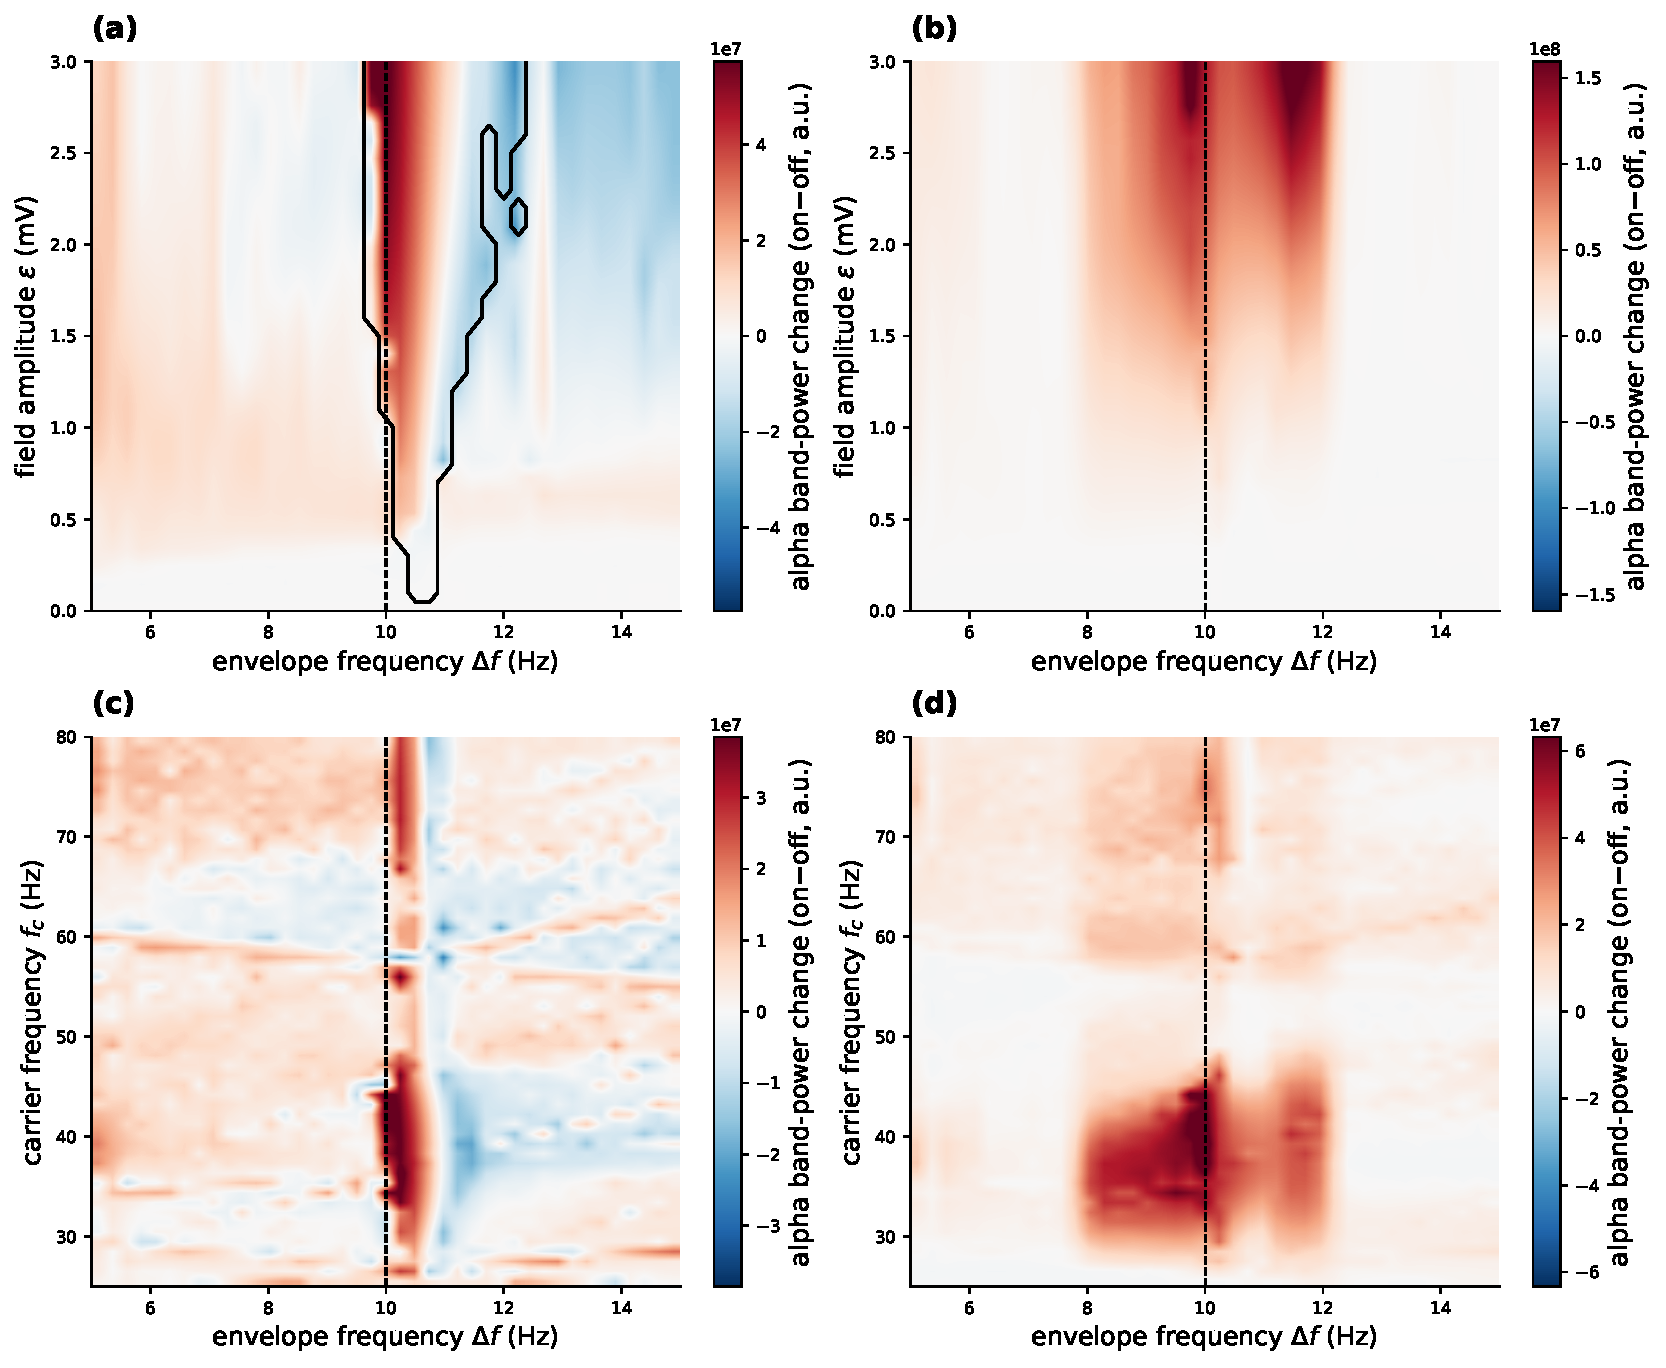
\includegraphics[width=0.86\textwidth]{fig_lanmm_field_p2_twotone.pdf}
\caption{\DIFaddFL{\textbf{LaNMM frequency selection: two-tone TI field on the superficial $P_2$ (gamma)
loop.} The field enters the $P_2$ sigmoid argument as a membrane polarization $\varepsilon$
(mV) with all external drives flat. Color shows the signed change of alpha-band
($8$--$12$~Hz) power from the unstimulated $\varepsilon=0$ baseline, on a zero-centered
scale (arbitrary units). \emph{(a,b)} $P_1$ and $P_2$ enhancement vs.\
$\varepsilon$ and $\Delta f$ (carrier $40$~Hz), peaking at the $P_1$ alpha ($10.0$~Hz,
dashed). The black contour in \emph{(a)} is the frequency-dominance set
$|f_{\rm out}-\Delta f|<0.3$~Hz, drawn because band power
alone cannot separate a driven from an autonomous rhythm; it is a dominance screen, not a
phase-capture test. The $\varepsilon=0$ row is excluded, since with no drive the
autonomous $10.67$~Hz alpha already lies within the tolerance of two grid points (a
resolution floor of $0.5$~Hz); the set widens to $2.75$~Hz at $3$~mV. \emph{(c,d)} Enhancement vs.\ carrier and $\Delta f$ at
$\varepsilon=1.5$~mV: $P_1$ alpha-band enhancement is largest in the
gamma carrier band with $\Delta f$ near the $P_1$ alpha. At $\Delta f=10$~Hz,
the carrier maximum is $44$~Hz. The field-free
$P_2$ gamma peak is near $39.7$~Hz; the finite-drive maximum need not coincide with it.}}
\label{fig:lanmm_p2}
\end{figure}



\DIFadd{Within the $25$--$80$~Hz carrier range and at the finite polarizations used here,
the LaNMM shows alpha-band power changes concentrated near the intrinsic alpha,
amplitude-dependent widening of the frequency-dominance region, and enhanced
responses when superficial drive passes through the gamma circuit. The power
maps include autonomous and driven activity; they do not isolate TI efficacy.
The gamma-carrier preference, around $40$~Hz rather than kHz, remains a separate
prediction to test. Esmaeilpour et al.\ \cite{esmaeilpour2021} swept
$0.1$--$2$~kHz carriers at a fixed $5$~Hz beat against carbachol-induced gamma,
finding decreasing sensitivity with carrier frequency. Those carriers did not
sample the gamma band. Violante et al.\ \cite{violante2023} also used a fixed
$5$~Hz beat. Neither study tests this low-carrier resonance prediction.
}

\setcounter{figure}{1}
\begin{figure}[t!]
\centering
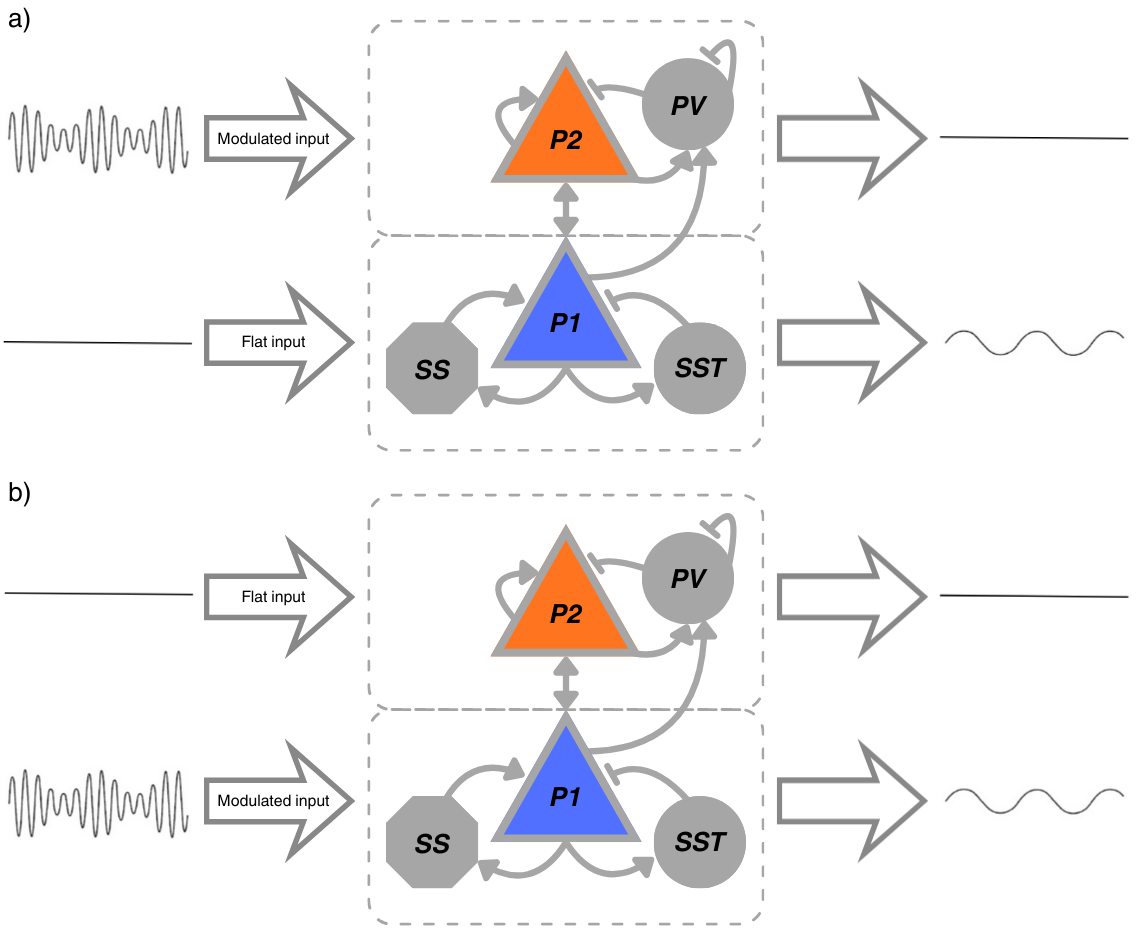
\includegraphics[width=0.85\textwidth]{fig_lanmm_setup.png}
\caption{\DIFaddFL{\textbf{Stimulation setup in a LaNMM column.} The column couples a
superficial PING subcircuit (pyramidal $P_2$ + PV; gamma) and a deep JR
subcircuit (pyramidal $P_1$ + SS + SST; alpha). \emph{(a)} the TI field drives
$P_2$ while $P_1$ receives a flat drive; \emph{(b)} the TI field drives $P_1$
while $P_2$ is flat. Through the sigmoid nonlinearities and $P_1$--$P_2$ coupling,
the generated beat-frequency component is transferred to the deep loop: $P_2$ carries the
modulated fast carrier, while $P_1$ exposes the recovered low-frequency component (right
traces).}}
\label{fig:lanmm_setup}
\end{figure}

\setcounter{figure}{6}
\begin{figure}[t!]
\centering
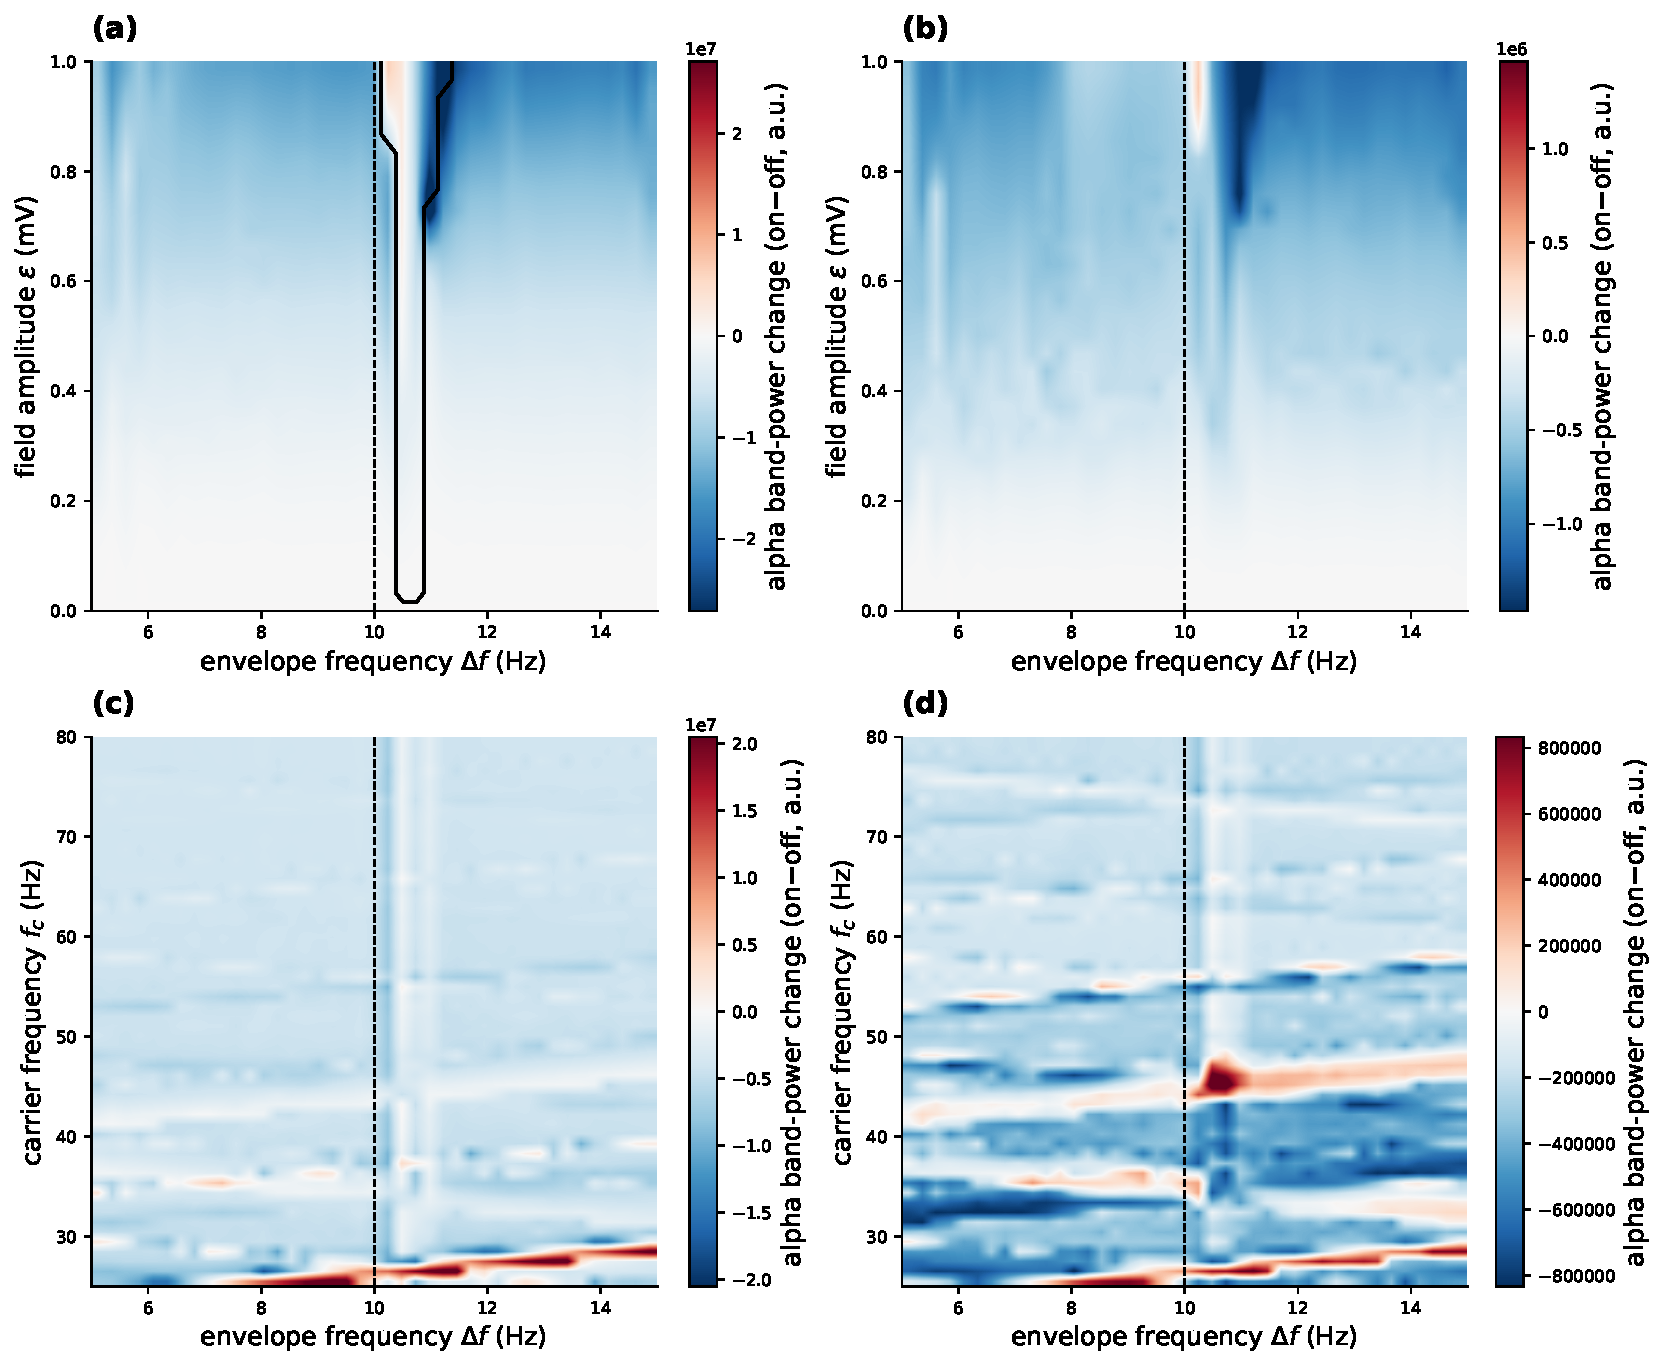
\includegraphics[width=0.86\textwidth]{fig_lanmm_field_p1_twotone.pdf}
\caption{\DIFaddFL{\textbf{LaNMM frequency selection: two-tone TI field delivered directly to the deep
$P_1$ (alpha) loop.} As Fig.~\ref{fig:lanmm_p2} but with the field on $P_1$. The deep loop
shows frequency dominance at smaller fields, so the amplitude range is
$\varepsilon\le1$~mV here against $3$~mV there. These finite-amplitude maps extend
beyond the perturbative regime of the theory. Color: signed change of alpha-band power from the $\varepsilon=0$ baseline,
zero-centered; most of the grid is suppression. \emph{(a,b)} $P_1$ and $P_2$ enhancement vs.\ $\varepsilon$ and $\Delta f$; the
black contour in \emph{(a)} outlines the frequency-dominance set
$|f_{\rm out}-\Delta f|<0.3$~Hz (\S\ref{sec:vocab}), computed from the dominant
output frequency because band power alone cannot separate a driven from an autonomous
rhythm; the $\varepsilon=0$ row is excluded (resolution floor $0.5$~Hz). The set widens to
$1.25$~Hz at $\varepsilon=1$~mV.
\emph{(c,d)} Enhancement vs.\ carrier frequency and $\Delta f$ at $\varepsilon=0.5$~mV.
The ridge near alpha persists across the carrier band and includes the autonomous
rhythm. A separate lock-in comparison away from alpha, including its window and
background controls, is given in Table~\ref{tab:lanmm-carrier}; these panels show
band-power changes.}}
\label{fig:lanmm_p1}
\end{figure}


\section{\DIFadd{Vocabulary and numerical settings}}\label{sec:vocab}
\DIFadd{\emph{Forced response.} Below the Hopf the column does not oscillate on its own;
we quantify its response by the lock-in amplitude at the beat $\Delta f$
(}\ifsupp \DIFadd{main-text}\fi\DIFadd{\ Eq.~\eqref{eq:lockin}). There is no autonomous rhythm to entrain in the stable-focus
J-curve, timing, and tACS sweeps.
}

\DIFadd{\emph{Frequency dominance and entrainment.} Above the Hopf the column free-runs
at $f_0$. A $1{:}1$ phase-capture test would follow the unwrapped phase difference
from the drive and require absence of secular drift. Our maps instead report
$|f_{\rm out}-\Delta f|<0.3$~Hz, where $f_{\rm out}$ is the largest non-DC FFT
peak. This is a frequency-dominance screen: a forced component can outgrow a
persisting autonomous one without capturing it. When the components coexist,
instantaneous-phase estimates also require their separation
\cite{lachaux1999}. The maps therefore identify a dominance region, not a
measured Arnold tongue.
}

\DIFadd{\emph{Beat-locked rate and gating.} Gating means that the amplitude of a
persisting rhythm is modulated by the beat without frequency capture
\cite{canolty2010,tort2010}. The QIF statistic used here is the lock-in of the
population rate $r_E$ at $\Delta f$, complemented by the rate folded on beat
phase over whole cycles. It measures beat-locked firing. A raw rate fold does
not extract the gamma amplitude, and sidebands can arise from amplitude or phase
modulation. The above-Hopf QIF panels therefore establish coexistence and mixing
of the beat and gamma rhythms; a gamma-amplitude estimate would be needed to
identify gating specifically.
}

\DIFadd{The protocol for Fig.~\ref{fig:entrain} places the column on the limit-cycle side
(input $p$ on the stable alpha-cycle branch below its upper Hopf), drives it
with $s(t)=\varepsilon\cos\Omega t$, and records the dominant frequency. Grid
widths and the clipping check are specified in the code. As the Hopf is approached,
the autonomous cycle shrinks and the frequency-dominance region broadens in these
simulations. Its width and the stable-focus susceptibility describe different
responses; their increase near onset does not make them the same quantity.
}

\ifjne
\subsection{\DIFadd{Lock-in leakage control}}\label{supp:lockin}
\DIFadd{Out-of-band components can leak into the estimate, particularly the DC level of the JR voltage readout ($\bar v\!\sim\!8$~mV, far
larger than the demodulated signal). The finite-window projection of a constant onto the quadrature references
need not vanish, so we subtract $\bar v$ explicitly; this makes the metric
accurate down to the $10^{-8}$ level needed for the JR kHz
analysis.
}

\subsection{\DIFadd{JR integration and measurement windows}}\label{supp:jr-runs}
\DIFadd{We integrate with a fixed-step fourth-order Runge--Kutta (RK4) scheme,
$\Delta t=2\times10^{-4}$~s (50 samples per carrier cycle at $100$~Hz; reduced to
$10^{-4}$~s for carrier sweeps up to $300$~Hz). The kHz-carrier runs of
Fig.~\ref{fig:khz_direct} use $\Delta t=2\times10^{-5}$~s for the carrier sweep to
$4$~kHz (25 samples per carrier cycle at $2$~kHz, 12.5 at $4$~kHz) and
$1.5\times10^{-5}$~s for the $2$~kHz output spectrum. Halving each step changes the
reported lock-in amplitudes by less than $1\%$. The $10$~kHz figures quoted in
\S\ref{sec:khz} are analytic evaluations of Eq.~\eqref{eq:khz}, not simulations.
}

\DIFadd{The resonance sweep uses $10$~s of settling and a $20$~s
measurement window. Long windows reduce transients from weakly damped modes and
average beating when autonomous activity persists. Other runs use the windows
specified in their scripts.
The two-tone $2$~kHz example (Fig.~\ref{fig:khz_twotone}) uses $p=400$~s$^{-1}$,
$C=135$, and $0.5$~mV per tone with $\tau=0.2$~ms. From a zero initial state,
it settles for $4$~s and records $4$~s at $\Delta t=1.5\times10^{-5}$~s,
sampling before each RK4 step. Its amplitude spectra use plain-mean subtraction
and a Hann window. Parameter sweeps advance all $N_{\rm grid}$ combinations simultaneously
in a vectorized $(N_{\rm grid},6)$ state array.
}

\fi

\ifsupp
\clearpage
\bibliographystyle{unsrt}
\bibliography{references}
\fi
\fi
 \DIFaddend\end{document}
